\documentclass[twoside,colorback,accentcolor=tud4c,11pt]{tudreport}
\usepackage[english]{babel}

\usepackage[stable]{footmisc}
\usepackage[ngerman,pdfview=FitH,pdfstartview=FitV]{hyperref}

\usepackage{booktabs}
\usepackage{multirow}
\usepackage{longtable}



\usepackage{mathtools}
\usepackage[stable]{footmisc}
\usepackage{float}
\usepackage{amsthm}
\usepackage{amsmath}
\usepackage{graphicx}
\usepackage{subcaption}
\usepackage{listings}


\newlength{\longtablewidth}
\setlength{\longtablewidth}{0.675\linewidth}

\title{Optimal Harvesting Modelling}
\subtitle{Final Report}
%\subsubtitle{email: \textaccent{tud-design@pro-kevin.de}}
%\uppertitleback{(\textaccent{\textbackslash uppertitleback})}
%\lowertitleback{(\textaccent{\textbackslash lowertitleback})\hfill\today}
\institution{Centre de Recerca Matem\`atica\\ Universitat Auton\`onoma de Barcelona \\ Group number 4.}



\newtheorem{theorem}{Theorem}
\newtheorem{definition}{Definition}
\newtheorem{corollary}{Corollary}
\newtheorem{lemma}{Lemma}



\newcommand{\asterisk}[1]{{#1}^{\ast}}
\newcommand{\nabladot}{\nabla\cdot}
\newcommand{\diff}[1]{\mathrm{d} #1}
\newcommand{\dev}[2]{\frac{\mathrm{d} #1}{{\mathrm{d} #2}}}
\newcommand{\ddev}[2]{\frac{\mathrm{d}^2 #1}{{\mathrm{d}#2}^2}}
\newcommand{\grad}[1]{\nabla\left(#1\right)}
\newcommand{\spdev}[2]{\frac{\partial ^{2} #1}{{\partial #2}^{2}}}
\newcommand{\ppdev}[2]{\frac{\partial ^{2} #1}{{\partial #2}^{2}}}
\newcommand{\pdev}[2]{\frac{\partial #1}{{\partial #2}}}
\newcommand{\pdxo}{\partial_{\asterisk{x}}}
\newcommand{\pdyo}{\partial_{\asterisk{y}}}
\newcommand{\pddxo}{\partial_{\asterisk{x}}^2}
\newcommand{\pddyo}{\partial_{\asterisk{y}}^2}

\newcommand\norm[1]{\left\lVert #1 \right\rVert}
\newcommand\abs[1]{\left|#1\right|}
\newcommand\argmin[2]{
{\displaystyle {\underset {#1}{\operatorname {arg\,min} }}\left[#2\right]}}
\newcommand\Min[2]{
	{\displaystyle {\underset {#1}{\min\, }}#2}}
\newcommand\epi{\mathrm{epi\,}}
\newcommand\dom{\mathrm{dom\,}}
\newcommand\cone{\mathrm{cone\,}}
\newcommand{\dive}{\mathrm{div\,}}
\newcommand{\prox}[2]{{\displaystyle {\underset {#1}{\operatorname {prox} }}#2}}
\newcommand{\interior}[1]{\widering{#1}}

\begin{document}
\maketitle
\begin{abstract}
	
\end{abstract}  

\tableofcontents
%\chapter{Preliminary Concept} \label{chap:Preliminary}
%\section{Constrained minimization in Banach spaces and Lagrange multipliers}

\begin{definition}{Lower semi-continuous} A functional $F$ is lower-semicontinuous if
	\begin{equation}
		F\left(\lim_{n\rightarrow\infty}x_n\right) \leq \liminf_{n\rightarrow \infty} F(x_n)
	\end{equation}
	
\end{definition}
	
\begin{definition}{Derivative.} The functional $F$ on a Banach space i
	
\end{definition}



Let $X$, $Y$, $U$ be Hilbert spaces and Z be a Hilbert lattice. 
Consider the constrained minimization problem:
\begin{equation*}
	\min_{x\in C} J(x)
\end{equation*}
subject to 
\begin{gather*}
	E(x)=0 \\ \text{and} \\ G(x)\leq 0
\end{gather*}
Where $C$ is a closed and convex set in $X$, $J: X \rightarrow \mathbb{R}$, $E: X\rightarrow Y$, and $G: X \rightarrow Z$ are continuously differentiable
\section{Control Problem}

\chapter{Problem Description and Framework}\label{chap:Problem Framework}
\graphicspath{{ProblemFramework/}}
\begin{equation}
\dev{x}{t}=rx\left(1-\frac{x}{M}\right)-u \label{eq: ConstantHarvest}
\end{equation}
We introduce the following variable in order to simply calculations,
\begin{equation}
\beta=\frac{uM}{r}
\end{equation}
Solving the differential equation,
\begin{align*}
	\frac{\diff{x}}{rx\left(1-\frac{x}{M}\right)-u}&=\diff{t} \\
	\int_{x_0}^{x}\frac{\diff{\chi}}{r\chi\left(1-\frac{\chi}{M}\right)-u}&=\int_{0}^{t}\diff{\tau} \\
	\frac{M}{r}\int_{x_0}^{x}\frac{\diff{\chi}}{\chi\left(M-\chi\right)-\frac{Mu}{r}}&=t \\
	-\frac{M}{r}\int_{x_0}^{x}\frac{\diff{\chi}}{\chi^2-M\chi+\beta}&=t \nonumber
	\end{align*}
Finally, we model the above integral as one 
\begin{align}
	-\frac{M}{r}\int_{x_0}^{x}\frac{\diff{\chi}}{\left(\chi-\frac{M}{2}\right)^2-\frac{M^2}{4}+\beta}&=t
\end{align}
Consider $\alpha$ as follows,
\begin{equation}
	\alpha = \beta - \frac{M^2}{4} = rM\left(u-\frac{rM}{4}\right)
\end{equation}
We see that the sign of $\alpha$ determines the nature of the solutions. Then, if $u>rM/4$ implies $\alpha>0$,
\begin{align*}
\int_{x_0}^{x}\frac{\diff{\chi}}{\left(\chi-\frac{M}{2}\right)^2+\alpha}&=-\frac{r}{M}t \\
\frac{1}{\sqrt{\beta-\frac{M^2}{4}}}\left(\arctan\left(\frac{x-M/2}{\sqrt{\beta-M^2/4}}\right)-\arctan\left(\frac{x_0-M/2}{\sqrt{\beta-M^2/4}}\right)\right)&=-\frac{r}{M}t \\
\end{align*}
Therefore, for $\alpha > 0$ the population behaves as follows, 
\begin{align}
	x(t)=\frac{M}{2}+\sqrt{\beta-\frac{M^2}{4}} \tan \left(\arctan\left(\frac{x_0-M/2}{\sqrt{\beta-M^2/4}}\right)-\frac{r\sqrt{\beta-M^2/4}}{M}t\right) \label{eq: ConstantHarvest OverExploit}
\end{align}

Equation \ref{eq: ConstantHarvest OverExploit} show us that for some $t^*$, $x(t^*)=0$,independently of the initial condition $x_0$, since the argument inside the $\tan$ is monotone decreasing in $t$. 

If $u<rM/4$ implies $-\alpha>0$,
\begin{align*}
	\int_{x_0}^{x}\frac{\diff{\chi}}{\left(\chi-\frac{M}{2}\right)^2-(-\alpha)} &=-\frac{r}{M}t
\end{align*}
Considering the zeros of the denominator, $\lambda$ and $\overleftarrow{\lambda}$, 
\begin{equation}
	\begin{array}{cc}
	\lambda&=\frac{M}{2}+\sqrt{\frac{M^2}{4}-\beta} \\
	\overline{\lambda}&=\frac{M}{2}-\sqrt{\frac{M^2}{4}-\beta} \\
	\end{array}
\end{equation}
We can rewrite our expression as follows, 
\begin{align*}
\int_{x_0}^{x} \left(\frac{1}{\chi - \lambda}-\frac{1}{\chi - \overline{\lambda}}\right)\diff{\chi} &=-\frac{2r\sqrt{M^2/4-\beta}}{M}t \\
	\ln\abs{\frac{x - \lambda}{x - \overline{\lambda}}}&=\ln\abs{\frac{x_0- \lambda}{x_0 - \overline{\lambda}}}-\frac{2r\sqrt{M^2/4-\beta}}{M}t
\end{align*}
For simplifying calculations, we write, $\gamma=\frac{2r\sqrt{M^2/4-\beta}}{M}$. And we obtain as result,
\begin{align}
\frac{x - \lambda}{x - \overline{\lambda}} &=\frac{x_0- \lambda}{x_0- \overline{\lambda}}\mathrm e^{-\gamma t} \\
x-\lambda &=\left(x-\overline{\lambda}\right)\left(\frac{x_0- \lambda}{x_0- \overline{\lambda}}\right)\mathrm e^{-\gamma t}
\end{align}

For the sake of simplicity, consider $\xi=\frac{x_0-\lambda}{x_0-\overline{\lambda}}\mathrm{e}^{-\gamma t}$. Therefore,
\begin{align*}
	x\left(1-\xi\right)&=\lambda-\overline{\lambda}\xi\\
	x&=\frac{\lambda-\overline{\lambda}\xi}{1-\xi} \\	
	x&=\frac{\frac{M}{2}+\sqrt{\frac{M^2}{4}-\beta}-\left(\frac{M}{2}-\sqrt{\frac{M^2}{4}-\beta}\right)\xi}{1-\xi}\\
	x&=\frac{\frac{M}{2}+\sqrt{\frac{M^2}{4}-\beta}-\left(\frac{M}{2}-\sqrt{\frac{M^2}{4}-\beta}\right)\xi}{1-\xi}\\
	x&=\frac{\frac{M}{2}\left(1-\xi\right)+\sqrt{\frac{M^2}{4}-\beta}\left(1+\xi\right)}{1-\xi}\\
	x&=\frac{M}{2}+\sqrt{\frac{M^2}{4}-\beta}\frac{1+\xi}{1-\xi}
\end{align*}
Hence, for $-\alpha>0$, we have the following result,
\begin{align}
	x(t)&=\frac{M}{2}+\left(\sqrt{\frac{M^2}{4}-\beta}\right)\frac{\left(x_0-M/2\right)\left(1+\mathrm e^{-\gamma t}\right)-\sqrt{M^2/4-\beta}\left(1-\mathrm{e}^{-\gamma t}\right)}{\left(x_0-M/2\right)\left(1-\mathrm e^{-\gamma t}\right)+\sqrt{M^2/4-\beta}\left(1+\mathrm{e}^{-\gamma t}\right)} \label{eq: Time Expression for Harvest}
\end{align}

If $u=\frac{rM}{4}$, we solve equation \ref{eq: ConstantHarvest} as follows,
\begin{align}
-\frac{M}{r}\int_{x_0}^{x}\frac{d\chi}{\left(\chi-\frac{M}{2}\right)^2}&=t\\
\int_{x_0}^{x}\frac{d\chi}{\left(\chi-\frac{M}{2}\right)^2}&=-\frac{rt}{M}\\
\frac{1}{x-\frac{M}{2}}&=\frac{1}{x_0-\frac{M}{2}}-\frac{rt}{M}\\
\frac{1}{x-\frac{M}{2}}&=\frac{M-\left(x_0-\frac{M}{2}\right)rt}{M\left(x_0-\frac{M}{2}\right)} \\
x&=\frac{M}{2}+\frac{M\left(x_0-\frac{M}{2}\right)}{M-\left(x_0-\frac{M}{2}\right)rt} 
\end{align}

The results above stated can be explained directly from the equation \ref{eq: ConstantHarvest}, as we see in the graph \ref{fig: CriticalPoints},  $F(x,t)$ is a paraboloid, with its maximum at $F(x^*=M/2,t)=rM^2/4$.

When $u=0$, we have the regular logistic equation with critical points $x_{c_1}=0$ and $x_{c_2}=M$. With $x_{c_2}$ being an stable fixed point and $x_{c_1}$ an unstable fixed point. In general, these are the solutions to the equation $F(x,t)-u=0$,
\begin{equation}
x_{c_{2,1}}=\frac{M}{2}\pm \sqrt{\frac{M^2}{4}-u\frac{M}{r}}
\end{equation}

We observe that the critical points $x_c$, such that $\dev{x_c}{t}=F(x_c, t)-u=0$ are getting closer to each other, as $u$ is increasing; when $u=\frac{rM}{4}$ we only have one critical unstable point. That behaves as an attractor when $x_0\geq\frac{M}{2}$. But when $x_0<\frac{M}{2}$ the population strictly decreases. For $u> \frac{rM}{4}$, the population $x(t)$ has no real critical points and the derivative $\dev{x}{t}$ is always negative, implying, that we will lead always the population to extinction, extracting constantly at a rate greater than $\frac{rM}{4}$.

\begin{figure}[H]
	\centering
	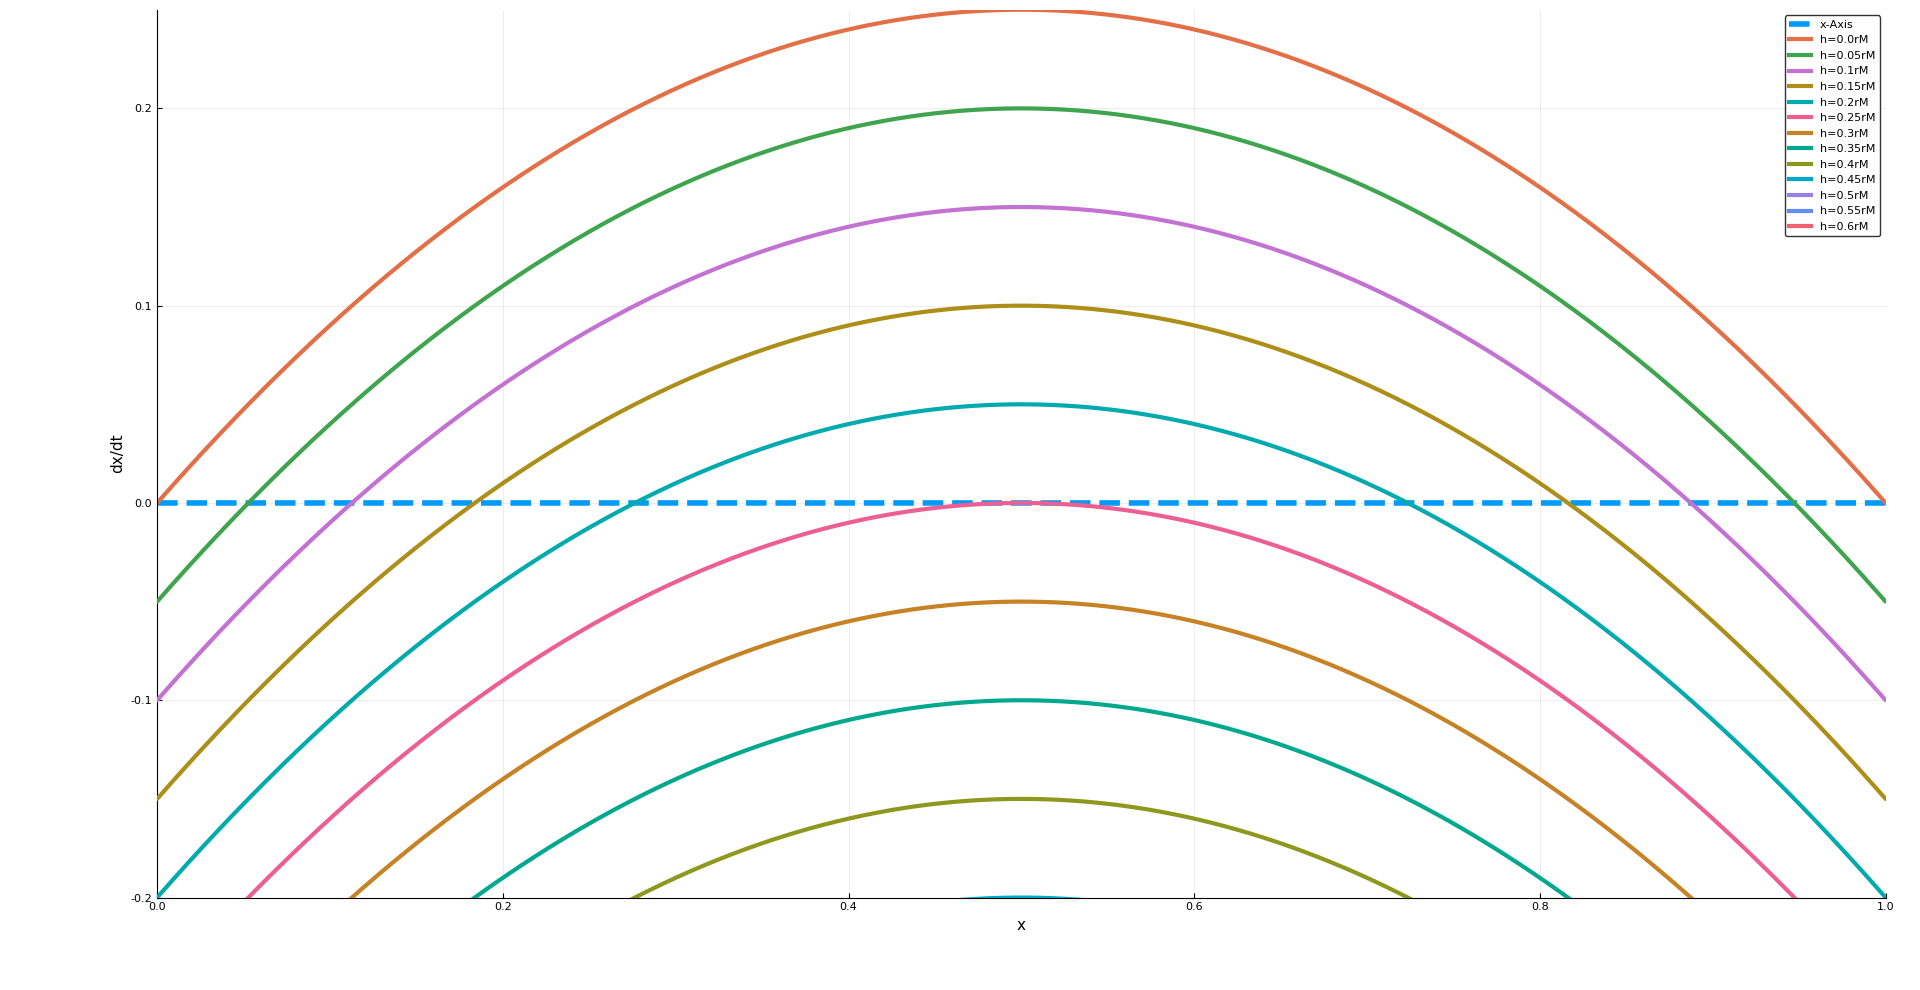
\includegraphics[width=0.8\textwidth]{CriticalPoints.png}
	\caption{Figure representing $\dev{x}{t}$ with different harvesting rates.}
	\label{fig: CriticalPoints}
\end{figure}
\begin{figure}
		\centering
		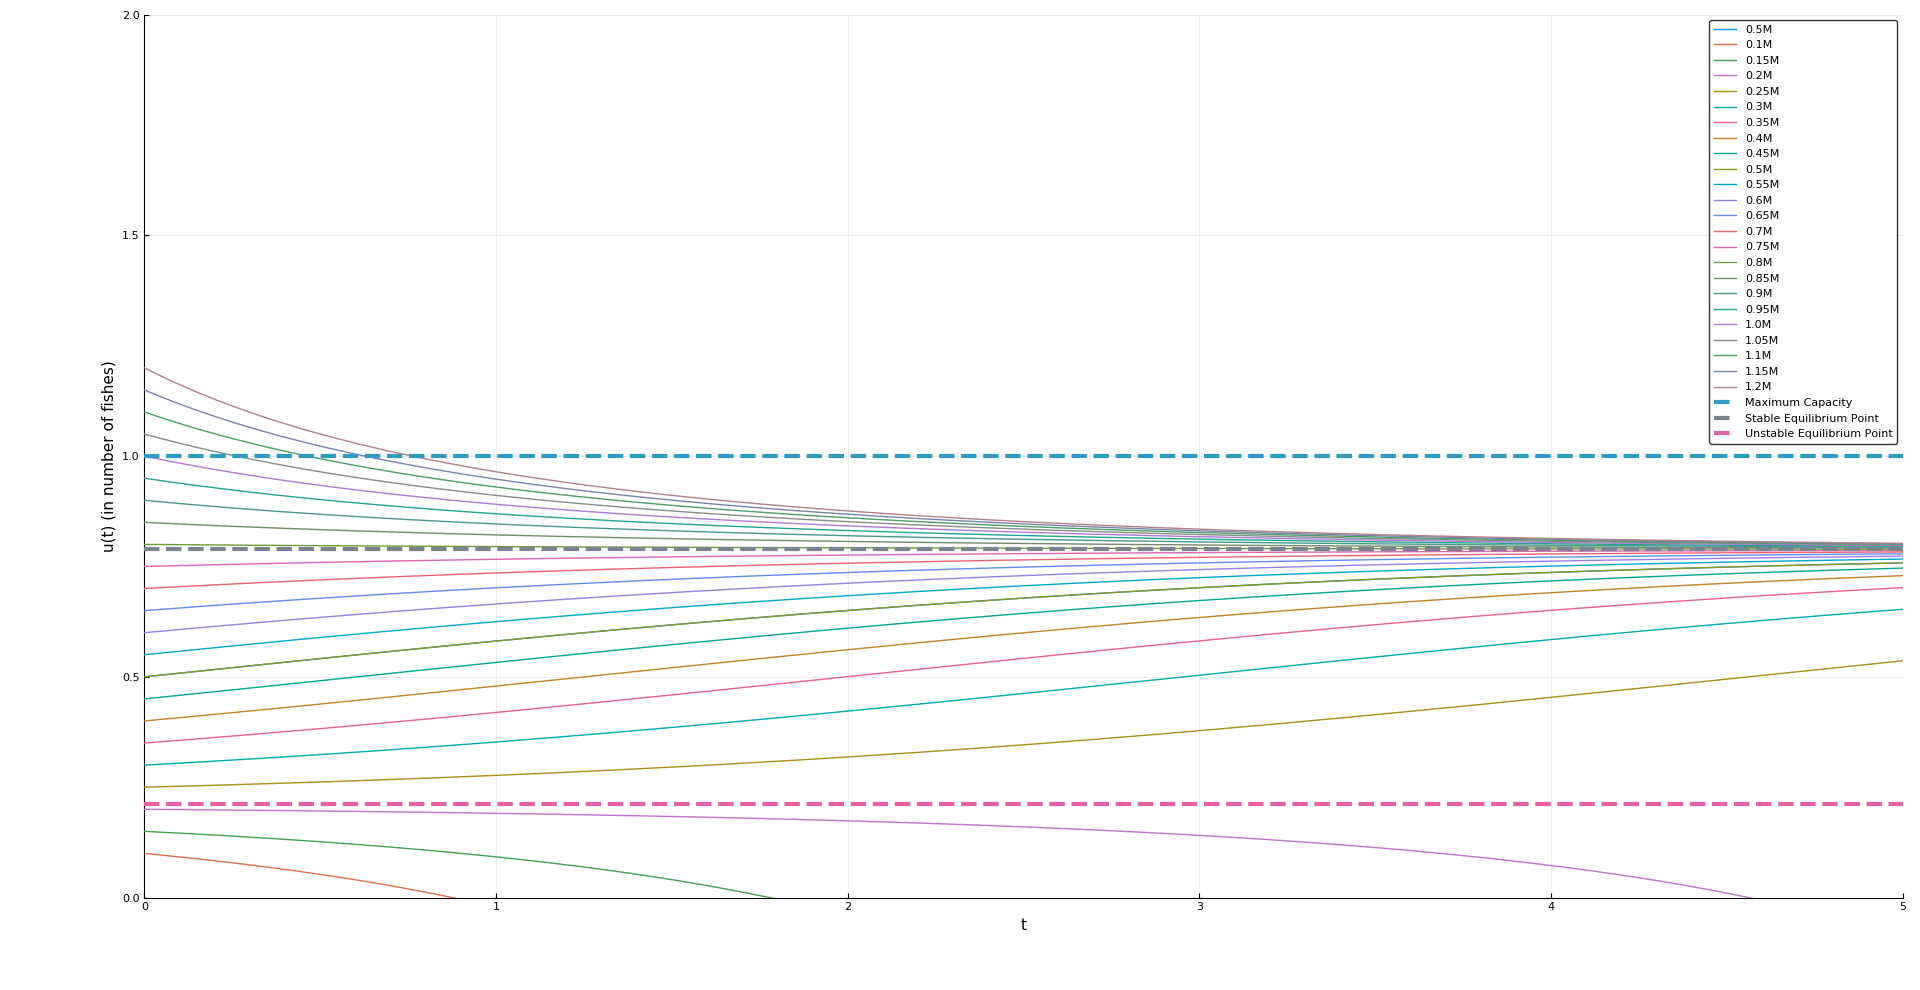
\includegraphics[width=0.8\textwidth]{SustainableConstant.png}
		\caption{Constant harvest rate $u<\frac{rM}{4}$.}
		\label{fig: SustainableConstantHarvest}
\end{figure}
\begin{figure}
	\centering
	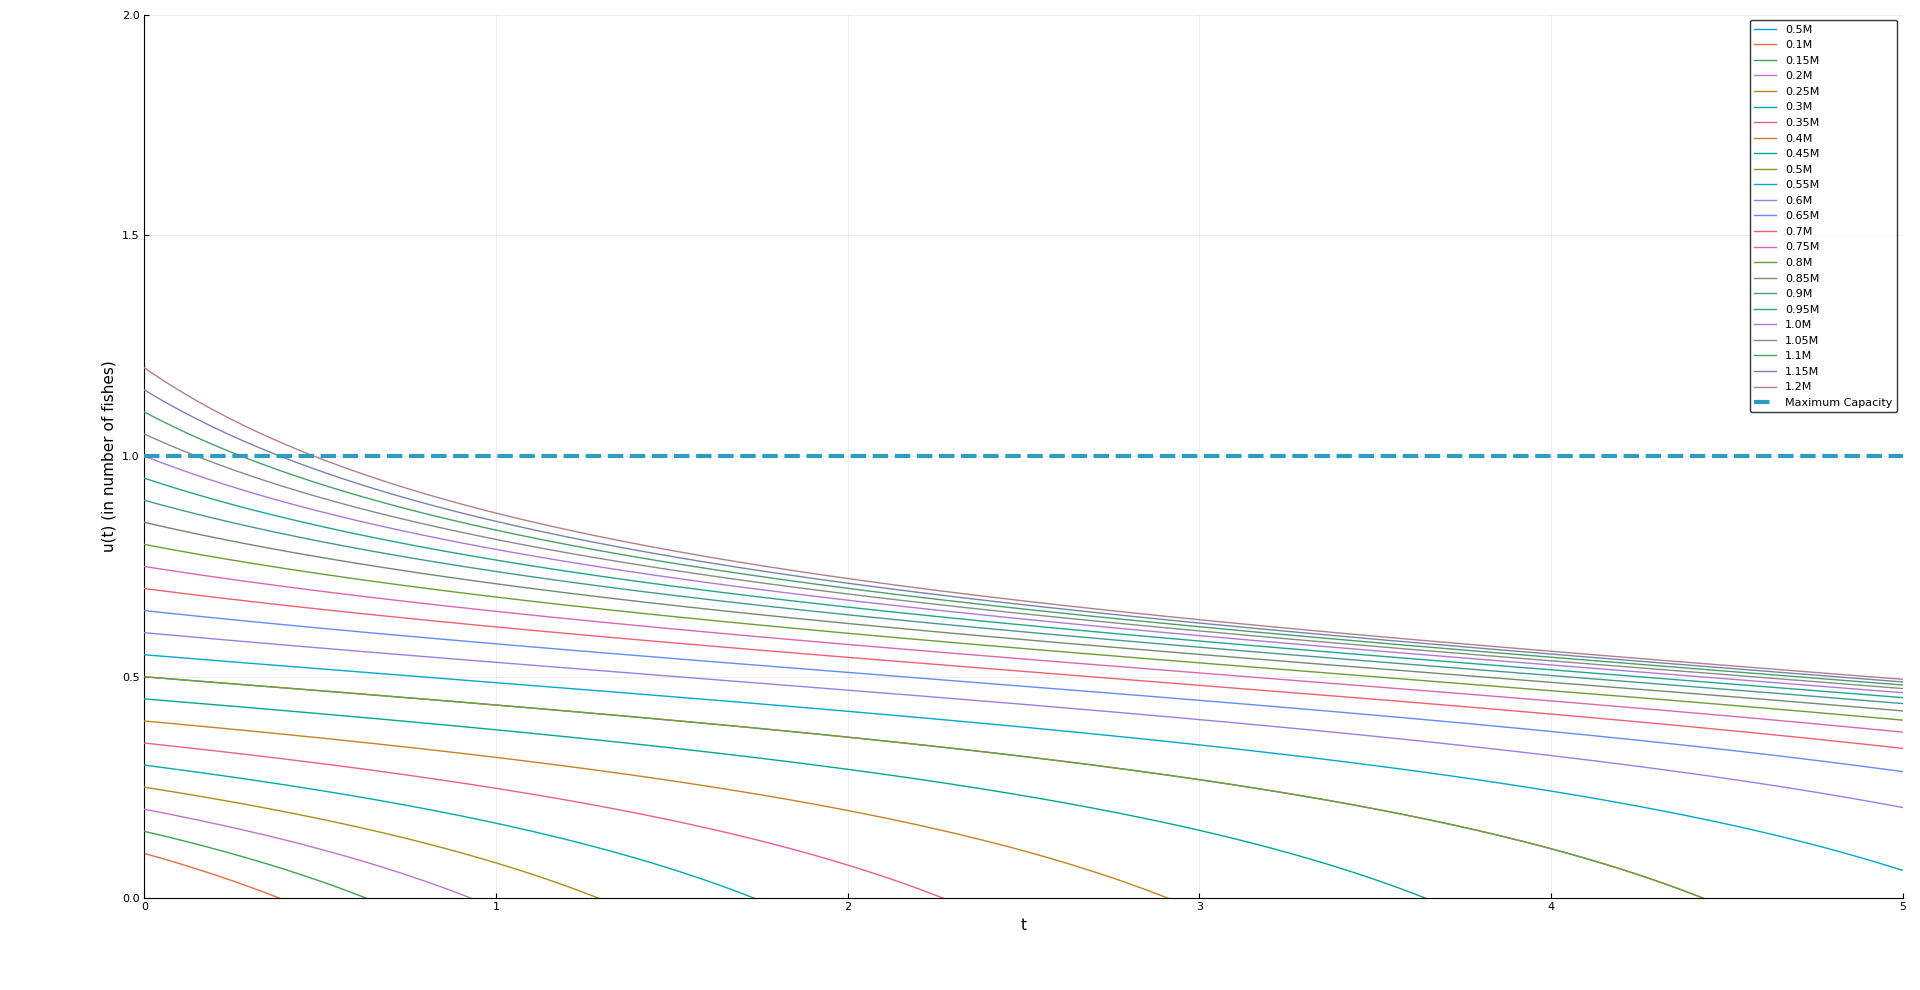
\includegraphics[width=0.8\textwidth]{OverExploitConstant.png}
	\caption{Constant harvest rate $u>\frac{rM}{4}$.}
	\label{fig: OverExploitConstantHarvest}
\end{figure}

\begin{figure}
	\centering
	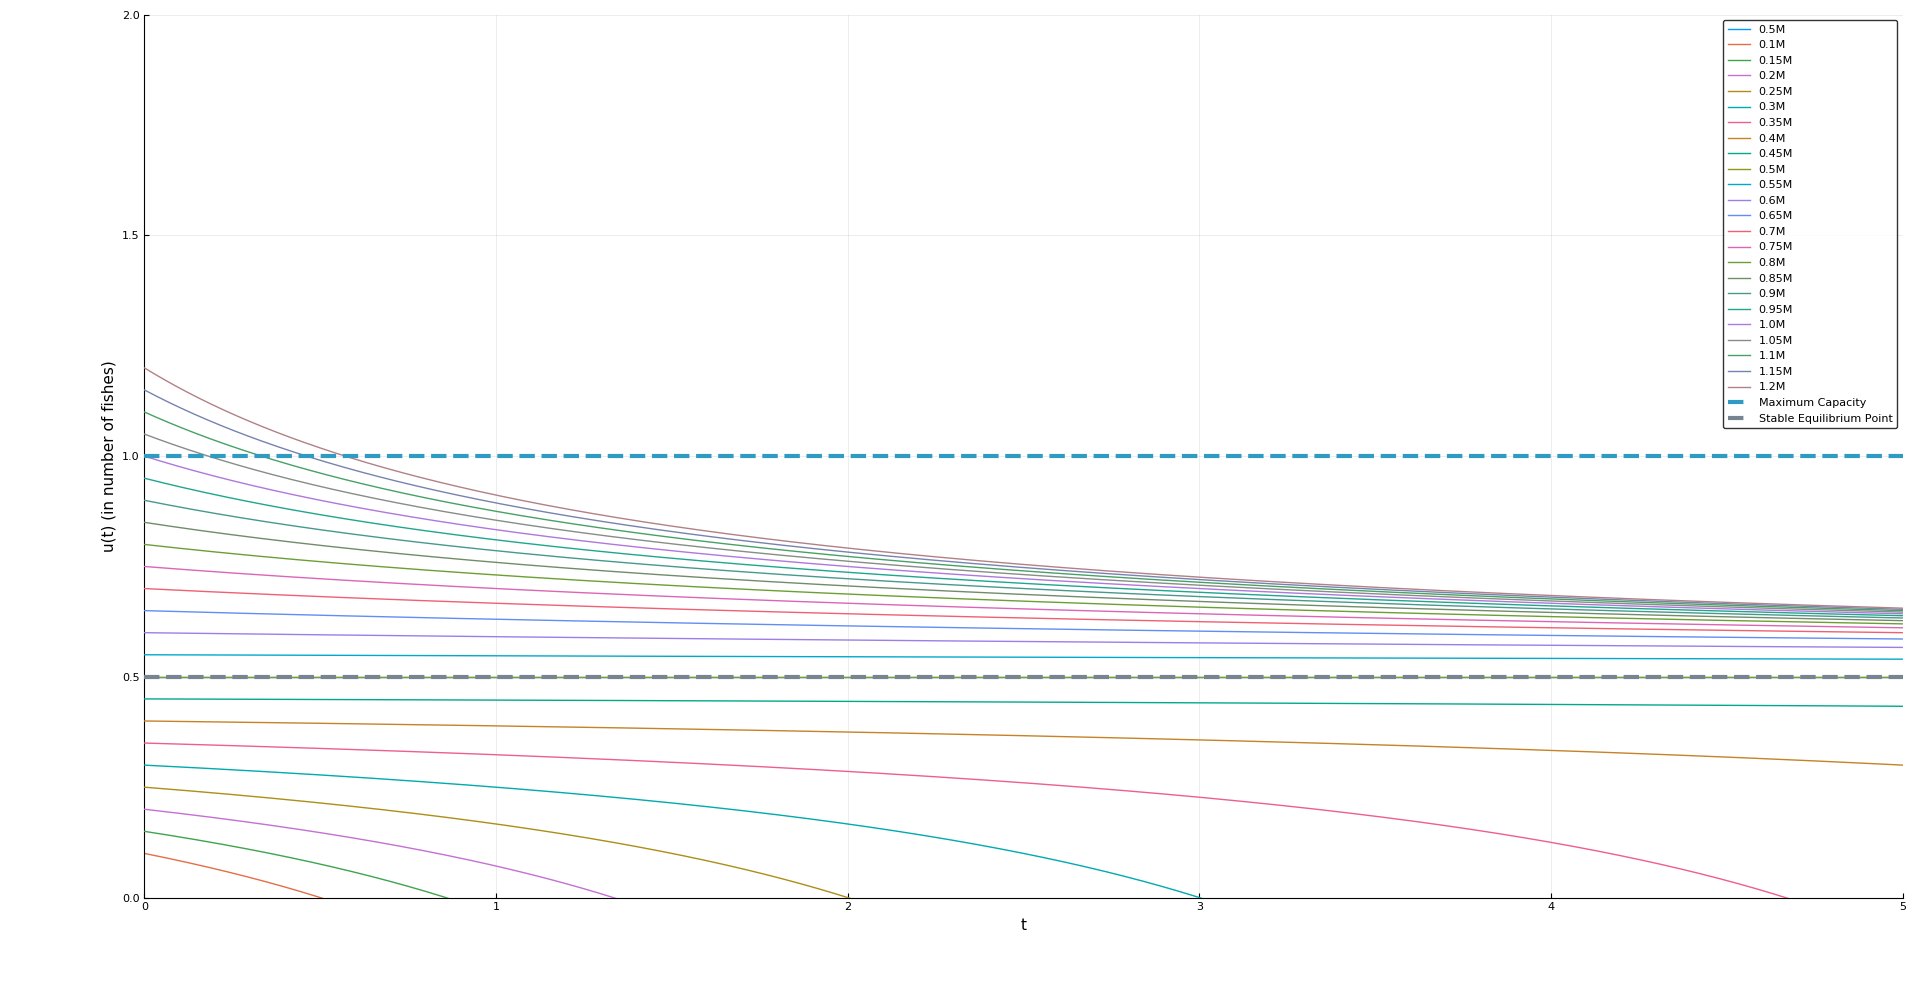
\includegraphics[width=0.8\textwidth]{CriticalExploitConstant.png}
	\caption{Constant harvest rate $u=\frac{rM}{4}$.}
	\label{fig: CriticalExploitConstantHarvest}
\end{figure}


\chapter{Mathematical Models.} \label{chap: Deterministic Model}
	\begin{equation}
\dev{x}{t}=rx\left(1-\frac{x}{M}\right)-u \label{eq: ConstantHarvest}
\end{equation}
We introduce the following variable in order to simply calculations,
\begin{equation}
\beta=\frac{uM}{r}
\end{equation}
Solving the differential equation,
\begin{align*}
	\frac{\diff{x}}{rx\left(1-\frac{x}{M}\right)-u}&=\diff{t} \\
	\int_{x_0}^{x}\frac{\diff{\chi}}{r\chi\left(1-\frac{\chi}{M}\right)-u}&=\int_{0}^{t}\diff{\tau} \\
	\frac{M}{r}\int_{x_0}^{x}\frac{\diff{\chi}}{\chi\left(M-\chi\right)-\frac{Mu}{r}}&=t \\
	-\frac{M}{r}\int_{x_0}^{x}\frac{\diff{\chi}}{\chi^2-M\chi+\beta}&=t \nonumber
	\end{align*}
Finally, we model the above integral as one 
\begin{align}
	-\frac{M}{r}\int_{x_0}^{x}\frac{\diff{\chi}}{\left(\chi-\frac{M}{2}\right)^2-\frac{M^2}{4}+\beta}&=t
\end{align}
Consider $\alpha$ as follows,
\begin{equation}
	\alpha = \beta - \frac{M^2}{4} = rM\left(u-\frac{rM}{4}\right)
\end{equation}
We see that the sign of $\alpha$ determines the nature of the solutions. Then, if $u>rM/4$ implies $\alpha>0$,
\begin{align*}
\int_{x_0}^{x}\frac{\diff{\chi}}{\left(\chi-\frac{M}{2}\right)^2+\alpha}&=-\frac{r}{M}t \\
\frac{1}{\sqrt{\beta-\frac{M^2}{4}}}\left(\arctan\left(\frac{x-M/2}{\sqrt{\beta-M^2/4}}\right)-\arctan\left(\frac{x_0-M/2}{\sqrt{\beta-M^2/4}}\right)\right)&=-\frac{r}{M}t \\
\end{align*}
Therefore, for $\alpha > 0$ the population behaves as follows, 
\begin{align}
	x(t)=\frac{M}{2}+\sqrt{\beta-\frac{M^2}{4}} \tan \left(\arctan\left(\frac{x_0-M/2}{\sqrt{\beta-M^2/4}}\right)-\frac{r\sqrt{\beta-M^2/4}}{M}t\right) \label{eq: ConstantHarvest OverExploit}
\end{align}

Equation \ref{eq: ConstantHarvest OverExploit} show us that for some $t^*$, $x(t^*)=0$,independently of the initial condition $x_0$, since the argument inside the $\tan$ is monotone decreasing in $t$. 

If $u<rM/4$ implies $-\alpha>0$,
\begin{align*}
	\int_{x_0}^{x}\frac{\diff{\chi}}{\left(\chi-\frac{M}{2}\right)^2-(-\alpha)} &=-\frac{r}{M}t
\end{align*}
Considering the zeros of the denominator, $\lambda$ and $\overleftarrow{\lambda}$, 
\begin{equation}
	\begin{array}{cc}
	\lambda&=\frac{M}{2}+\sqrt{\frac{M^2}{4}-\beta} \\
	\overline{\lambda}&=\frac{M}{2}-\sqrt{\frac{M^2}{4}-\beta} \\
	\end{array}
\end{equation}
We can rewrite our expression as follows, 
\begin{align*}
\int_{x_0}^{x} \left(\frac{1}{\chi - \lambda}-\frac{1}{\chi - \overline{\lambda}}\right)\diff{\chi} &=-\frac{2r\sqrt{M^2/4-\beta}}{M}t \\
	\ln\abs{\frac{x - \lambda}{x - \overline{\lambda}}}&=\ln\abs{\frac{x_0- \lambda}{x_0 - \overline{\lambda}}}-\frac{2r\sqrt{M^2/4-\beta}}{M}t
\end{align*}
For simplifying calculations, we write, $\gamma=\frac{2r\sqrt{M^2/4-\beta}}{M}$. And we obtain as result,
\begin{align}
\frac{x - \lambda}{x - \overline{\lambda}} &=\frac{x_0- \lambda}{x_0- \overline{\lambda}}\mathrm e^{-\gamma t} \\
x-\lambda &=\left(x-\overline{\lambda}\right)\left(\frac{x_0- \lambda}{x_0- \overline{\lambda}}\right)\mathrm e^{-\gamma t}
\end{align}

For the sake of simplicity, consider $\xi=\frac{x_0-\lambda}{x_0-\overline{\lambda}}\mathrm{e}^{-\gamma t}$. Therefore,
\begin{align*}
	x\left(1-\xi\right)&=\lambda-\overline{\lambda}\xi\\
	x&=\frac{\lambda-\overline{\lambda}\xi}{1-\xi} \\	
	x&=\frac{\frac{M}{2}+\sqrt{\frac{M^2}{4}-\beta}-\left(\frac{M}{2}-\sqrt{\frac{M^2}{4}-\beta}\right)\xi}{1-\xi}\\
	x&=\frac{\frac{M}{2}+\sqrt{\frac{M^2}{4}-\beta}-\left(\frac{M}{2}-\sqrt{\frac{M^2}{4}-\beta}\right)\xi}{1-\xi}\\
	x&=\frac{\frac{M}{2}\left(1-\xi\right)+\sqrt{\frac{M^2}{4}-\beta}\left(1+\xi\right)}{1-\xi}\\
	x&=\frac{M}{2}+\sqrt{\frac{M^2}{4}-\beta}\frac{1+\xi}{1-\xi}
\end{align*}
Hence, for $-\alpha>0$, we have the following result,
\begin{align}
	x(t)&=\frac{M}{2}+\left(\sqrt{\frac{M^2}{4}-\beta}\right)\frac{\left(x_0-M/2\right)\left(1+\mathrm e^{-\gamma t}\right)-\sqrt{M^2/4-\beta}\left(1-\mathrm{e}^{-\gamma t}\right)}{\left(x_0-M/2\right)\left(1-\mathrm e^{-\gamma t}\right)+\sqrt{M^2/4-\beta}\left(1+\mathrm{e}^{-\gamma t}\right)} \label{eq: Time Expression for Harvest}
\end{align}

If $u=\frac{rM}{4}$, we solve equation \ref{eq: ConstantHarvest} as follows,
\begin{align}
-\frac{M}{r}\int_{x_0}^{x}\frac{d\chi}{\left(\chi-\frac{M}{2}\right)^2}&=t\\
\int_{x_0}^{x}\frac{d\chi}{\left(\chi-\frac{M}{2}\right)^2}&=-\frac{rt}{M}\\
\frac{1}{x-\frac{M}{2}}&=\frac{1}{x_0-\frac{M}{2}}-\frac{rt}{M}\\
\frac{1}{x-\frac{M}{2}}&=\frac{M-\left(x_0-\frac{M}{2}\right)rt}{M\left(x_0-\frac{M}{2}\right)} \\
x&=\frac{M}{2}+\frac{M\left(x_0-\frac{M}{2}\right)}{M-\left(x_0-\frac{M}{2}\right)rt} 
\end{align}

The results above stated can be explained directly from the equation \ref{eq: ConstantHarvest}, as we see in the graph \ref{fig: CriticalPoints},  $F(x,t)$ is a paraboloid, with its maximum at $F(x^*=M/2,t)=rM^2/4$.

When $u=0$, we have the regular logistic equation with critical points $x_{c_1}=0$ and $x_{c_2}=M$. With $x_{c_2}$ being an stable fixed point and $x_{c_1}$ an unstable fixed point. In general, these are the solutions to the equation $F(x,t)-u=0$,
\begin{equation}
x_{c_{2,1}}=\frac{M}{2}\pm \sqrt{\frac{M^2}{4}-u\frac{M}{r}}
\end{equation}

We observe that the critical points $x_c$, such that $\dev{x_c}{t}=F(x_c, t)-u=0$ are getting closer to each other, as $u$ is increasing; when $u=\frac{rM}{4}$ we only have one critical unstable point. That behaves as an attractor when $x_0\geq\frac{M}{2}$. But when $x_0<\frac{M}{2}$ the population strictly decreases. For $u> \frac{rM}{4}$, the population $x(t)$ has no real critical points and the derivative $\dev{x}{t}$ is always negative, implying, that we will lead always the population to extinction, extracting constantly at a rate greater than $\frac{rM}{4}$.

\begin{figure}[H]
	\centering
	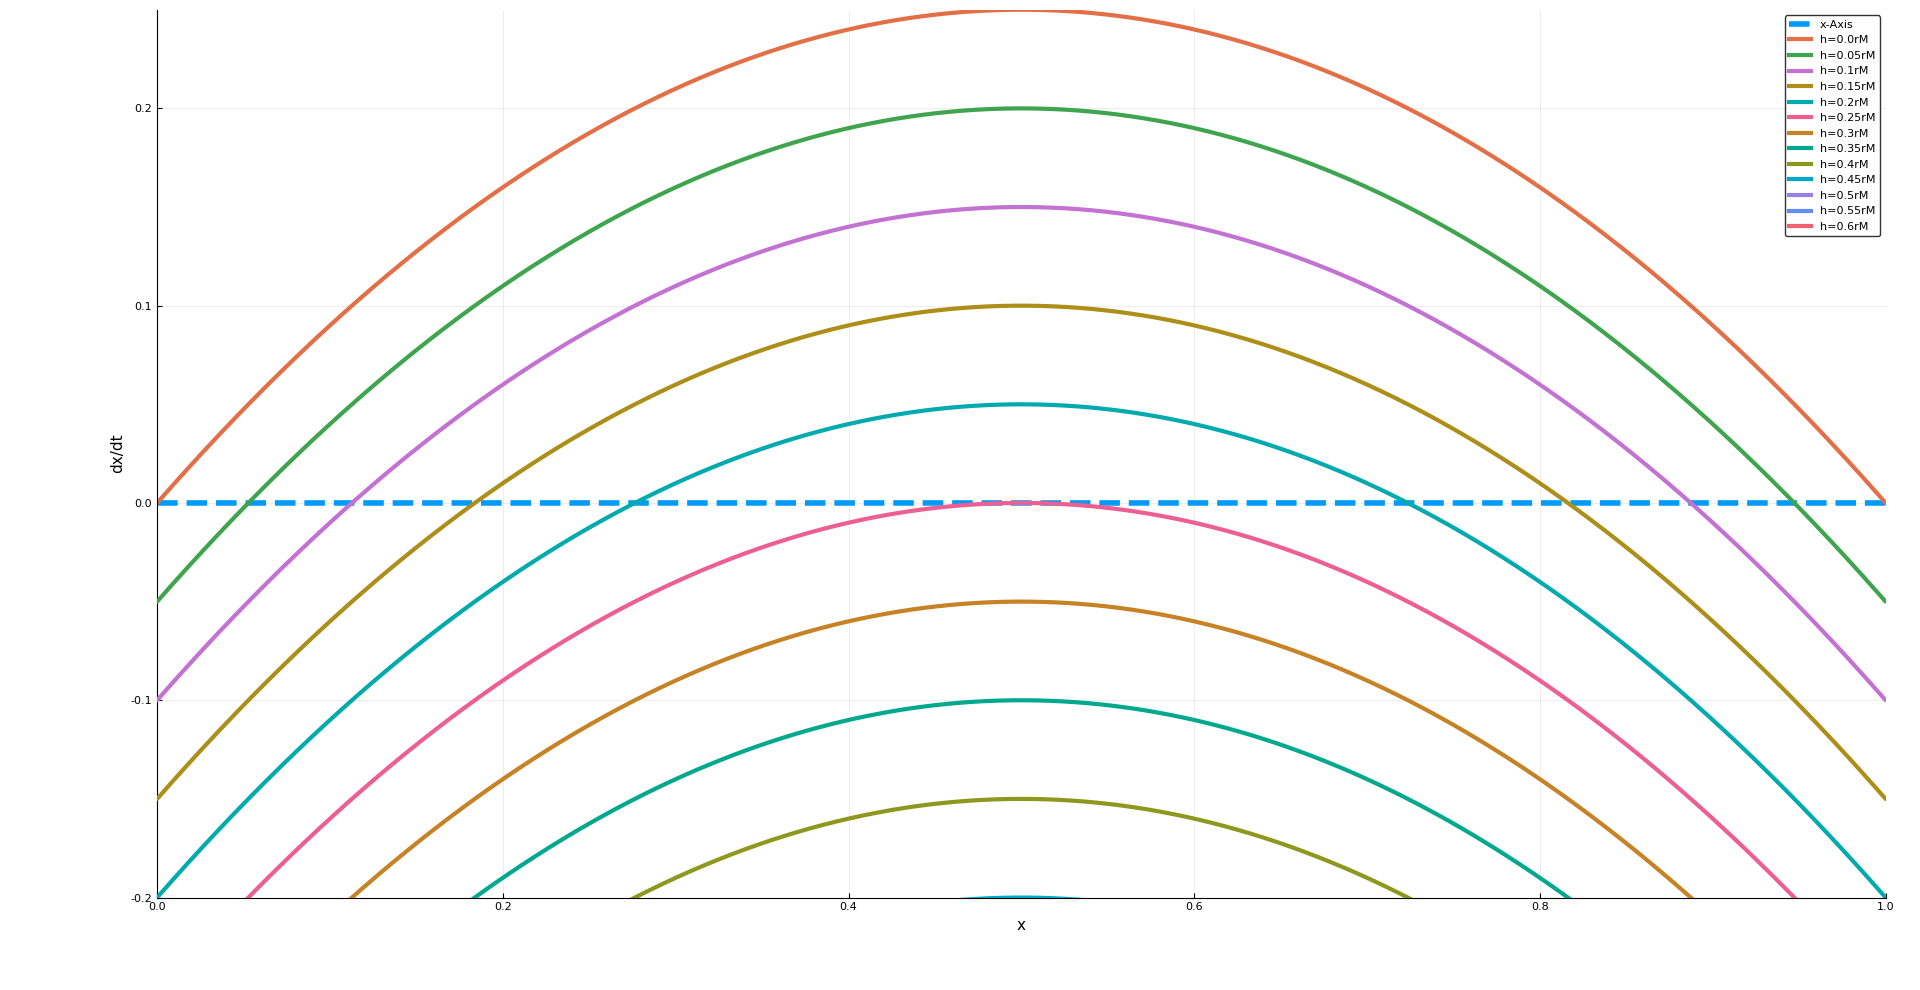
\includegraphics[width=0.8\textwidth]{CriticalPoints.png}
	\caption{Figure representing $\dev{x}{t}$ with different harvesting rates.}
	\label{fig: CriticalPoints}
\end{figure}
\begin{figure}
		\centering
		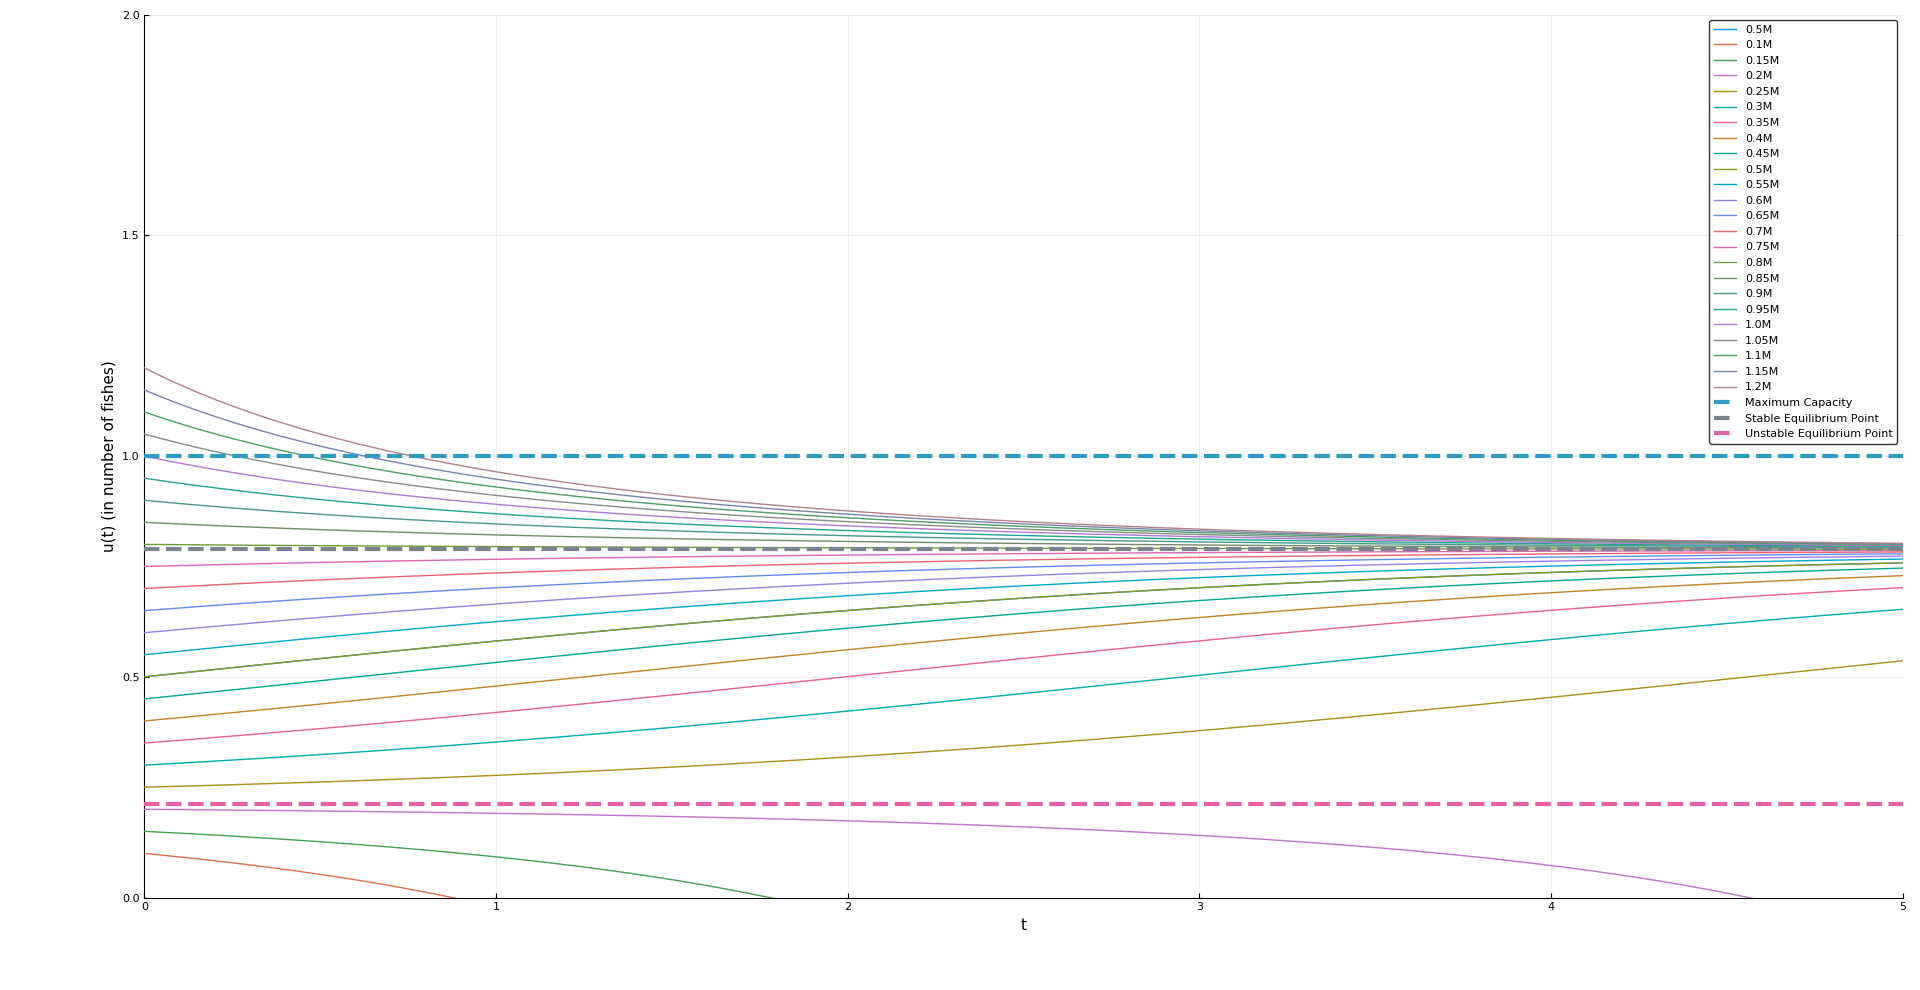
\includegraphics[width=0.8\textwidth]{SustainableConstant.png}
		\caption{Constant harvest rate $u<\frac{rM}{4}$.}
		\label{fig: SustainableConstantHarvest}
\end{figure}
\begin{figure}
	\centering
	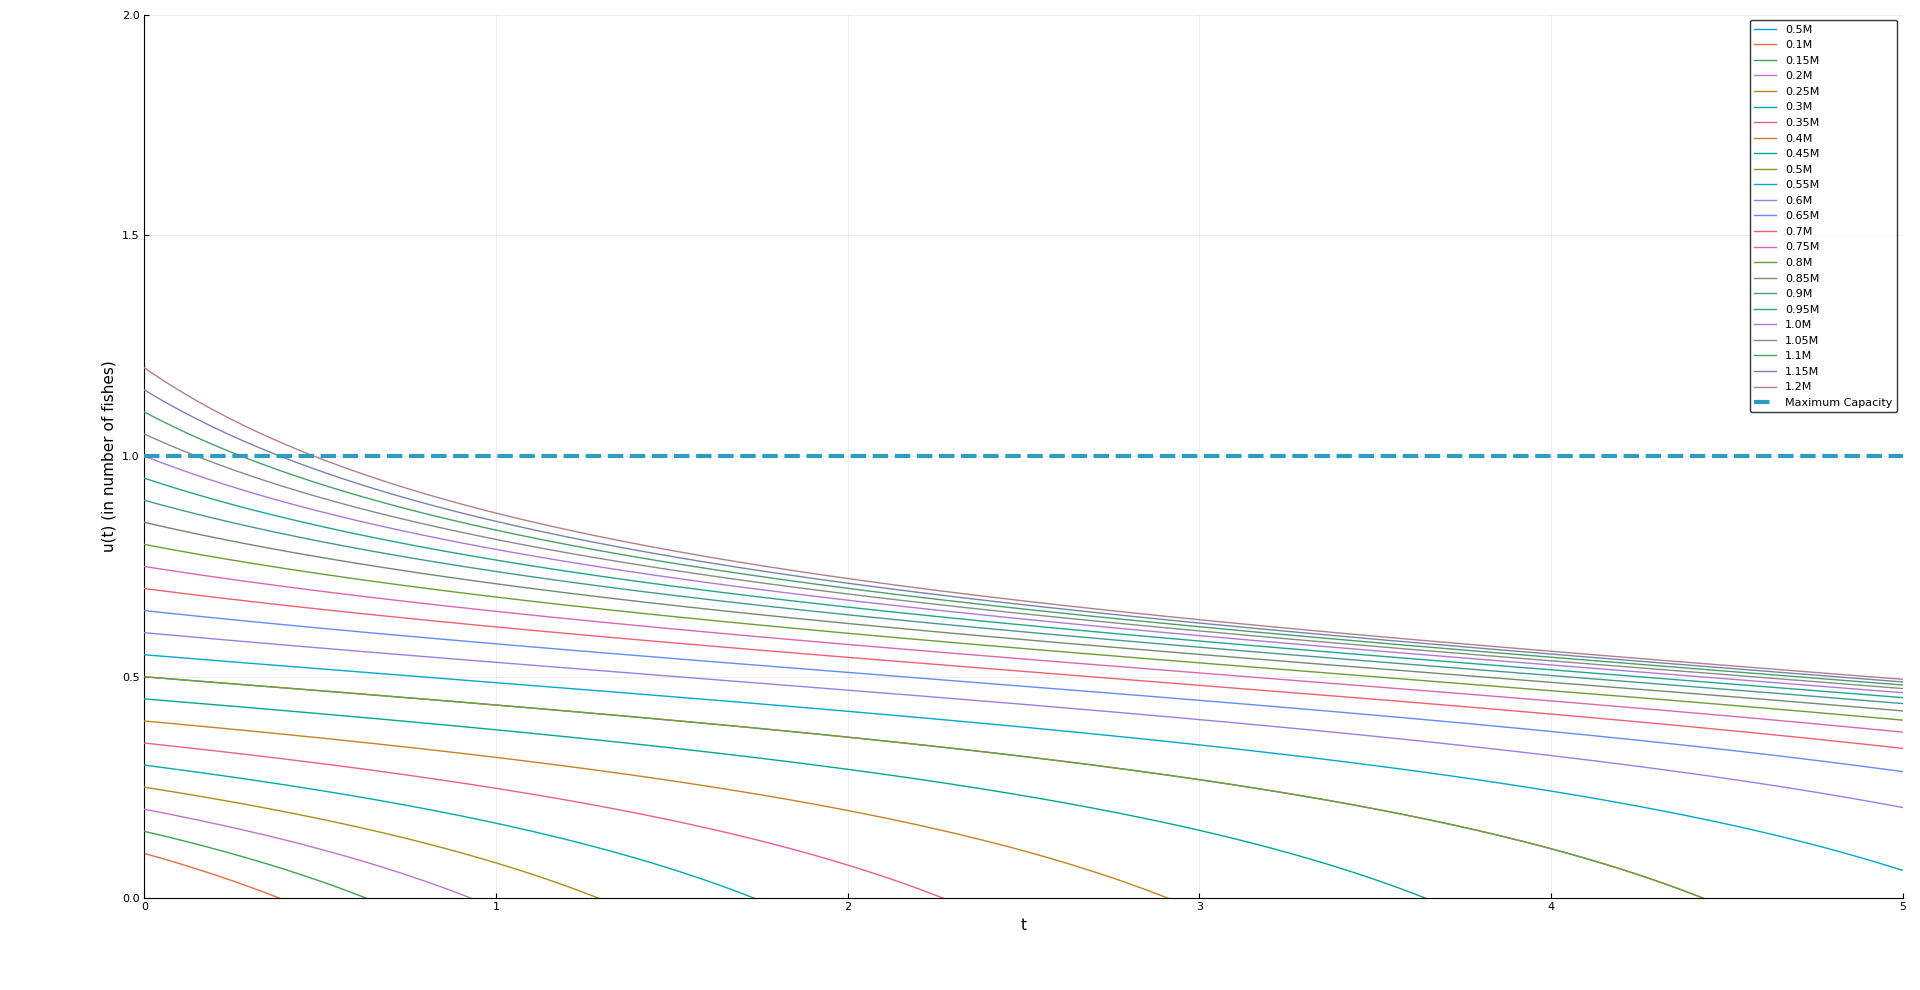
\includegraphics[width=0.8\textwidth]{OverExploitConstant.png}
	\caption{Constant harvest rate $u>\frac{rM}{4}$.}
	\label{fig: OverExploitConstantHarvest}
\end{figure}

\begin{figure}
	\centering
	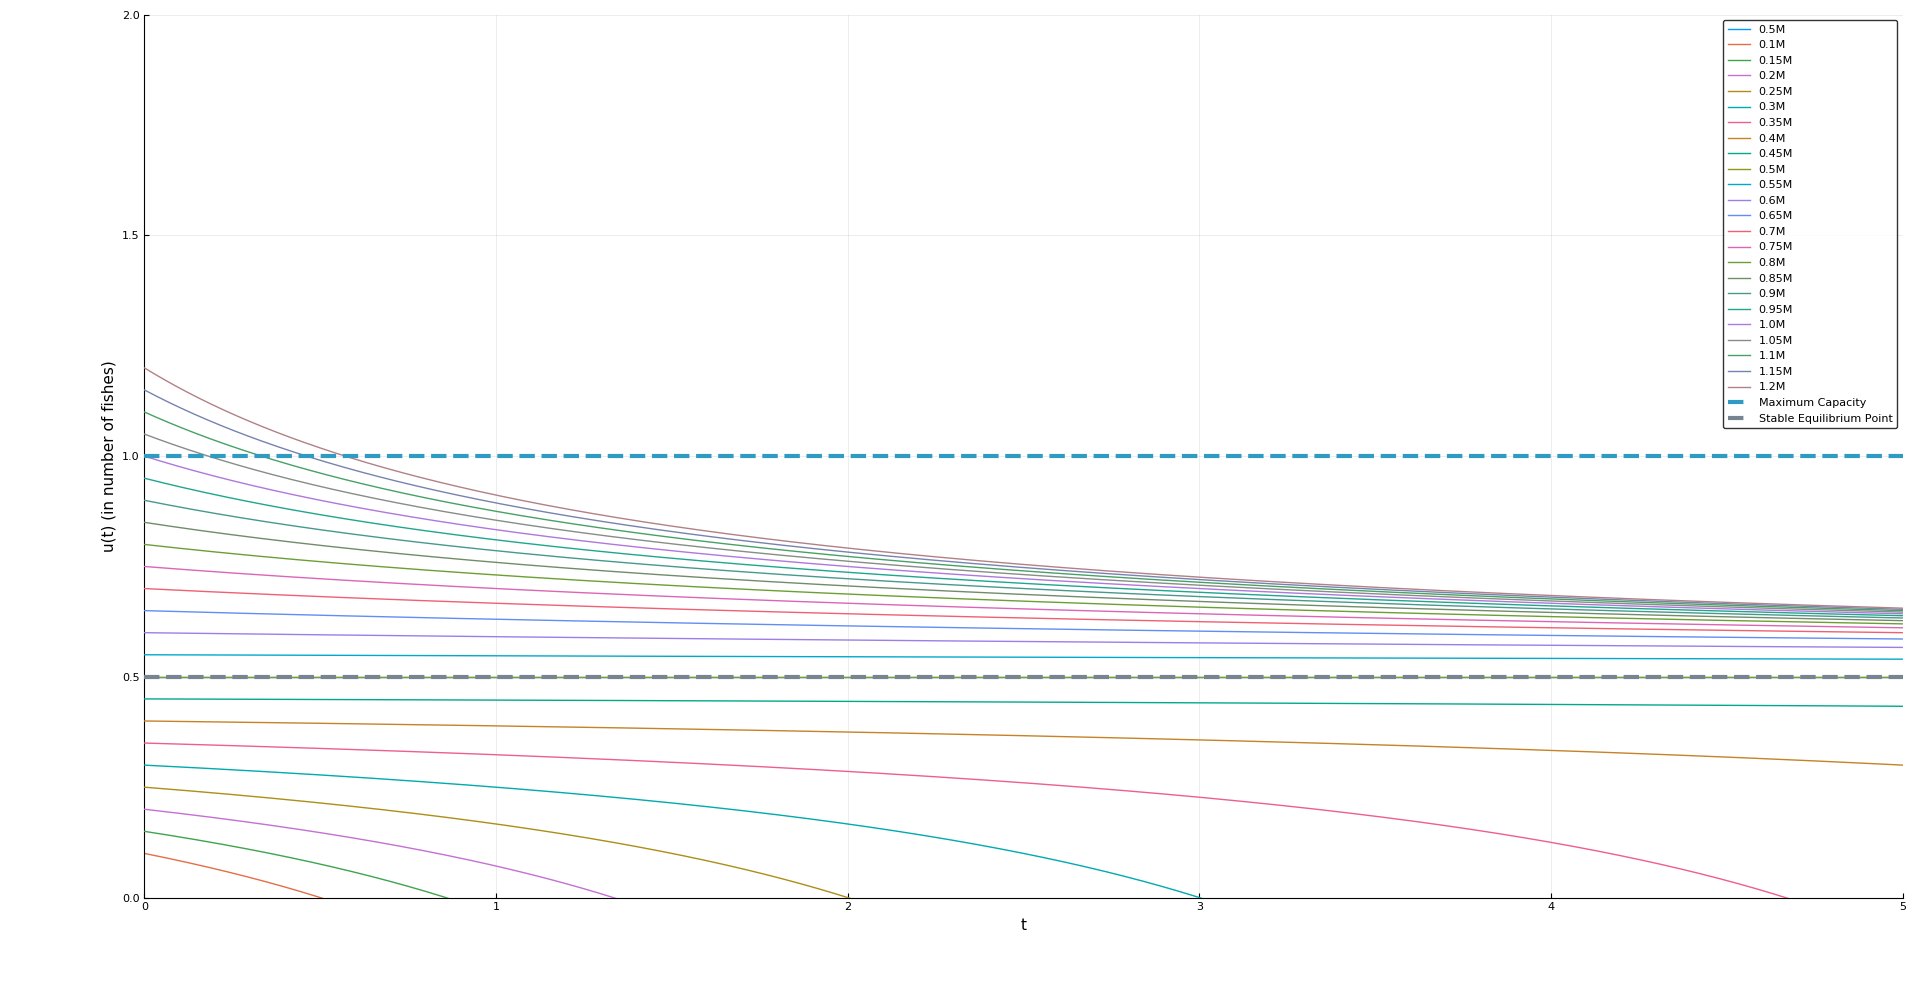
\includegraphics[width=0.8\textwidth]{CriticalExploitConstant.png}
	\caption{Constant harvest rate $u=\frac{rM}{4}$.}
	\label{fig: CriticalExploitConstantHarvest}
\end{figure}


	\section{Exponential biological growth.}
		\graphicspath{{Model/ExponentialGrowth/}}
		\begin{equation}
\dev{x}{t}=rx\left(1-\frac{x}{M}\right)-u \label{eq: ConstantHarvest}
\end{equation}
We introduce the following variable in order to simply calculations,
\begin{equation}
\beta=\frac{uM}{r}
\end{equation}
Solving the differential equation,
\begin{align*}
	\frac{\diff{x}}{rx\left(1-\frac{x}{M}\right)-u}&=\diff{t} \\
	\int_{x_0}^{x}\frac{\diff{\chi}}{r\chi\left(1-\frac{\chi}{M}\right)-u}&=\int_{0}^{t}\diff{\tau} \\
	\frac{M}{r}\int_{x_0}^{x}\frac{\diff{\chi}}{\chi\left(M-\chi\right)-\frac{Mu}{r}}&=t \\
	-\frac{M}{r}\int_{x_0}^{x}\frac{\diff{\chi}}{\chi^2-M\chi+\beta}&=t \nonumber
	\end{align*}
Finally, we model the above integral as one 
\begin{align}
	-\frac{M}{r}\int_{x_0}^{x}\frac{\diff{\chi}}{\left(\chi-\frac{M}{2}\right)^2-\frac{M^2}{4}+\beta}&=t
\end{align}
Consider $\alpha$ as follows,
\begin{equation}
	\alpha = \beta - \frac{M^2}{4} = rM\left(u-\frac{rM}{4}\right)
\end{equation}
We see that the sign of $\alpha$ determines the nature of the solutions. Then, if $u>rM/4$ implies $\alpha>0$,
\begin{align*}
\int_{x_0}^{x}\frac{\diff{\chi}}{\left(\chi-\frac{M}{2}\right)^2+\alpha}&=-\frac{r}{M}t \\
\frac{1}{\sqrt{\beta-\frac{M^2}{4}}}\left(\arctan\left(\frac{x-M/2}{\sqrt{\beta-M^2/4}}\right)-\arctan\left(\frac{x_0-M/2}{\sqrt{\beta-M^2/4}}\right)\right)&=-\frac{r}{M}t \\
\end{align*}
Therefore, for $\alpha > 0$ the population behaves as follows, 
\begin{align}
	x(t)=\frac{M}{2}+\sqrt{\beta-\frac{M^2}{4}} \tan \left(\arctan\left(\frac{x_0-M/2}{\sqrt{\beta-M^2/4}}\right)-\frac{r\sqrt{\beta-M^2/4}}{M}t\right) \label{eq: ConstantHarvest OverExploit}
\end{align}

Equation \ref{eq: ConstantHarvest OverExploit} show us that for some $t^*$, $x(t^*)=0$,independently of the initial condition $x_0$, since the argument inside the $\tan$ is monotone decreasing in $t$. 

If $u<rM/4$ implies $-\alpha>0$,
\begin{align*}
	\int_{x_0}^{x}\frac{\diff{\chi}}{\left(\chi-\frac{M}{2}\right)^2-(-\alpha)} &=-\frac{r}{M}t
\end{align*}
Considering the zeros of the denominator, $\lambda$ and $\overleftarrow{\lambda}$, 
\begin{equation}
	\begin{array}{cc}
	\lambda&=\frac{M}{2}+\sqrt{\frac{M^2}{4}-\beta} \\
	\overline{\lambda}&=\frac{M}{2}-\sqrt{\frac{M^2}{4}-\beta} \\
	\end{array}
\end{equation}
We can rewrite our expression as follows, 
\begin{align*}
\int_{x_0}^{x} \left(\frac{1}{\chi - \lambda}-\frac{1}{\chi - \overline{\lambda}}\right)\diff{\chi} &=-\frac{2r\sqrt{M^2/4-\beta}}{M}t \\
	\ln\abs{\frac{x - \lambda}{x - \overline{\lambda}}}&=\ln\abs{\frac{x_0- \lambda}{x_0 - \overline{\lambda}}}-\frac{2r\sqrt{M^2/4-\beta}}{M}t
\end{align*}
For simplifying calculations, we write, $\gamma=\frac{2r\sqrt{M^2/4-\beta}}{M}$. And we obtain as result,
\begin{align}
\frac{x - \lambda}{x - \overline{\lambda}} &=\frac{x_0- \lambda}{x_0- \overline{\lambda}}\mathrm e^{-\gamma t} \\
x-\lambda &=\left(x-\overline{\lambda}\right)\left(\frac{x_0- \lambda}{x_0- \overline{\lambda}}\right)\mathrm e^{-\gamma t}
\end{align}

For the sake of simplicity, consider $\xi=\frac{x_0-\lambda}{x_0-\overline{\lambda}}\mathrm{e}^{-\gamma t}$. Therefore,
\begin{align*}
	x\left(1-\xi\right)&=\lambda-\overline{\lambda}\xi\\
	x&=\frac{\lambda-\overline{\lambda}\xi}{1-\xi} \\	
	x&=\frac{\frac{M}{2}+\sqrt{\frac{M^2}{4}-\beta}-\left(\frac{M}{2}-\sqrt{\frac{M^2}{4}-\beta}\right)\xi}{1-\xi}\\
	x&=\frac{\frac{M}{2}+\sqrt{\frac{M^2}{4}-\beta}-\left(\frac{M}{2}-\sqrt{\frac{M^2}{4}-\beta}\right)\xi}{1-\xi}\\
	x&=\frac{\frac{M}{2}\left(1-\xi\right)+\sqrt{\frac{M^2}{4}-\beta}\left(1+\xi\right)}{1-\xi}\\
	x&=\frac{M}{2}+\sqrt{\frac{M^2}{4}-\beta}\frac{1+\xi}{1-\xi}
\end{align*}
Hence, for $-\alpha>0$, we have the following result,
\begin{align}
	x(t)&=\frac{M}{2}+\left(\sqrt{\frac{M^2}{4}-\beta}\right)\frac{\left(x_0-M/2\right)\left(1+\mathrm e^{-\gamma t}\right)-\sqrt{M^2/4-\beta}\left(1-\mathrm{e}^{-\gamma t}\right)}{\left(x_0-M/2\right)\left(1-\mathrm e^{-\gamma t}\right)+\sqrt{M^2/4-\beta}\left(1+\mathrm{e}^{-\gamma t}\right)} \label{eq: Time Expression for Harvest}
\end{align}

If $u=\frac{rM}{4}$, we solve equation \ref{eq: ConstantHarvest} as follows,
\begin{align}
-\frac{M}{r}\int_{x_0}^{x}\frac{d\chi}{\left(\chi-\frac{M}{2}\right)^2}&=t\\
\int_{x_0}^{x}\frac{d\chi}{\left(\chi-\frac{M}{2}\right)^2}&=-\frac{rt}{M}\\
\frac{1}{x-\frac{M}{2}}&=\frac{1}{x_0-\frac{M}{2}}-\frac{rt}{M}\\
\frac{1}{x-\frac{M}{2}}&=\frac{M-\left(x_0-\frac{M}{2}\right)rt}{M\left(x_0-\frac{M}{2}\right)} \\
x&=\frac{M}{2}+\frac{M\left(x_0-\frac{M}{2}\right)}{M-\left(x_0-\frac{M}{2}\right)rt} 
\end{align}

The results above stated can be explained directly from the equation \ref{eq: ConstantHarvest}, as we see in the graph \ref{fig: CriticalPoints},  $F(x,t)$ is a paraboloid, with its maximum at $F(x^*=M/2,t)=rM^2/4$.

When $u=0$, we have the regular logistic equation with critical points $x_{c_1}=0$ and $x_{c_2}=M$. With $x_{c_2}$ being an stable fixed point and $x_{c_1}$ an unstable fixed point. In general, these are the solutions to the equation $F(x,t)-u=0$,
\begin{equation}
x_{c_{2,1}}=\frac{M}{2}\pm \sqrt{\frac{M^2}{4}-u\frac{M}{r}}
\end{equation}

We observe that the critical points $x_c$, such that $\dev{x_c}{t}=F(x_c, t)-u=0$ are getting closer to each other, as $u$ is increasing; when $u=\frac{rM}{4}$ we only have one critical unstable point. That behaves as an attractor when $x_0\geq\frac{M}{2}$. But when $x_0<\frac{M}{2}$ the population strictly decreases. For $u> \frac{rM}{4}$, the population $x(t)$ has no real critical points and the derivative $\dev{x}{t}$ is always negative, implying, that we will lead always the population to extinction, extracting constantly at a rate greater than $\frac{rM}{4}$.

\begin{figure}[H]
	\centering
	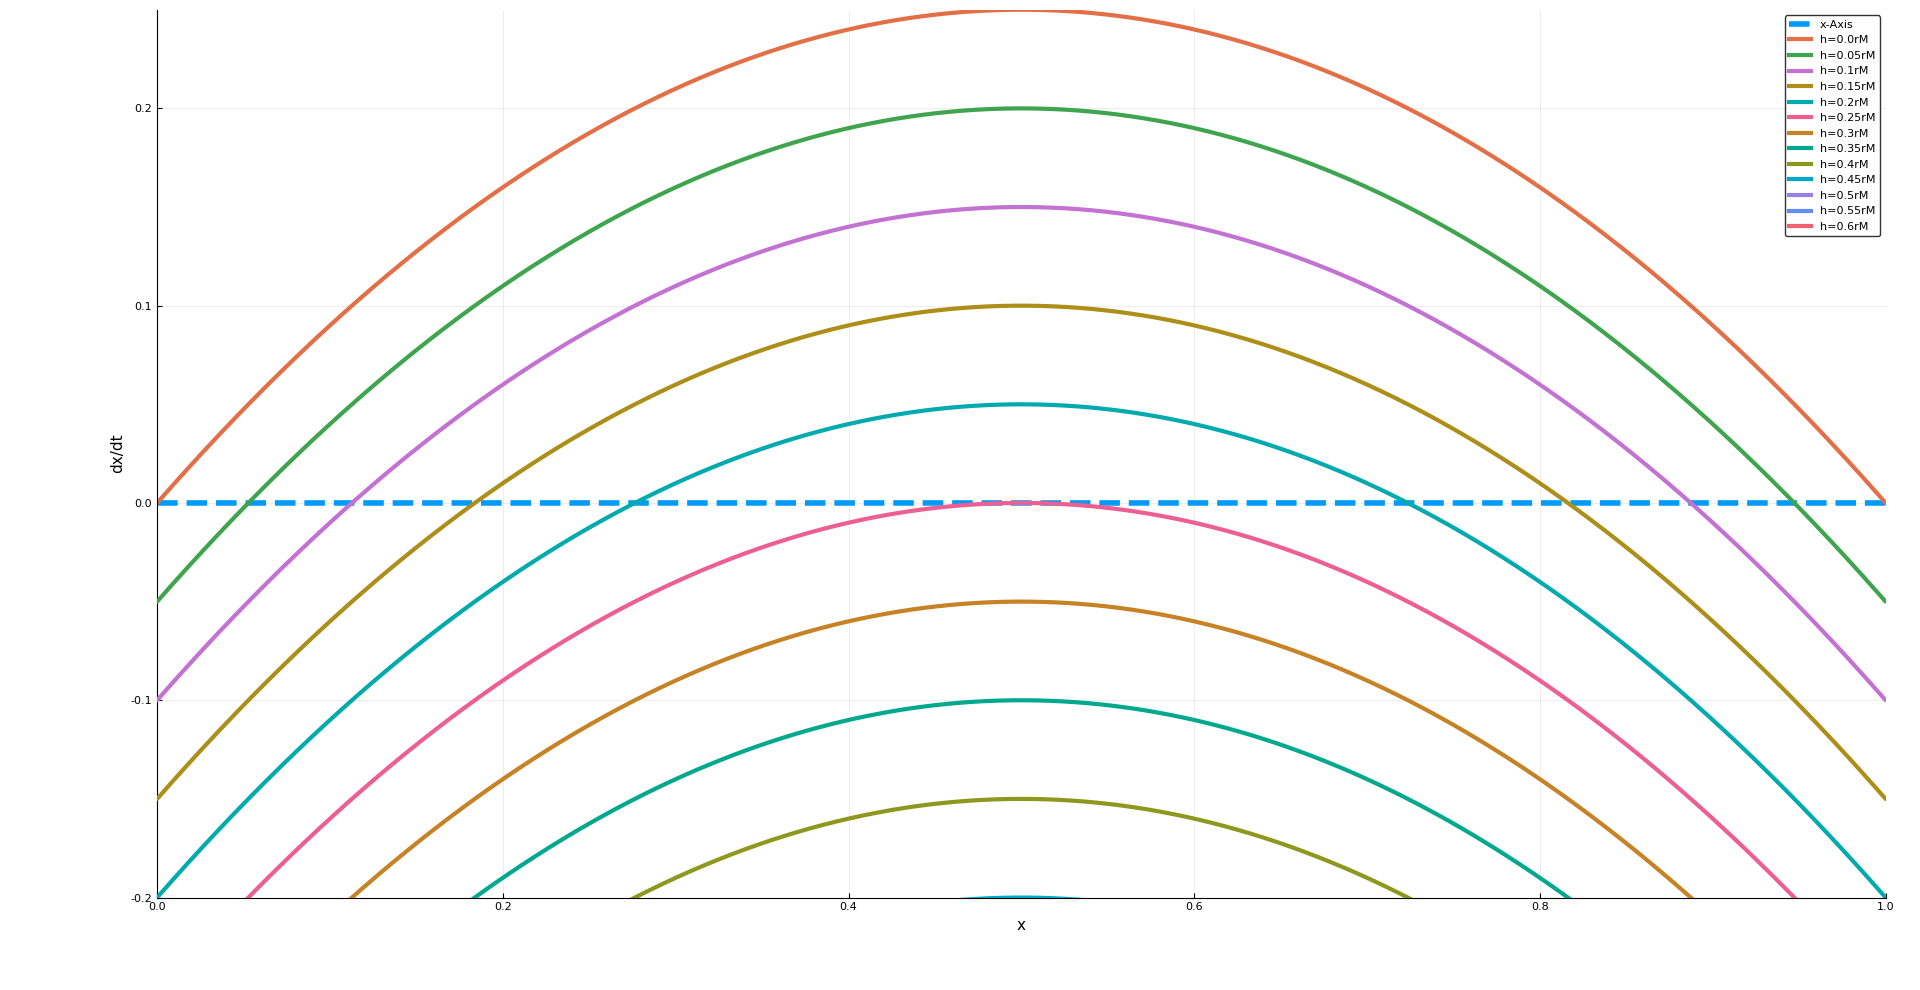
\includegraphics[width=0.8\textwidth]{CriticalPoints.png}
	\caption{Figure representing $\dev{x}{t}$ with different harvesting rates.}
	\label{fig: CriticalPoints}
\end{figure}
\begin{figure}
		\centering
		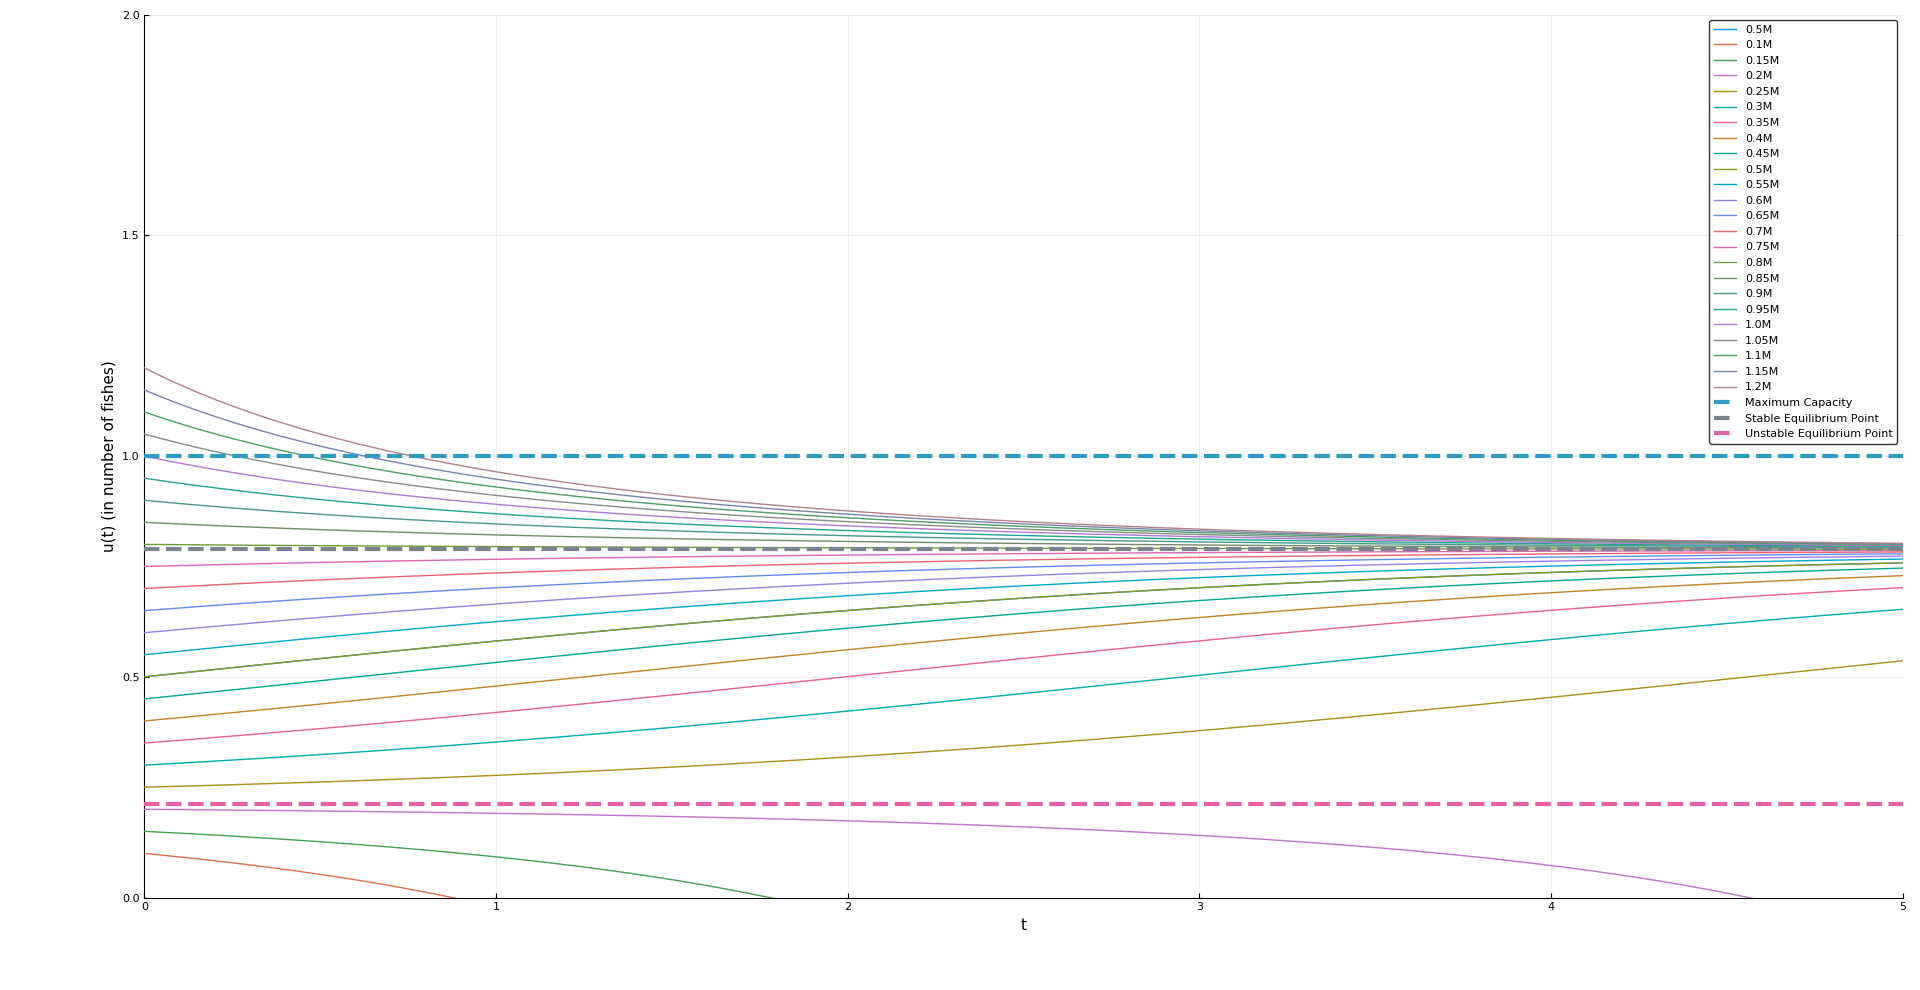
\includegraphics[width=0.8\textwidth]{SustainableConstant.png}
		\caption{Constant harvest rate $u<\frac{rM}{4}$.}
		\label{fig: SustainableConstantHarvest}
\end{figure}
\begin{figure}
	\centering
	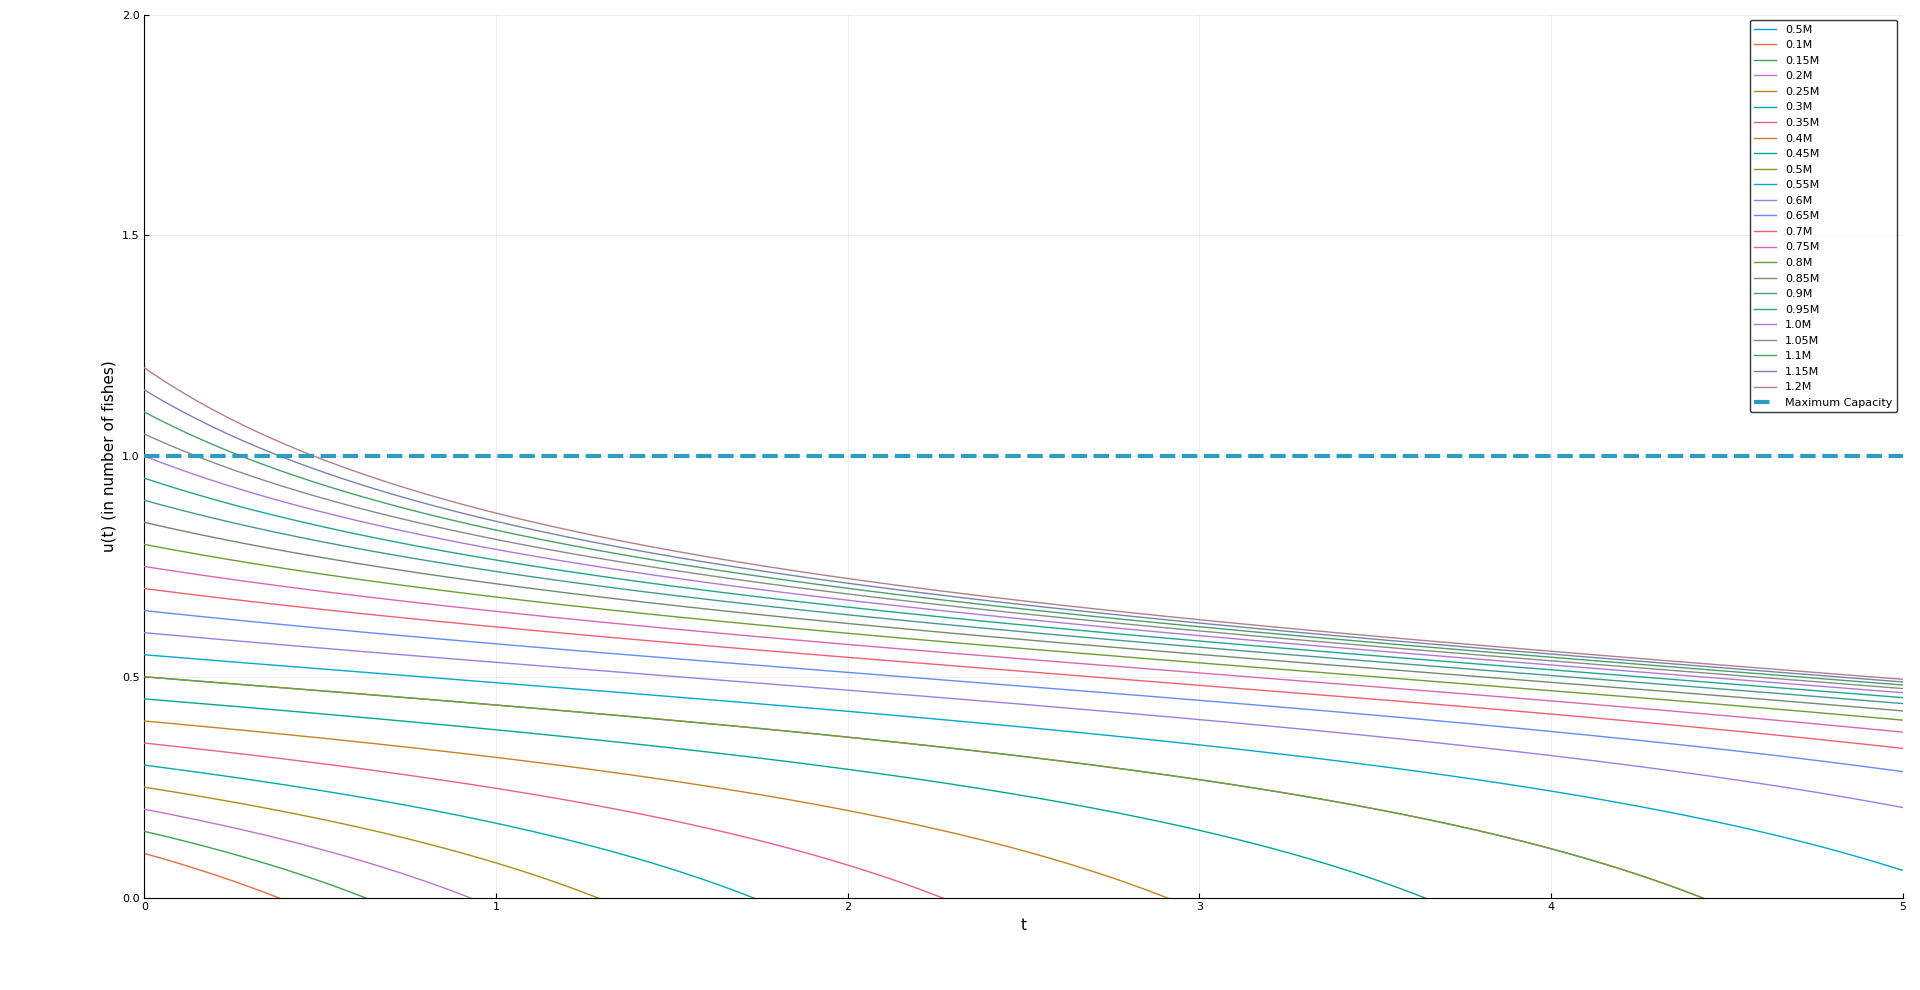
\includegraphics[width=0.8\textwidth]{OverExploitConstant.png}
	\caption{Constant harvest rate $u>\frac{rM}{4}$.}
	\label{fig: OverExploitConstantHarvest}
\end{figure}

\begin{figure}
	\centering
	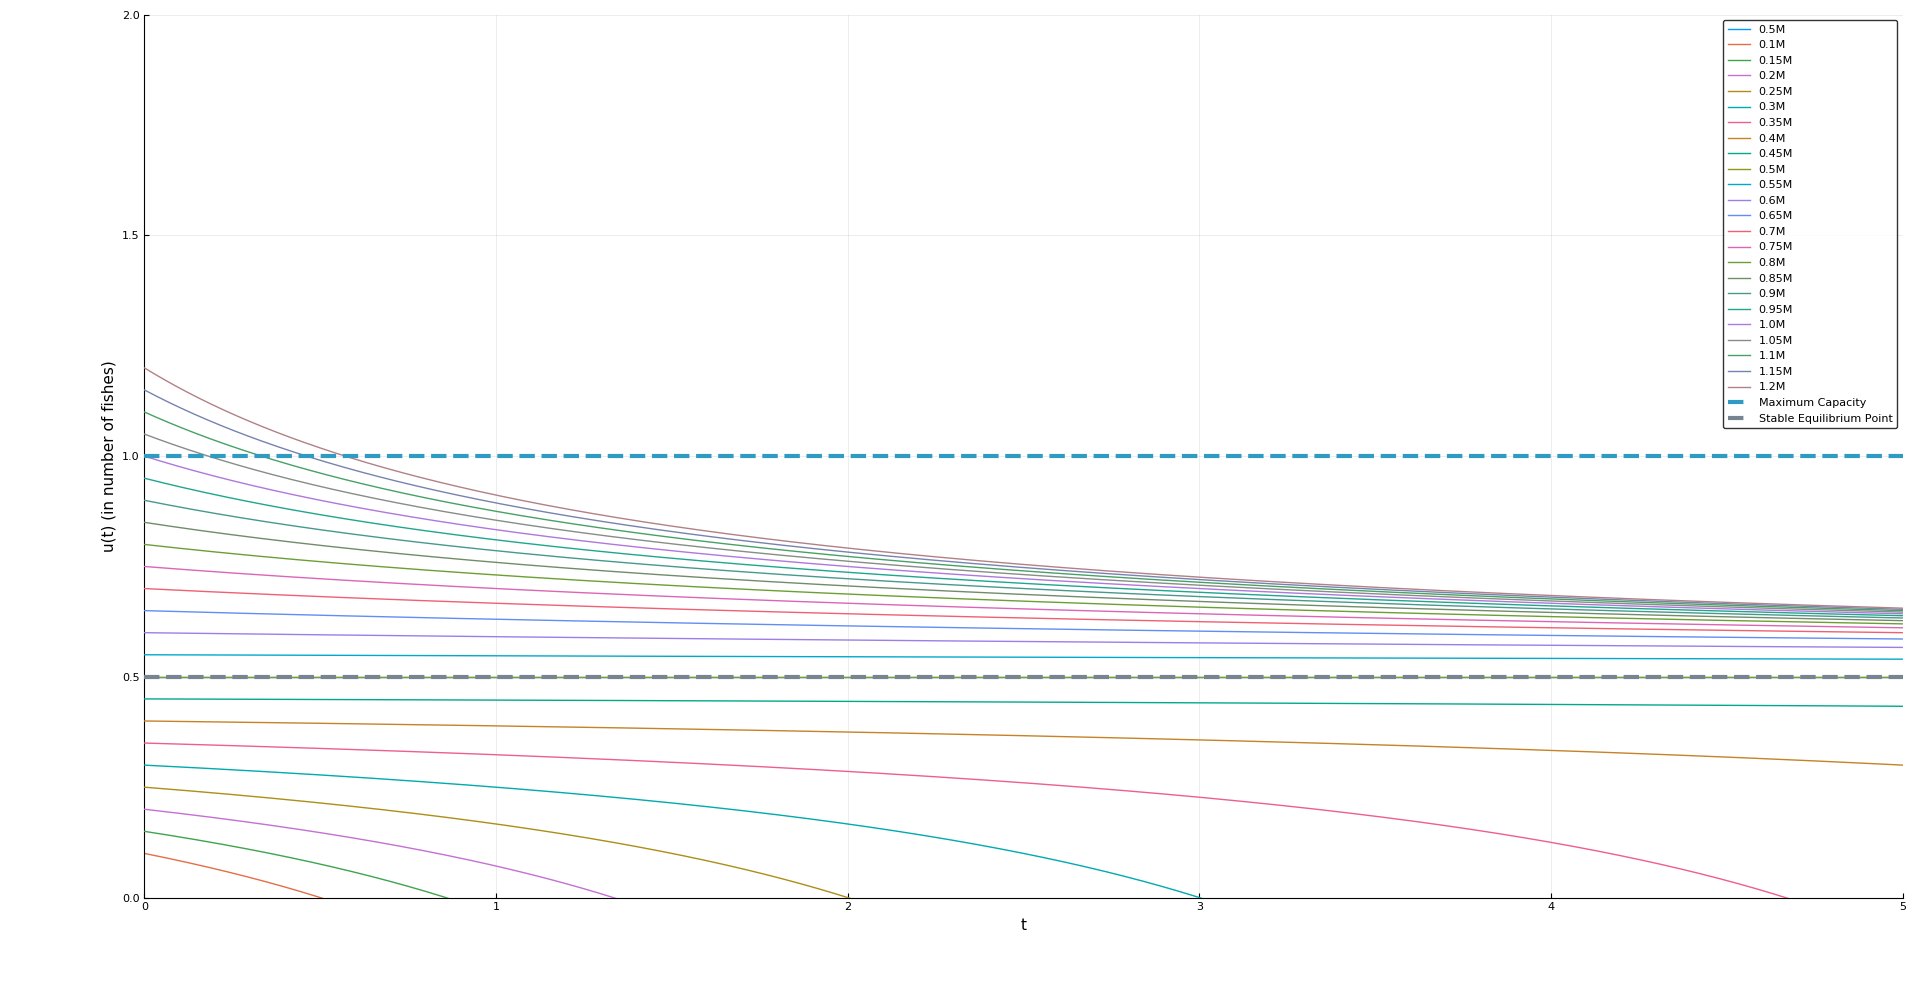
\includegraphics[width=0.8\textwidth]{CriticalExploitConstant.png}
	\caption{Constant harvest rate $u=\frac{rM}{4}$.}
	\label{fig: CriticalExploitConstantHarvest}
\end{figure}


	\section{Logistic Equation.}
		\graphicspath{{Model/LogisticEquation/}}
		\begin{equation}
\dev{x}{t}=rx\left(1-\frac{x}{M}\right)-u \label{eq: ConstantHarvest}
\end{equation}
We introduce the following variable in order to simply calculations,
\begin{equation}
\beta=\frac{uM}{r}
\end{equation}
Solving the differential equation,
\begin{align*}
	\frac{\diff{x}}{rx\left(1-\frac{x}{M}\right)-u}&=\diff{t} \\
	\int_{x_0}^{x}\frac{\diff{\chi}}{r\chi\left(1-\frac{\chi}{M}\right)-u}&=\int_{0}^{t}\diff{\tau} \\
	\frac{M}{r}\int_{x_0}^{x}\frac{\diff{\chi}}{\chi\left(M-\chi\right)-\frac{Mu}{r}}&=t \\
	-\frac{M}{r}\int_{x_0}^{x}\frac{\diff{\chi}}{\chi^2-M\chi+\beta}&=t \nonumber
	\end{align*}
Finally, we model the above integral as one 
\begin{align}
	-\frac{M}{r}\int_{x_0}^{x}\frac{\diff{\chi}}{\left(\chi-\frac{M}{2}\right)^2-\frac{M^2}{4}+\beta}&=t
\end{align}
Consider $\alpha$ as follows,
\begin{equation}
	\alpha = \beta - \frac{M^2}{4} = rM\left(u-\frac{rM}{4}\right)
\end{equation}
We see that the sign of $\alpha$ determines the nature of the solutions. Then, if $u>rM/4$ implies $\alpha>0$,
\begin{align*}
\int_{x_0}^{x}\frac{\diff{\chi}}{\left(\chi-\frac{M}{2}\right)^2+\alpha}&=-\frac{r}{M}t \\
\frac{1}{\sqrt{\beta-\frac{M^2}{4}}}\left(\arctan\left(\frac{x-M/2}{\sqrt{\beta-M^2/4}}\right)-\arctan\left(\frac{x_0-M/2}{\sqrt{\beta-M^2/4}}\right)\right)&=-\frac{r}{M}t \\
\end{align*}
Therefore, for $\alpha > 0$ the population behaves as follows, 
\begin{align}
	x(t)=\frac{M}{2}+\sqrt{\beta-\frac{M^2}{4}} \tan \left(\arctan\left(\frac{x_0-M/2}{\sqrt{\beta-M^2/4}}\right)-\frac{r\sqrt{\beta-M^2/4}}{M}t\right) \label{eq: ConstantHarvest OverExploit}
\end{align}

Equation \ref{eq: ConstantHarvest OverExploit} show us that for some $t^*$, $x(t^*)=0$,independently of the initial condition $x_0$, since the argument inside the $\tan$ is monotone decreasing in $t$. 

If $u<rM/4$ implies $-\alpha>0$,
\begin{align*}
	\int_{x_0}^{x}\frac{\diff{\chi}}{\left(\chi-\frac{M}{2}\right)^2-(-\alpha)} &=-\frac{r}{M}t
\end{align*}
Considering the zeros of the denominator, $\lambda$ and $\overleftarrow{\lambda}$, 
\begin{equation}
	\begin{array}{cc}
	\lambda&=\frac{M}{2}+\sqrt{\frac{M^2}{4}-\beta} \\
	\overline{\lambda}&=\frac{M}{2}-\sqrt{\frac{M^2}{4}-\beta} \\
	\end{array}
\end{equation}
We can rewrite our expression as follows, 
\begin{align*}
\int_{x_0}^{x} \left(\frac{1}{\chi - \lambda}-\frac{1}{\chi - \overline{\lambda}}\right)\diff{\chi} &=-\frac{2r\sqrt{M^2/4-\beta}}{M}t \\
	\ln\abs{\frac{x - \lambda}{x - \overline{\lambda}}}&=\ln\abs{\frac{x_0- \lambda}{x_0 - \overline{\lambda}}}-\frac{2r\sqrt{M^2/4-\beta}}{M}t
\end{align*}
For simplifying calculations, we write, $\gamma=\frac{2r\sqrt{M^2/4-\beta}}{M}$. And we obtain as result,
\begin{align}
\frac{x - \lambda}{x - \overline{\lambda}} &=\frac{x_0- \lambda}{x_0- \overline{\lambda}}\mathrm e^{-\gamma t} \\
x-\lambda &=\left(x-\overline{\lambda}\right)\left(\frac{x_0- \lambda}{x_0- \overline{\lambda}}\right)\mathrm e^{-\gamma t}
\end{align}

For the sake of simplicity, consider $\xi=\frac{x_0-\lambda}{x_0-\overline{\lambda}}\mathrm{e}^{-\gamma t}$. Therefore,
\begin{align*}
	x\left(1-\xi\right)&=\lambda-\overline{\lambda}\xi\\
	x&=\frac{\lambda-\overline{\lambda}\xi}{1-\xi} \\	
	x&=\frac{\frac{M}{2}+\sqrt{\frac{M^2}{4}-\beta}-\left(\frac{M}{2}-\sqrt{\frac{M^2}{4}-\beta}\right)\xi}{1-\xi}\\
	x&=\frac{\frac{M}{2}+\sqrt{\frac{M^2}{4}-\beta}-\left(\frac{M}{2}-\sqrt{\frac{M^2}{4}-\beta}\right)\xi}{1-\xi}\\
	x&=\frac{\frac{M}{2}\left(1-\xi\right)+\sqrt{\frac{M^2}{4}-\beta}\left(1+\xi\right)}{1-\xi}\\
	x&=\frac{M}{2}+\sqrt{\frac{M^2}{4}-\beta}\frac{1+\xi}{1-\xi}
\end{align*}
Hence, for $-\alpha>0$, we have the following result,
\begin{align}
	x(t)&=\frac{M}{2}+\left(\sqrt{\frac{M^2}{4}-\beta}\right)\frac{\left(x_0-M/2\right)\left(1+\mathrm e^{-\gamma t}\right)-\sqrt{M^2/4-\beta}\left(1-\mathrm{e}^{-\gamma t}\right)}{\left(x_0-M/2\right)\left(1-\mathrm e^{-\gamma t}\right)+\sqrt{M^2/4-\beta}\left(1+\mathrm{e}^{-\gamma t}\right)} \label{eq: Time Expression for Harvest}
\end{align}

If $u=\frac{rM}{4}$, we solve equation \ref{eq: ConstantHarvest} as follows,
\begin{align}
-\frac{M}{r}\int_{x_0}^{x}\frac{d\chi}{\left(\chi-\frac{M}{2}\right)^2}&=t\\
\int_{x_0}^{x}\frac{d\chi}{\left(\chi-\frac{M}{2}\right)^2}&=-\frac{rt}{M}\\
\frac{1}{x-\frac{M}{2}}&=\frac{1}{x_0-\frac{M}{2}}-\frac{rt}{M}\\
\frac{1}{x-\frac{M}{2}}&=\frac{M-\left(x_0-\frac{M}{2}\right)rt}{M\left(x_0-\frac{M}{2}\right)} \\
x&=\frac{M}{2}+\frac{M\left(x_0-\frac{M}{2}\right)}{M-\left(x_0-\frac{M}{2}\right)rt} 
\end{align}

The results above stated can be explained directly from the equation \ref{eq: ConstantHarvest}, as we see in the graph \ref{fig: CriticalPoints},  $F(x,t)$ is a paraboloid, with its maximum at $F(x^*=M/2,t)=rM^2/4$.

When $u=0$, we have the regular logistic equation with critical points $x_{c_1}=0$ and $x_{c_2}=M$. With $x_{c_2}$ being an stable fixed point and $x_{c_1}$ an unstable fixed point. In general, these are the solutions to the equation $F(x,t)-u=0$,
\begin{equation}
x_{c_{2,1}}=\frac{M}{2}\pm \sqrt{\frac{M^2}{4}-u\frac{M}{r}}
\end{equation}

We observe that the critical points $x_c$, such that $\dev{x_c}{t}=F(x_c, t)-u=0$ are getting closer to each other, as $u$ is increasing; when $u=\frac{rM}{4}$ we only have one critical unstable point. That behaves as an attractor when $x_0\geq\frac{M}{2}$. But when $x_0<\frac{M}{2}$ the population strictly decreases. For $u> \frac{rM}{4}$, the population $x(t)$ has no real critical points and the derivative $\dev{x}{t}$ is always negative, implying, that we will lead always the population to extinction, extracting constantly at a rate greater than $\frac{rM}{4}$.

\begin{figure}[H]
	\centering
	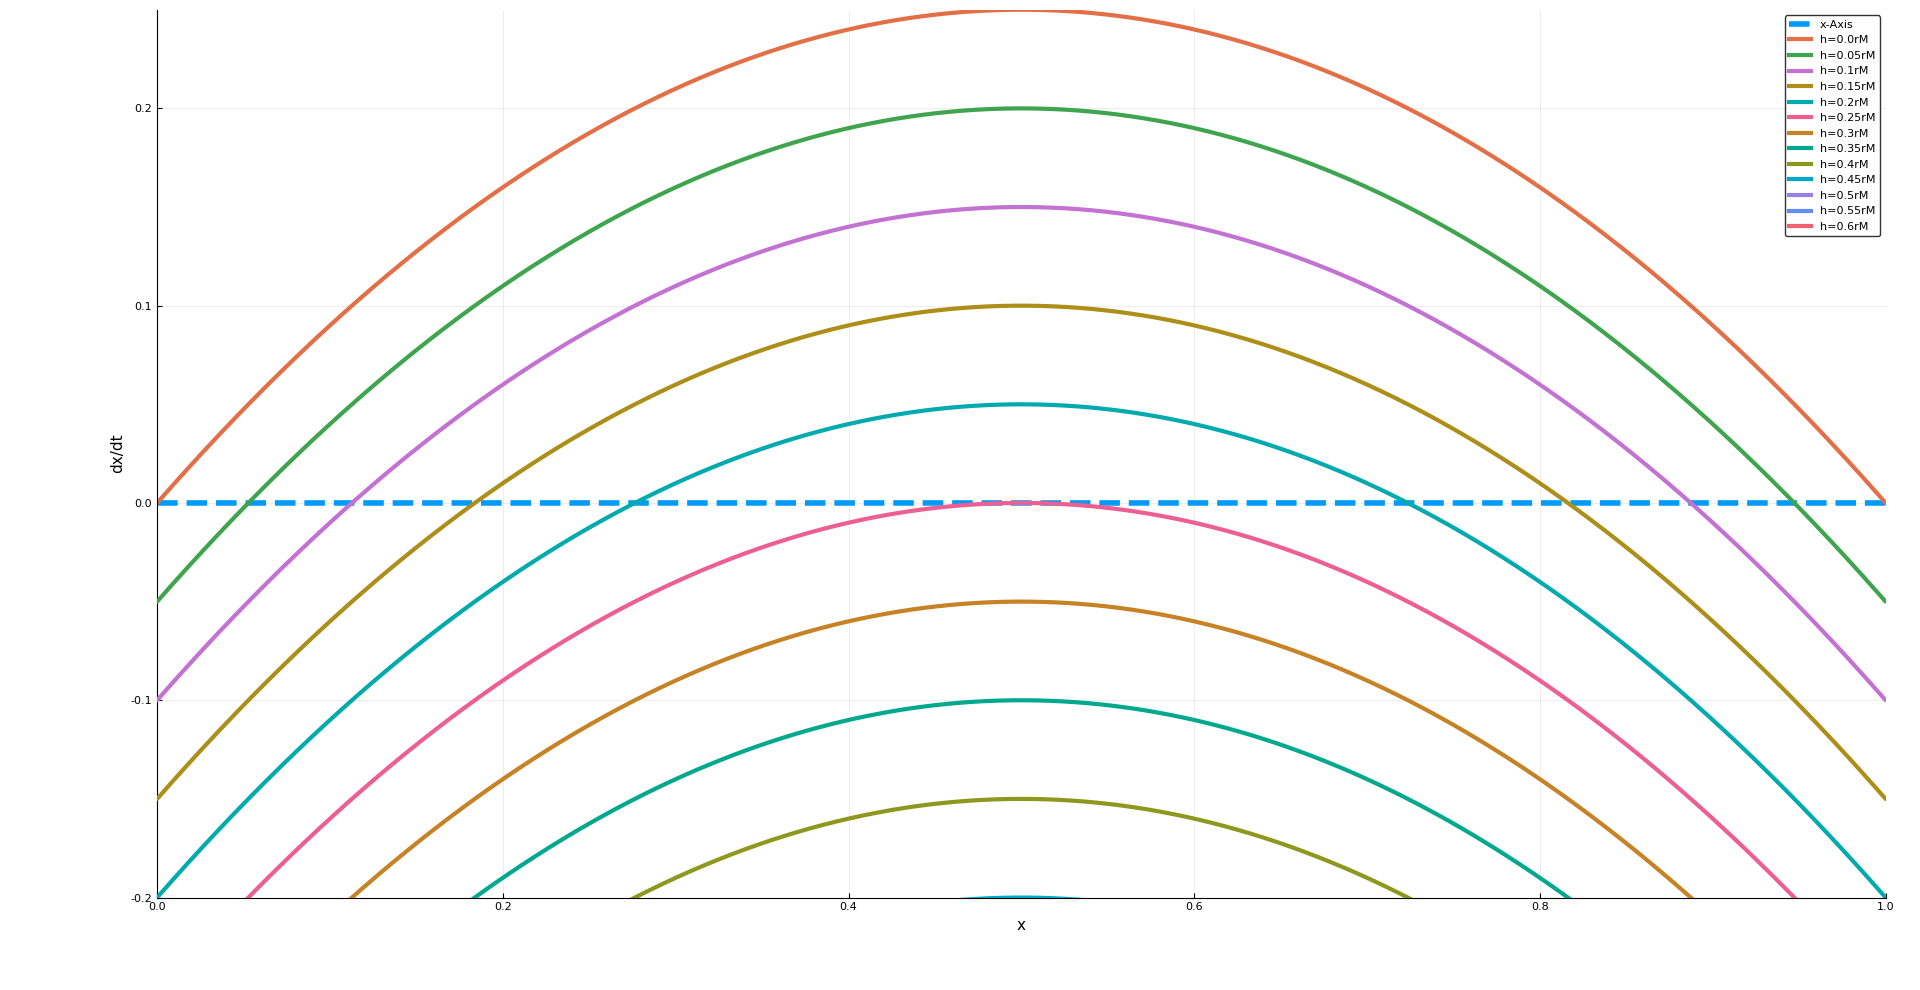
\includegraphics[width=0.8\textwidth]{CriticalPoints.png}
	\caption{Figure representing $\dev{x}{t}$ with different harvesting rates.}
	\label{fig: CriticalPoints}
\end{figure}
\begin{figure}
		\centering
		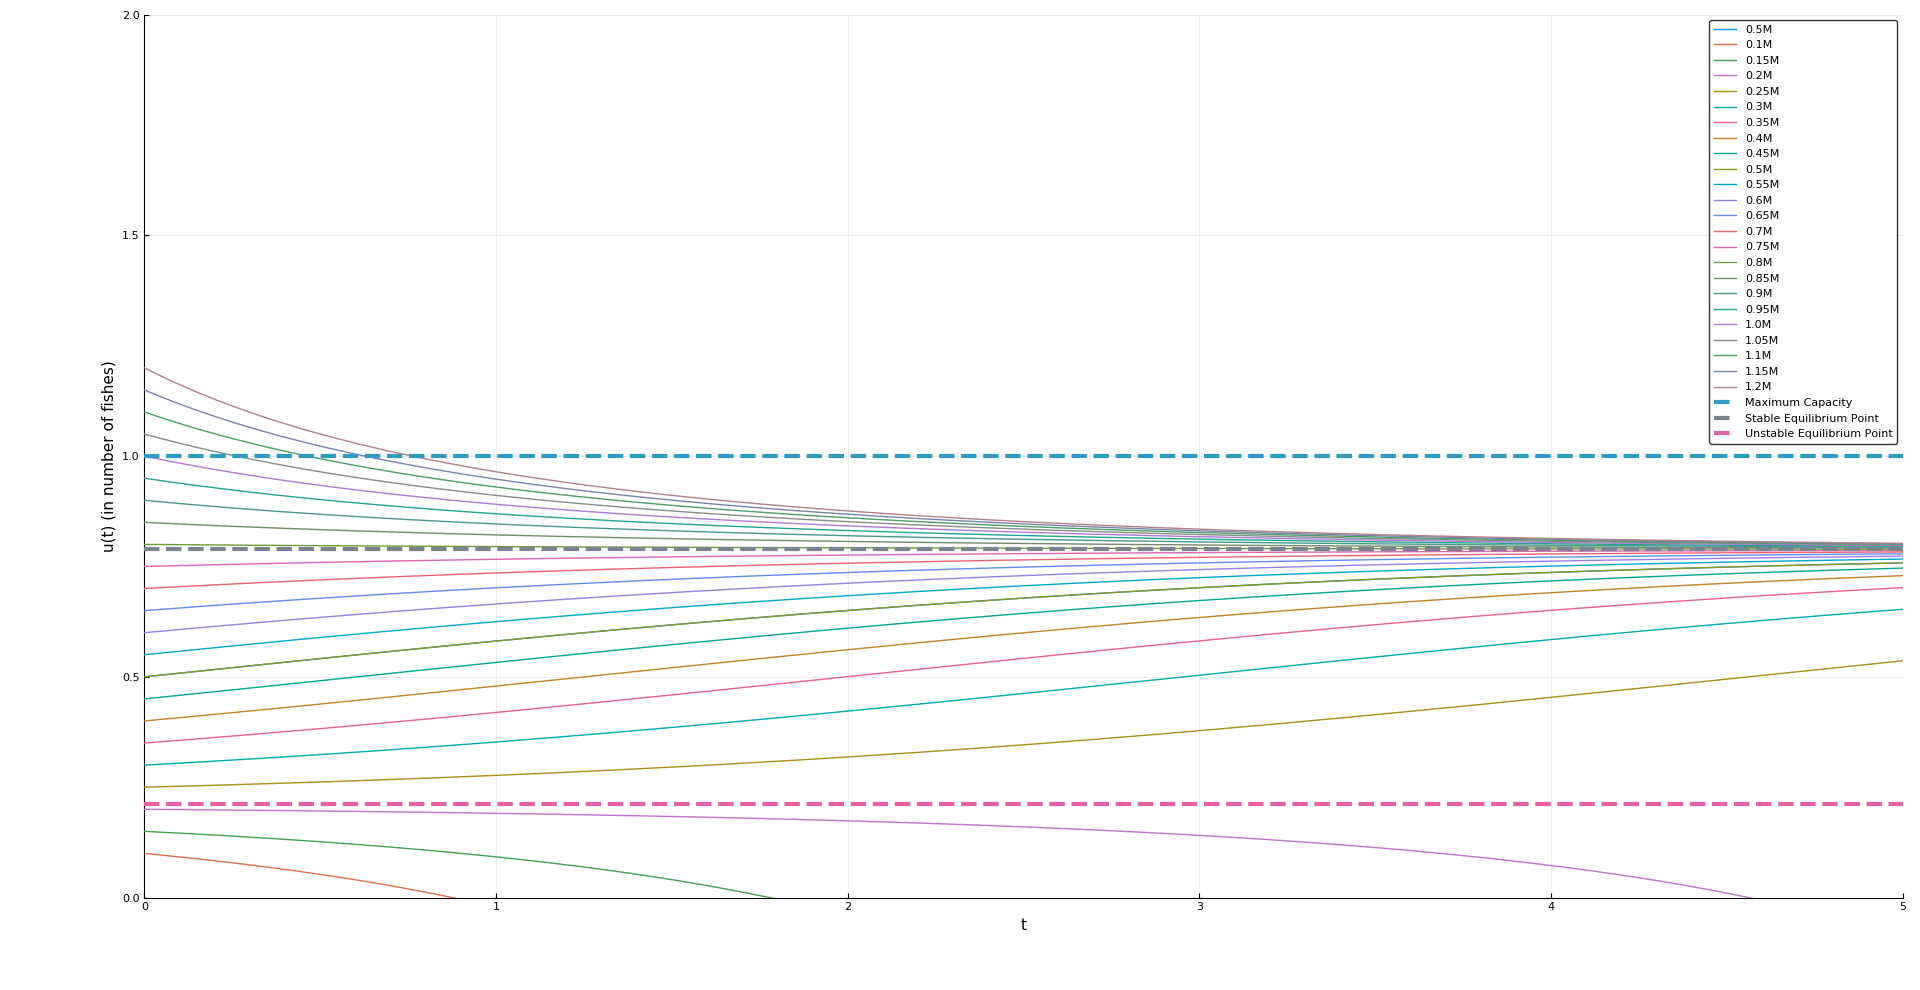
\includegraphics[width=0.8\textwidth]{SustainableConstant.png}
		\caption{Constant harvest rate $u<\frac{rM}{4}$.}
		\label{fig: SustainableConstantHarvest}
\end{figure}
\begin{figure}
	\centering
	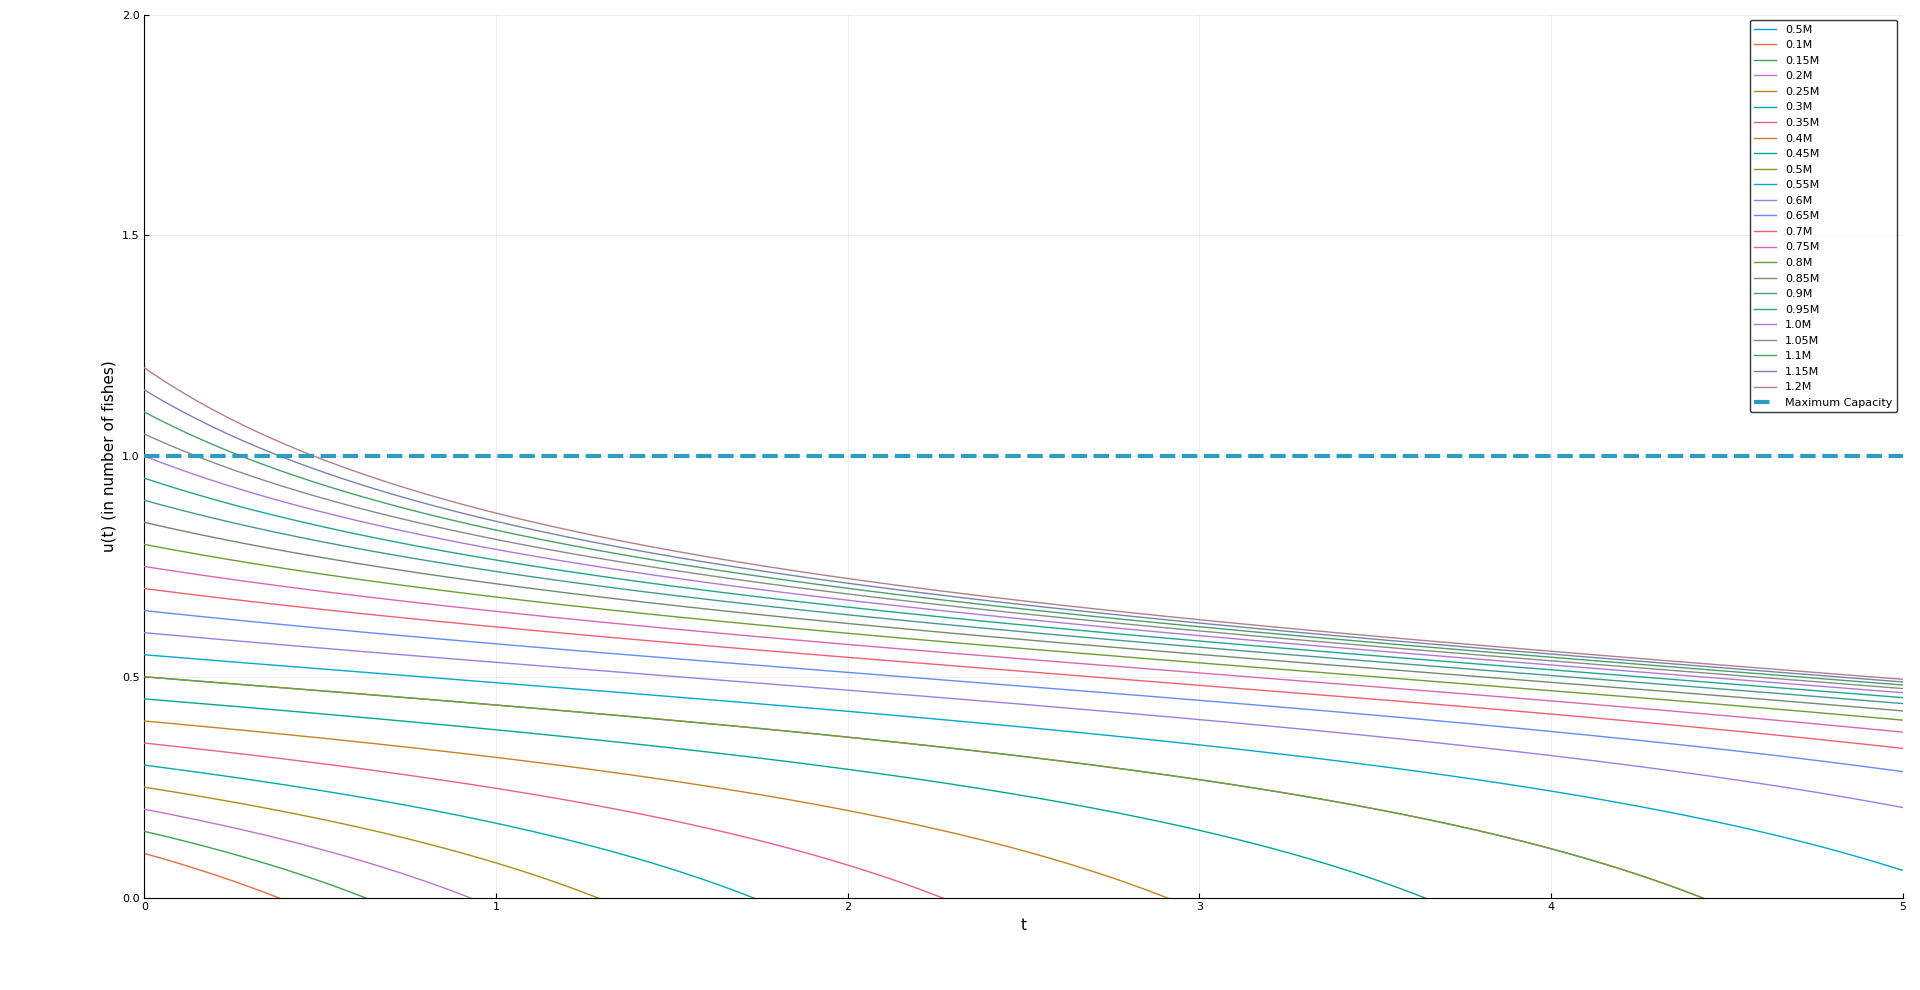
\includegraphics[width=0.8\textwidth]{OverExploitConstant.png}
	\caption{Constant harvest rate $u>\frac{rM}{4}$.}
	\label{fig: OverExploitConstantHarvest}
\end{figure}

\begin{figure}
	\centering
	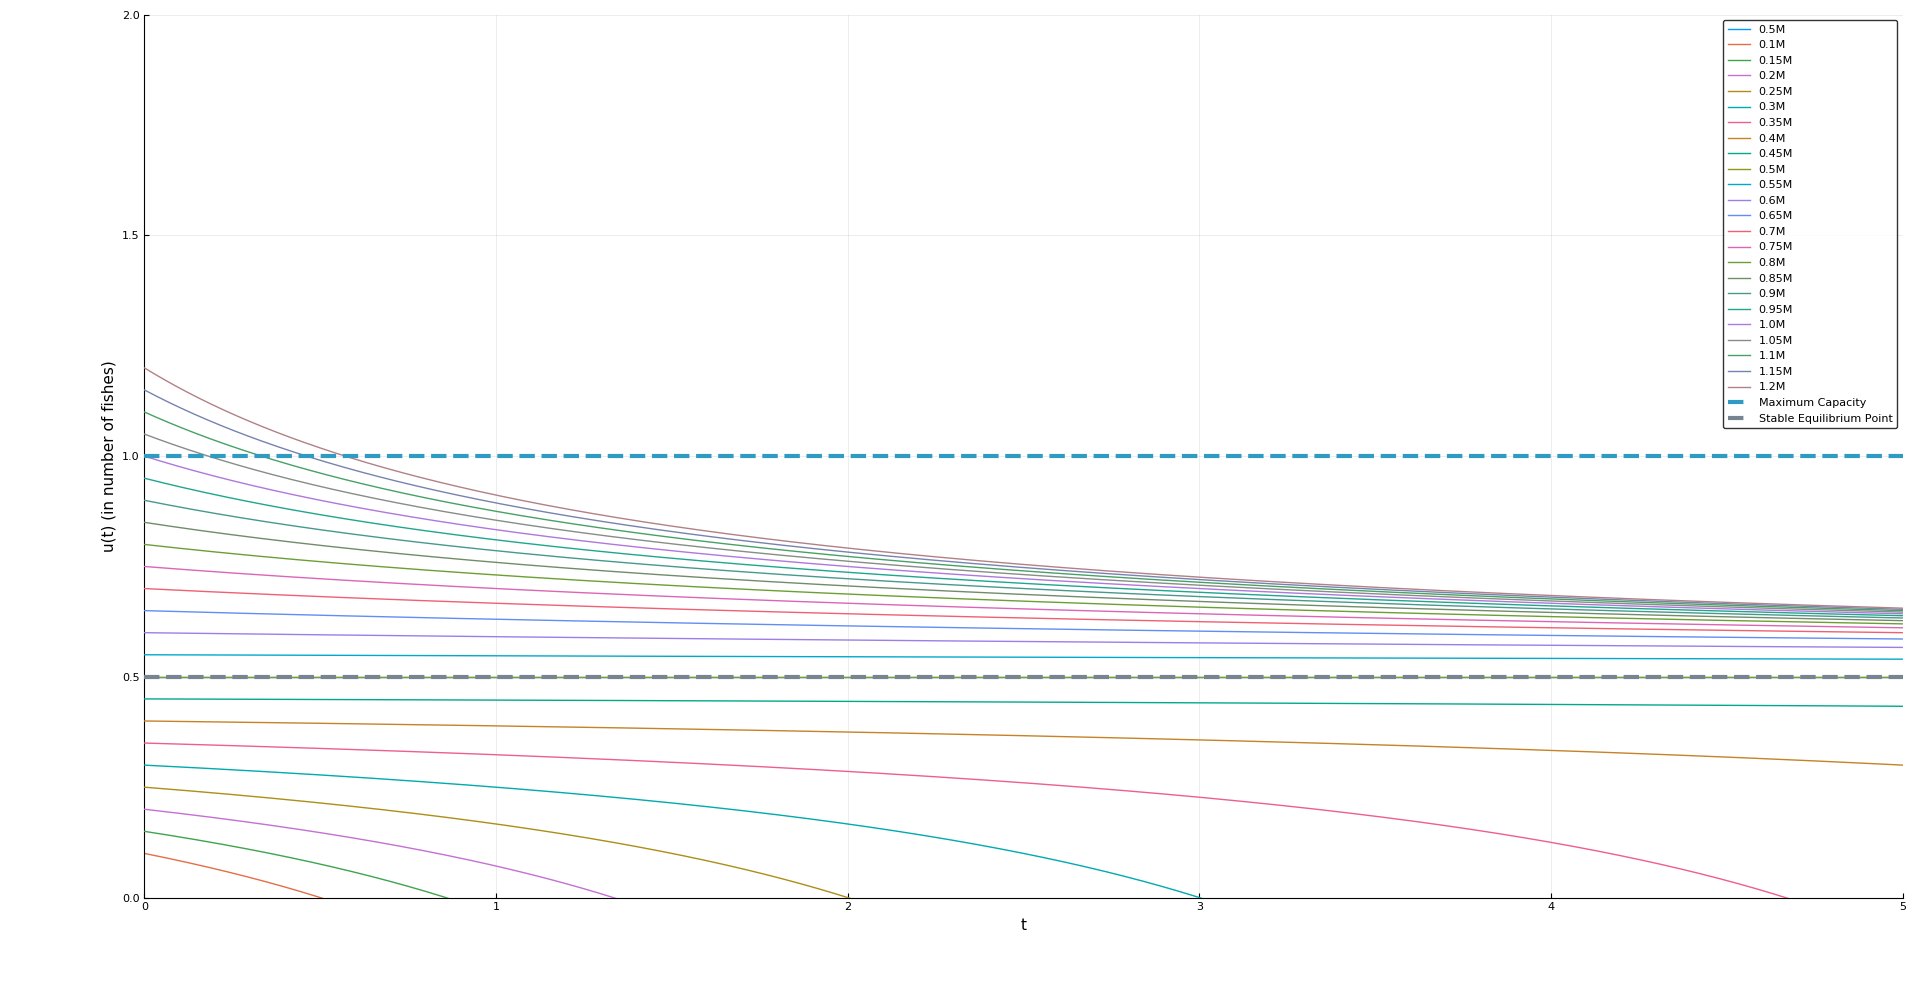
\includegraphics[width=0.8\textwidth]{CriticalExploitConstant.png}
	\caption{Constant harvest rate $u=\frac{rM}{4}$.}
	\label{fig: CriticalExploitConstantHarvest}
\end{figure}


	\section{Wiener Process and noise.} 
		\graphicspath{{Model/WienerProcess/}}
		\begin{equation}
\dev{x}{t}=rx\left(1-\frac{x}{M}\right)-u \label{eq: ConstantHarvest}
\end{equation}
We introduce the following variable in order to simply calculations,
\begin{equation}
\beta=\frac{uM}{r}
\end{equation}
Solving the differential equation,
\begin{align*}
	\frac{\diff{x}}{rx\left(1-\frac{x}{M}\right)-u}&=\diff{t} \\
	\int_{x_0}^{x}\frac{\diff{\chi}}{r\chi\left(1-\frac{\chi}{M}\right)-u}&=\int_{0}^{t}\diff{\tau} \\
	\frac{M}{r}\int_{x_0}^{x}\frac{\diff{\chi}}{\chi\left(M-\chi\right)-\frac{Mu}{r}}&=t \\
	-\frac{M}{r}\int_{x_0}^{x}\frac{\diff{\chi}}{\chi^2-M\chi+\beta}&=t \nonumber
	\end{align*}
Finally, we model the above integral as one 
\begin{align}
	-\frac{M}{r}\int_{x_0}^{x}\frac{\diff{\chi}}{\left(\chi-\frac{M}{2}\right)^2-\frac{M^2}{4}+\beta}&=t
\end{align}
Consider $\alpha$ as follows,
\begin{equation}
	\alpha = \beta - \frac{M^2}{4} = rM\left(u-\frac{rM}{4}\right)
\end{equation}
We see that the sign of $\alpha$ determines the nature of the solutions. Then, if $u>rM/4$ implies $\alpha>0$,
\begin{align*}
\int_{x_0}^{x}\frac{\diff{\chi}}{\left(\chi-\frac{M}{2}\right)^2+\alpha}&=-\frac{r}{M}t \\
\frac{1}{\sqrt{\beta-\frac{M^2}{4}}}\left(\arctan\left(\frac{x-M/2}{\sqrt{\beta-M^2/4}}\right)-\arctan\left(\frac{x_0-M/2}{\sqrt{\beta-M^2/4}}\right)\right)&=-\frac{r}{M}t \\
\end{align*}
Therefore, for $\alpha > 0$ the population behaves as follows, 
\begin{align}
	x(t)=\frac{M}{2}+\sqrt{\beta-\frac{M^2}{4}} \tan \left(\arctan\left(\frac{x_0-M/2}{\sqrt{\beta-M^2/4}}\right)-\frac{r\sqrt{\beta-M^2/4}}{M}t\right) \label{eq: ConstantHarvest OverExploit}
\end{align}

Equation \ref{eq: ConstantHarvest OverExploit} show us that for some $t^*$, $x(t^*)=0$,independently of the initial condition $x_0$, since the argument inside the $\tan$ is monotone decreasing in $t$. 

If $u<rM/4$ implies $-\alpha>0$,
\begin{align*}
	\int_{x_0}^{x}\frac{\diff{\chi}}{\left(\chi-\frac{M}{2}\right)^2-(-\alpha)} &=-\frac{r}{M}t
\end{align*}
Considering the zeros of the denominator, $\lambda$ and $\overleftarrow{\lambda}$, 
\begin{equation}
	\begin{array}{cc}
	\lambda&=\frac{M}{2}+\sqrt{\frac{M^2}{4}-\beta} \\
	\overline{\lambda}&=\frac{M}{2}-\sqrt{\frac{M^2}{4}-\beta} \\
	\end{array}
\end{equation}
We can rewrite our expression as follows, 
\begin{align*}
\int_{x_0}^{x} \left(\frac{1}{\chi - \lambda}-\frac{1}{\chi - \overline{\lambda}}\right)\diff{\chi} &=-\frac{2r\sqrt{M^2/4-\beta}}{M}t \\
	\ln\abs{\frac{x - \lambda}{x - \overline{\lambda}}}&=\ln\abs{\frac{x_0- \lambda}{x_0 - \overline{\lambda}}}-\frac{2r\sqrt{M^2/4-\beta}}{M}t
\end{align*}
For simplifying calculations, we write, $\gamma=\frac{2r\sqrt{M^2/4-\beta}}{M}$. And we obtain as result,
\begin{align}
\frac{x - \lambda}{x - \overline{\lambda}} &=\frac{x_0- \lambda}{x_0- \overline{\lambda}}\mathrm e^{-\gamma t} \\
x-\lambda &=\left(x-\overline{\lambda}\right)\left(\frac{x_0- \lambda}{x_0- \overline{\lambda}}\right)\mathrm e^{-\gamma t}
\end{align}

For the sake of simplicity, consider $\xi=\frac{x_0-\lambda}{x_0-\overline{\lambda}}\mathrm{e}^{-\gamma t}$. Therefore,
\begin{align*}
	x\left(1-\xi\right)&=\lambda-\overline{\lambda}\xi\\
	x&=\frac{\lambda-\overline{\lambda}\xi}{1-\xi} \\	
	x&=\frac{\frac{M}{2}+\sqrt{\frac{M^2}{4}-\beta}-\left(\frac{M}{2}-\sqrt{\frac{M^2}{4}-\beta}\right)\xi}{1-\xi}\\
	x&=\frac{\frac{M}{2}+\sqrt{\frac{M^2}{4}-\beta}-\left(\frac{M}{2}-\sqrt{\frac{M^2}{4}-\beta}\right)\xi}{1-\xi}\\
	x&=\frac{\frac{M}{2}\left(1-\xi\right)+\sqrt{\frac{M^2}{4}-\beta}\left(1+\xi\right)}{1-\xi}\\
	x&=\frac{M}{2}+\sqrt{\frac{M^2}{4}-\beta}\frac{1+\xi}{1-\xi}
\end{align*}
Hence, for $-\alpha>0$, we have the following result,
\begin{align}
	x(t)&=\frac{M}{2}+\left(\sqrt{\frac{M^2}{4}-\beta}\right)\frac{\left(x_0-M/2\right)\left(1+\mathrm e^{-\gamma t}\right)-\sqrt{M^2/4-\beta}\left(1-\mathrm{e}^{-\gamma t}\right)}{\left(x_0-M/2\right)\left(1-\mathrm e^{-\gamma t}\right)+\sqrt{M^2/4-\beta}\left(1+\mathrm{e}^{-\gamma t}\right)} \label{eq: Time Expression for Harvest}
\end{align}

If $u=\frac{rM}{4}$, we solve equation \ref{eq: ConstantHarvest} as follows,
\begin{align}
-\frac{M}{r}\int_{x_0}^{x}\frac{d\chi}{\left(\chi-\frac{M}{2}\right)^2}&=t\\
\int_{x_0}^{x}\frac{d\chi}{\left(\chi-\frac{M}{2}\right)^2}&=-\frac{rt}{M}\\
\frac{1}{x-\frac{M}{2}}&=\frac{1}{x_0-\frac{M}{2}}-\frac{rt}{M}\\
\frac{1}{x-\frac{M}{2}}&=\frac{M-\left(x_0-\frac{M}{2}\right)rt}{M\left(x_0-\frac{M}{2}\right)} \\
x&=\frac{M}{2}+\frac{M\left(x_0-\frac{M}{2}\right)}{M-\left(x_0-\frac{M}{2}\right)rt} 
\end{align}

The results above stated can be explained directly from the equation \ref{eq: ConstantHarvest}, as we see in the graph \ref{fig: CriticalPoints},  $F(x,t)$ is a paraboloid, with its maximum at $F(x^*=M/2,t)=rM^2/4$.

When $u=0$, we have the regular logistic equation with critical points $x_{c_1}=0$ and $x_{c_2}=M$. With $x_{c_2}$ being an stable fixed point and $x_{c_1}$ an unstable fixed point. In general, these are the solutions to the equation $F(x,t)-u=0$,
\begin{equation}
x_{c_{2,1}}=\frac{M}{2}\pm \sqrt{\frac{M^2}{4}-u\frac{M}{r}}
\end{equation}

We observe that the critical points $x_c$, such that $\dev{x_c}{t}=F(x_c, t)-u=0$ are getting closer to each other, as $u$ is increasing; when $u=\frac{rM}{4}$ we only have one critical unstable point. That behaves as an attractor when $x_0\geq\frac{M}{2}$. But when $x_0<\frac{M}{2}$ the population strictly decreases. For $u> \frac{rM}{4}$, the population $x(t)$ has no real critical points and the derivative $\dev{x}{t}$ is always negative, implying, that we will lead always the population to extinction, extracting constantly at a rate greater than $\frac{rM}{4}$.

\begin{figure}[H]
	\centering
	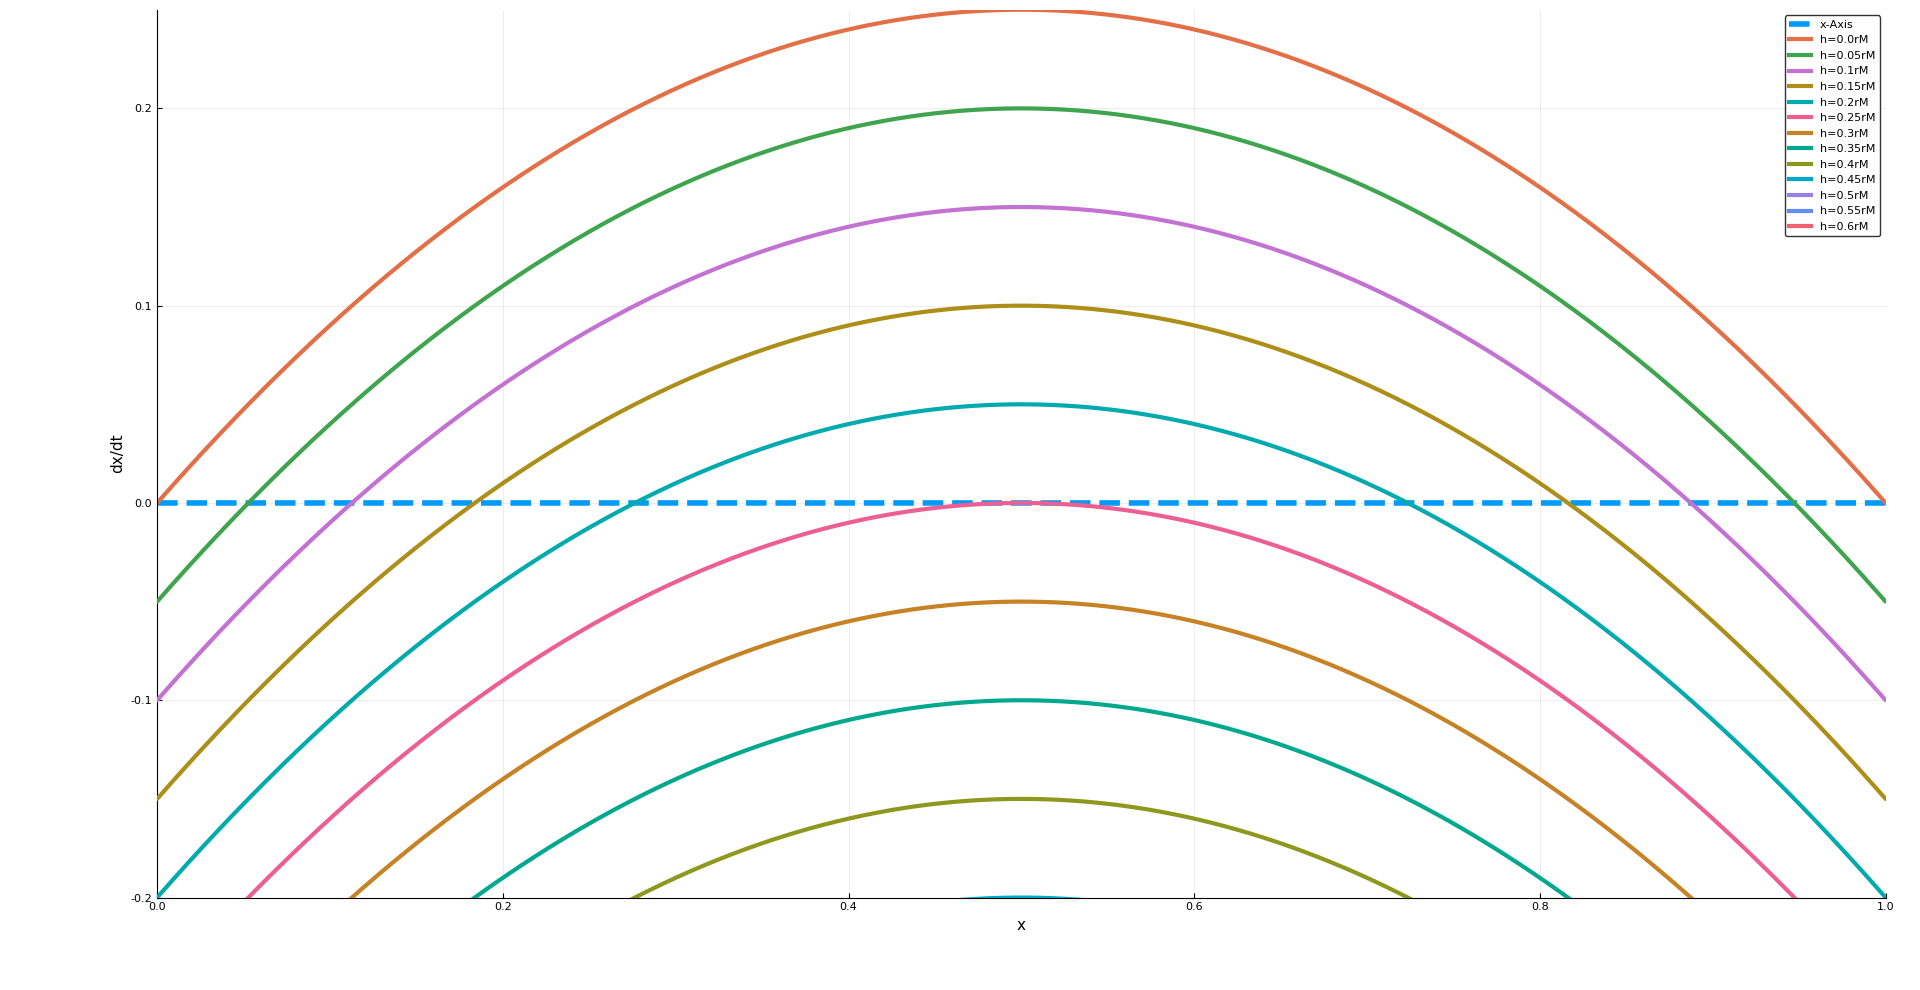
\includegraphics[width=0.8\textwidth]{CriticalPoints.png}
	\caption{Figure representing $\dev{x}{t}$ with different harvesting rates.}
	\label{fig: CriticalPoints}
\end{figure}
\begin{figure}
		\centering
		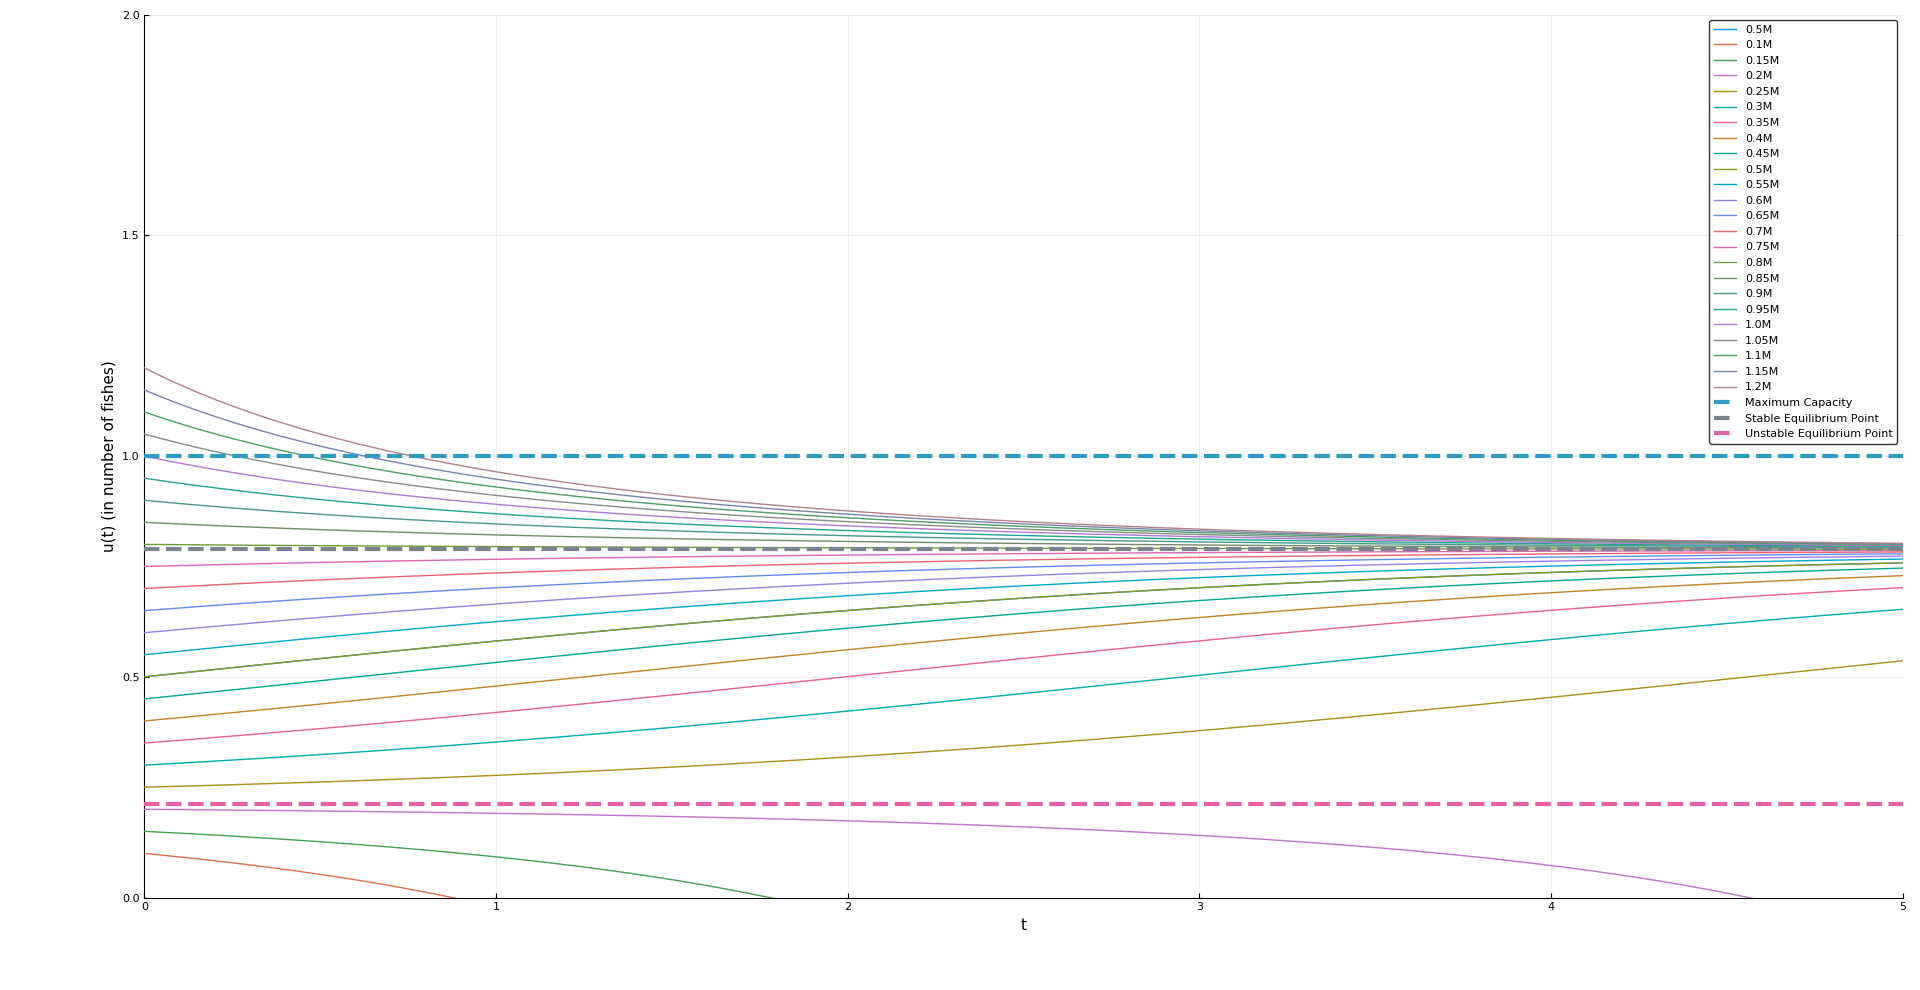
\includegraphics[width=0.8\textwidth]{SustainableConstant.png}
		\caption{Constant harvest rate $u<\frac{rM}{4}$.}
		\label{fig: SustainableConstantHarvest}
\end{figure}
\begin{figure}
	\centering
	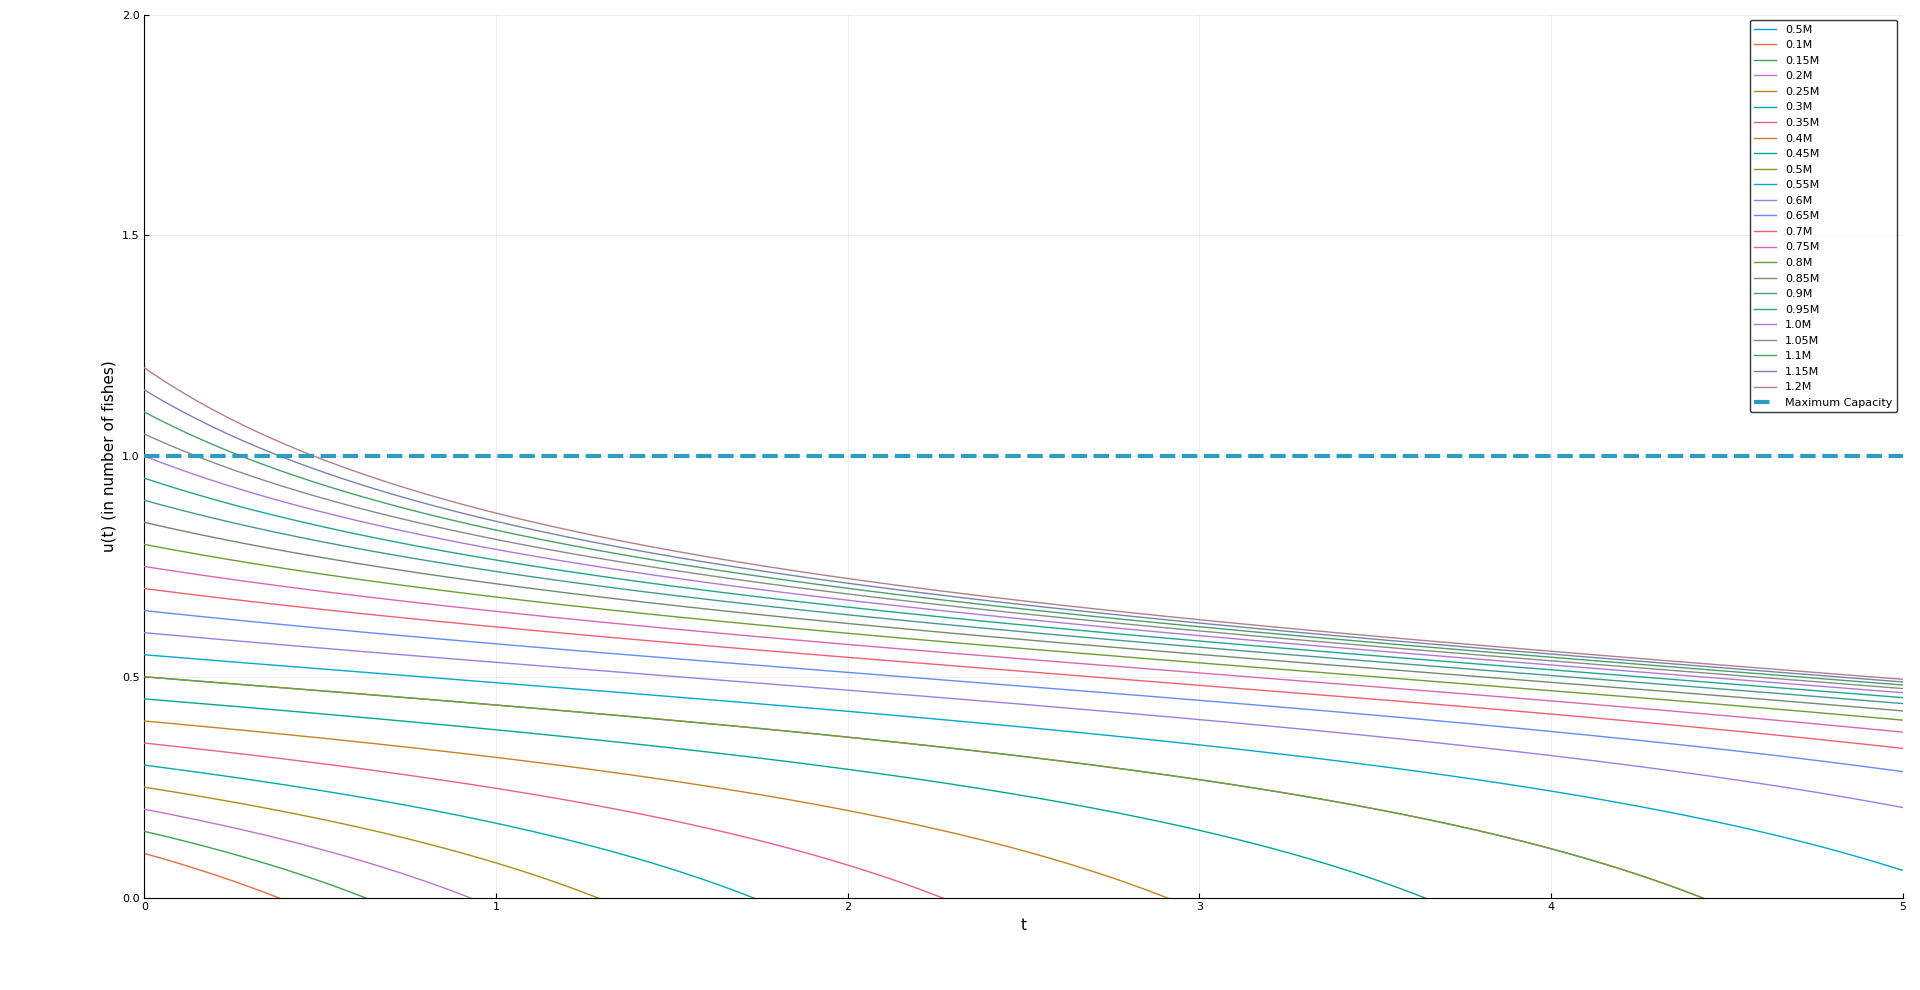
\includegraphics[width=0.8\textwidth]{OverExploitConstant.png}
	\caption{Constant harvest rate $u>\frac{rM}{4}$.}
	\label{fig: OverExploitConstantHarvest}
\end{figure}

\begin{figure}
	\centering
	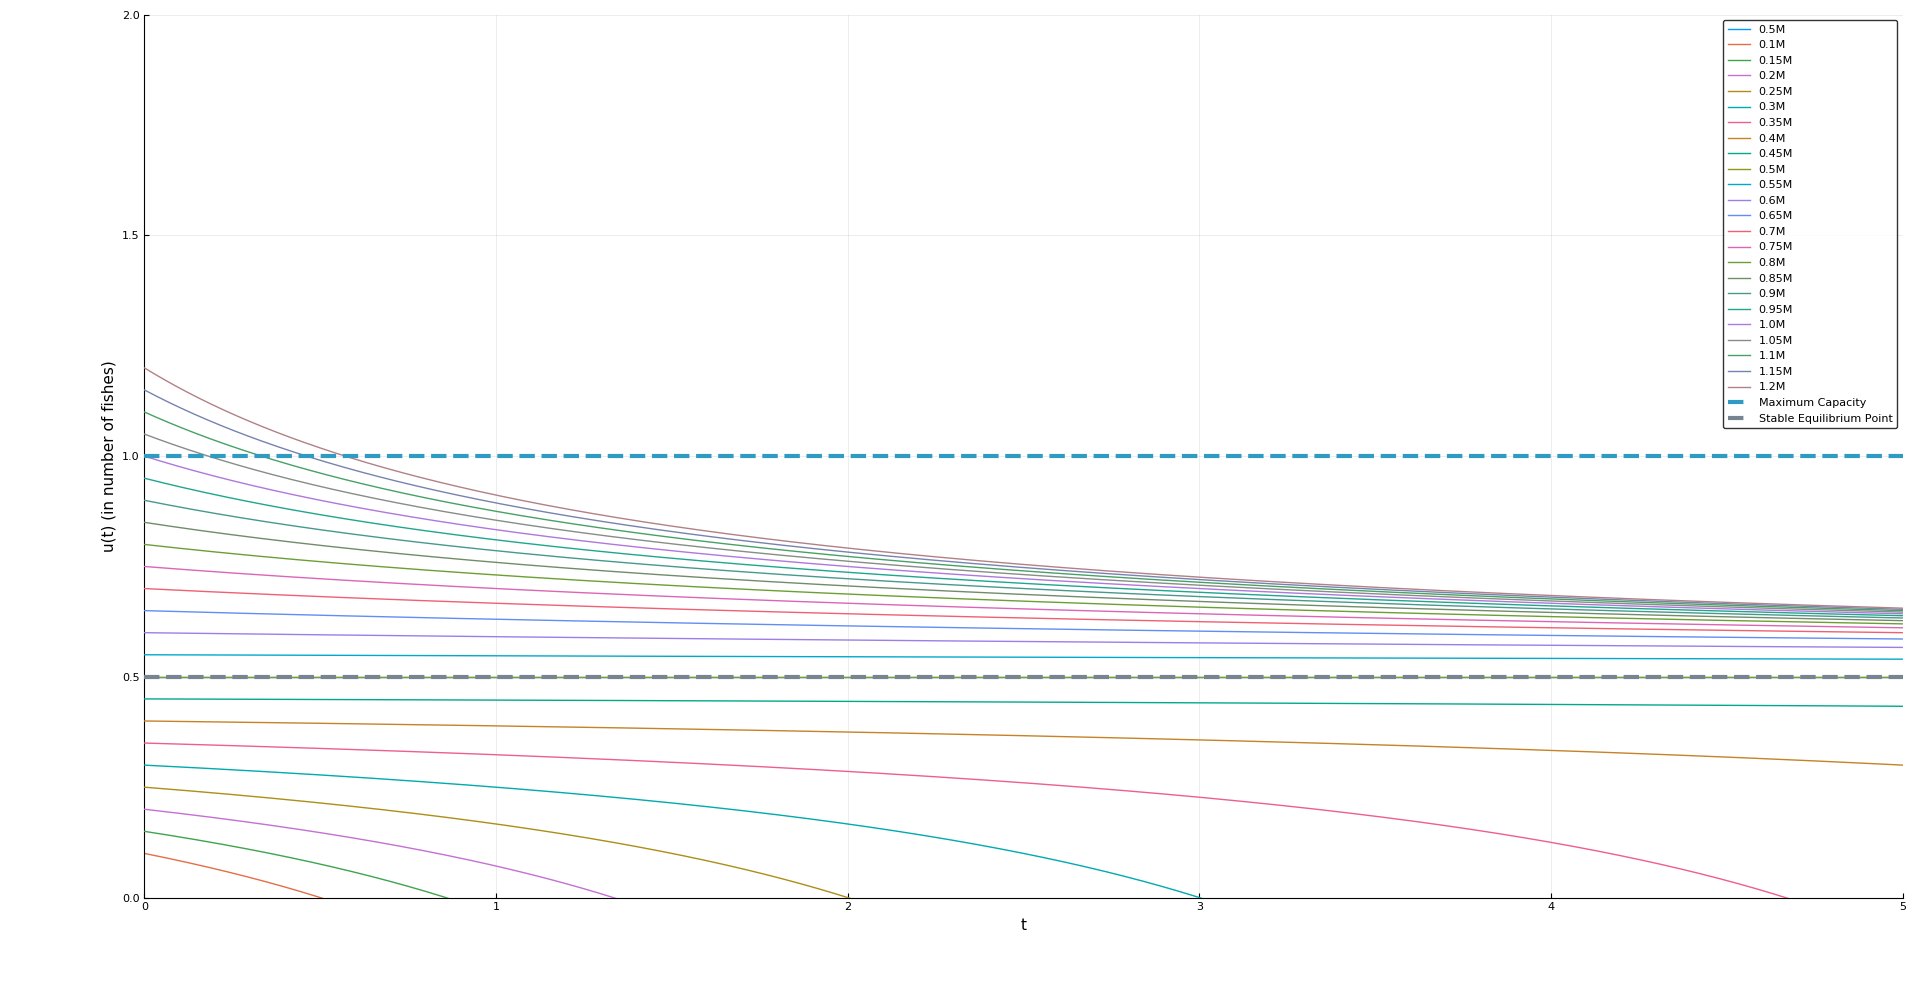
\includegraphics[width=0.8\textwidth]{CriticalExploitConstant.png}
	\caption{Constant harvest rate $u=\frac{rM}{4}$.}
	\label{fig: CriticalExploitConstantHarvest}
\end{figure}


\chapter{Fishing Strategies and Optimizing Population} \label{chap: Fishing Strategies}
	\begin{equation}
\dev{x}{t}=rx\left(1-\frac{x}{M}\right)-u \label{eq: ConstantHarvest}
\end{equation}
We introduce the following variable in order to simply calculations,
\begin{equation}
\beta=\frac{uM}{r}
\end{equation}
Solving the differential equation,
\begin{align*}
	\frac{\diff{x}}{rx\left(1-\frac{x}{M}\right)-u}&=\diff{t} \\
	\int_{x_0}^{x}\frac{\diff{\chi}}{r\chi\left(1-\frac{\chi}{M}\right)-u}&=\int_{0}^{t}\diff{\tau} \\
	\frac{M}{r}\int_{x_0}^{x}\frac{\diff{\chi}}{\chi\left(M-\chi\right)-\frac{Mu}{r}}&=t \\
	-\frac{M}{r}\int_{x_0}^{x}\frac{\diff{\chi}}{\chi^2-M\chi+\beta}&=t \nonumber
	\end{align*}
Finally, we model the above integral as one 
\begin{align}
	-\frac{M}{r}\int_{x_0}^{x}\frac{\diff{\chi}}{\left(\chi-\frac{M}{2}\right)^2-\frac{M^2}{4}+\beta}&=t
\end{align}
Consider $\alpha$ as follows,
\begin{equation}
	\alpha = \beta - \frac{M^2}{4} = rM\left(u-\frac{rM}{4}\right)
\end{equation}
We see that the sign of $\alpha$ determines the nature of the solutions. Then, if $u>rM/4$ implies $\alpha>0$,
\begin{align*}
\int_{x_0}^{x}\frac{\diff{\chi}}{\left(\chi-\frac{M}{2}\right)^2+\alpha}&=-\frac{r}{M}t \\
\frac{1}{\sqrt{\beta-\frac{M^2}{4}}}\left(\arctan\left(\frac{x-M/2}{\sqrt{\beta-M^2/4}}\right)-\arctan\left(\frac{x_0-M/2}{\sqrt{\beta-M^2/4}}\right)\right)&=-\frac{r}{M}t \\
\end{align*}
Therefore, for $\alpha > 0$ the population behaves as follows, 
\begin{align}
	x(t)=\frac{M}{2}+\sqrt{\beta-\frac{M^2}{4}} \tan \left(\arctan\left(\frac{x_0-M/2}{\sqrt{\beta-M^2/4}}\right)-\frac{r\sqrt{\beta-M^2/4}}{M}t\right) \label{eq: ConstantHarvest OverExploit}
\end{align}

Equation \ref{eq: ConstantHarvest OverExploit} show us that for some $t^*$, $x(t^*)=0$,independently of the initial condition $x_0$, since the argument inside the $\tan$ is monotone decreasing in $t$. 

If $u<rM/4$ implies $-\alpha>0$,
\begin{align*}
	\int_{x_0}^{x}\frac{\diff{\chi}}{\left(\chi-\frac{M}{2}\right)^2-(-\alpha)} &=-\frac{r}{M}t
\end{align*}
Considering the zeros of the denominator, $\lambda$ and $\overleftarrow{\lambda}$, 
\begin{equation}
	\begin{array}{cc}
	\lambda&=\frac{M}{2}+\sqrt{\frac{M^2}{4}-\beta} \\
	\overline{\lambda}&=\frac{M}{2}-\sqrt{\frac{M^2}{4}-\beta} \\
	\end{array}
\end{equation}
We can rewrite our expression as follows, 
\begin{align*}
\int_{x_0}^{x} \left(\frac{1}{\chi - \lambda}-\frac{1}{\chi - \overline{\lambda}}\right)\diff{\chi} &=-\frac{2r\sqrt{M^2/4-\beta}}{M}t \\
	\ln\abs{\frac{x - \lambda}{x - \overline{\lambda}}}&=\ln\abs{\frac{x_0- \lambda}{x_0 - \overline{\lambda}}}-\frac{2r\sqrt{M^2/4-\beta}}{M}t
\end{align*}
For simplifying calculations, we write, $\gamma=\frac{2r\sqrt{M^2/4-\beta}}{M}$. And we obtain as result,
\begin{align}
\frac{x - \lambda}{x - \overline{\lambda}} &=\frac{x_0- \lambda}{x_0- \overline{\lambda}}\mathrm e^{-\gamma t} \\
x-\lambda &=\left(x-\overline{\lambda}\right)\left(\frac{x_0- \lambda}{x_0- \overline{\lambda}}\right)\mathrm e^{-\gamma t}
\end{align}

For the sake of simplicity, consider $\xi=\frac{x_0-\lambda}{x_0-\overline{\lambda}}\mathrm{e}^{-\gamma t}$. Therefore,
\begin{align*}
	x\left(1-\xi\right)&=\lambda-\overline{\lambda}\xi\\
	x&=\frac{\lambda-\overline{\lambda}\xi}{1-\xi} \\	
	x&=\frac{\frac{M}{2}+\sqrt{\frac{M^2}{4}-\beta}-\left(\frac{M}{2}-\sqrt{\frac{M^2}{4}-\beta}\right)\xi}{1-\xi}\\
	x&=\frac{\frac{M}{2}+\sqrt{\frac{M^2}{4}-\beta}-\left(\frac{M}{2}-\sqrt{\frac{M^2}{4}-\beta}\right)\xi}{1-\xi}\\
	x&=\frac{\frac{M}{2}\left(1-\xi\right)+\sqrt{\frac{M^2}{4}-\beta}\left(1+\xi\right)}{1-\xi}\\
	x&=\frac{M}{2}+\sqrt{\frac{M^2}{4}-\beta}\frac{1+\xi}{1-\xi}
\end{align*}
Hence, for $-\alpha>0$, we have the following result,
\begin{align}
	x(t)&=\frac{M}{2}+\left(\sqrt{\frac{M^2}{4}-\beta}\right)\frac{\left(x_0-M/2\right)\left(1+\mathrm e^{-\gamma t}\right)-\sqrt{M^2/4-\beta}\left(1-\mathrm{e}^{-\gamma t}\right)}{\left(x_0-M/2\right)\left(1-\mathrm e^{-\gamma t}\right)+\sqrt{M^2/4-\beta}\left(1+\mathrm{e}^{-\gamma t}\right)} \label{eq: Time Expression for Harvest}
\end{align}

If $u=\frac{rM}{4}$, we solve equation \ref{eq: ConstantHarvest} as follows,
\begin{align}
-\frac{M}{r}\int_{x_0}^{x}\frac{d\chi}{\left(\chi-\frac{M}{2}\right)^2}&=t\\
\int_{x_0}^{x}\frac{d\chi}{\left(\chi-\frac{M}{2}\right)^2}&=-\frac{rt}{M}\\
\frac{1}{x-\frac{M}{2}}&=\frac{1}{x_0-\frac{M}{2}}-\frac{rt}{M}\\
\frac{1}{x-\frac{M}{2}}&=\frac{M-\left(x_0-\frac{M}{2}\right)rt}{M\left(x_0-\frac{M}{2}\right)} \\
x&=\frac{M}{2}+\frac{M\left(x_0-\frac{M}{2}\right)}{M-\left(x_0-\frac{M}{2}\right)rt} 
\end{align}

The results above stated can be explained directly from the equation \ref{eq: ConstantHarvest}, as we see in the graph \ref{fig: CriticalPoints},  $F(x,t)$ is a paraboloid, with its maximum at $F(x^*=M/2,t)=rM^2/4$.

When $u=0$, we have the regular logistic equation with critical points $x_{c_1}=0$ and $x_{c_2}=M$. With $x_{c_2}$ being an stable fixed point and $x_{c_1}$ an unstable fixed point. In general, these are the solutions to the equation $F(x,t)-u=0$,
\begin{equation}
x_{c_{2,1}}=\frac{M}{2}\pm \sqrt{\frac{M^2}{4}-u\frac{M}{r}}
\end{equation}

We observe that the critical points $x_c$, such that $\dev{x_c}{t}=F(x_c, t)-u=0$ are getting closer to each other, as $u$ is increasing; when $u=\frac{rM}{4}$ we only have one critical unstable point. That behaves as an attractor when $x_0\geq\frac{M}{2}$. But when $x_0<\frac{M}{2}$ the population strictly decreases. For $u> \frac{rM}{4}$, the population $x(t)$ has no real critical points and the derivative $\dev{x}{t}$ is always negative, implying, that we will lead always the population to extinction, extracting constantly at a rate greater than $\frac{rM}{4}$.

\begin{figure}[H]
	\centering
	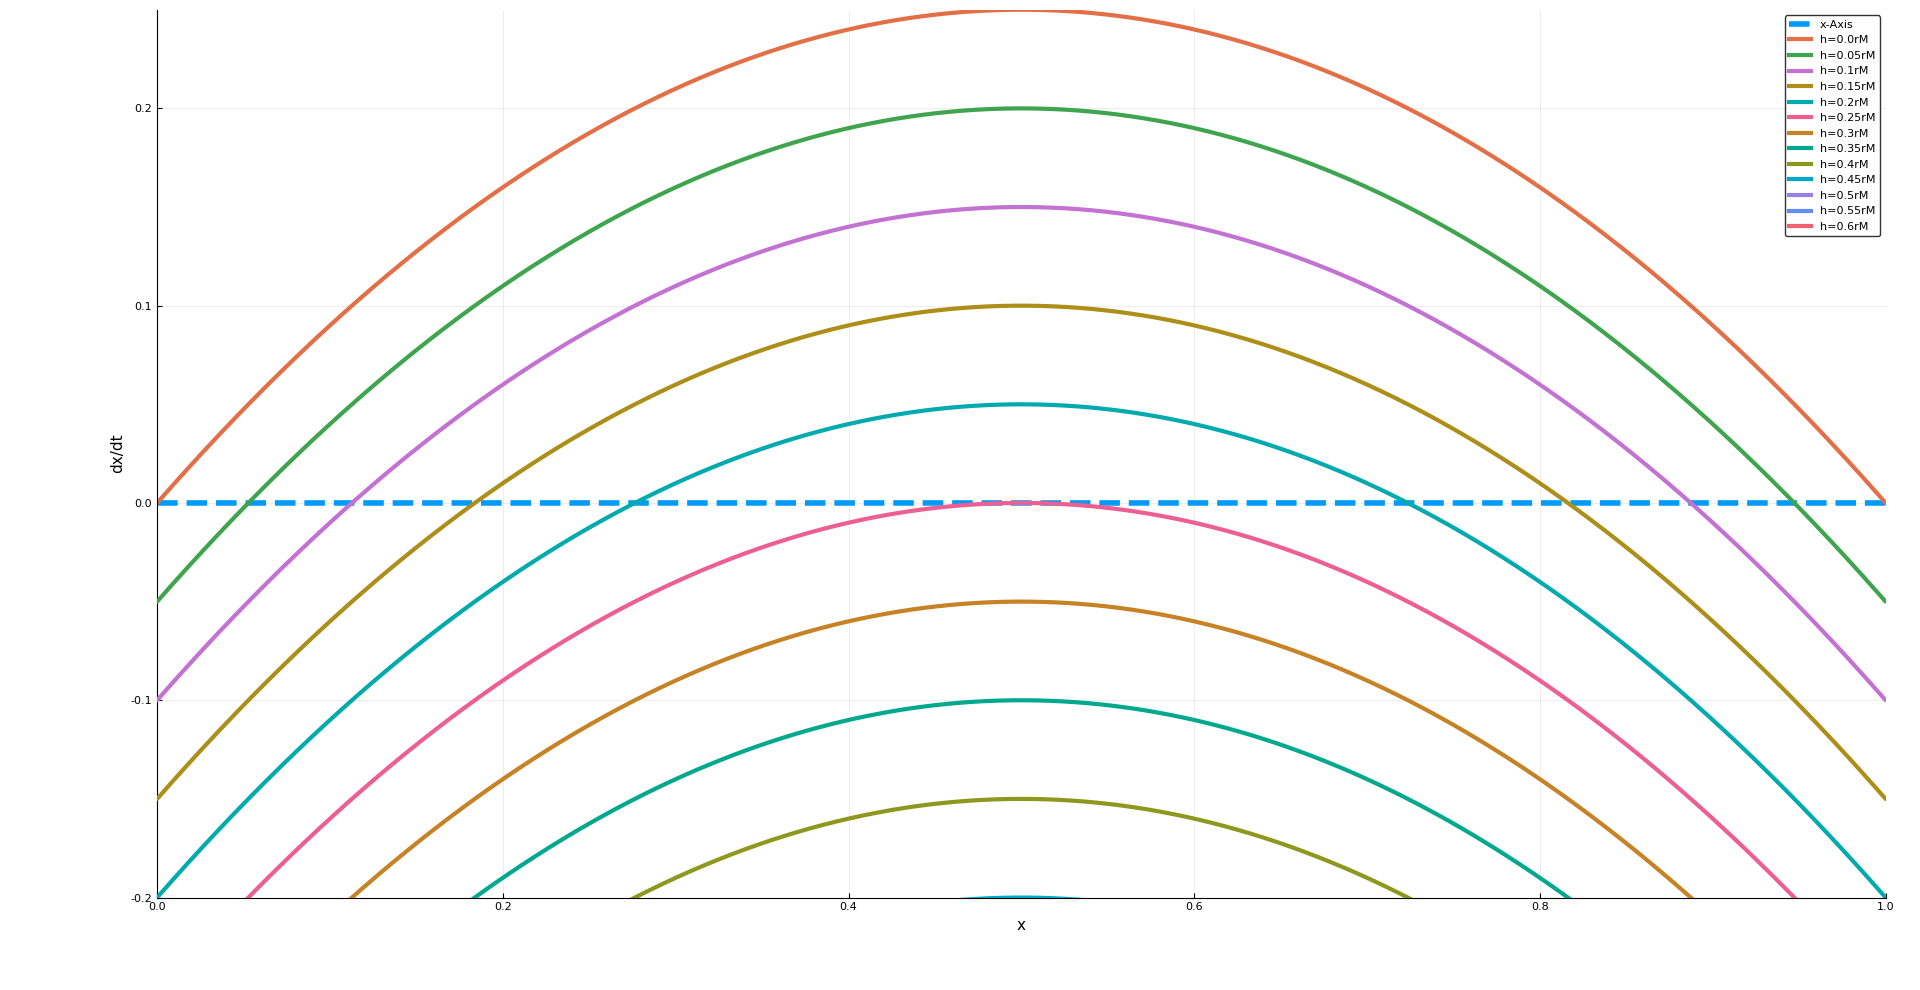
\includegraphics[width=0.8\textwidth]{CriticalPoints.png}
	\caption{Figure representing $\dev{x}{t}$ with different harvesting rates.}
	\label{fig: CriticalPoints}
\end{figure}
\begin{figure}
		\centering
		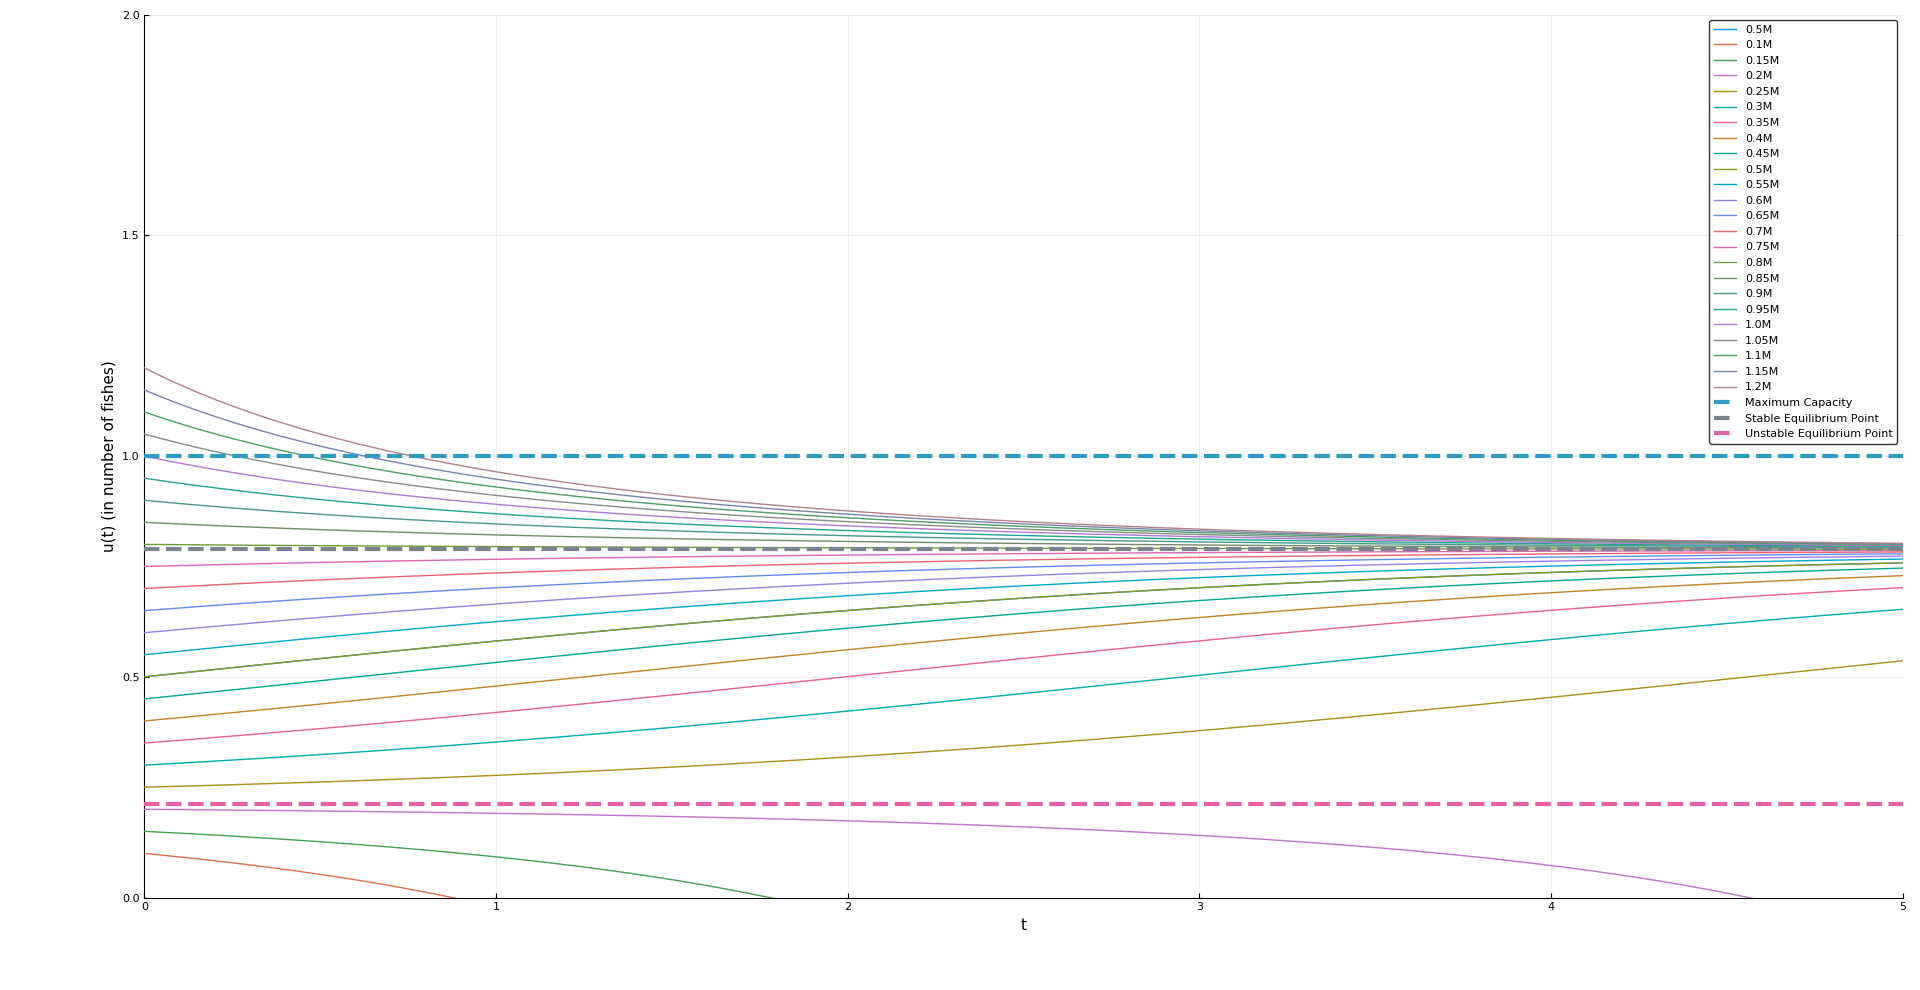
\includegraphics[width=0.8\textwidth]{SustainableConstant.png}
		\caption{Constant harvest rate $u<\frac{rM}{4}$.}
		\label{fig: SustainableConstantHarvest}
\end{figure}
\begin{figure}
	\centering
	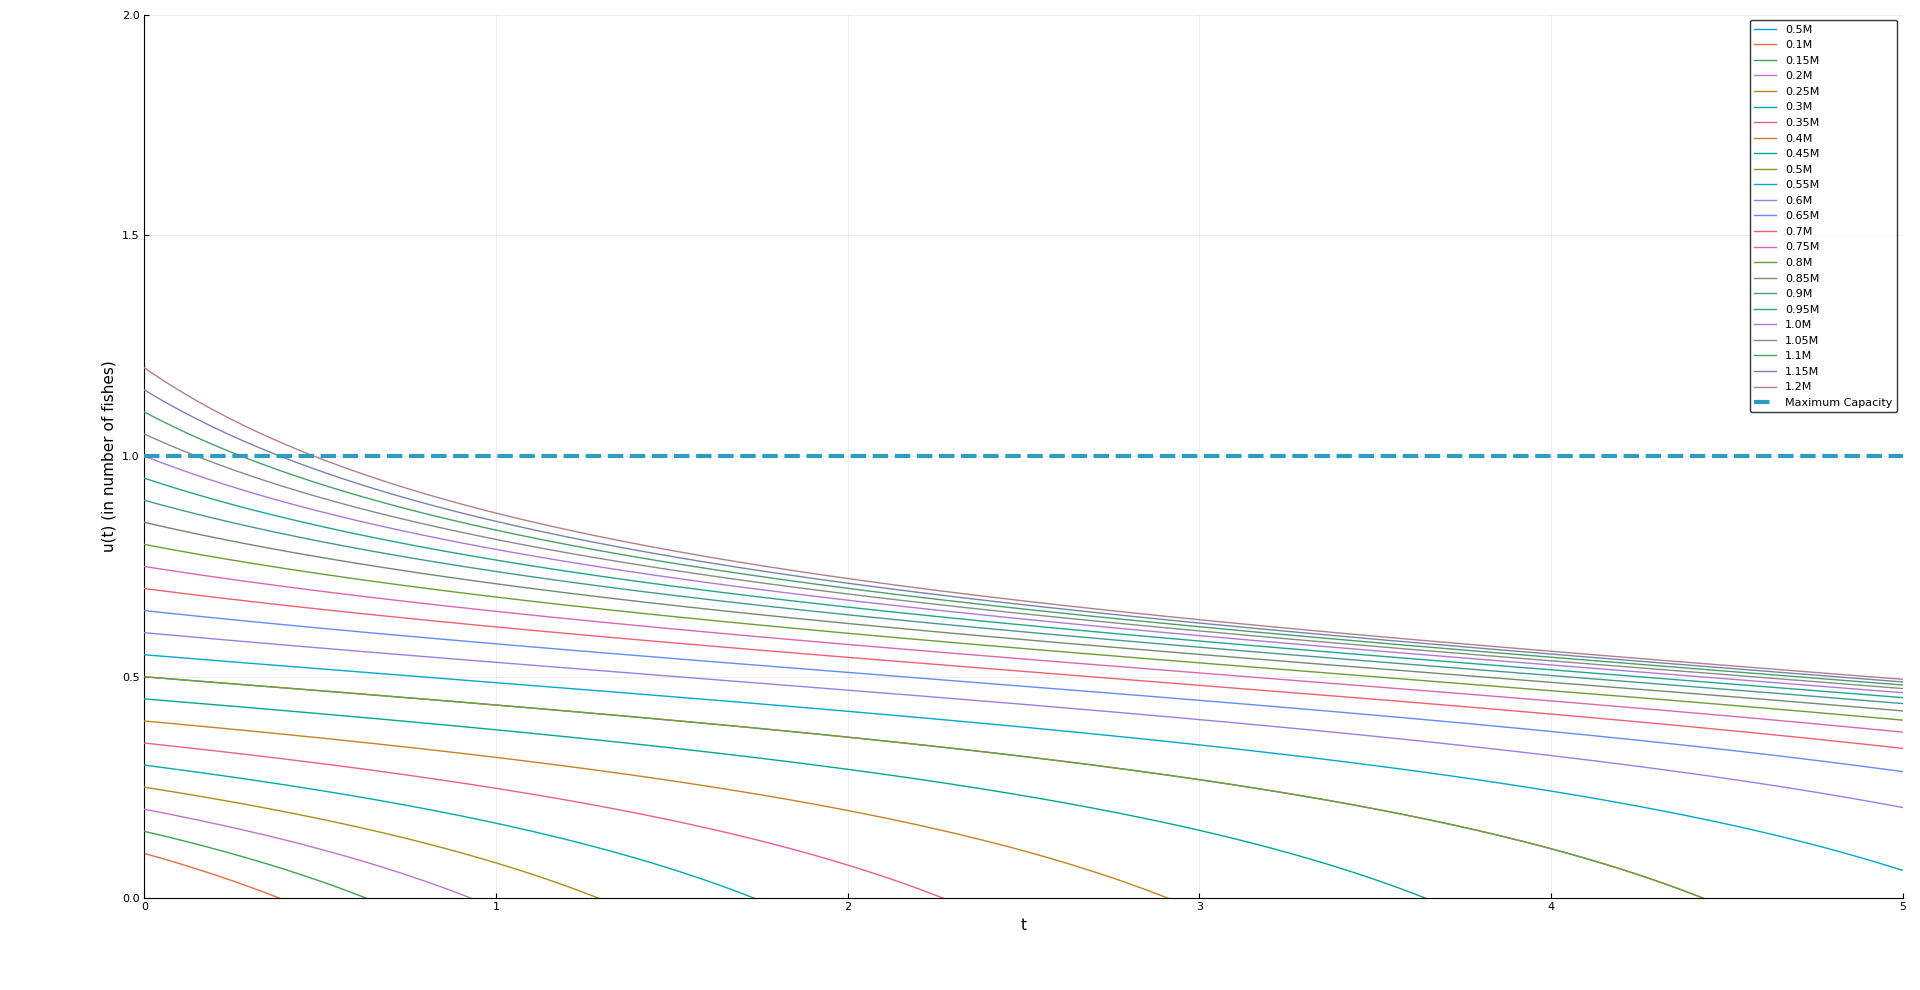
\includegraphics[width=0.8\textwidth]{OverExploitConstant.png}
	\caption{Constant harvest rate $u>\frac{rM}{4}$.}
	\label{fig: OverExploitConstantHarvest}
\end{figure}

\begin{figure}
	\centering
	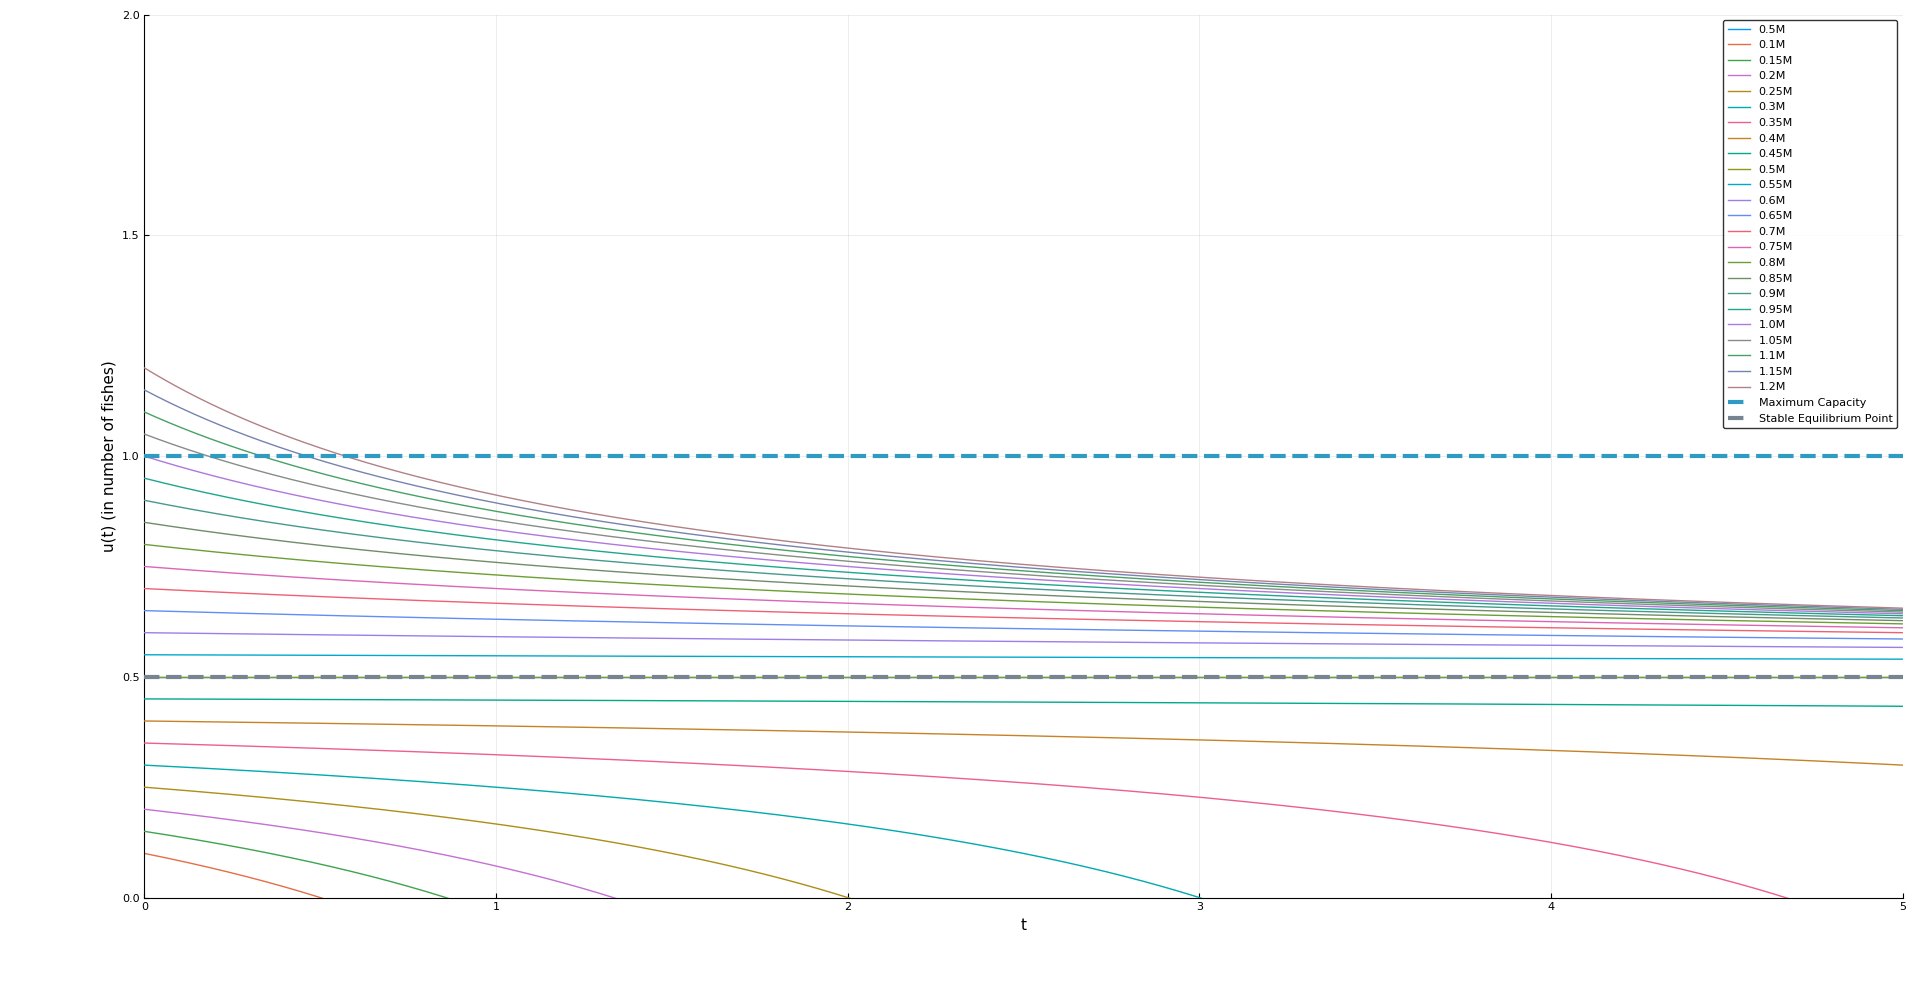
\includegraphics[width=0.8\textwidth]{CriticalExploitConstant.png}
	\caption{Constant harvest rate $u=\frac{rM}{4}$.}
	\label{fig: CriticalExploitConstantHarvest}
\end{figure}


	\section{Open Loop Strategies.}
	\graphicspath{{FishingStrategies/OpenLoop/}{FishingStrategies/OpenLoop/ConstantHarvest/}{FishingStrategies/OpenLoop/TimeHarvesting/}{FishingStrategies/OpenLoop/OptimalControl/}}
	\begin{equation}
\dev{x}{t}=rx\left(1-\frac{x}{M}\right)-u \label{eq: ConstantHarvest}
\end{equation}
We introduce the following variable in order to simply calculations,
\begin{equation}
\beta=\frac{uM}{r}
\end{equation}
Solving the differential equation,
\begin{align*}
	\frac{\diff{x}}{rx\left(1-\frac{x}{M}\right)-u}&=\diff{t} \\
	\int_{x_0}^{x}\frac{\diff{\chi}}{r\chi\left(1-\frac{\chi}{M}\right)-u}&=\int_{0}^{t}\diff{\tau} \\
	\frac{M}{r}\int_{x_0}^{x}\frac{\diff{\chi}}{\chi\left(M-\chi\right)-\frac{Mu}{r}}&=t \\
	-\frac{M}{r}\int_{x_0}^{x}\frac{\diff{\chi}}{\chi^2-M\chi+\beta}&=t \nonumber
	\end{align*}
Finally, we model the above integral as one 
\begin{align}
	-\frac{M}{r}\int_{x_0}^{x}\frac{\diff{\chi}}{\left(\chi-\frac{M}{2}\right)^2-\frac{M^2}{4}+\beta}&=t
\end{align}
Consider $\alpha$ as follows,
\begin{equation}
	\alpha = \beta - \frac{M^2}{4} = rM\left(u-\frac{rM}{4}\right)
\end{equation}
We see that the sign of $\alpha$ determines the nature of the solutions. Then, if $u>rM/4$ implies $\alpha>0$,
\begin{align*}
\int_{x_0}^{x}\frac{\diff{\chi}}{\left(\chi-\frac{M}{2}\right)^2+\alpha}&=-\frac{r}{M}t \\
\frac{1}{\sqrt{\beta-\frac{M^2}{4}}}\left(\arctan\left(\frac{x-M/2}{\sqrt{\beta-M^2/4}}\right)-\arctan\left(\frac{x_0-M/2}{\sqrt{\beta-M^2/4}}\right)\right)&=-\frac{r}{M}t \\
\end{align*}
Therefore, for $\alpha > 0$ the population behaves as follows, 
\begin{align}
	x(t)=\frac{M}{2}+\sqrt{\beta-\frac{M^2}{4}} \tan \left(\arctan\left(\frac{x_0-M/2}{\sqrt{\beta-M^2/4}}\right)-\frac{r\sqrt{\beta-M^2/4}}{M}t\right) \label{eq: ConstantHarvest OverExploit}
\end{align}

Equation \ref{eq: ConstantHarvest OverExploit} show us that for some $t^*$, $x(t^*)=0$,independently of the initial condition $x_0$, since the argument inside the $\tan$ is monotone decreasing in $t$. 

If $u<rM/4$ implies $-\alpha>0$,
\begin{align*}
	\int_{x_0}^{x}\frac{\diff{\chi}}{\left(\chi-\frac{M}{2}\right)^2-(-\alpha)} &=-\frac{r}{M}t
\end{align*}
Considering the zeros of the denominator, $\lambda$ and $\overleftarrow{\lambda}$, 
\begin{equation}
	\begin{array}{cc}
	\lambda&=\frac{M}{2}+\sqrt{\frac{M^2}{4}-\beta} \\
	\overline{\lambda}&=\frac{M}{2}-\sqrt{\frac{M^2}{4}-\beta} \\
	\end{array}
\end{equation}
We can rewrite our expression as follows, 
\begin{align*}
\int_{x_0}^{x} \left(\frac{1}{\chi - \lambda}-\frac{1}{\chi - \overline{\lambda}}\right)\diff{\chi} &=-\frac{2r\sqrt{M^2/4-\beta}}{M}t \\
	\ln\abs{\frac{x - \lambda}{x - \overline{\lambda}}}&=\ln\abs{\frac{x_0- \lambda}{x_0 - \overline{\lambda}}}-\frac{2r\sqrt{M^2/4-\beta}}{M}t
\end{align*}
For simplifying calculations, we write, $\gamma=\frac{2r\sqrt{M^2/4-\beta}}{M}$. And we obtain as result,
\begin{align}
\frac{x - \lambda}{x - \overline{\lambda}} &=\frac{x_0- \lambda}{x_0- \overline{\lambda}}\mathrm e^{-\gamma t} \\
x-\lambda &=\left(x-\overline{\lambda}\right)\left(\frac{x_0- \lambda}{x_0- \overline{\lambda}}\right)\mathrm e^{-\gamma t}
\end{align}

For the sake of simplicity, consider $\xi=\frac{x_0-\lambda}{x_0-\overline{\lambda}}\mathrm{e}^{-\gamma t}$. Therefore,
\begin{align*}
	x\left(1-\xi\right)&=\lambda-\overline{\lambda}\xi\\
	x&=\frac{\lambda-\overline{\lambda}\xi}{1-\xi} \\	
	x&=\frac{\frac{M}{2}+\sqrt{\frac{M^2}{4}-\beta}-\left(\frac{M}{2}-\sqrt{\frac{M^2}{4}-\beta}\right)\xi}{1-\xi}\\
	x&=\frac{\frac{M}{2}+\sqrt{\frac{M^2}{4}-\beta}-\left(\frac{M}{2}-\sqrt{\frac{M^2}{4}-\beta}\right)\xi}{1-\xi}\\
	x&=\frac{\frac{M}{2}\left(1-\xi\right)+\sqrt{\frac{M^2}{4}-\beta}\left(1+\xi\right)}{1-\xi}\\
	x&=\frac{M}{2}+\sqrt{\frac{M^2}{4}-\beta}\frac{1+\xi}{1-\xi}
\end{align*}
Hence, for $-\alpha>0$, we have the following result,
\begin{align}
	x(t)&=\frac{M}{2}+\left(\sqrt{\frac{M^2}{4}-\beta}\right)\frac{\left(x_0-M/2\right)\left(1+\mathrm e^{-\gamma t}\right)-\sqrt{M^2/4-\beta}\left(1-\mathrm{e}^{-\gamma t}\right)}{\left(x_0-M/2\right)\left(1-\mathrm e^{-\gamma t}\right)+\sqrt{M^2/4-\beta}\left(1+\mathrm{e}^{-\gamma t}\right)} \label{eq: Time Expression for Harvest}
\end{align}

If $u=\frac{rM}{4}$, we solve equation \ref{eq: ConstantHarvest} as follows,
\begin{align}
-\frac{M}{r}\int_{x_0}^{x}\frac{d\chi}{\left(\chi-\frac{M}{2}\right)^2}&=t\\
\int_{x_0}^{x}\frac{d\chi}{\left(\chi-\frac{M}{2}\right)^2}&=-\frac{rt}{M}\\
\frac{1}{x-\frac{M}{2}}&=\frac{1}{x_0-\frac{M}{2}}-\frac{rt}{M}\\
\frac{1}{x-\frac{M}{2}}&=\frac{M-\left(x_0-\frac{M}{2}\right)rt}{M\left(x_0-\frac{M}{2}\right)} \\
x&=\frac{M}{2}+\frac{M\left(x_0-\frac{M}{2}\right)}{M-\left(x_0-\frac{M}{2}\right)rt} 
\end{align}

The results above stated can be explained directly from the equation \ref{eq: ConstantHarvest}, as we see in the graph \ref{fig: CriticalPoints},  $F(x,t)$ is a paraboloid, with its maximum at $F(x^*=M/2,t)=rM^2/4$.

When $u=0$, we have the regular logistic equation with critical points $x_{c_1}=0$ and $x_{c_2}=M$. With $x_{c_2}$ being an stable fixed point and $x_{c_1}$ an unstable fixed point. In general, these are the solutions to the equation $F(x,t)-u=0$,
\begin{equation}
x_{c_{2,1}}=\frac{M}{2}\pm \sqrt{\frac{M^2}{4}-u\frac{M}{r}}
\end{equation}

We observe that the critical points $x_c$, such that $\dev{x_c}{t}=F(x_c, t)-u=0$ are getting closer to each other, as $u$ is increasing; when $u=\frac{rM}{4}$ we only have one critical unstable point. That behaves as an attractor when $x_0\geq\frac{M}{2}$. But when $x_0<\frac{M}{2}$ the population strictly decreases. For $u> \frac{rM}{4}$, the population $x(t)$ has no real critical points and the derivative $\dev{x}{t}$ is always negative, implying, that we will lead always the population to extinction, extracting constantly at a rate greater than $\frac{rM}{4}$.

\begin{figure}[H]
	\centering
	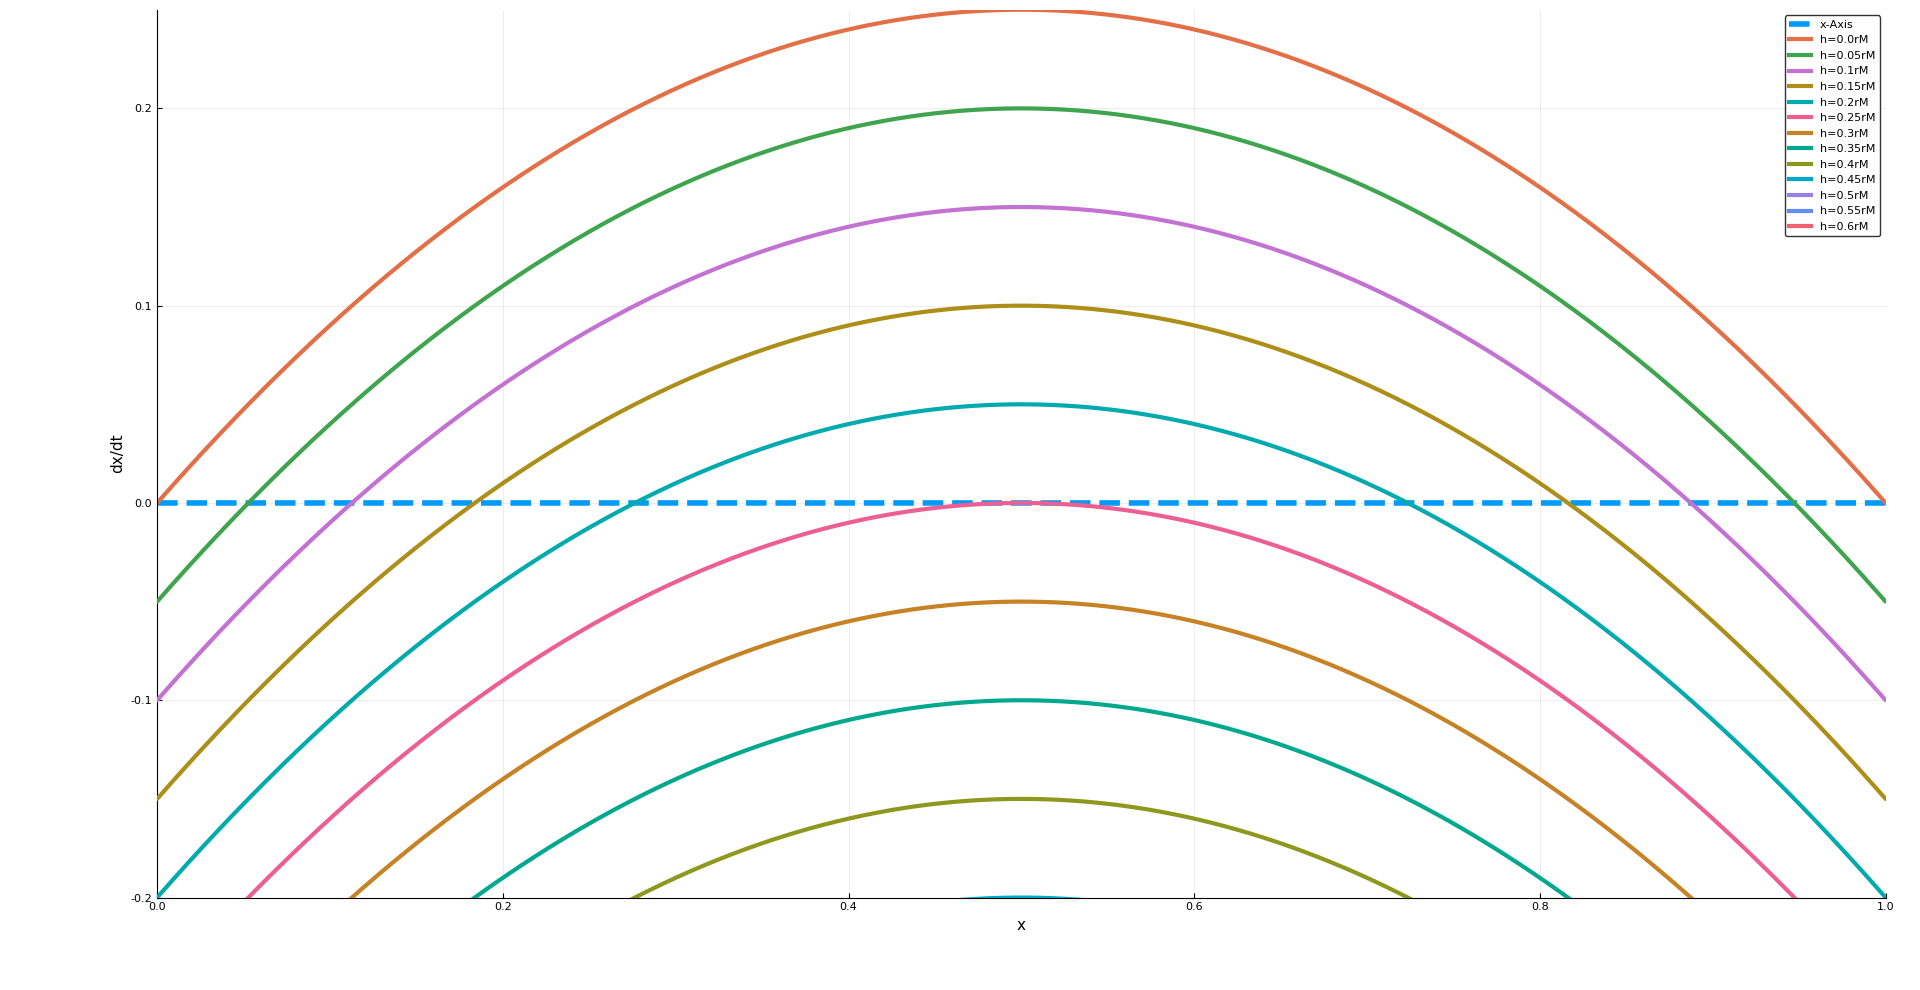
\includegraphics[width=0.8\textwidth]{CriticalPoints.png}
	\caption{Figure representing $\dev{x}{t}$ with different harvesting rates.}
	\label{fig: CriticalPoints}
\end{figure}
\begin{figure}
		\centering
		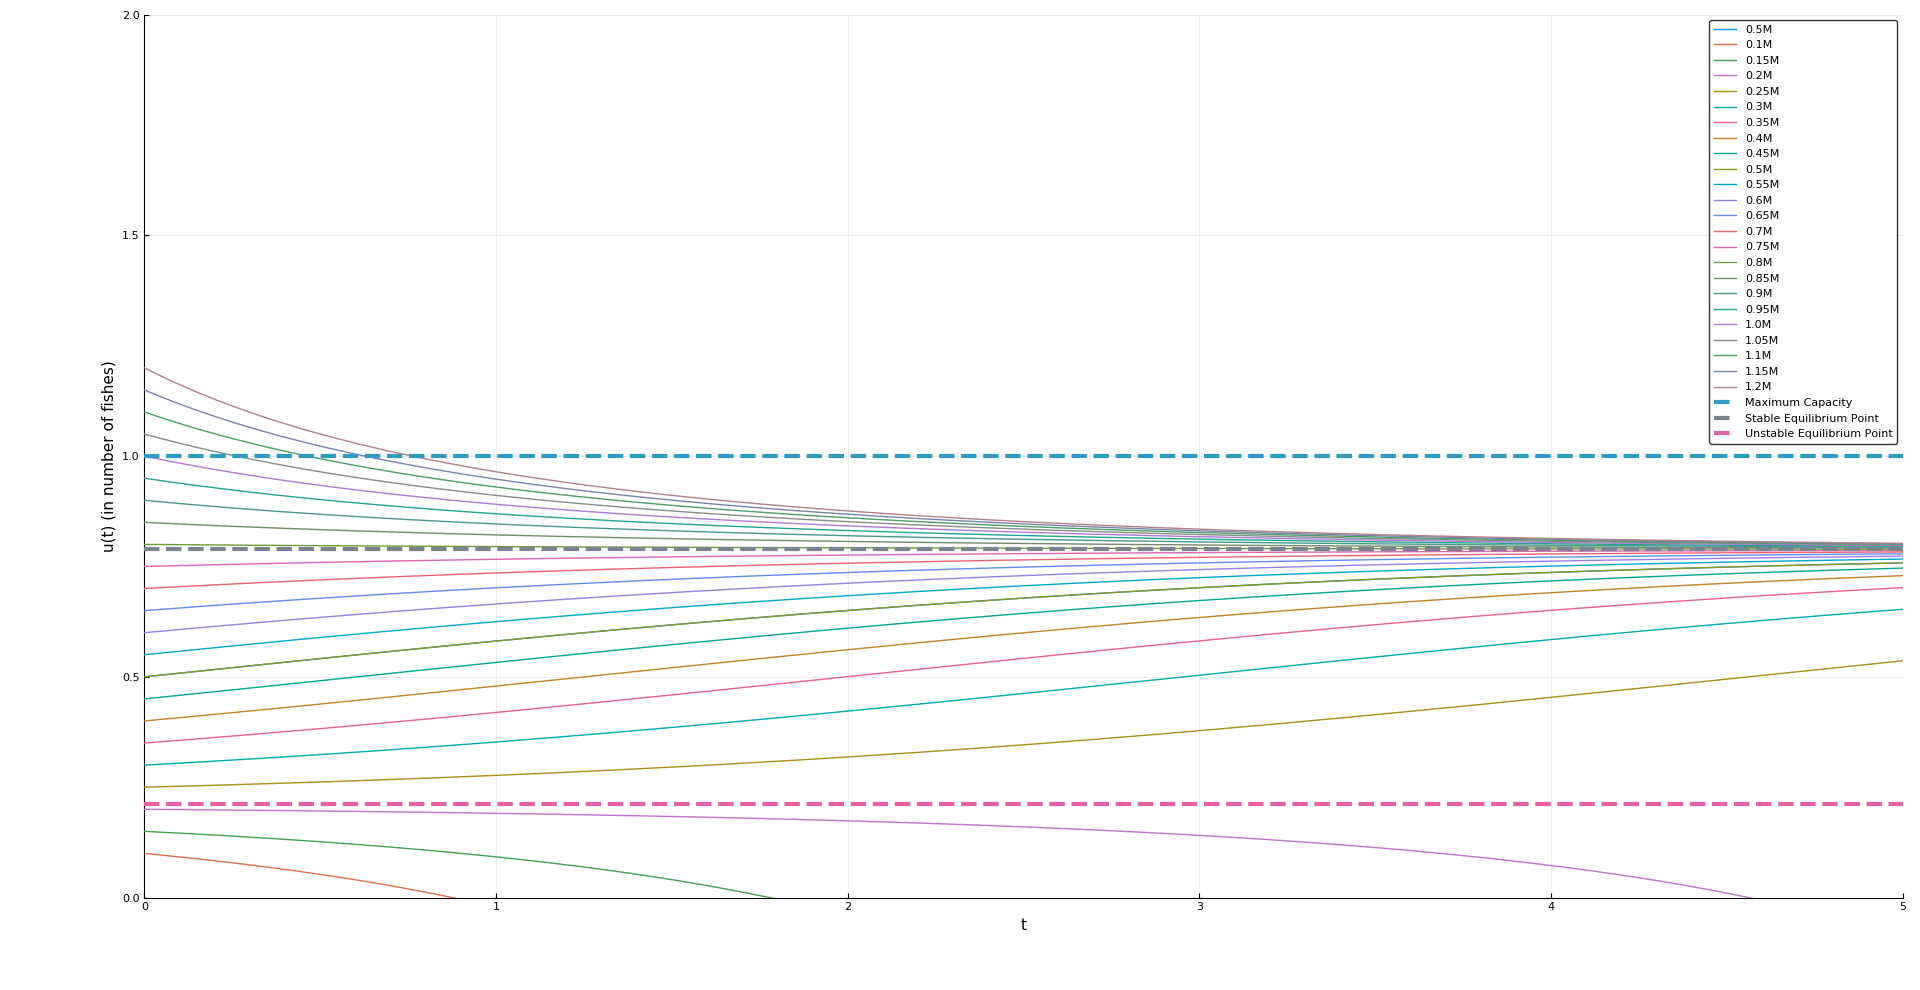
\includegraphics[width=0.8\textwidth]{SustainableConstant.png}
		\caption{Constant harvest rate $u<\frac{rM}{4}$.}
		\label{fig: SustainableConstantHarvest}
\end{figure}
\begin{figure}
	\centering
	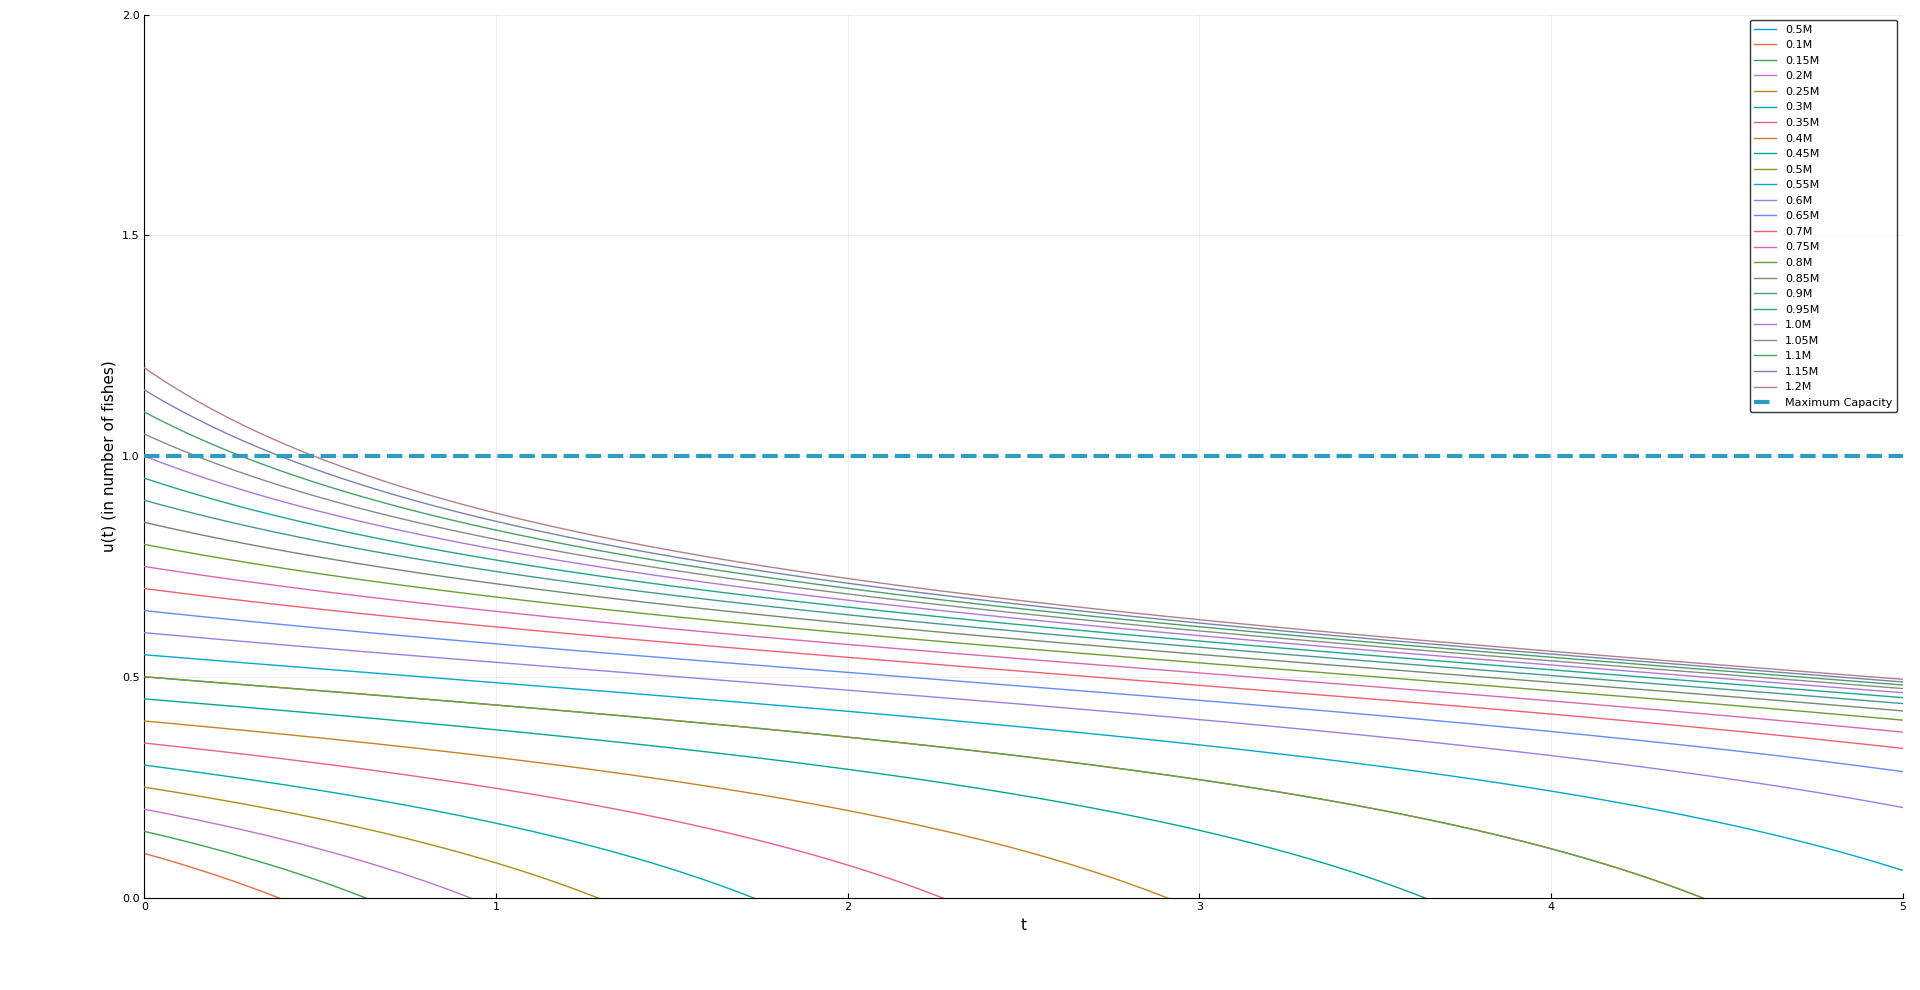
\includegraphics[width=0.8\textwidth]{OverExploitConstant.png}
	\caption{Constant harvest rate $u>\frac{rM}{4}$.}
	\label{fig: OverExploitConstantHarvest}
\end{figure}

\begin{figure}
	\centering
	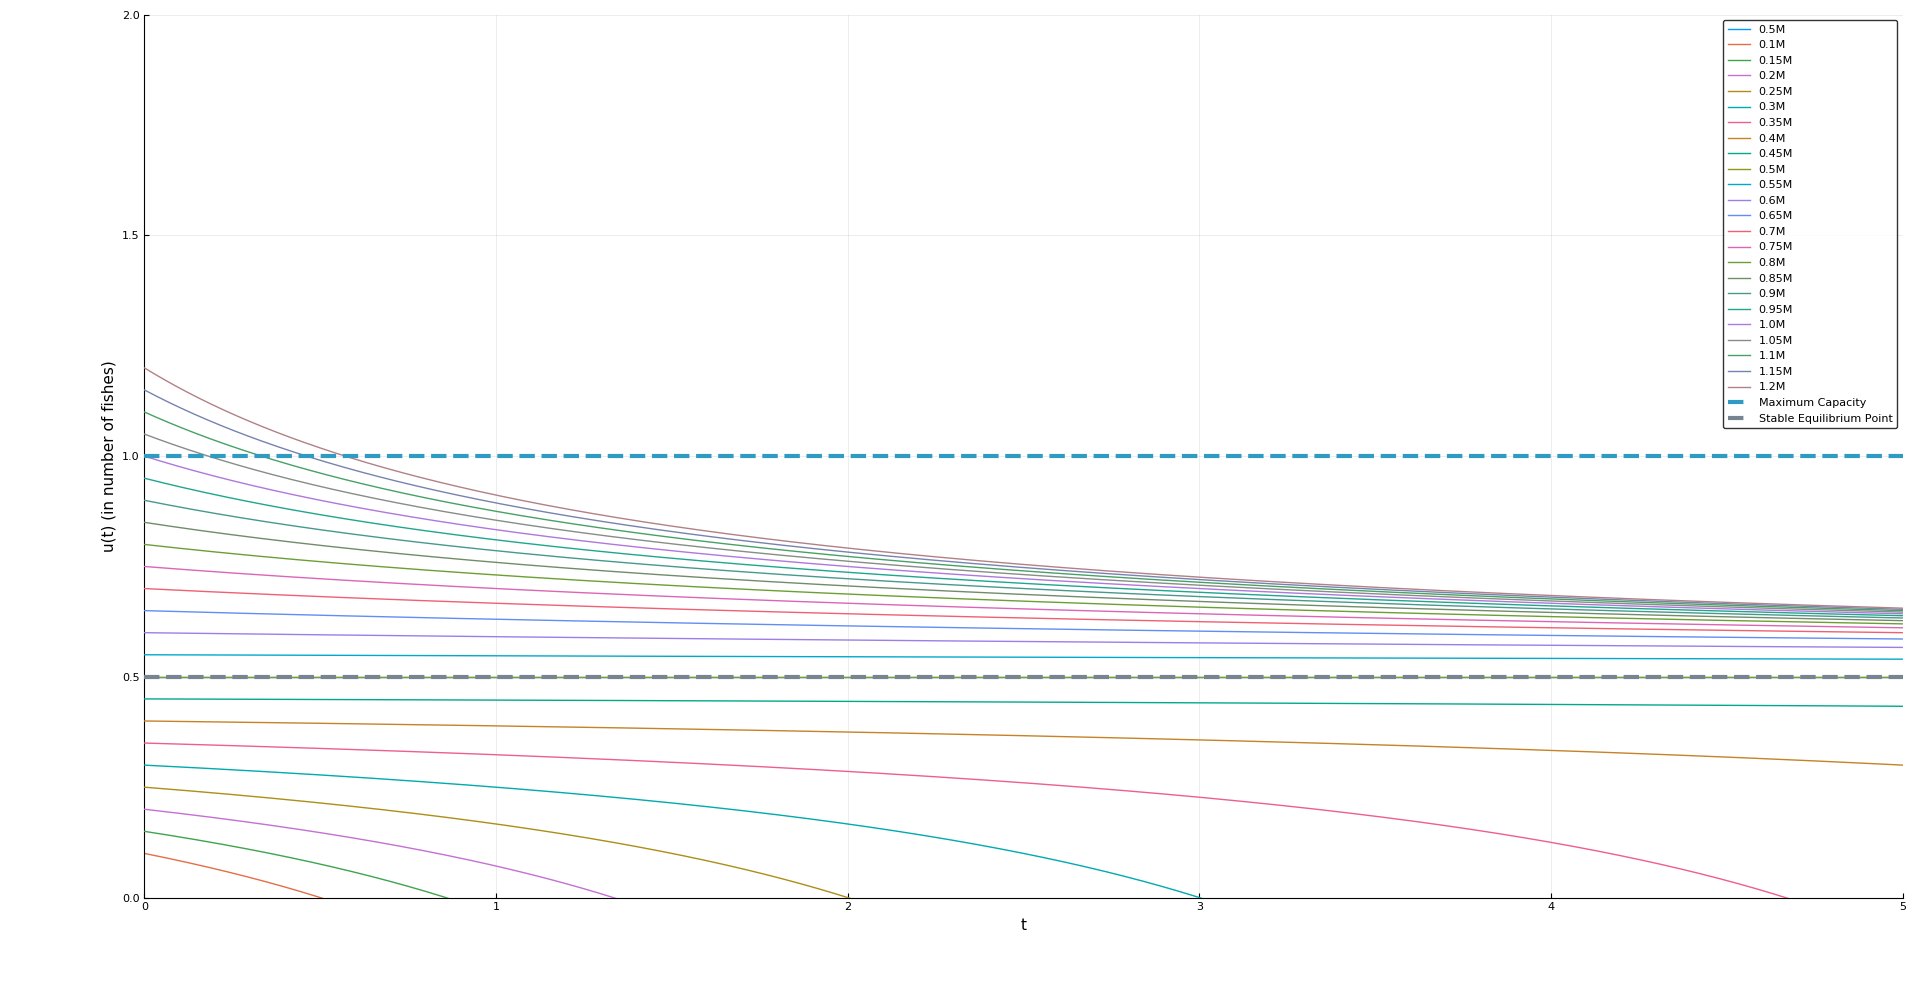
\includegraphics[width=0.8\textwidth]{CriticalExploitConstant.png}
	\caption{Constant harvest rate $u=\frac{rM}{4}$.}
	\label{fig: CriticalExploitConstantHarvest}
\end{figure}


		\subsection{Constant Harvesting Analysis.}
		\begin{equation}
\dev{x}{t}=rx\left(1-\frac{x}{M}\right)-u \label{eq: ConstantHarvest}
\end{equation}
We introduce the following variable in order to simply calculations,
\begin{equation}
\beta=\frac{uM}{r}
\end{equation}
Solving the differential equation,
\begin{align*}
	\frac{\diff{x}}{rx\left(1-\frac{x}{M}\right)-u}&=\diff{t} \\
	\int_{x_0}^{x}\frac{\diff{\chi}}{r\chi\left(1-\frac{\chi}{M}\right)-u}&=\int_{0}^{t}\diff{\tau} \\
	\frac{M}{r}\int_{x_0}^{x}\frac{\diff{\chi}}{\chi\left(M-\chi\right)-\frac{Mu}{r}}&=t \\
	-\frac{M}{r}\int_{x_0}^{x}\frac{\diff{\chi}}{\chi^2-M\chi+\beta}&=t \nonumber
	\end{align*}
Finally, we model the above integral as one 
\begin{align}
	-\frac{M}{r}\int_{x_0}^{x}\frac{\diff{\chi}}{\left(\chi-\frac{M}{2}\right)^2-\frac{M^2}{4}+\beta}&=t
\end{align}
Consider $\alpha$ as follows,
\begin{equation}
	\alpha = \beta - \frac{M^2}{4} = rM\left(u-\frac{rM}{4}\right)
\end{equation}
We see that the sign of $\alpha$ determines the nature of the solutions. Then, if $u>rM/4$ implies $\alpha>0$,
\begin{align*}
\int_{x_0}^{x}\frac{\diff{\chi}}{\left(\chi-\frac{M}{2}\right)^2+\alpha}&=-\frac{r}{M}t \\
\frac{1}{\sqrt{\beta-\frac{M^2}{4}}}\left(\arctan\left(\frac{x-M/2}{\sqrt{\beta-M^2/4}}\right)-\arctan\left(\frac{x_0-M/2}{\sqrt{\beta-M^2/4}}\right)\right)&=-\frac{r}{M}t \\
\end{align*}
Therefore, for $\alpha > 0$ the population behaves as follows, 
\begin{align}
	x(t)=\frac{M}{2}+\sqrt{\beta-\frac{M^2}{4}} \tan \left(\arctan\left(\frac{x_0-M/2}{\sqrt{\beta-M^2/4}}\right)-\frac{r\sqrt{\beta-M^2/4}}{M}t\right) \label{eq: ConstantHarvest OverExploit}
\end{align}

Equation \ref{eq: ConstantHarvest OverExploit} show us that for some $t^*$, $x(t^*)=0$,independently of the initial condition $x_0$, since the argument inside the $\tan$ is monotone decreasing in $t$. 

If $u<rM/4$ implies $-\alpha>0$,
\begin{align*}
	\int_{x_0}^{x}\frac{\diff{\chi}}{\left(\chi-\frac{M}{2}\right)^2-(-\alpha)} &=-\frac{r}{M}t
\end{align*}
Considering the zeros of the denominator, $\lambda$ and $\overleftarrow{\lambda}$, 
\begin{equation}
	\begin{array}{cc}
	\lambda&=\frac{M}{2}+\sqrt{\frac{M^2}{4}-\beta} \\
	\overline{\lambda}&=\frac{M}{2}-\sqrt{\frac{M^2}{4}-\beta} \\
	\end{array}
\end{equation}
We can rewrite our expression as follows, 
\begin{align*}
\int_{x_0}^{x} \left(\frac{1}{\chi - \lambda}-\frac{1}{\chi - \overline{\lambda}}\right)\diff{\chi} &=-\frac{2r\sqrt{M^2/4-\beta}}{M}t \\
	\ln\abs{\frac{x - \lambda}{x - \overline{\lambda}}}&=\ln\abs{\frac{x_0- \lambda}{x_0 - \overline{\lambda}}}-\frac{2r\sqrt{M^2/4-\beta}}{M}t
\end{align*}
For simplifying calculations, we write, $\gamma=\frac{2r\sqrt{M^2/4-\beta}}{M}$. And we obtain as result,
\begin{align}
\frac{x - \lambda}{x - \overline{\lambda}} &=\frac{x_0- \lambda}{x_0- \overline{\lambda}}\mathrm e^{-\gamma t} \\
x-\lambda &=\left(x-\overline{\lambda}\right)\left(\frac{x_0- \lambda}{x_0- \overline{\lambda}}\right)\mathrm e^{-\gamma t}
\end{align}

For the sake of simplicity, consider $\xi=\frac{x_0-\lambda}{x_0-\overline{\lambda}}\mathrm{e}^{-\gamma t}$. Therefore,
\begin{align*}
	x\left(1-\xi\right)&=\lambda-\overline{\lambda}\xi\\
	x&=\frac{\lambda-\overline{\lambda}\xi}{1-\xi} \\	
	x&=\frac{\frac{M}{2}+\sqrt{\frac{M^2}{4}-\beta}-\left(\frac{M}{2}-\sqrt{\frac{M^2}{4}-\beta}\right)\xi}{1-\xi}\\
	x&=\frac{\frac{M}{2}+\sqrt{\frac{M^2}{4}-\beta}-\left(\frac{M}{2}-\sqrt{\frac{M^2}{4}-\beta}\right)\xi}{1-\xi}\\
	x&=\frac{\frac{M}{2}\left(1-\xi\right)+\sqrt{\frac{M^2}{4}-\beta}\left(1+\xi\right)}{1-\xi}\\
	x&=\frac{M}{2}+\sqrt{\frac{M^2}{4}-\beta}\frac{1+\xi}{1-\xi}
\end{align*}
Hence, for $-\alpha>0$, we have the following result,
\begin{align}
	x(t)&=\frac{M}{2}+\left(\sqrt{\frac{M^2}{4}-\beta}\right)\frac{\left(x_0-M/2\right)\left(1+\mathrm e^{-\gamma t}\right)-\sqrt{M^2/4-\beta}\left(1-\mathrm{e}^{-\gamma t}\right)}{\left(x_0-M/2\right)\left(1-\mathrm e^{-\gamma t}\right)+\sqrt{M^2/4-\beta}\left(1+\mathrm{e}^{-\gamma t}\right)} \label{eq: Time Expression for Harvest}
\end{align}

If $u=\frac{rM}{4}$, we solve equation \ref{eq: ConstantHarvest} as follows,
\begin{align}
-\frac{M}{r}\int_{x_0}^{x}\frac{d\chi}{\left(\chi-\frac{M}{2}\right)^2}&=t\\
\int_{x_0}^{x}\frac{d\chi}{\left(\chi-\frac{M}{2}\right)^2}&=-\frac{rt}{M}\\
\frac{1}{x-\frac{M}{2}}&=\frac{1}{x_0-\frac{M}{2}}-\frac{rt}{M}\\
\frac{1}{x-\frac{M}{2}}&=\frac{M-\left(x_0-\frac{M}{2}\right)rt}{M\left(x_0-\frac{M}{2}\right)} \\
x&=\frac{M}{2}+\frac{M\left(x_0-\frac{M}{2}\right)}{M-\left(x_0-\frac{M}{2}\right)rt} 
\end{align}

The results above stated can be explained directly from the equation \ref{eq: ConstantHarvest}, as we see in the graph \ref{fig: CriticalPoints},  $F(x,t)$ is a paraboloid, with its maximum at $F(x^*=M/2,t)=rM^2/4$.

When $u=0$, we have the regular logistic equation with critical points $x_{c_1}=0$ and $x_{c_2}=M$. With $x_{c_2}$ being an stable fixed point and $x_{c_1}$ an unstable fixed point. In general, these are the solutions to the equation $F(x,t)-u=0$,
\begin{equation}
x_{c_{2,1}}=\frac{M}{2}\pm \sqrt{\frac{M^2}{4}-u\frac{M}{r}}
\end{equation}

We observe that the critical points $x_c$, such that $\dev{x_c}{t}=F(x_c, t)-u=0$ are getting closer to each other, as $u$ is increasing; when $u=\frac{rM}{4}$ we only have one critical unstable point. That behaves as an attractor when $x_0\geq\frac{M}{2}$. But when $x_0<\frac{M}{2}$ the population strictly decreases. For $u> \frac{rM}{4}$, the population $x(t)$ has no real critical points and the derivative $\dev{x}{t}$ is always negative, implying, that we will lead always the population to extinction, extracting constantly at a rate greater than $\frac{rM}{4}$.

\begin{figure}[H]
	\centering
	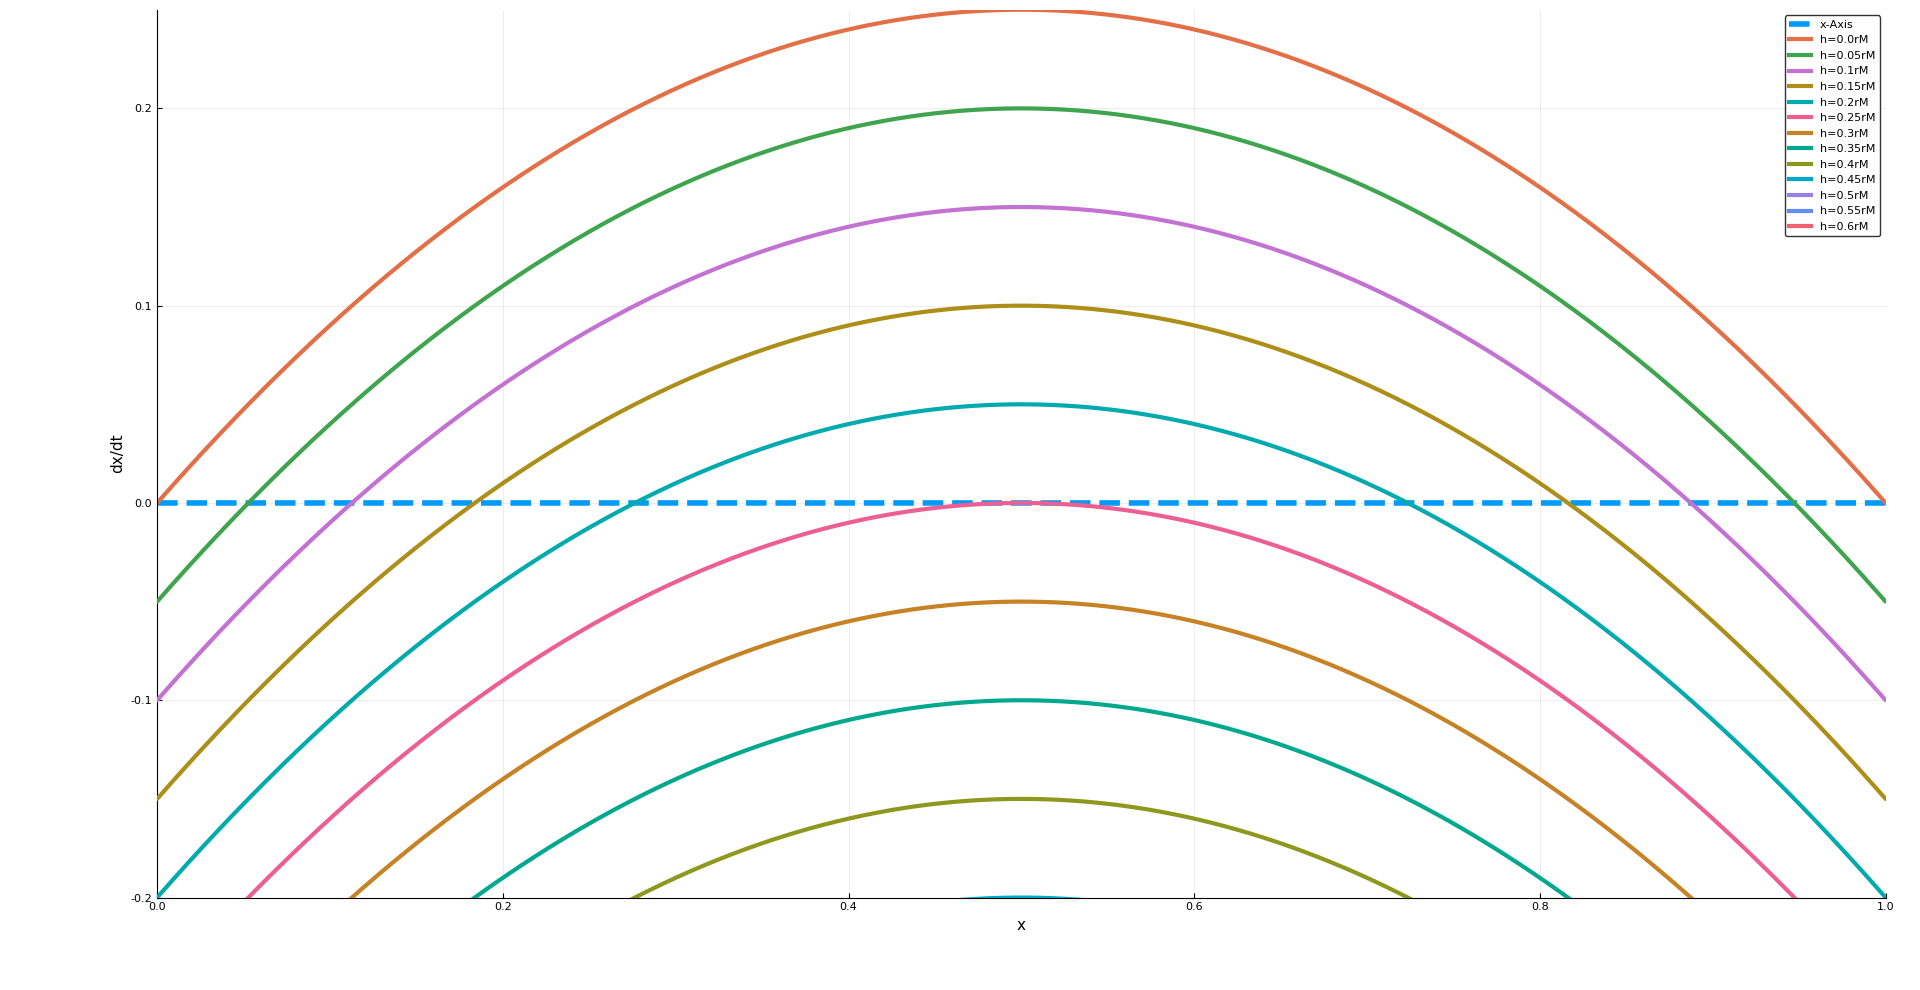
\includegraphics[width=0.8\textwidth]{CriticalPoints.png}
	\caption{Figure representing $\dev{x}{t}$ with different harvesting rates.}
	\label{fig: CriticalPoints}
\end{figure}
\begin{figure}
		\centering
		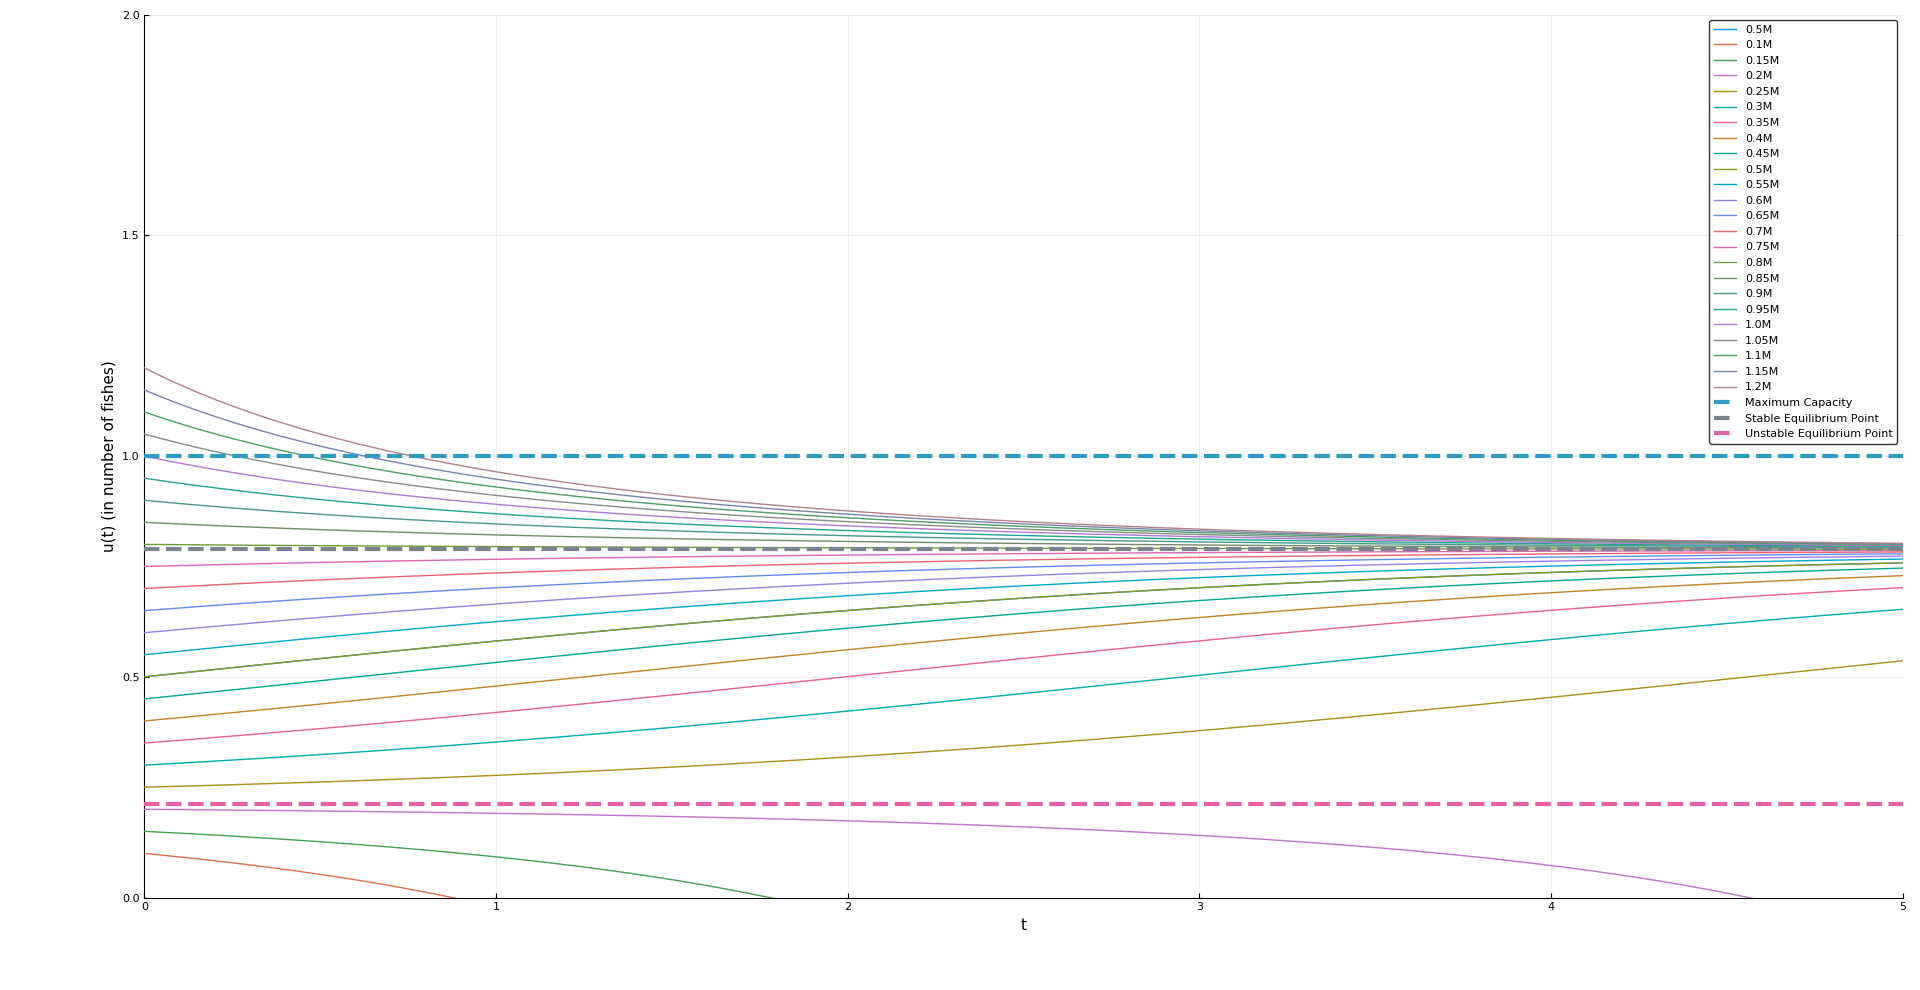
\includegraphics[width=0.8\textwidth]{SustainableConstant.png}
		\caption{Constant harvest rate $u<\frac{rM}{4}$.}
		\label{fig: SustainableConstantHarvest}
\end{figure}
\begin{figure}
	\centering
	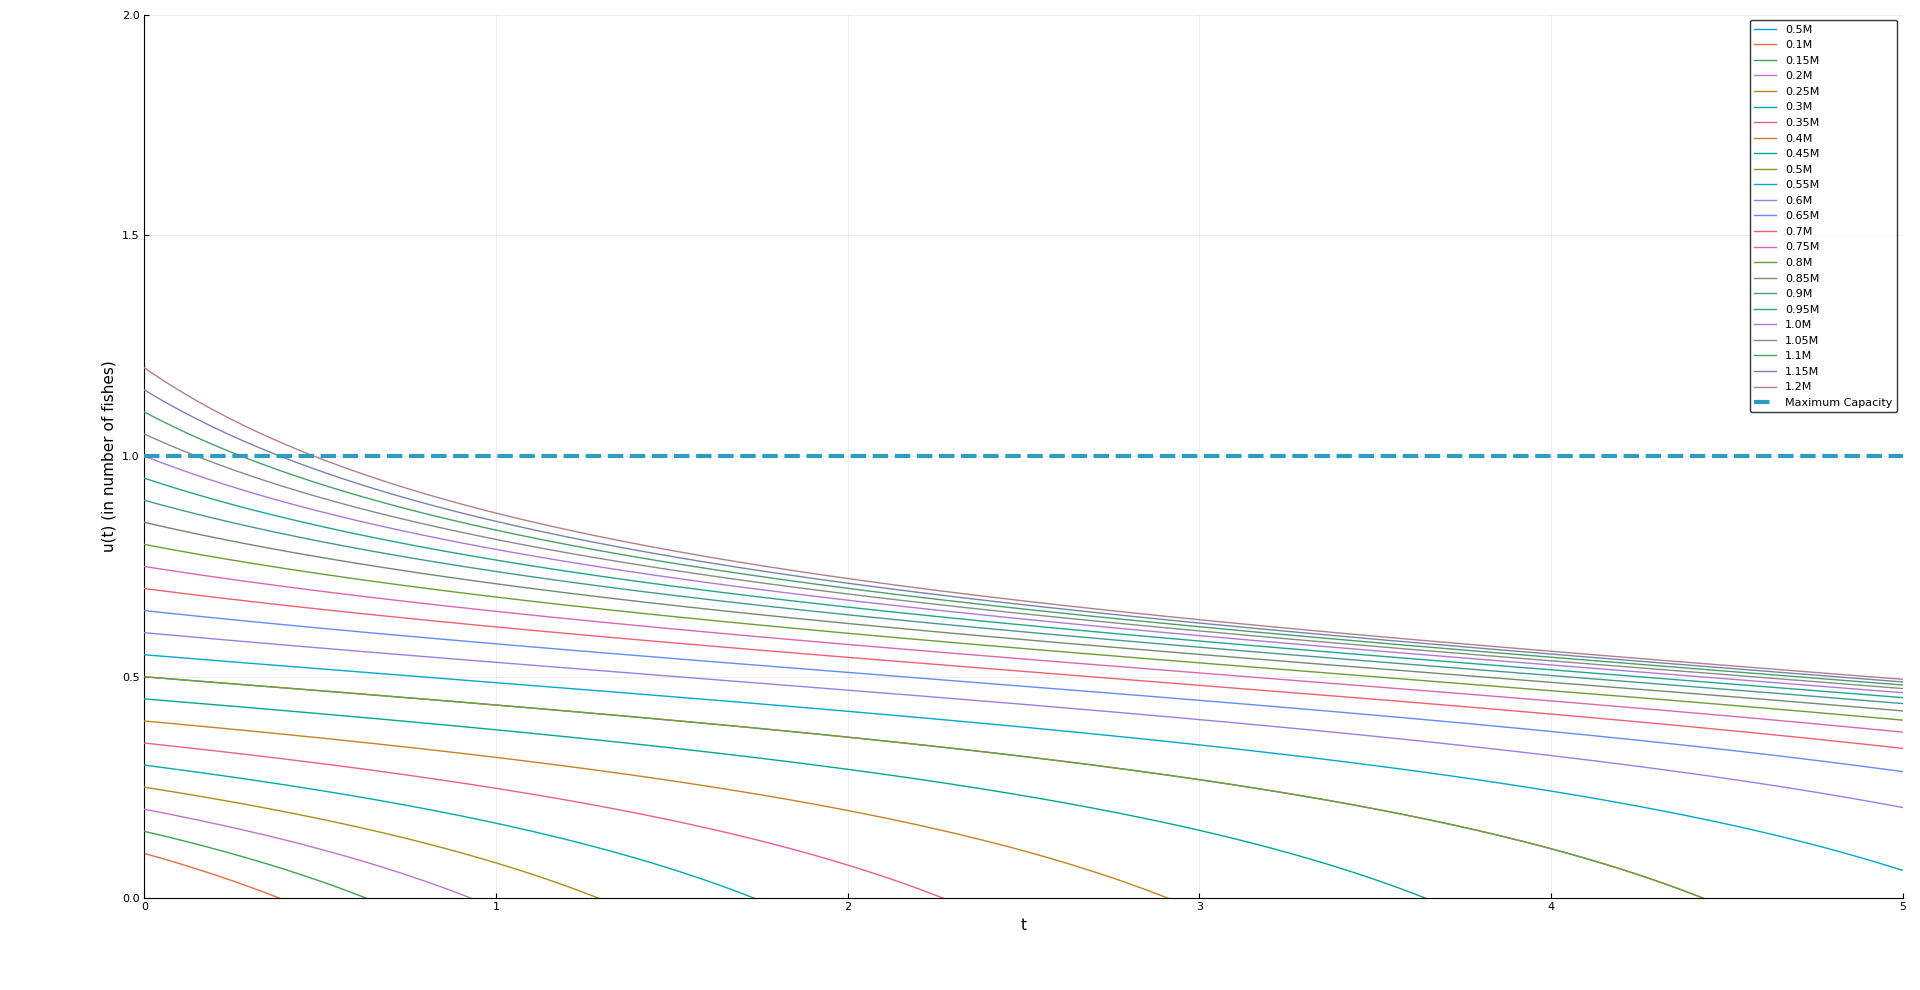
\includegraphics[width=0.8\textwidth]{OverExploitConstant.png}
	\caption{Constant harvest rate $u>\frac{rM}{4}$.}
	\label{fig: OverExploitConstantHarvest}
\end{figure}

\begin{figure}
	\centering
	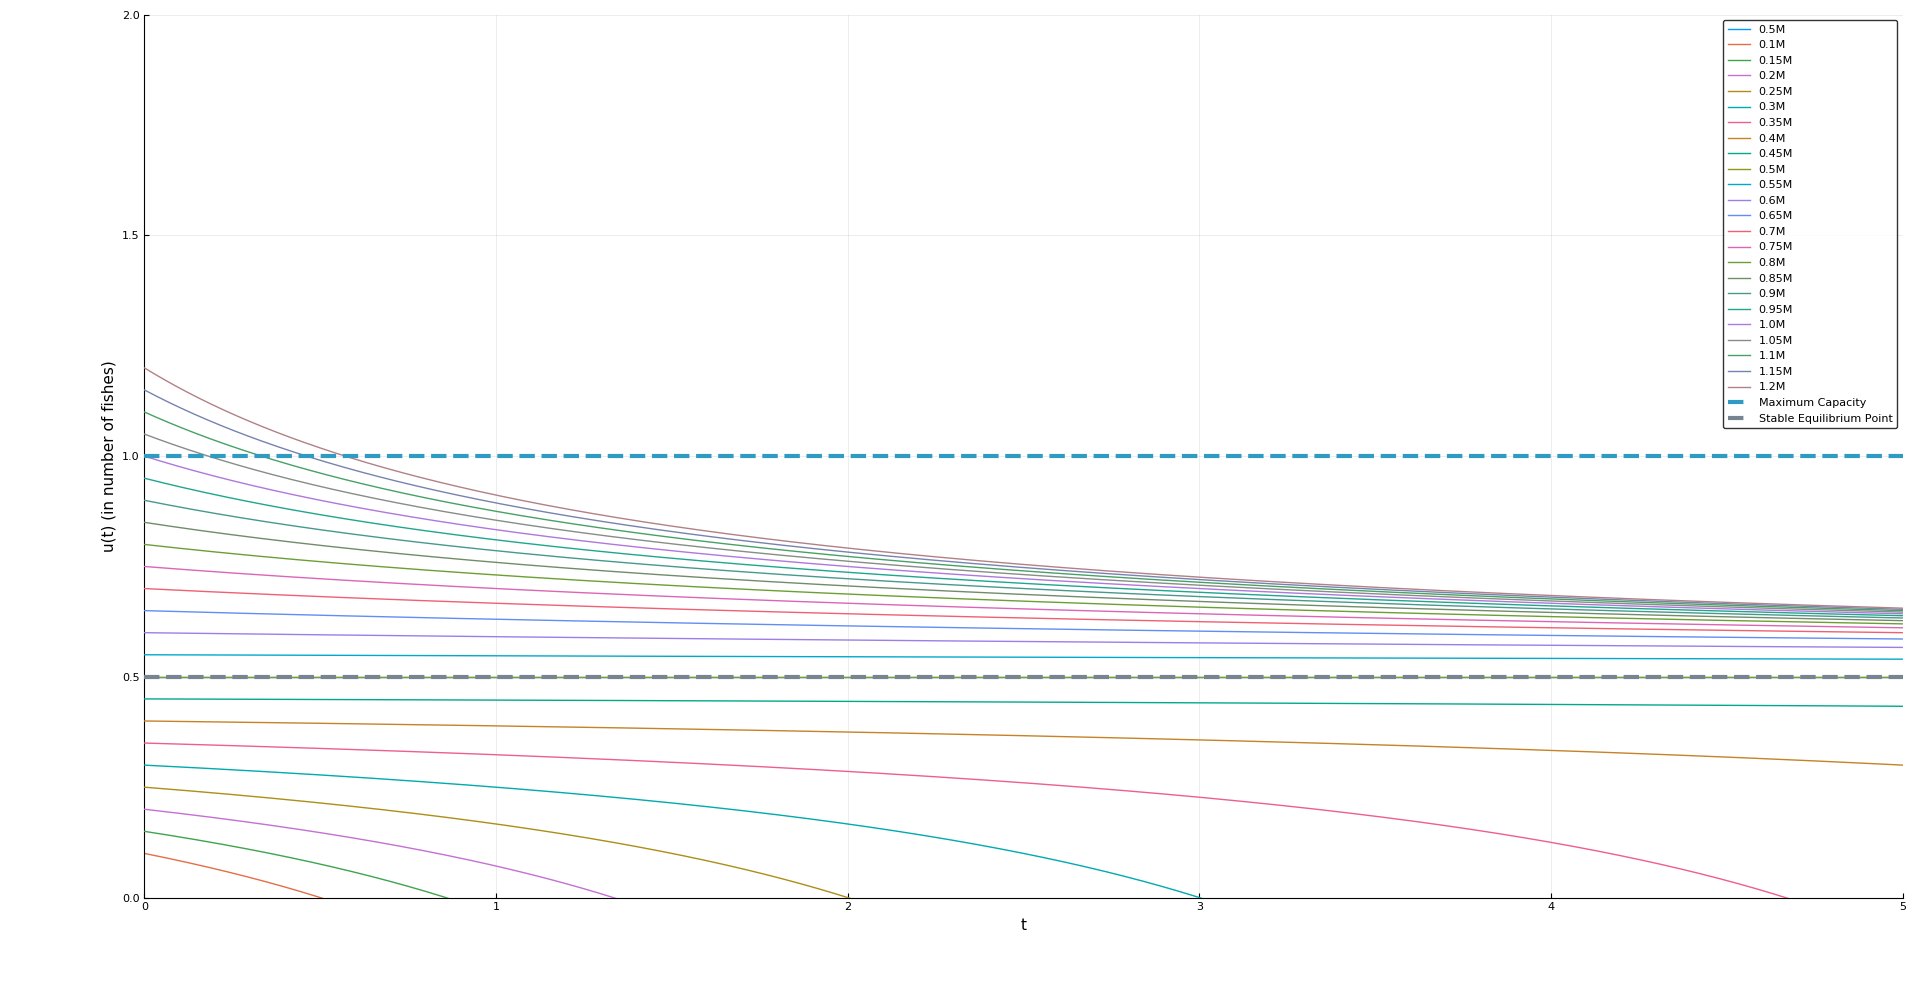
\includegraphics[width=0.8\textwidth]{CriticalExploitConstant.png}
	\caption{Constant harvest rate $u=\frac{rM}{4}$.}
	\label{fig: CriticalExploitConstantHarvest}
\end{figure}


		\subsection{Time Varying Harvesting.}
		\begin{equation}
\dev{x}{t}=rx\left(1-\frac{x}{M}\right)-u \label{eq: ConstantHarvest}
\end{equation}
We introduce the following variable in order to simply calculations,
\begin{equation}
\beta=\frac{uM}{r}
\end{equation}
Solving the differential equation,
\begin{align*}
	\frac{\diff{x}}{rx\left(1-\frac{x}{M}\right)-u}&=\diff{t} \\
	\int_{x_0}^{x}\frac{\diff{\chi}}{r\chi\left(1-\frac{\chi}{M}\right)-u}&=\int_{0}^{t}\diff{\tau} \\
	\frac{M}{r}\int_{x_0}^{x}\frac{\diff{\chi}}{\chi\left(M-\chi\right)-\frac{Mu}{r}}&=t \\
	-\frac{M}{r}\int_{x_0}^{x}\frac{\diff{\chi}}{\chi^2-M\chi+\beta}&=t \nonumber
	\end{align*}
Finally, we model the above integral as one 
\begin{align}
	-\frac{M}{r}\int_{x_0}^{x}\frac{\diff{\chi}}{\left(\chi-\frac{M}{2}\right)^2-\frac{M^2}{4}+\beta}&=t
\end{align}
Consider $\alpha$ as follows,
\begin{equation}
	\alpha = \beta - \frac{M^2}{4} = rM\left(u-\frac{rM}{4}\right)
\end{equation}
We see that the sign of $\alpha$ determines the nature of the solutions. Then, if $u>rM/4$ implies $\alpha>0$,
\begin{align*}
\int_{x_0}^{x}\frac{\diff{\chi}}{\left(\chi-\frac{M}{2}\right)^2+\alpha}&=-\frac{r}{M}t \\
\frac{1}{\sqrt{\beta-\frac{M^2}{4}}}\left(\arctan\left(\frac{x-M/2}{\sqrt{\beta-M^2/4}}\right)-\arctan\left(\frac{x_0-M/2}{\sqrt{\beta-M^2/4}}\right)\right)&=-\frac{r}{M}t \\
\end{align*}
Therefore, for $\alpha > 0$ the population behaves as follows, 
\begin{align}
	x(t)=\frac{M}{2}+\sqrt{\beta-\frac{M^2}{4}} \tan \left(\arctan\left(\frac{x_0-M/2}{\sqrt{\beta-M^2/4}}\right)-\frac{r\sqrt{\beta-M^2/4}}{M}t\right) \label{eq: ConstantHarvest OverExploit}
\end{align}

Equation \ref{eq: ConstantHarvest OverExploit} show us that for some $t^*$, $x(t^*)=0$,independently of the initial condition $x_0$, since the argument inside the $\tan$ is monotone decreasing in $t$. 

If $u<rM/4$ implies $-\alpha>0$,
\begin{align*}
	\int_{x_0}^{x}\frac{\diff{\chi}}{\left(\chi-\frac{M}{2}\right)^2-(-\alpha)} &=-\frac{r}{M}t
\end{align*}
Considering the zeros of the denominator, $\lambda$ and $\overleftarrow{\lambda}$, 
\begin{equation}
	\begin{array}{cc}
	\lambda&=\frac{M}{2}+\sqrt{\frac{M^2}{4}-\beta} \\
	\overline{\lambda}&=\frac{M}{2}-\sqrt{\frac{M^2}{4}-\beta} \\
	\end{array}
\end{equation}
We can rewrite our expression as follows, 
\begin{align*}
\int_{x_0}^{x} \left(\frac{1}{\chi - \lambda}-\frac{1}{\chi - \overline{\lambda}}\right)\diff{\chi} &=-\frac{2r\sqrt{M^2/4-\beta}}{M}t \\
	\ln\abs{\frac{x - \lambda}{x - \overline{\lambda}}}&=\ln\abs{\frac{x_0- \lambda}{x_0 - \overline{\lambda}}}-\frac{2r\sqrt{M^2/4-\beta}}{M}t
\end{align*}
For simplifying calculations, we write, $\gamma=\frac{2r\sqrt{M^2/4-\beta}}{M}$. And we obtain as result,
\begin{align}
\frac{x - \lambda}{x - \overline{\lambda}} &=\frac{x_0- \lambda}{x_0- \overline{\lambda}}\mathrm e^{-\gamma t} \\
x-\lambda &=\left(x-\overline{\lambda}\right)\left(\frac{x_0- \lambda}{x_0- \overline{\lambda}}\right)\mathrm e^{-\gamma t}
\end{align}

For the sake of simplicity, consider $\xi=\frac{x_0-\lambda}{x_0-\overline{\lambda}}\mathrm{e}^{-\gamma t}$. Therefore,
\begin{align*}
	x\left(1-\xi\right)&=\lambda-\overline{\lambda}\xi\\
	x&=\frac{\lambda-\overline{\lambda}\xi}{1-\xi} \\	
	x&=\frac{\frac{M}{2}+\sqrt{\frac{M^2}{4}-\beta}-\left(\frac{M}{2}-\sqrt{\frac{M^2}{4}-\beta}\right)\xi}{1-\xi}\\
	x&=\frac{\frac{M}{2}+\sqrt{\frac{M^2}{4}-\beta}-\left(\frac{M}{2}-\sqrt{\frac{M^2}{4}-\beta}\right)\xi}{1-\xi}\\
	x&=\frac{\frac{M}{2}\left(1-\xi\right)+\sqrt{\frac{M^2}{4}-\beta}\left(1+\xi\right)}{1-\xi}\\
	x&=\frac{M}{2}+\sqrt{\frac{M^2}{4}-\beta}\frac{1+\xi}{1-\xi}
\end{align*}
Hence, for $-\alpha>0$, we have the following result,
\begin{align}
	x(t)&=\frac{M}{2}+\left(\sqrt{\frac{M^2}{4}-\beta}\right)\frac{\left(x_0-M/2\right)\left(1+\mathrm e^{-\gamma t}\right)-\sqrt{M^2/4-\beta}\left(1-\mathrm{e}^{-\gamma t}\right)}{\left(x_0-M/2\right)\left(1-\mathrm e^{-\gamma t}\right)+\sqrt{M^2/4-\beta}\left(1+\mathrm{e}^{-\gamma t}\right)} \label{eq: Time Expression for Harvest}
\end{align}

If $u=\frac{rM}{4}$, we solve equation \ref{eq: ConstantHarvest} as follows,
\begin{align}
-\frac{M}{r}\int_{x_0}^{x}\frac{d\chi}{\left(\chi-\frac{M}{2}\right)^2}&=t\\
\int_{x_0}^{x}\frac{d\chi}{\left(\chi-\frac{M}{2}\right)^2}&=-\frac{rt}{M}\\
\frac{1}{x-\frac{M}{2}}&=\frac{1}{x_0-\frac{M}{2}}-\frac{rt}{M}\\
\frac{1}{x-\frac{M}{2}}&=\frac{M-\left(x_0-\frac{M}{2}\right)rt}{M\left(x_0-\frac{M}{2}\right)} \\
x&=\frac{M}{2}+\frac{M\left(x_0-\frac{M}{2}\right)}{M-\left(x_0-\frac{M}{2}\right)rt} 
\end{align}

The results above stated can be explained directly from the equation \ref{eq: ConstantHarvest}, as we see in the graph \ref{fig: CriticalPoints},  $F(x,t)$ is a paraboloid, with its maximum at $F(x^*=M/2,t)=rM^2/4$.

When $u=0$, we have the regular logistic equation with critical points $x_{c_1}=0$ and $x_{c_2}=M$. With $x_{c_2}$ being an stable fixed point and $x_{c_1}$ an unstable fixed point. In general, these are the solutions to the equation $F(x,t)-u=0$,
\begin{equation}
x_{c_{2,1}}=\frac{M}{2}\pm \sqrt{\frac{M^2}{4}-u\frac{M}{r}}
\end{equation}

We observe that the critical points $x_c$, such that $\dev{x_c}{t}=F(x_c, t)-u=0$ are getting closer to each other, as $u$ is increasing; when $u=\frac{rM}{4}$ we only have one critical unstable point. That behaves as an attractor when $x_0\geq\frac{M}{2}$. But when $x_0<\frac{M}{2}$ the population strictly decreases. For $u> \frac{rM}{4}$, the population $x(t)$ has no real critical points and the derivative $\dev{x}{t}$ is always negative, implying, that we will lead always the population to extinction, extracting constantly at a rate greater than $\frac{rM}{4}$.

\begin{figure}[H]
	\centering
	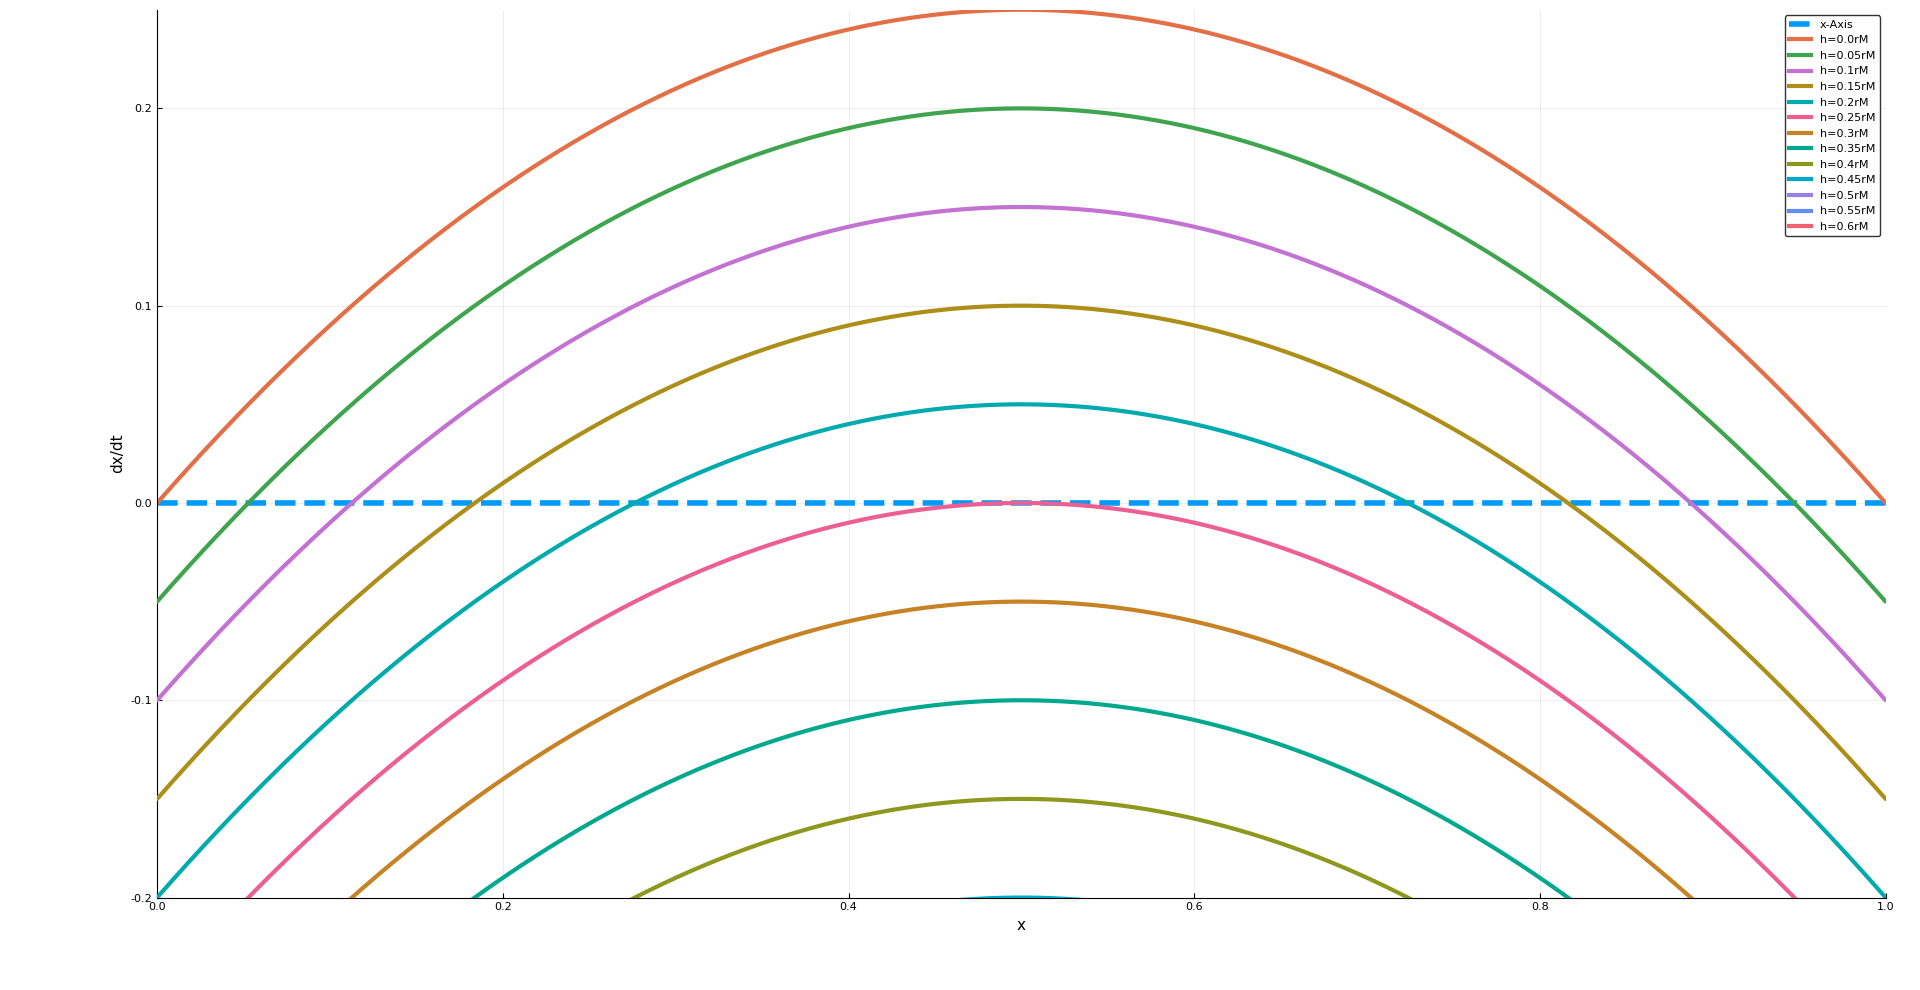
\includegraphics[width=0.8\textwidth]{CriticalPoints.png}
	\caption{Figure representing $\dev{x}{t}$ with different harvesting rates.}
	\label{fig: CriticalPoints}
\end{figure}
\begin{figure}
		\centering
		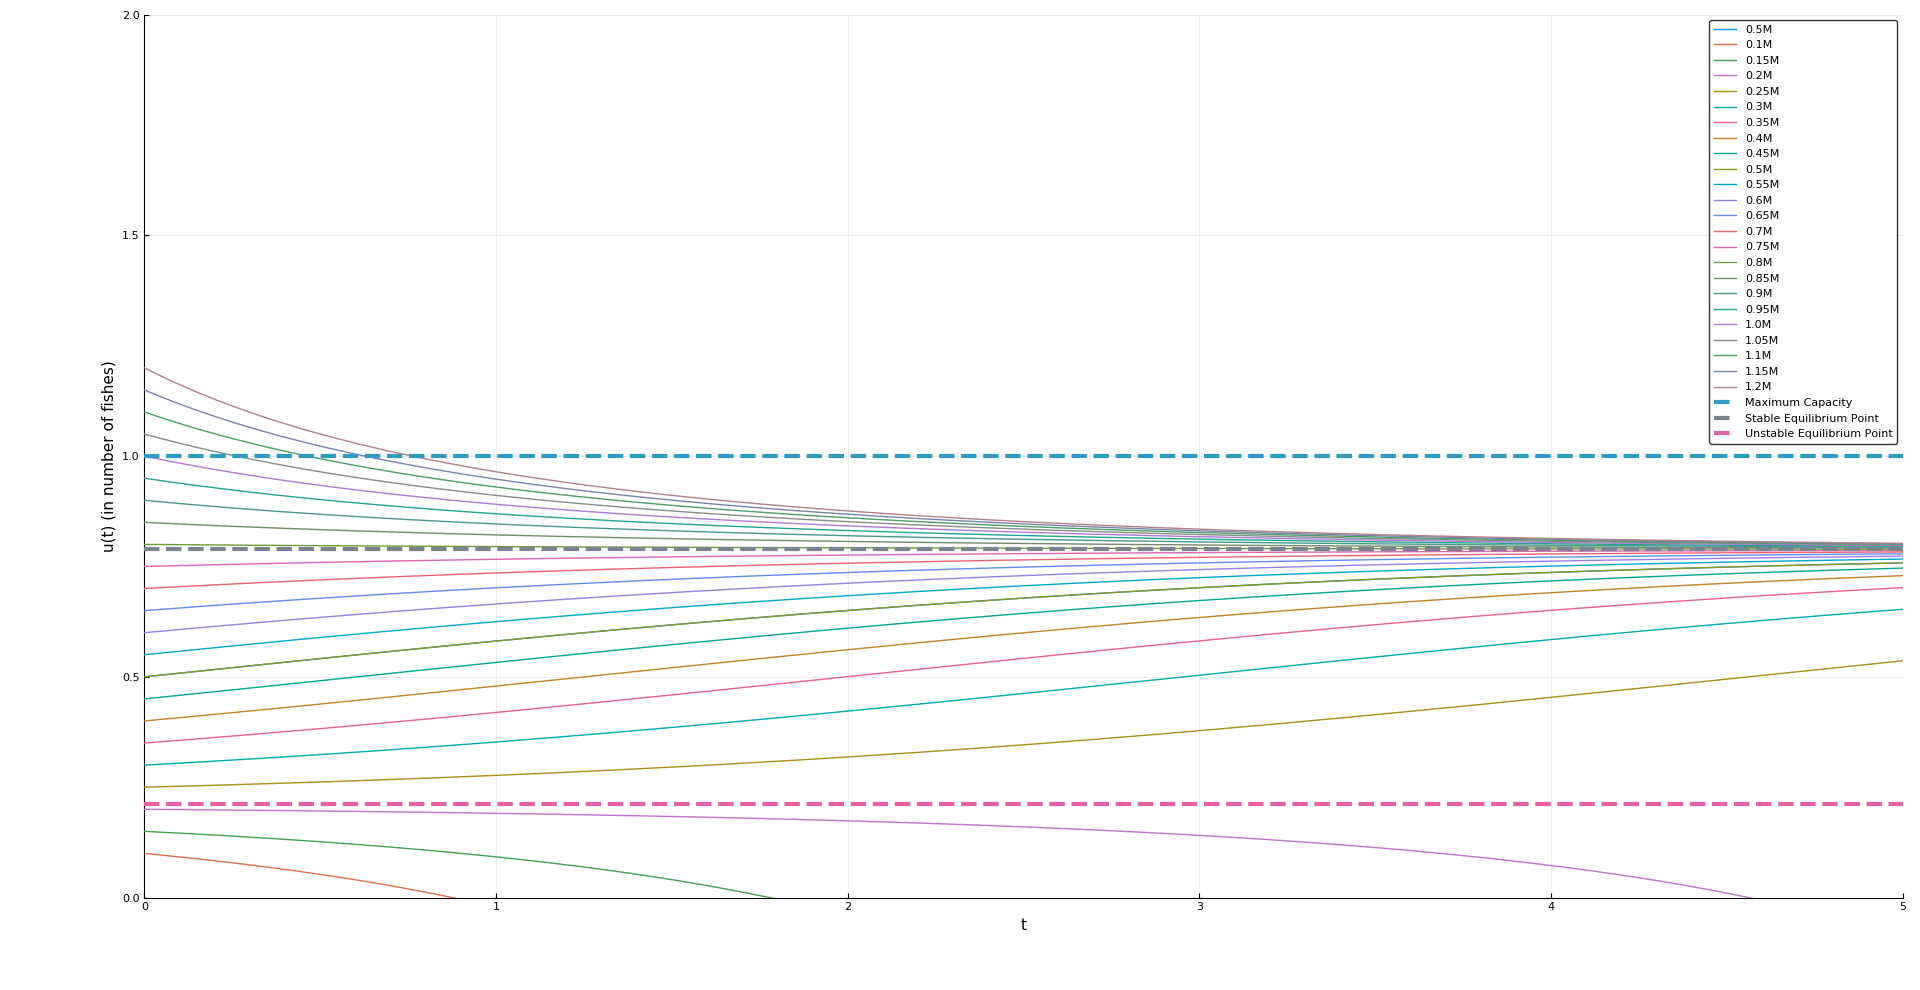
\includegraphics[width=0.8\textwidth]{SustainableConstant.png}
		\caption{Constant harvest rate $u<\frac{rM}{4}$.}
		\label{fig: SustainableConstantHarvest}
\end{figure}
\begin{figure}
	\centering
	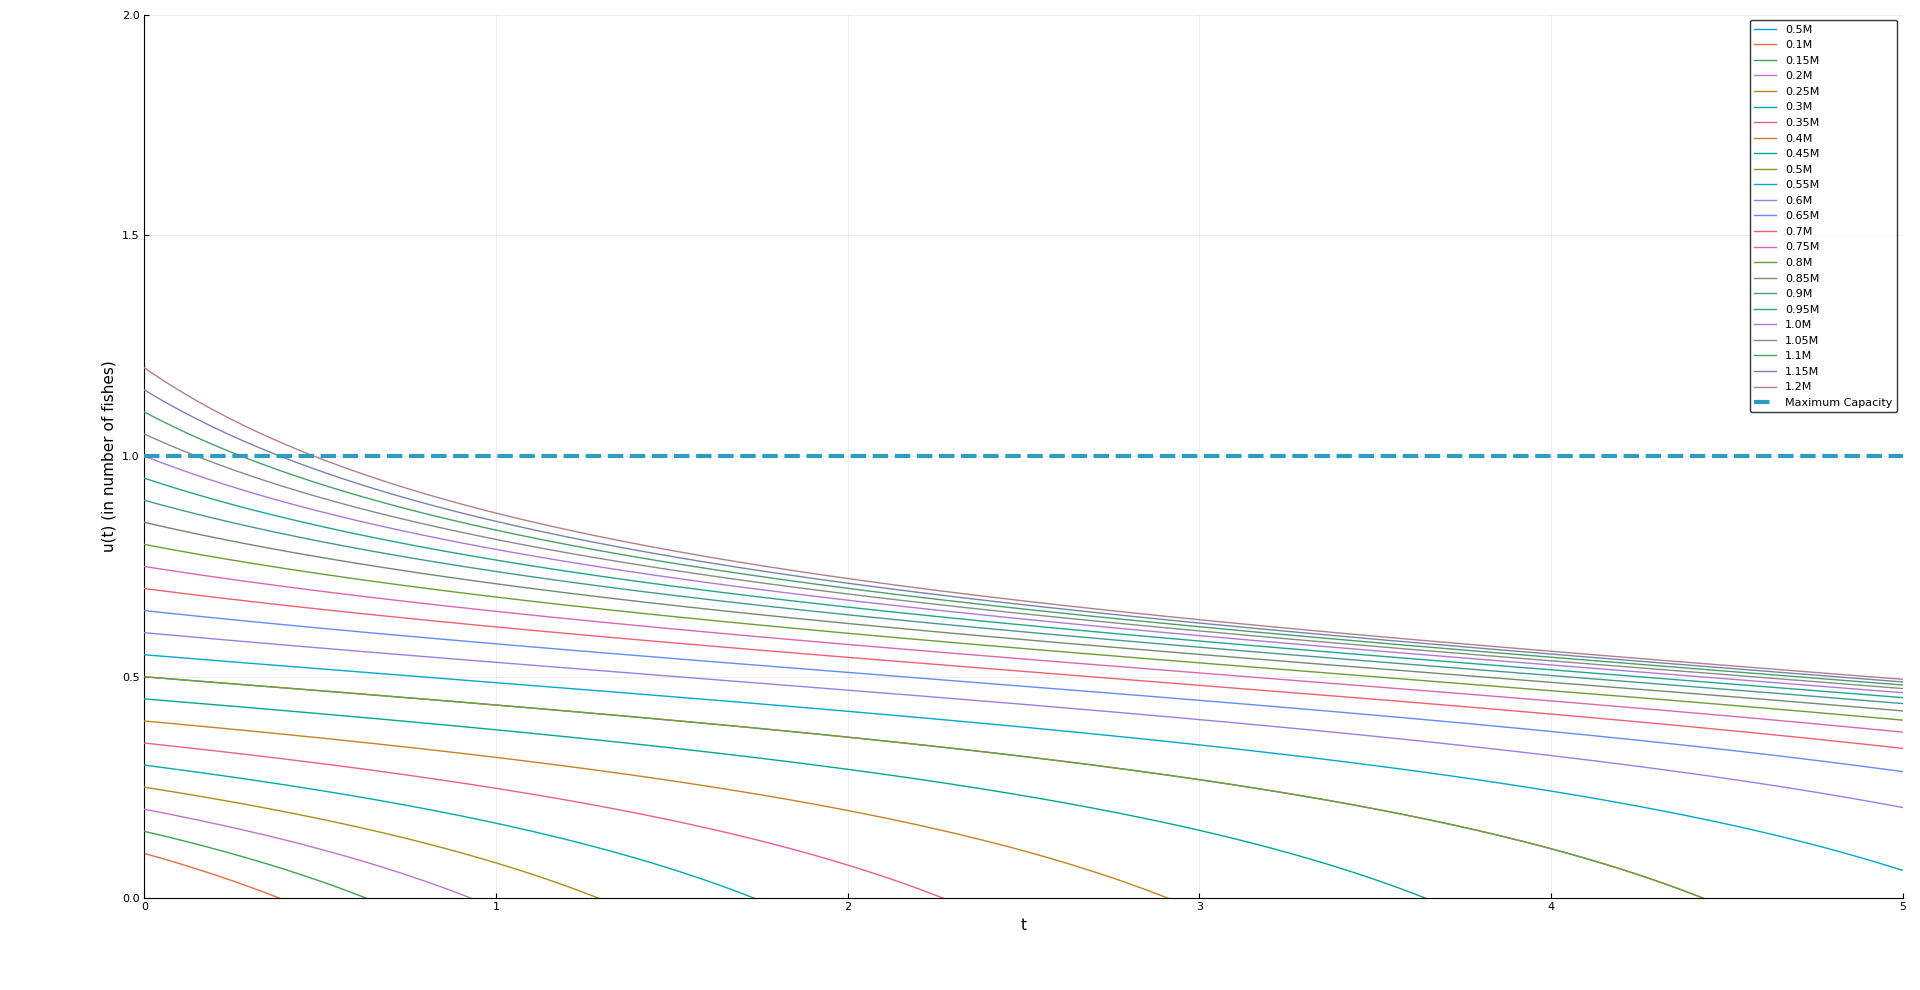
\includegraphics[width=0.8\textwidth]{OverExploitConstant.png}
	\caption{Constant harvest rate $u>\frac{rM}{4}$.}
	\label{fig: OverExploitConstantHarvest}
\end{figure}

\begin{figure}
	\centering
	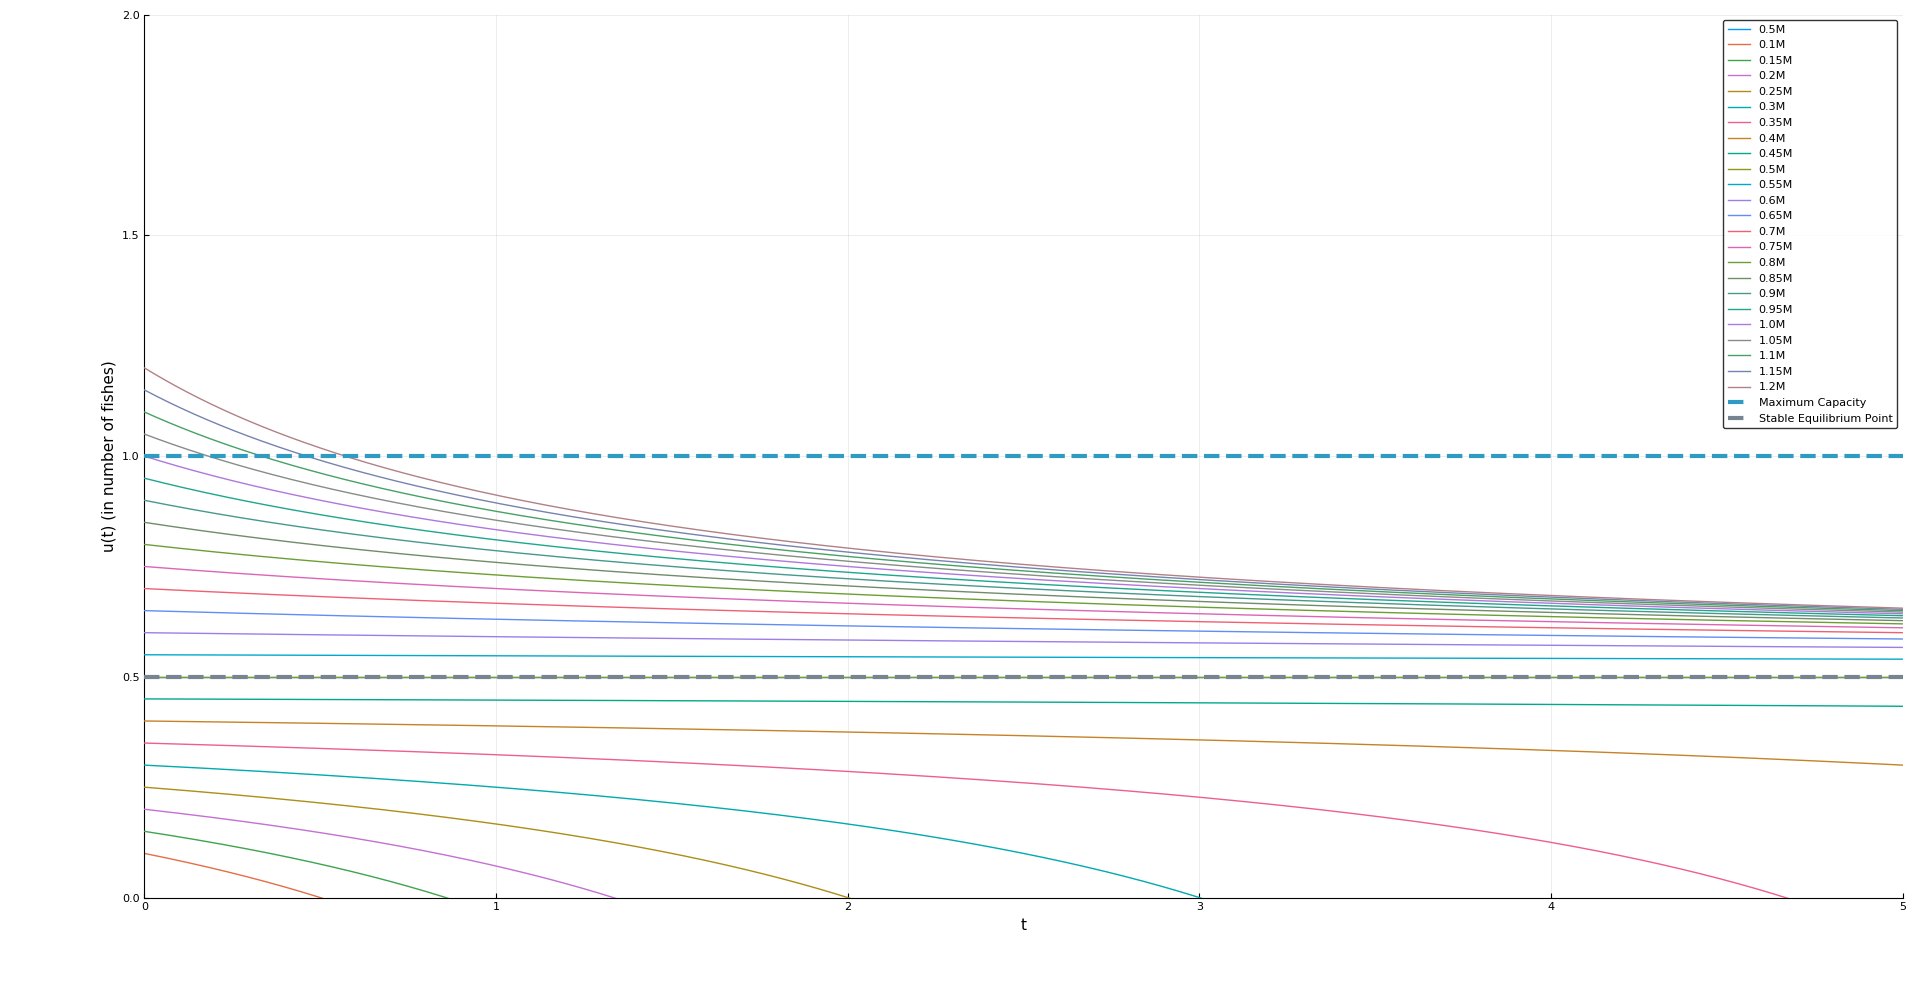
\includegraphics[width=0.8\textwidth]{CriticalExploitConstant.png}
	\caption{Constant harvest rate $u=\frac{rM}{4}$.}
	\label{fig: CriticalExploitConstantHarvest}
\end{figure}


		\subsection{Optimal Harvesting. Smooth Optimal Control Problem.}
		\begin{equation}
\dev{x}{t}=rx\left(1-\frac{x}{M}\right)-u \label{eq: ConstantHarvest}
\end{equation}
We introduce the following variable in order to simply calculations,
\begin{equation}
\beta=\frac{uM}{r}
\end{equation}
Solving the differential equation,
\begin{align*}
	\frac{\diff{x}}{rx\left(1-\frac{x}{M}\right)-u}&=\diff{t} \\
	\int_{x_0}^{x}\frac{\diff{\chi}}{r\chi\left(1-\frac{\chi}{M}\right)-u}&=\int_{0}^{t}\diff{\tau} \\
	\frac{M}{r}\int_{x_0}^{x}\frac{\diff{\chi}}{\chi\left(M-\chi\right)-\frac{Mu}{r}}&=t \\
	-\frac{M}{r}\int_{x_0}^{x}\frac{\diff{\chi}}{\chi^2-M\chi+\beta}&=t \nonumber
	\end{align*}
Finally, we model the above integral as one 
\begin{align}
	-\frac{M}{r}\int_{x_0}^{x}\frac{\diff{\chi}}{\left(\chi-\frac{M}{2}\right)^2-\frac{M^2}{4}+\beta}&=t
\end{align}
Consider $\alpha$ as follows,
\begin{equation}
	\alpha = \beta - \frac{M^2}{4} = rM\left(u-\frac{rM}{4}\right)
\end{equation}
We see that the sign of $\alpha$ determines the nature of the solutions. Then, if $u>rM/4$ implies $\alpha>0$,
\begin{align*}
\int_{x_0}^{x}\frac{\diff{\chi}}{\left(\chi-\frac{M}{2}\right)^2+\alpha}&=-\frac{r}{M}t \\
\frac{1}{\sqrt{\beta-\frac{M^2}{4}}}\left(\arctan\left(\frac{x-M/2}{\sqrt{\beta-M^2/4}}\right)-\arctan\left(\frac{x_0-M/2}{\sqrt{\beta-M^2/4}}\right)\right)&=-\frac{r}{M}t \\
\end{align*}
Therefore, for $\alpha > 0$ the population behaves as follows, 
\begin{align}
	x(t)=\frac{M}{2}+\sqrt{\beta-\frac{M^2}{4}} \tan \left(\arctan\left(\frac{x_0-M/2}{\sqrt{\beta-M^2/4}}\right)-\frac{r\sqrt{\beta-M^2/4}}{M}t\right) \label{eq: ConstantHarvest OverExploit}
\end{align}

Equation \ref{eq: ConstantHarvest OverExploit} show us that for some $t^*$, $x(t^*)=0$,independently of the initial condition $x_0$, since the argument inside the $\tan$ is monotone decreasing in $t$. 

If $u<rM/4$ implies $-\alpha>0$,
\begin{align*}
	\int_{x_0}^{x}\frac{\diff{\chi}}{\left(\chi-\frac{M}{2}\right)^2-(-\alpha)} &=-\frac{r}{M}t
\end{align*}
Considering the zeros of the denominator, $\lambda$ and $\overleftarrow{\lambda}$, 
\begin{equation}
	\begin{array}{cc}
	\lambda&=\frac{M}{2}+\sqrt{\frac{M^2}{4}-\beta} \\
	\overline{\lambda}&=\frac{M}{2}-\sqrt{\frac{M^2}{4}-\beta} \\
	\end{array}
\end{equation}
We can rewrite our expression as follows, 
\begin{align*}
\int_{x_0}^{x} \left(\frac{1}{\chi - \lambda}-\frac{1}{\chi - \overline{\lambda}}\right)\diff{\chi} &=-\frac{2r\sqrt{M^2/4-\beta}}{M}t \\
	\ln\abs{\frac{x - \lambda}{x - \overline{\lambda}}}&=\ln\abs{\frac{x_0- \lambda}{x_0 - \overline{\lambda}}}-\frac{2r\sqrt{M^2/4-\beta}}{M}t
\end{align*}
For simplifying calculations, we write, $\gamma=\frac{2r\sqrt{M^2/4-\beta}}{M}$. And we obtain as result,
\begin{align}
\frac{x - \lambda}{x - \overline{\lambda}} &=\frac{x_0- \lambda}{x_0- \overline{\lambda}}\mathrm e^{-\gamma t} \\
x-\lambda &=\left(x-\overline{\lambda}\right)\left(\frac{x_0- \lambda}{x_0- \overline{\lambda}}\right)\mathrm e^{-\gamma t}
\end{align}

For the sake of simplicity, consider $\xi=\frac{x_0-\lambda}{x_0-\overline{\lambda}}\mathrm{e}^{-\gamma t}$. Therefore,
\begin{align*}
	x\left(1-\xi\right)&=\lambda-\overline{\lambda}\xi\\
	x&=\frac{\lambda-\overline{\lambda}\xi}{1-\xi} \\	
	x&=\frac{\frac{M}{2}+\sqrt{\frac{M^2}{4}-\beta}-\left(\frac{M}{2}-\sqrt{\frac{M^2}{4}-\beta}\right)\xi}{1-\xi}\\
	x&=\frac{\frac{M}{2}+\sqrt{\frac{M^2}{4}-\beta}-\left(\frac{M}{2}-\sqrt{\frac{M^2}{4}-\beta}\right)\xi}{1-\xi}\\
	x&=\frac{\frac{M}{2}\left(1-\xi\right)+\sqrt{\frac{M^2}{4}-\beta}\left(1+\xi\right)}{1-\xi}\\
	x&=\frac{M}{2}+\sqrt{\frac{M^2}{4}-\beta}\frac{1+\xi}{1-\xi}
\end{align*}
Hence, for $-\alpha>0$, we have the following result,
\begin{align}
	x(t)&=\frac{M}{2}+\left(\sqrt{\frac{M^2}{4}-\beta}\right)\frac{\left(x_0-M/2\right)\left(1+\mathrm e^{-\gamma t}\right)-\sqrt{M^2/4-\beta}\left(1-\mathrm{e}^{-\gamma t}\right)}{\left(x_0-M/2\right)\left(1-\mathrm e^{-\gamma t}\right)+\sqrt{M^2/4-\beta}\left(1+\mathrm{e}^{-\gamma t}\right)} \label{eq: Time Expression for Harvest}
\end{align}

If $u=\frac{rM}{4}$, we solve equation \ref{eq: ConstantHarvest} as follows,
\begin{align}
-\frac{M}{r}\int_{x_0}^{x}\frac{d\chi}{\left(\chi-\frac{M}{2}\right)^2}&=t\\
\int_{x_0}^{x}\frac{d\chi}{\left(\chi-\frac{M}{2}\right)^2}&=-\frac{rt}{M}\\
\frac{1}{x-\frac{M}{2}}&=\frac{1}{x_0-\frac{M}{2}}-\frac{rt}{M}\\
\frac{1}{x-\frac{M}{2}}&=\frac{M-\left(x_0-\frac{M}{2}\right)rt}{M\left(x_0-\frac{M}{2}\right)} \\
x&=\frac{M}{2}+\frac{M\left(x_0-\frac{M}{2}\right)}{M-\left(x_0-\frac{M}{2}\right)rt} 
\end{align}

The results above stated can be explained directly from the equation \ref{eq: ConstantHarvest}, as we see in the graph \ref{fig: CriticalPoints},  $F(x,t)$ is a paraboloid, with its maximum at $F(x^*=M/2,t)=rM^2/4$.

When $u=0$, we have the regular logistic equation with critical points $x_{c_1}=0$ and $x_{c_2}=M$. With $x_{c_2}$ being an stable fixed point and $x_{c_1}$ an unstable fixed point. In general, these are the solutions to the equation $F(x,t)-u=0$,
\begin{equation}
x_{c_{2,1}}=\frac{M}{2}\pm \sqrt{\frac{M^2}{4}-u\frac{M}{r}}
\end{equation}

We observe that the critical points $x_c$, such that $\dev{x_c}{t}=F(x_c, t)-u=0$ are getting closer to each other, as $u$ is increasing; when $u=\frac{rM}{4}$ we only have one critical unstable point. That behaves as an attractor when $x_0\geq\frac{M}{2}$. But when $x_0<\frac{M}{2}$ the population strictly decreases. For $u> \frac{rM}{4}$, the population $x(t)$ has no real critical points and the derivative $\dev{x}{t}$ is always negative, implying, that we will lead always the population to extinction, extracting constantly at a rate greater than $\frac{rM}{4}$.

\begin{figure}[H]
	\centering
	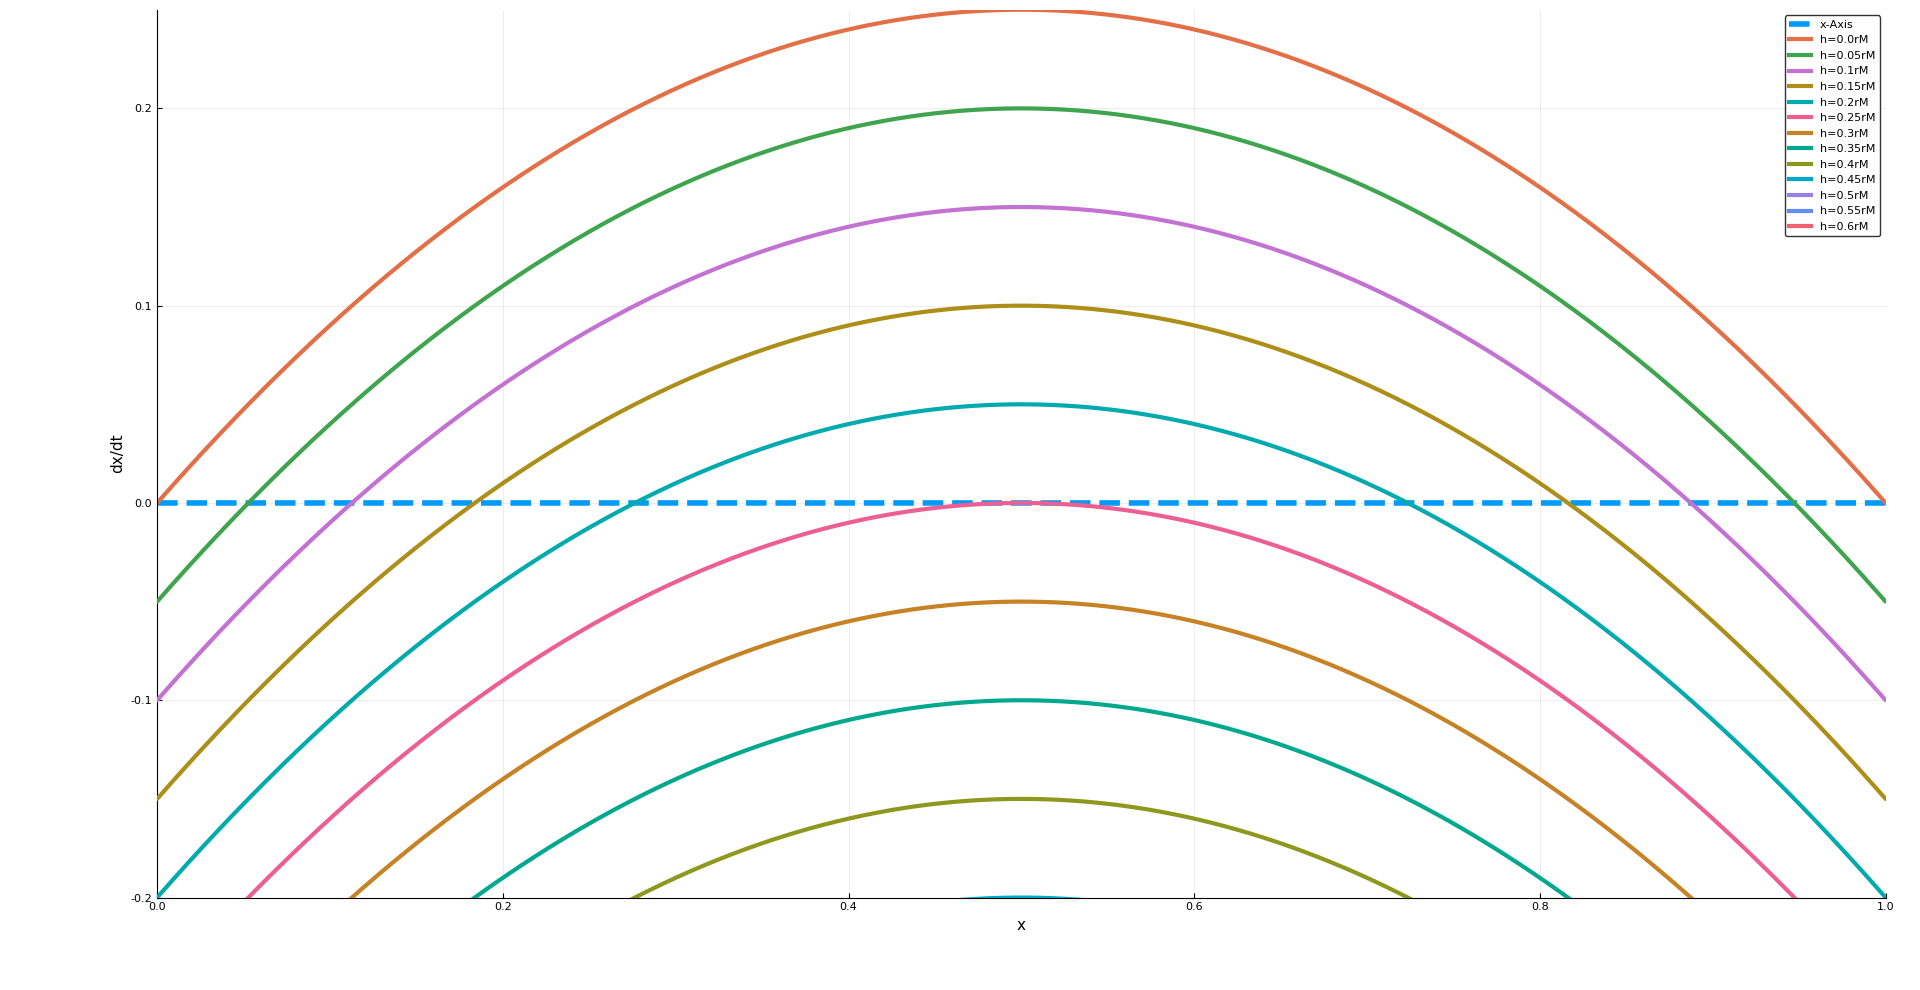
\includegraphics[width=0.8\textwidth]{CriticalPoints.png}
	\caption{Figure representing $\dev{x}{t}$ with different harvesting rates.}
	\label{fig: CriticalPoints}
\end{figure}
\begin{figure}
		\centering
		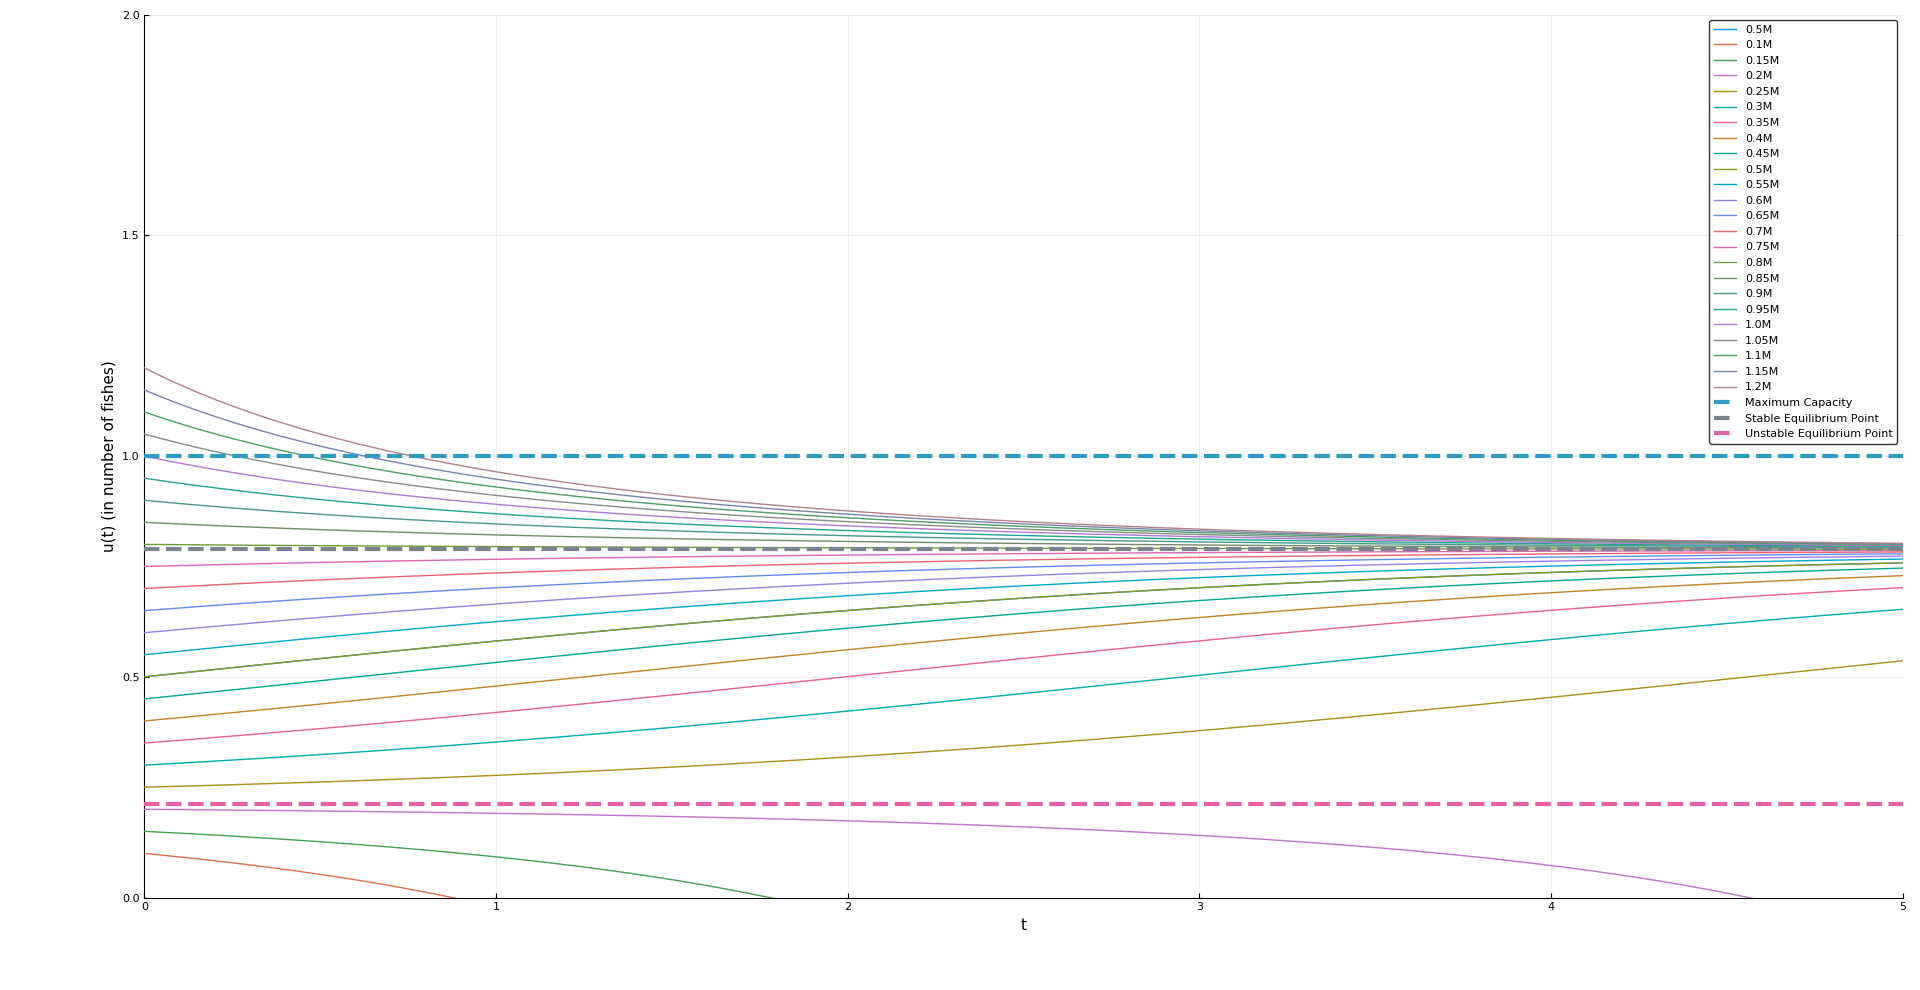
\includegraphics[width=0.8\textwidth]{SustainableConstant.png}
		\caption{Constant harvest rate $u<\frac{rM}{4}$.}
		\label{fig: SustainableConstantHarvest}
\end{figure}
\begin{figure}
	\centering
	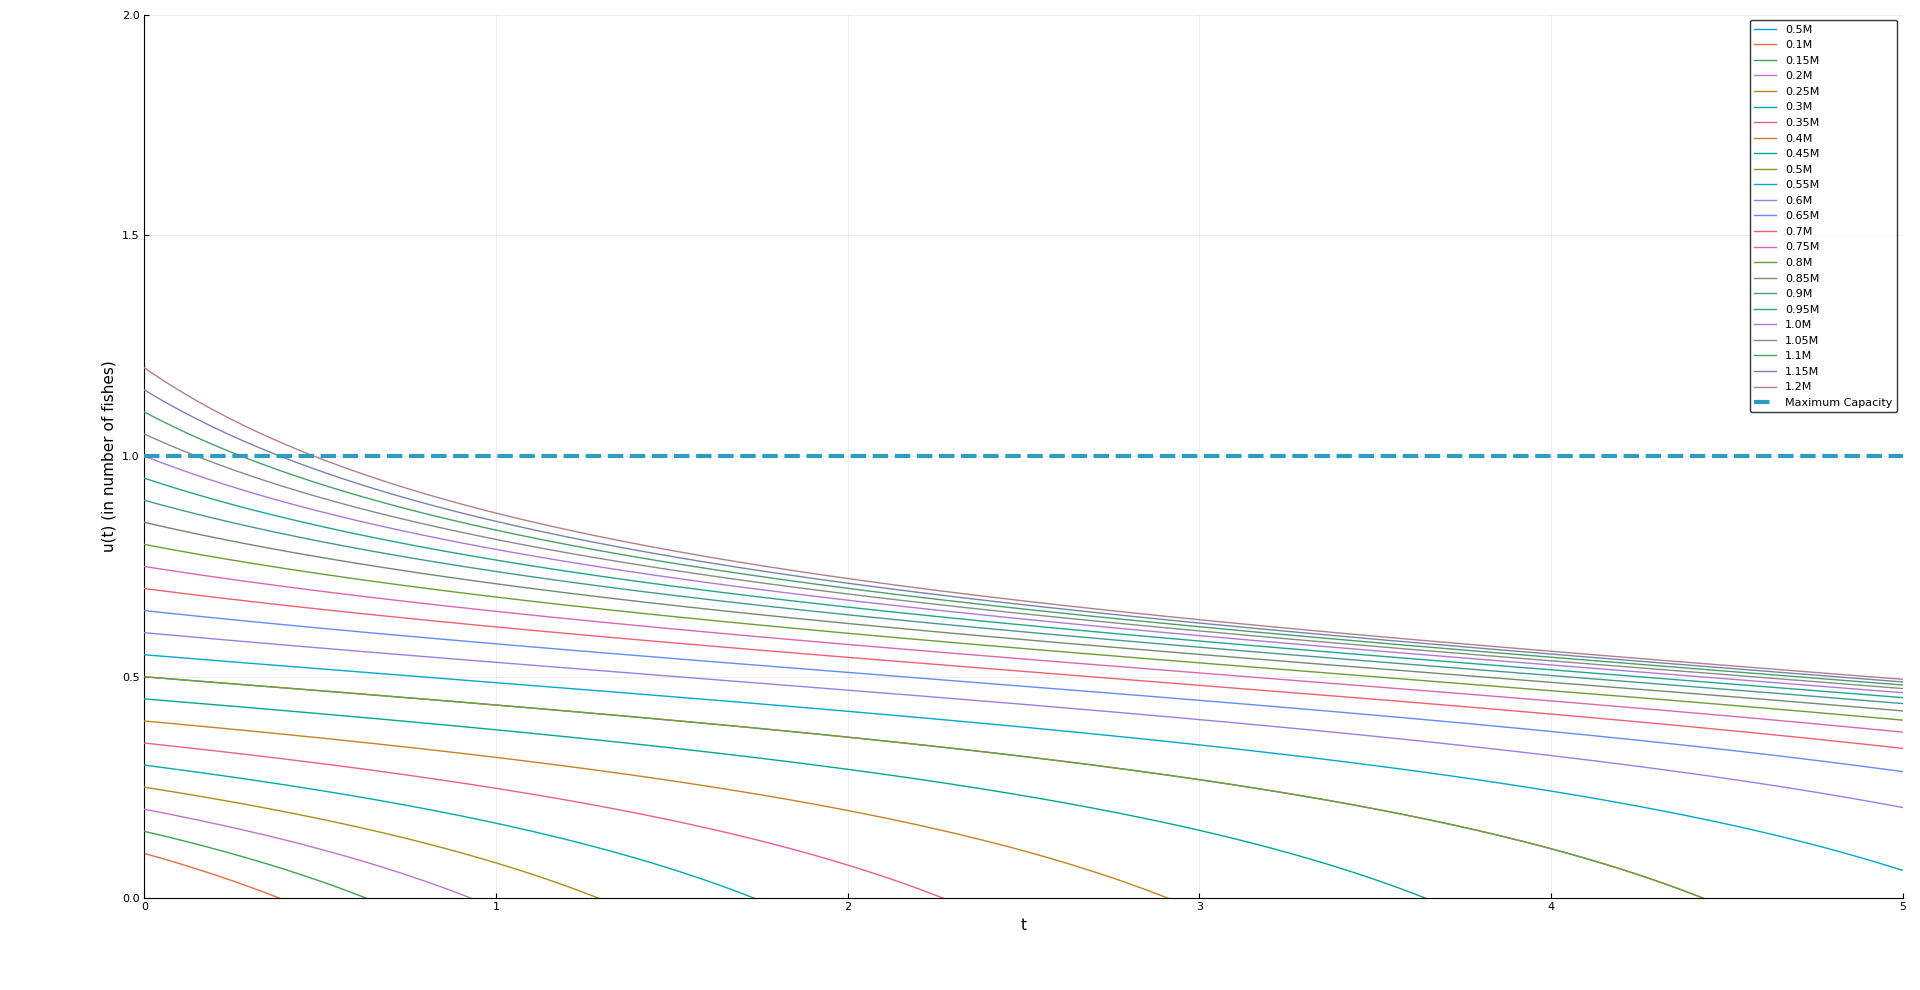
\includegraphics[width=0.8\textwidth]{OverExploitConstant.png}
	\caption{Constant harvest rate $u>\frac{rM}{4}$.}
	\label{fig: OverExploitConstantHarvest}
\end{figure}

\begin{figure}
	\centering
	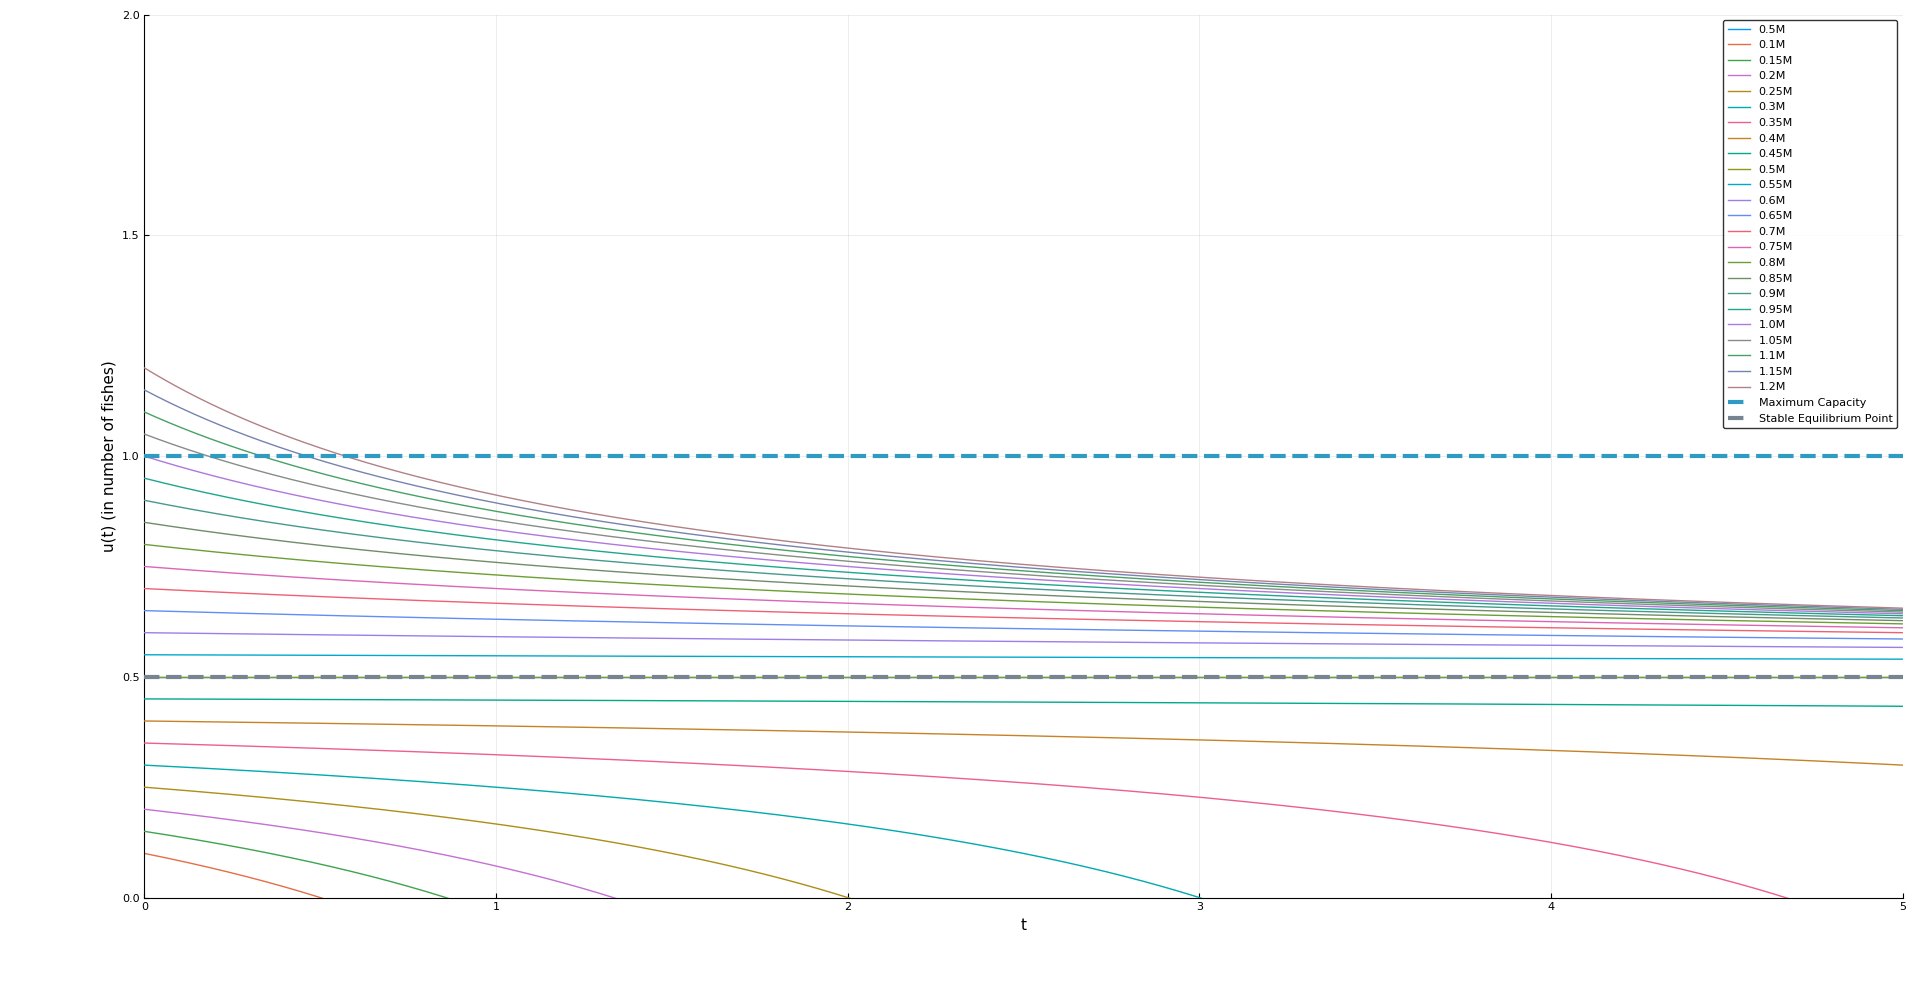
\includegraphics[width=0.8\textwidth]{CriticalExploitConstant.png}
	\caption{Constant harvest rate $u=\frac{rM}{4}$.}
	\label{fig: CriticalExploitConstantHarvest}
\end{figure}


	\section{Closed Loop Strategies.}
	\label{sec: ClosedLoop}
		\graphicspath{{FishingStrategies/ClosedLoop/}}
		\begin{equation}
\dev{x}{t}=rx\left(1-\frac{x}{M}\right)-u \label{eq: ConstantHarvest}
\end{equation}
We introduce the following variable in order to simply calculations,
\begin{equation}
\beta=\frac{uM}{r}
\end{equation}
Solving the differential equation,
\begin{align*}
	\frac{\diff{x}}{rx\left(1-\frac{x}{M}\right)-u}&=\diff{t} \\
	\int_{x_0}^{x}\frac{\diff{\chi}}{r\chi\left(1-\frac{\chi}{M}\right)-u}&=\int_{0}^{t}\diff{\tau} \\
	\frac{M}{r}\int_{x_0}^{x}\frac{\diff{\chi}}{\chi\left(M-\chi\right)-\frac{Mu}{r}}&=t \\
	-\frac{M}{r}\int_{x_0}^{x}\frac{\diff{\chi}}{\chi^2-M\chi+\beta}&=t \nonumber
	\end{align*}
Finally, we model the above integral as one 
\begin{align}
	-\frac{M}{r}\int_{x_0}^{x}\frac{\diff{\chi}}{\left(\chi-\frac{M}{2}\right)^2-\frac{M^2}{4}+\beta}&=t
\end{align}
Consider $\alpha$ as follows,
\begin{equation}
	\alpha = \beta - \frac{M^2}{4} = rM\left(u-\frac{rM}{4}\right)
\end{equation}
We see that the sign of $\alpha$ determines the nature of the solutions. Then, if $u>rM/4$ implies $\alpha>0$,
\begin{align*}
\int_{x_0}^{x}\frac{\diff{\chi}}{\left(\chi-\frac{M}{2}\right)^2+\alpha}&=-\frac{r}{M}t \\
\frac{1}{\sqrt{\beta-\frac{M^2}{4}}}\left(\arctan\left(\frac{x-M/2}{\sqrt{\beta-M^2/4}}\right)-\arctan\left(\frac{x_0-M/2}{\sqrt{\beta-M^2/4}}\right)\right)&=-\frac{r}{M}t \\
\end{align*}
Therefore, for $\alpha > 0$ the population behaves as follows, 
\begin{align}
	x(t)=\frac{M}{2}+\sqrt{\beta-\frac{M^2}{4}} \tan \left(\arctan\left(\frac{x_0-M/2}{\sqrt{\beta-M^2/4}}\right)-\frac{r\sqrt{\beta-M^2/4}}{M}t\right) \label{eq: ConstantHarvest OverExploit}
\end{align}

Equation \ref{eq: ConstantHarvest OverExploit} show us that for some $t^*$, $x(t^*)=0$,independently of the initial condition $x_0$, since the argument inside the $\tan$ is monotone decreasing in $t$. 

If $u<rM/4$ implies $-\alpha>0$,
\begin{align*}
	\int_{x_0}^{x}\frac{\diff{\chi}}{\left(\chi-\frac{M}{2}\right)^2-(-\alpha)} &=-\frac{r}{M}t
\end{align*}
Considering the zeros of the denominator, $\lambda$ and $\overleftarrow{\lambda}$, 
\begin{equation}
	\begin{array}{cc}
	\lambda&=\frac{M}{2}+\sqrt{\frac{M^2}{4}-\beta} \\
	\overline{\lambda}&=\frac{M}{2}-\sqrt{\frac{M^2}{4}-\beta} \\
	\end{array}
\end{equation}
We can rewrite our expression as follows, 
\begin{align*}
\int_{x_0}^{x} \left(\frac{1}{\chi - \lambda}-\frac{1}{\chi - \overline{\lambda}}\right)\diff{\chi} &=-\frac{2r\sqrt{M^2/4-\beta}}{M}t \\
	\ln\abs{\frac{x - \lambda}{x - \overline{\lambda}}}&=\ln\abs{\frac{x_0- \lambda}{x_0 - \overline{\lambda}}}-\frac{2r\sqrt{M^2/4-\beta}}{M}t
\end{align*}
For simplifying calculations, we write, $\gamma=\frac{2r\sqrt{M^2/4-\beta}}{M}$. And we obtain as result,
\begin{align}
\frac{x - \lambda}{x - \overline{\lambda}} &=\frac{x_0- \lambda}{x_0- \overline{\lambda}}\mathrm e^{-\gamma t} \\
x-\lambda &=\left(x-\overline{\lambda}\right)\left(\frac{x_0- \lambda}{x_0- \overline{\lambda}}\right)\mathrm e^{-\gamma t}
\end{align}

For the sake of simplicity, consider $\xi=\frac{x_0-\lambda}{x_0-\overline{\lambda}}\mathrm{e}^{-\gamma t}$. Therefore,
\begin{align*}
	x\left(1-\xi\right)&=\lambda-\overline{\lambda}\xi\\
	x&=\frac{\lambda-\overline{\lambda}\xi}{1-\xi} \\	
	x&=\frac{\frac{M}{2}+\sqrt{\frac{M^2}{4}-\beta}-\left(\frac{M}{2}-\sqrt{\frac{M^2}{4}-\beta}\right)\xi}{1-\xi}\\
	x&=\frac{\frac{M}{2}+\sqrt{\frac{M^2}{4}-\beta}-\left(\frac{M}{2}-\sqrt{\frac{M^2}{4}-\beta}\right)\xi}{1-\xi}\\
	x&=\frac{\frac{M}{2}\left(1-\xi\right)+\sqrt{\frac{M^2}{4}-\beta}\left(1+\xi\right)}{1-\xi}\\
	x&=\frac{M}{2}+\sqrt{\frac{M^2}{4}-\beta}\frac{1+\xi}{1-\xi}
\end{align*}
Hence, for $-\alpha>0$, we have the following result,
\begin{align}
	x(t)&=\frac{M}{2}+\left(\sqrt{\frac{M^2}{4}-\beta}\right)\frac{\left(x_0-M/2\right)\left(1+\mathrm e^{-\gamma t}\right)-\sqrt{M^2/4-\beta}\left(1-\mathrm{e}^{-\gamma t}\right)}{\left(x_0-M/2\right)\left(1-\mathrm e^{-\gamma t}\right)+\sqrt{M^2/4-\beta}\left(1+\mathrm{e}^{-\gamma t}\right)} \label{eq: Time Expression for Harvest}
\end{align}

If $u=\frac{rM}{4}$, we solve equation \ref{eq: ConstantHarvest} as follows,
\begin{align}
-\frac{M}{r}\int_{x_0}^{x}\frac{d\chi}{\left(\chi-\frac{M}{2}\right)^2}&=t\\
\int_{x_0}^{x}\frac{d\chi}{\left(\chi-\frac{M}{2}\right)^2}&=-\frac{rt}{M}\\
\frac{1}{x-\frac{M}{2}}&=\frac{1}{x_0-\frac{M}{2}}-\frac{rt}{M}\\
\frac{1}{x-\frac{M}{2}}&=\frac{M-\left(x_0-\frac{M}{2}\right)rt}{M\left(x_0-\frac{M}{2}\right)} \\
x&=\frac{M}{2}+\frac{M\left(x_0-\frac{M}{2}\right)}{M-\left(x_0-\frac{M}{2}\right)rt} 
\end{align}

The results above stated can be explained directly from the equation \ref{eq: ConstantHarvest}, as we see in the graph \ref{fig: CriticalPoints},  $F(x,t)$ is a paraboloid, with its maximum at $F(x^*=M/2,t)=rM^2/4$.

When $u=0$, we have the regular logistic equation with critical points $x_{c_1}=0$ and $x_{c_2}=M$. With $x_{c_2}$ being an stable fixed point and $x_{c_1}$ an unstable fixed point. In general, these are the solutions to the equation $F(x,t)-u=0$,
\begin{equation}
x_{c_{2,1}}=\frac{M}{2}\pm \sqrt{\frac{M^2}{4}-u\frac{M}{r}}
\end{equation}

We observe that the critical points $x_c$, such that $\dev{x_c}{t}=F(x_c, t)-u=0$ are getting closer to each other, as $u$ is increasing; when $u=\frac{rM}{4}$ we only have one critical unstable point. That behaves as an attractor when $x_0\geq\frac{M}{2}$. But when $x_0<\frac{M}{2}$ the population strictly decreases. For $u> \frac{rM}{4}$, the population $x(t)$ has no real critical points and the derivative $\dev{x}{t}$ is always negative, implying, that we will lead always the population to extinction, extracting constantly at a rate greater than $\frac{rM}{4}$.

\begin{figure}[H]
	\centering
	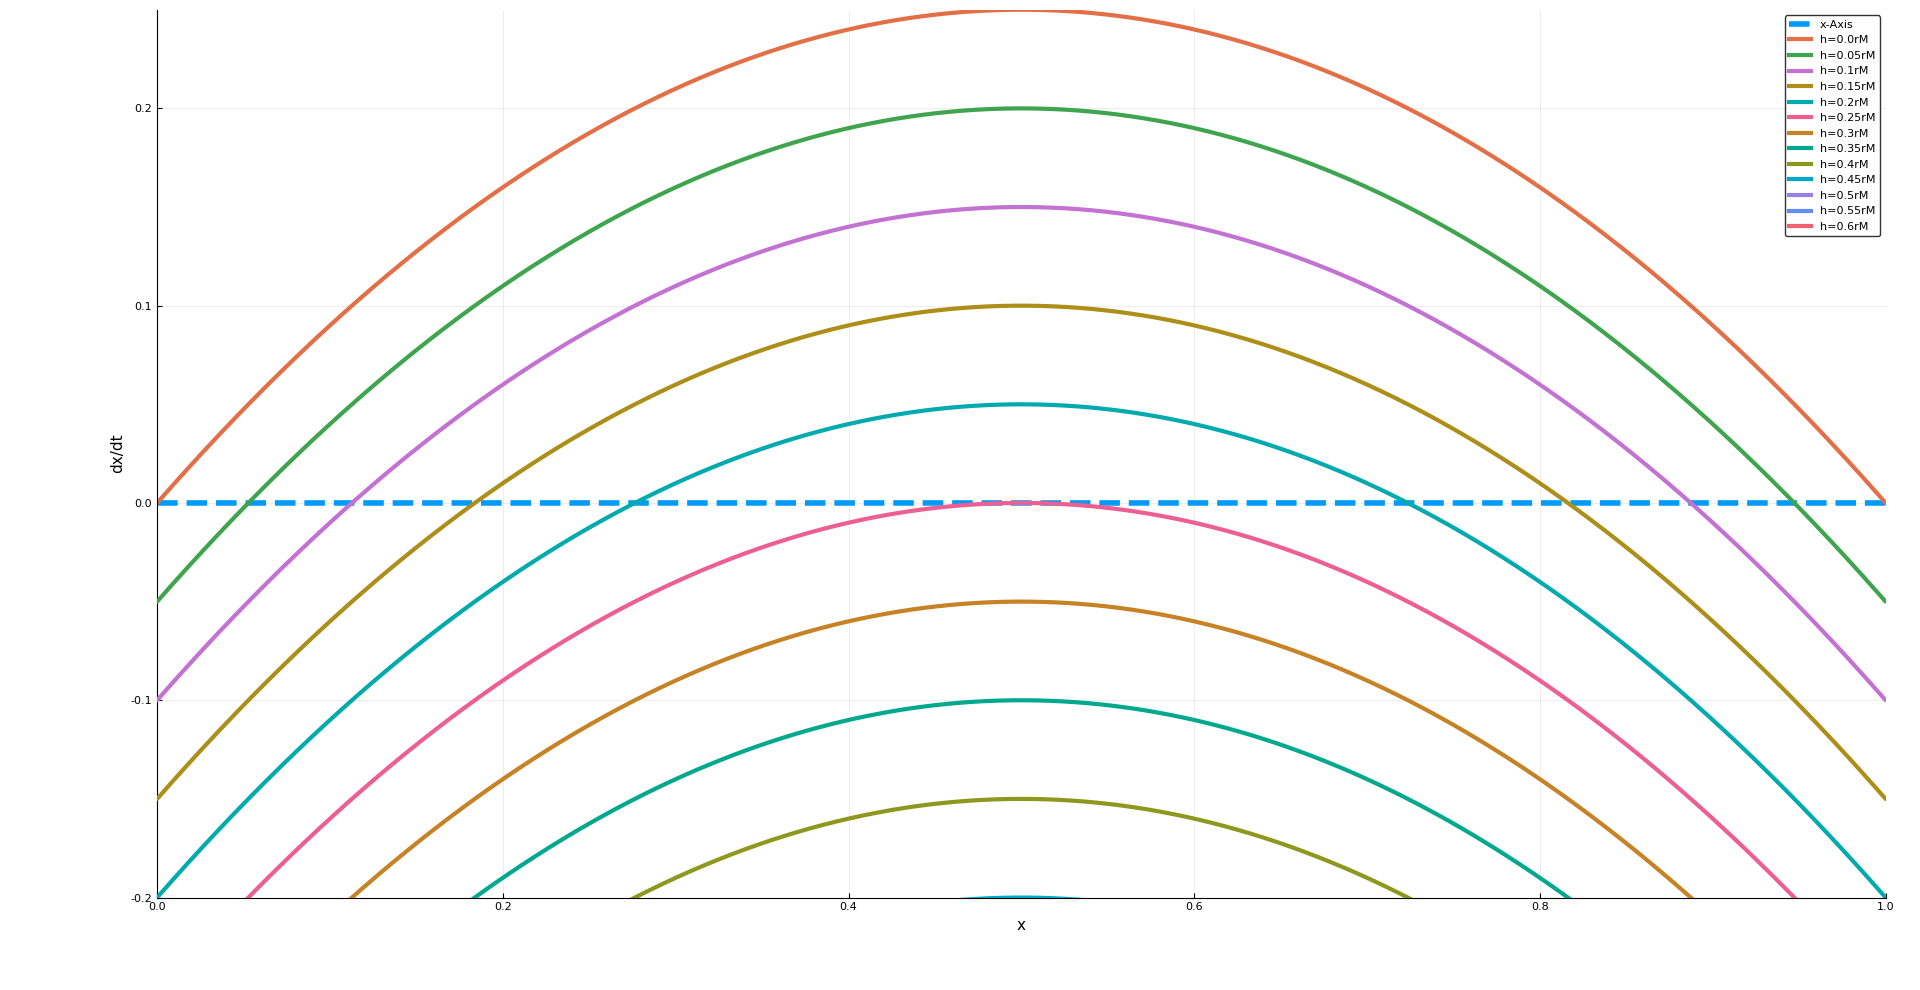
\includegraphics[width=0.8\textwidth]{CriticalPoints.png}
	\caption{Figure representing $\dev{x}{t}$ with different harvesting rates.}
	\label{fig: CriticalPoints}
\end{figure}
\begin{figure}
		\centering
		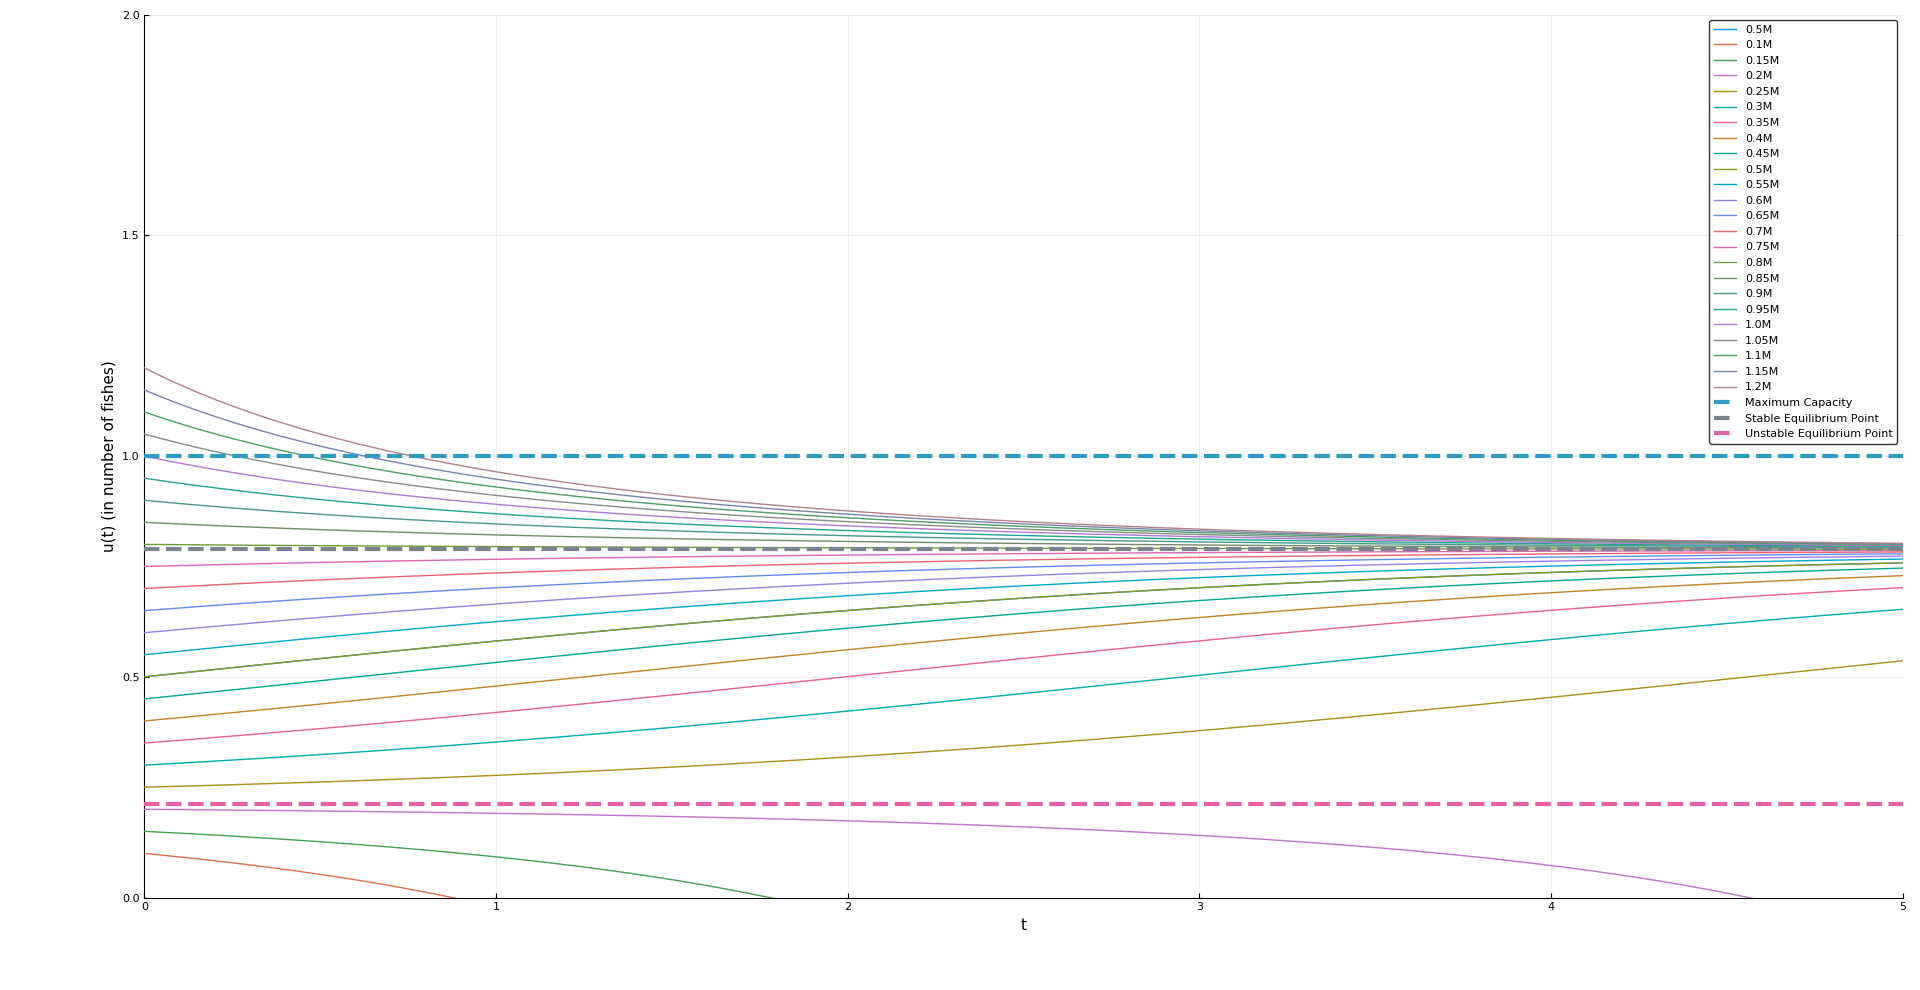
\includegraphics[width=0.8\textwidth]{SustainableConstant.png}
		\caption{Constant harvest rate $u<\frac{rM}{4}$.}
		\label{fig: SustainableConstantHarvest}
\end{figure}
\begin{figure}
	\centering
	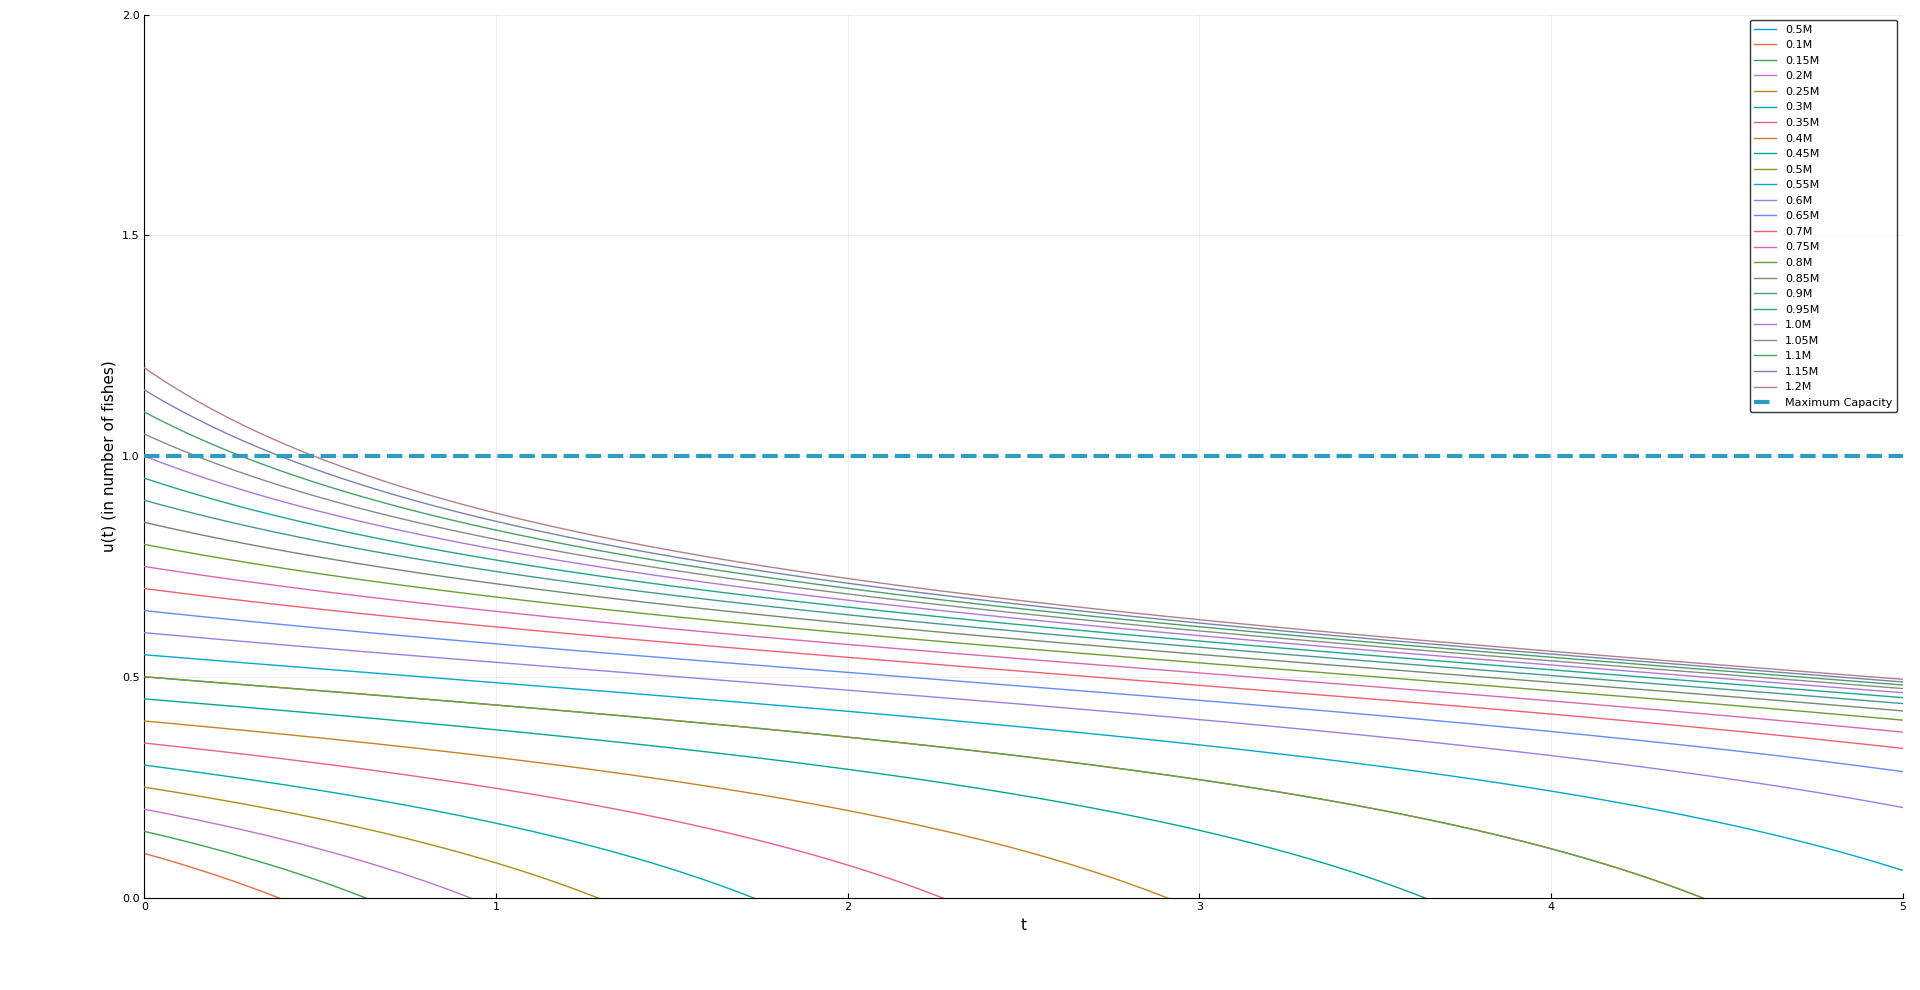
\includegraphics[width=0.8\textwidth]{OverExploitConstant.png}
	\caption{Constant harvest rate $u>\frac{rM}{4}$.}
	\label{fig: OverExploitConstantHarvest}
\end{figure}

\begin{figure}
	\centering
	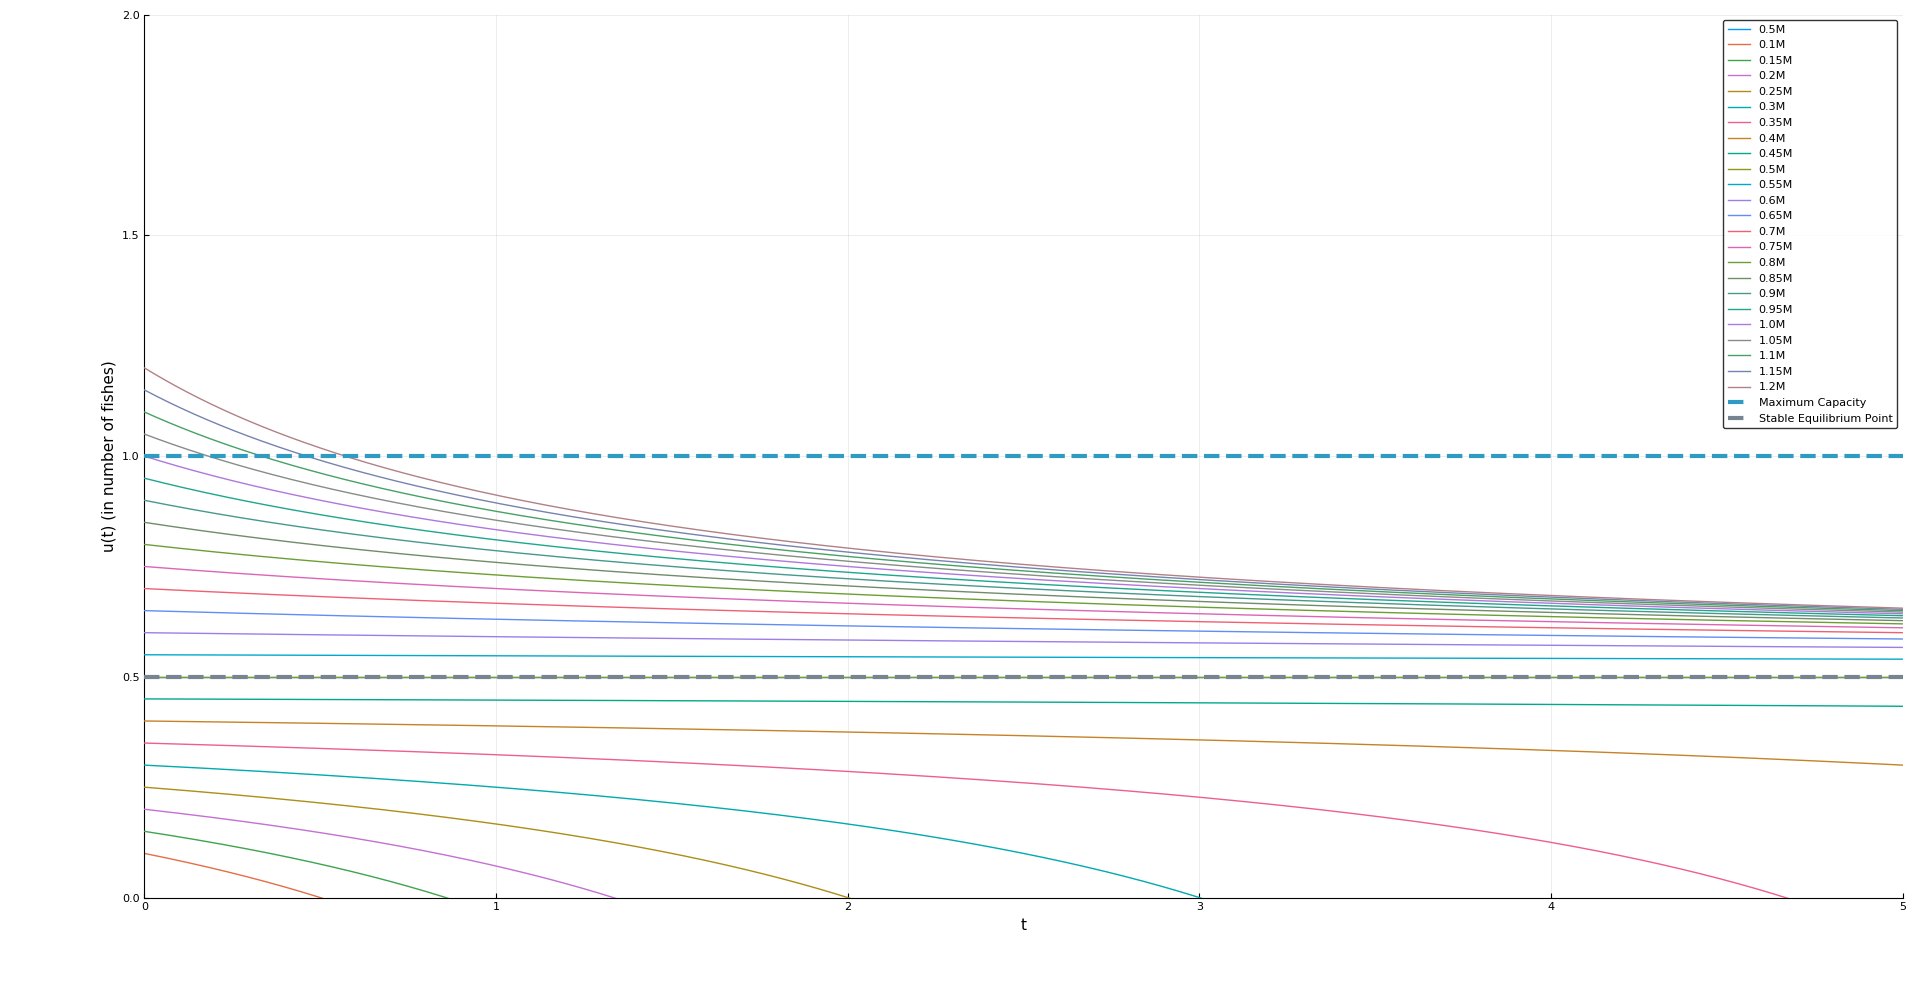
\includegraphics[width=0.8\textwidth]{CriticalExploitConstant.png}
	\caption{Constant harvest rate $u=\frac{rM}{4}$.}
	\label{fig: CriticalExploitConstantHarvest}
\end{figure}


		\subsection{Constant Proportional Harvesting.}
		\graphicspath{{FishingStrategies/ClosedLoop/ConstantProportional/}}
		\begin{equation}
\dev{x}{t}=rx\left(1-\frac{x}{M}\right)-u \label{eq: ConstantHarvest}
\end{equation}
We introduce the following variable in order to simply calculations,
\begin{equation}
\beta=\frac{uM}{r}
\end{equation}
Solving the differential equation,
\begin{align*}
	\frac{\diff{x}}{rx\left(1-\frac{x}{M}\right)-u}&=\diff{t} \\
	\int_{x_0}^{x}\frac{\diff{\chi}}{r\chi\left(1-\frac{\chi}{M}\right)-u}&=\int_{0}^{t}\diff{\tau} \\
	\frac{M}{r}\int_{x_0}^{x}\frac{\diff{\chi}}{\chi\left(M-\chi\right)-\frac{Mu}{r}}&=t \\
	-\frac{M}{r}\int_{x_0}^{x}\frac{\diff{\chi}}{\chi^2-M\chi+\beta}&=t \nonumber
	\end{align*}
Finally, we model the above integral as one 
\begin{align}
	-\frac{M}{r}\int_{x_0}^{x}\frac{\diff{\chi}}{\left(\chi-\frac{M}{2}\right)^2-\frac{M^2}{4}+\beta}&=t
\end{align}
Consider $\alpha$ as follows,
\begin{equation}
	\alpha = \beta - \frac{M^2}{4} = rM\left(u-\frac{rM}{4}\right)
\end{equation}
We see that the sign of $\alpha$ determines the nature of the solutions. Then, if $u>rM/4$ implies $\alpha>0$,
\begin{align*}
\int_{x_0}^{x}\frac{\diff{\chi}}{\left(\chi-\frac{M}{2}\right)^2+\alpha}&=-\frac{r}{M}t \\
\frac{1}{\sqrt{\beta-\frac{M^2}{4}}}\left(\arctan\left(\frac{x-M/2}{\sqrt{\beta-M^2/4}}\right)-\arctan\left(\frac{x_0-M/2}{\sqrt{\beta-M^2/4}}\right)\right)&=-\frac{r}{M}t \\
\end{align*}
Therefore, for $\alpha > 0$ the population behaves as follows, 
\begin{align}
	x(t)=\frac{M}{2}+\sqrt{\beta-\frac{M^2}{4}} \tan \left(\arctan\left(\frac{x_0-M/2}{\sqrt{\beta-M^2/4}}\right)-\frac{r\sqrt{\beta-M^2/4}}{M}t\right) \label{eq: ConstantHarvest OverExploit}
\end{align}

Equation \ref{eq: ConstantHarvest OverExploit} show us that for some $t^*$, $x(t^*)=0$,independently of the initial condition $x_0$, since the argument inside the $\tan$ is monotone decreasing in $t$. 

If $u<rM/4$ implies $-\alpha>0$,
\begin{align*}
	\int_{x_0}^{x}\frac{\diff{\chi}}{\left(\chi-\frac{M}{2}\right)^2-(-\alpha)} &=-\frac{r}{M}t
\end{align*}
Considering the zeros of the denominator, $\lambda$ and $\overleftarrow{\lambda}$, 
\begin{equation}
	\begin{array}{cc}
	\lambda&=\frac{M}{2}+\sqrt{\frac{M^2}{4}-\beta} \\
	\overline{\lambda}&=\frac{M}{2}-\sqrt{\frac{M^2}{4}-\beta} \\
	\end{array}
\end{equation}
We can rewrite our expression as follows, 
\begin{align*}
\int_{x_0}^{x} \left(\frac{1}{\chi - \lambda}-\frac{1}{\chi - \overline{\lambda}}\right)\diff{\chi} &=-\frac{2r\sqrt{M^2/4-\beta}}{M}t \\
	\ln\abs{\frac{x - \lambda}{x - \overline{\lambda}}}&=\ln\abs{\frac{x_0- \lambda}{x_0 - \overline{\lambda}}}-\frac{2r\sqrt{M^2/4-\beta}}{M}t
\end{align*}
For simplifying calculations, we write, $\gamma=\frac{2r\sqrt{M^2/4-\beta}}{M}$. And we obtain as result,
\begin{align}
\frac{x - \lambda}{x - \overline{\lambda}} &=\frac{x_0- \lambda}{x_0- \overline{\lambda}}\mathrm e^{-\gamma t} \\
x-\lambda &=\left(x-\overline{\lambda}\right)\left(\frac{x_0- \lambda}{x_0- \overline{\lambda}}\right)\mathrm e^{-\gamma t}
\end{align}

For the sake of simplicity, consider $\xi=\frac{x_0-\lambda}{x_0-\overline{\lambda}}\mathrm{e}^{-\gamma t}$. Therefore,
\begin{align*}
	x\left(1-\xi\right)&=\lambda-\overline{\lambda}\xi\\
	x&=\frac{\lambda-\overline{\lambda}\xi}{1-\xi} \\	
	x&=\frac{\frac{M}{2}+\sqrt{\frac{M^2}{4}-\beta}-\left(\frac{M}{2}-\sqrt{\frac{M^2}{4}-\beta}\right)\xi}{1-\xi}\\
	x&=\frac{\frac{M}{2}+\sqrt{\frac{M^2}{4}-\beta}-\left(\frac{M}{2}-\sqrt{\frac{M^2}{4}-\beta}\right)\xi}{1-\xi}\\
	x&=\frac{\frac{M}{2}\left(1-\xi\right)+\sqrt{\frac{M^2}{4}-\beta}\left(1+\xi\right)}{1-\xi}\\
	x&=\frac{M}{2}+\sqrt{\frac{M^2}{4}-\beta}\frac{1+\xi}{1-\xi}
\end{align*}
Hence, for $-\alpha>0$, we have the following result,
\begin{align}
	x(t)&=\frac{M}{2}+\left(\sqrt{\frac{M^2}{4}-\beta}\right)\frac{\left(x_0-M/2\right)\left(1+\mathrm e^{-\gamma t}\right)-\sqrt{M^2/4-\beta}\left(1-\mathrm{e}^{-\gamma t}\right)}{\left(x_0-M/2\right)\left(1-\mathrm e^{-\gamma t}\right)+\sqrt{M^2/4-\beta}\left(1+\mathrm{e}^{-\gamma t}\right)} \label{eq: Time Expression for Harvest}
\end{align}

If $u=\frac{rM}{4}$, we solve equation \ref{eq: ConstantHarvest} as follows,
\begin{align}
-\frac{M}{r}\int_{x_0}^{x}\frac{d\chi}{\left(\chi-\frac{M}{2}\right)^2}&=t\\
\int_{x_0}^{x}\frac{d\chi}{\left(\chi-\frac{M}{2}\right)^2}&=-\frac{rt}{M}\\
\frac{1}{x-\frac{M}{2}}&=\frac{1}{x_0-\frac{M}{2}}-\frac{rt}{M}\\
\frac{1}{x-\frac{M}{2}}&=\frac{M-\left(x_0-\frac{M}{2}\right)rt}{M\left(x_0-\frac{M}{2}\right)} \\
x&=\frac{M}{2}+\frac{M\left(x_0-\frac{M}{2}\right)}{M-\left(x_0-\frac{M}{2}\right)rt} 
\end{align}

The results above stated can be explained directly from the equation \ref{eq: ConstantHarvest}, as we see in the graph \ref{fig: CriticalPoints},  $F(x,t)$ is a paraboloid, with its maximum at $F(x^*=M/2,t)=rM^2/4$.

When $u=0$, we have the regular logistic equation with critical points $x_{c_1}=0$ and $x_{c_2}=M$. With $x_{c_2}$ being an stable fixed point and $x_{c_1}$ an unstable fixed point. In general, these are the solutions to the equation $F(x,t)-u=0$,
\begin{equation}
x_{c_{2,1}}=\frac{M}{2}\pm \sqrt{\frac{M^2}{4}-u\frac{M}{r}}
\end{equation}

We observe that the critical points $x_c$, such that $\dev{x_c}{t}=F(x_c, t)-u=0$ are getting closer to each other, as $u$ is increasing; when $u=\frac{rM}{4}$ we only have one critical unstable point. That behaves as an attractor when $x_0\geq\frac{M}{2}$. But when $x_0<\frac{M}{2}$ the population strictly decreases. For $u> \frac{rM}{4}$, the population $x(t)$ has no real critical points and the derivative $\dev{x}{t}$ is always negative, implying, that we will lead always the population to extinction, extracting constantly at a rate greater than $\frac{rM}{4}$.

\begin{figure}[H]
	\centering
	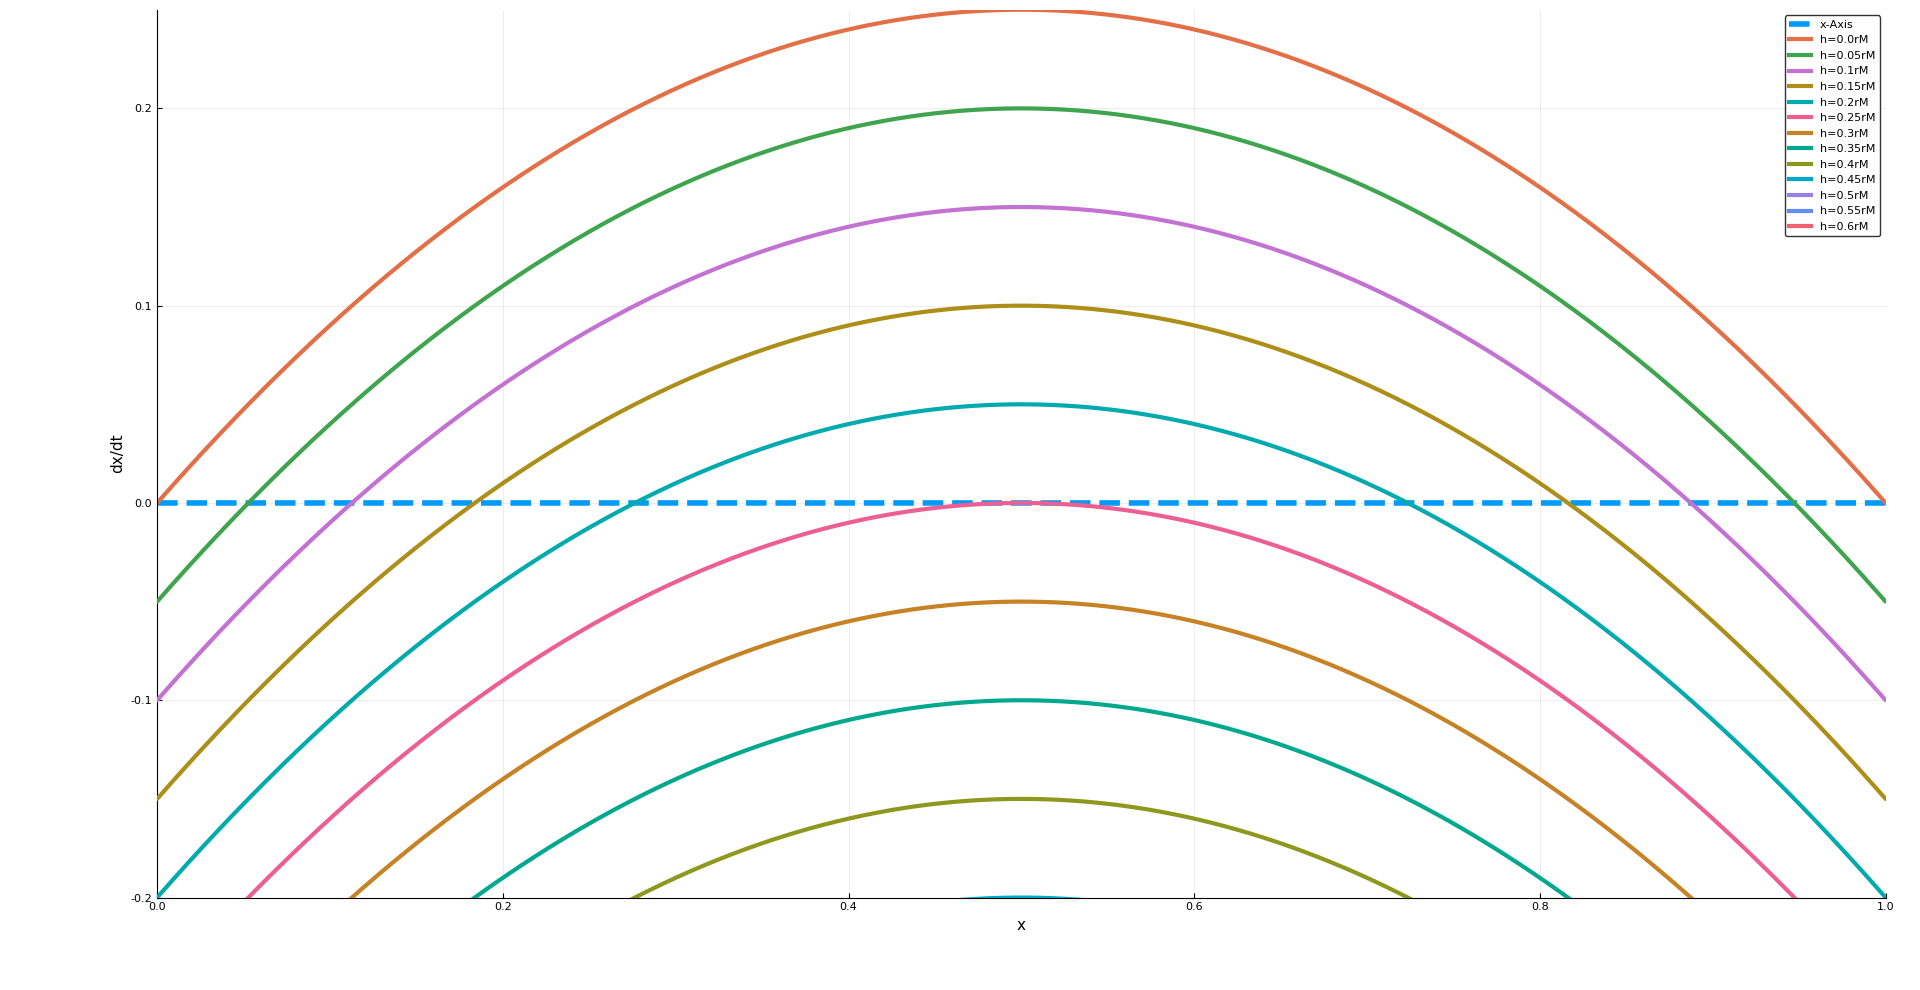
\includegraphics[width=0.8\textwidth]{CriticalPoints.png}
	\caption{Figure representing $\dev{x}{t}$ with different harvesting rates.}
	\label{fig: CriticalPoints}
\end{figure}
\begin{figure}
		\centering
		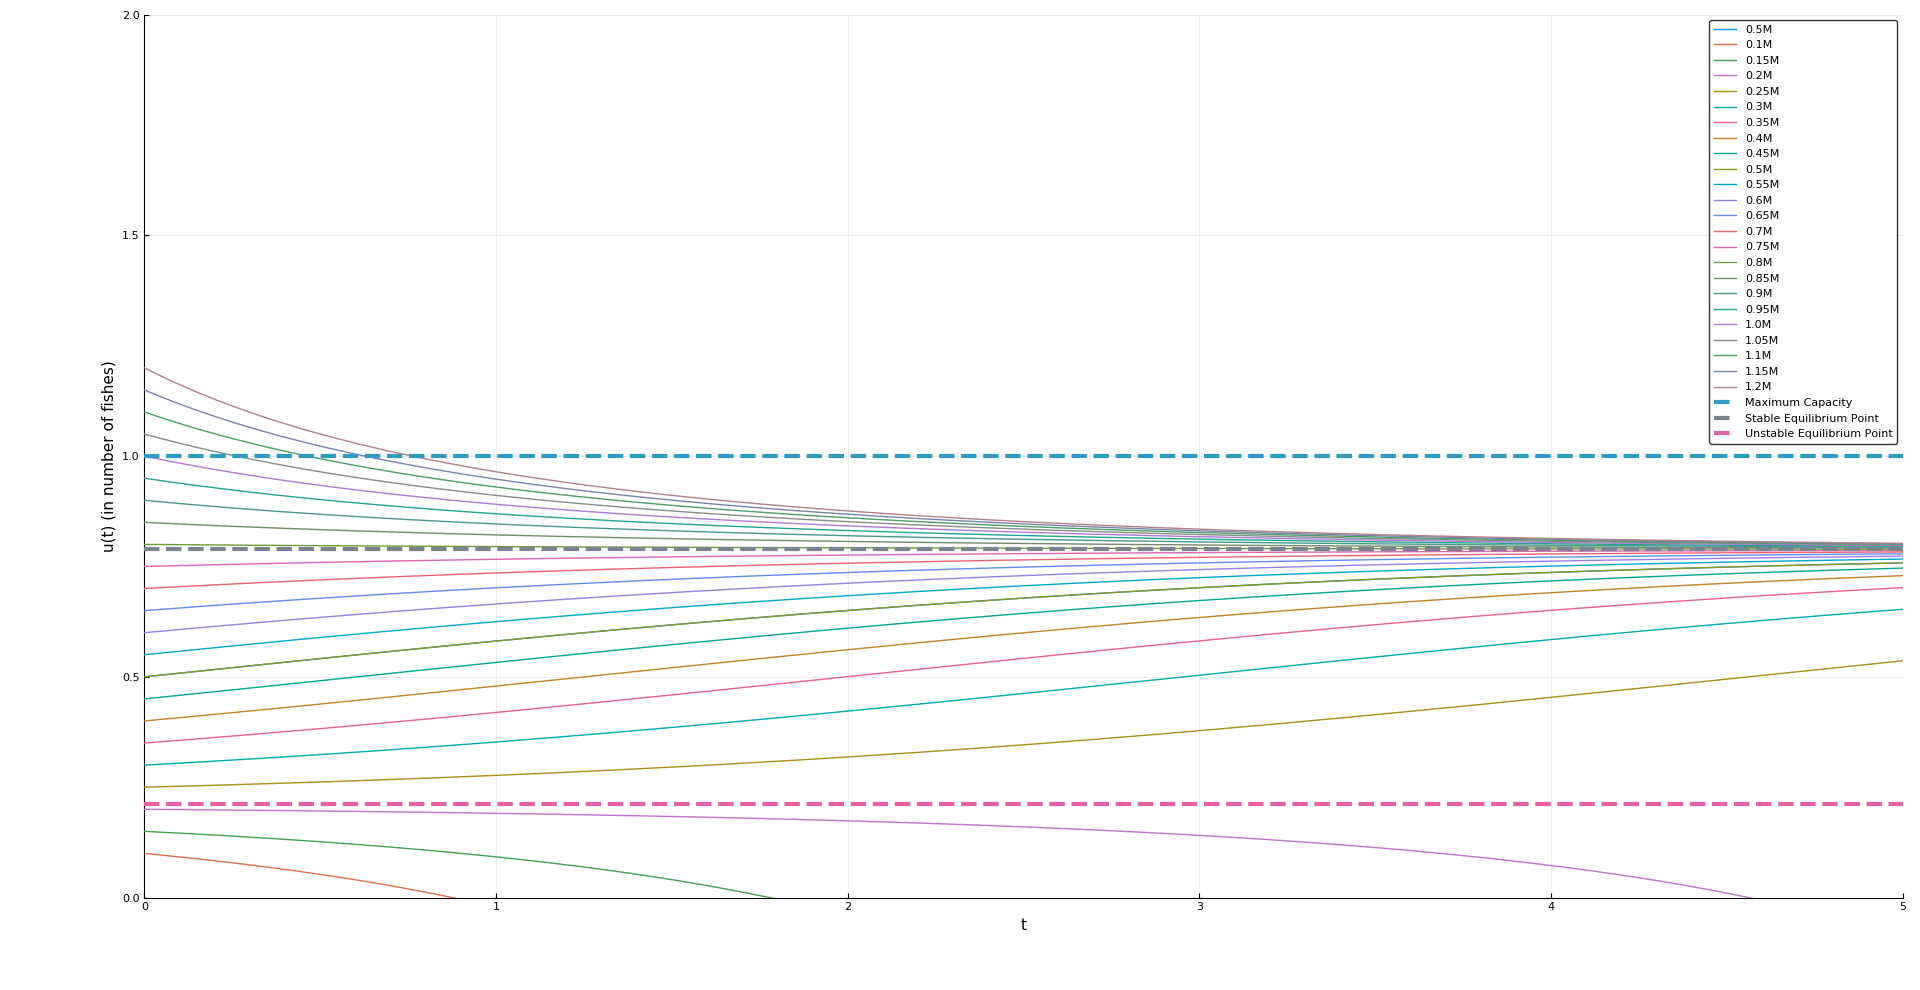
\includegraphics[width=0.8\textwidth]{SustainableConstant.png}
		\caption{Constant harvest rate $u<\frac{rM}{4}$.}
		\label{fig: SustainableConstantHarvest}
\end{figure}
\begin{figure}
	\centering
	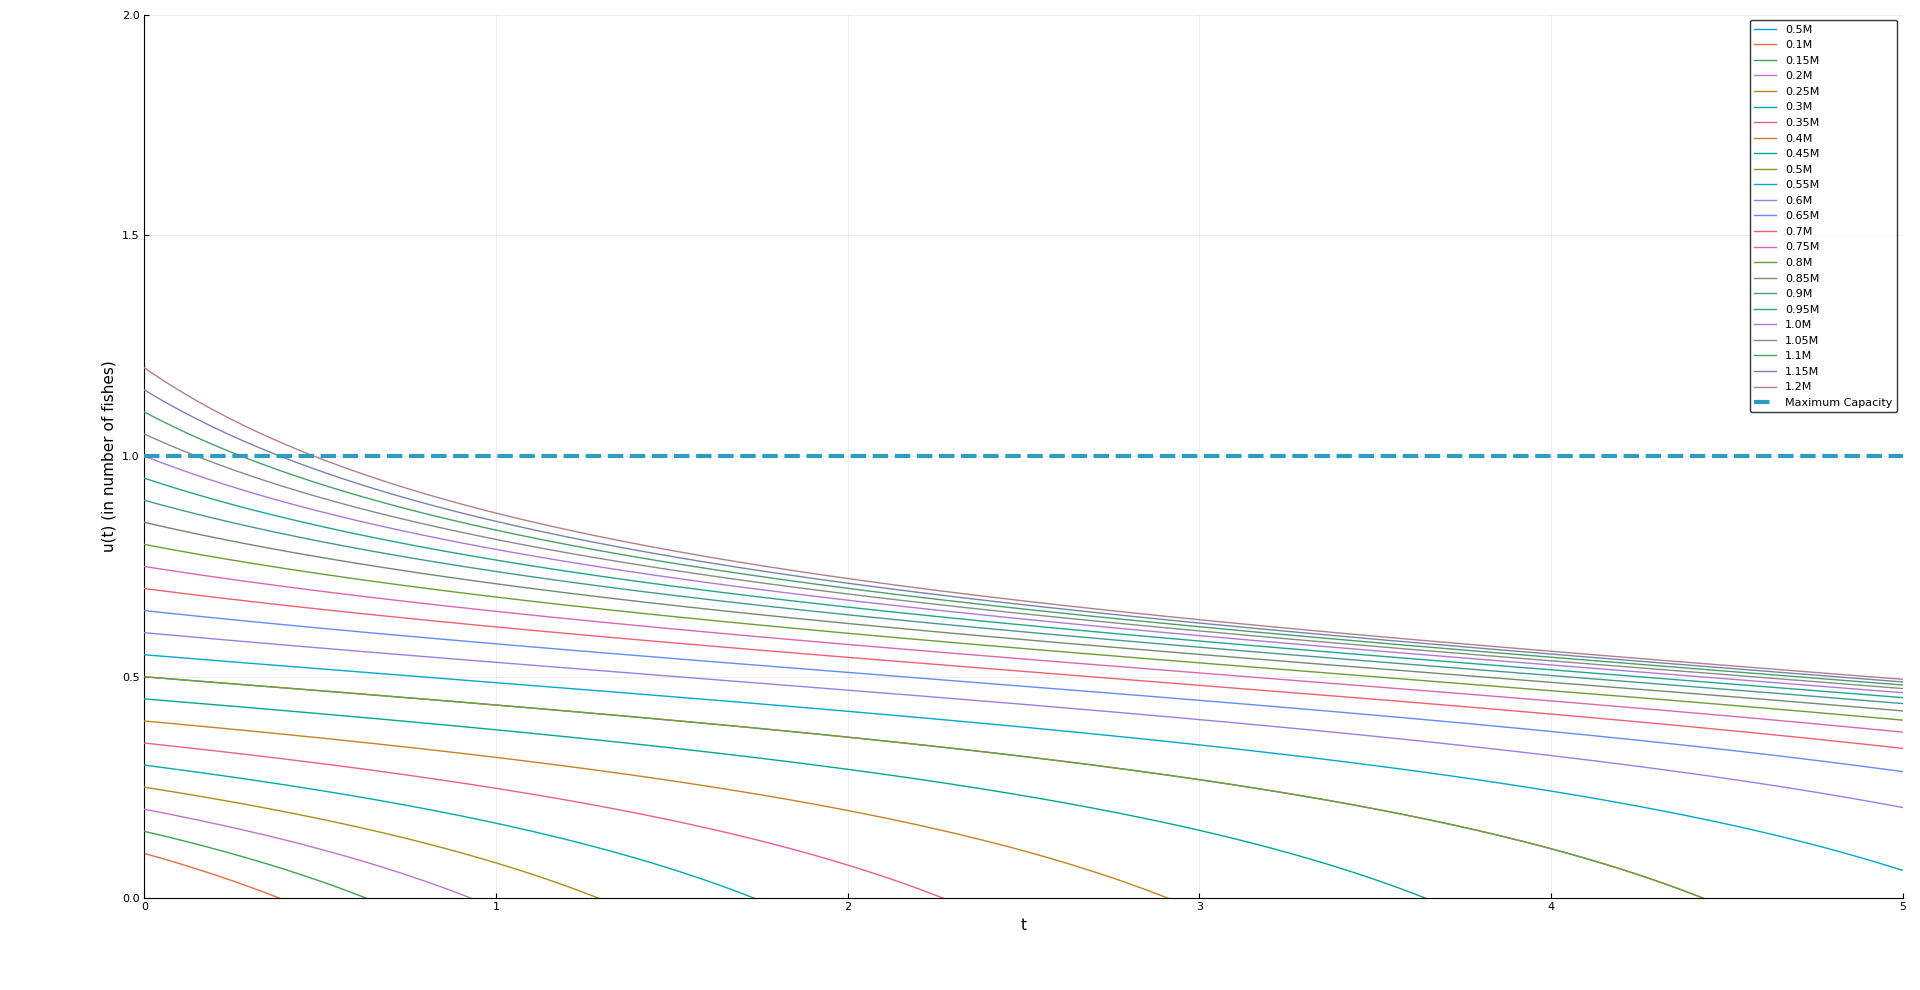
\includegraphics[width=0.8\textwidth]{OverExploitConstant.png}
	\caption{Constant harvest rate $u>\frac{rM}{4}$.}
	\label{fig: OverExploitConstantHarvest}
\end{figure}

\begin{figure}
	\centering
	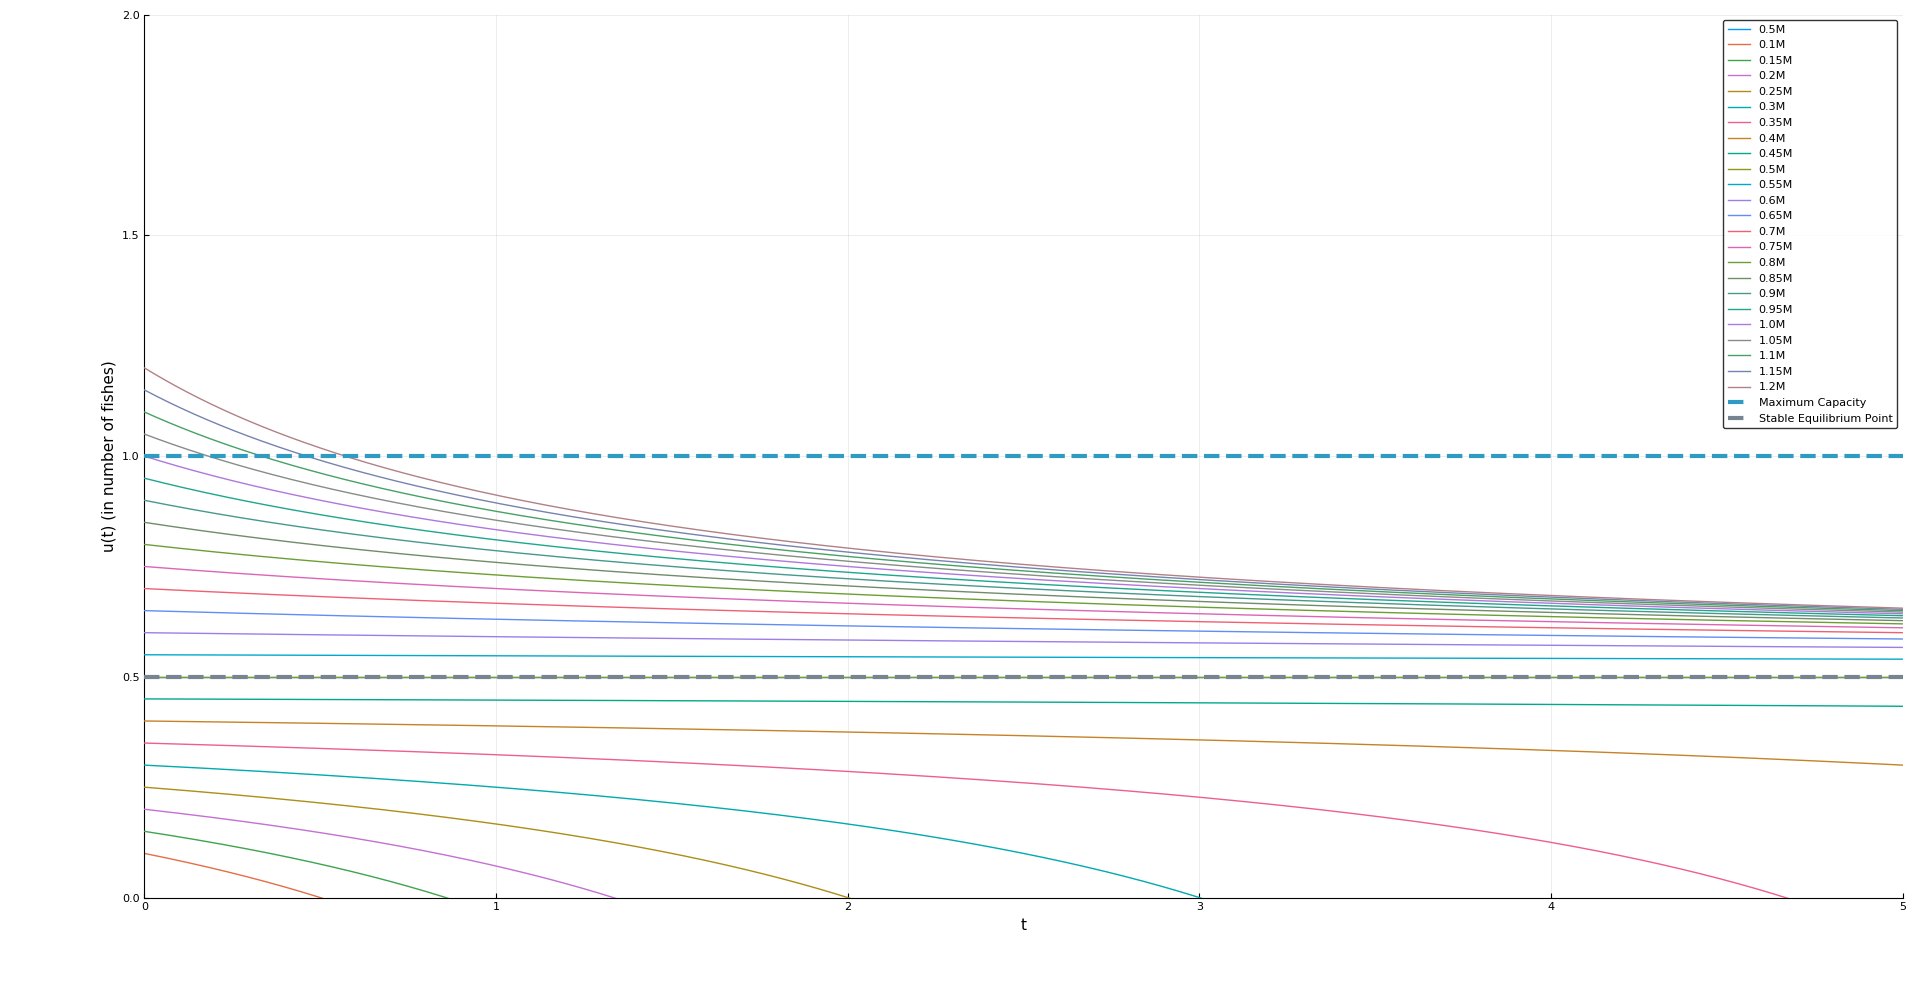
\includegraphics[width=0.8\textwidth]{CriticalExploitConstant.png}
	\caption{Constant harvest rate $u=\frac{rM}{4}$.}
	\label{fig: CriticalExploitConstantHarvest}
\end{figure}


		\subsection{Optimal Proportional Harvesting.}
		\begin{equation}
\dev{x}{t}=rx\left(1-\frac{x}{M}\right)-u \label{eq: ConstantHarvest}
\end{equation}
We introduce the following variable in order to simply calculations,
\begin{equation}
\beta=\frac{uM}{r}
\end{equation}
Solving the differential equation,
\begin{align*}
	\frac{\diff{x}}{rx\left(1-\frac{x}{M}\right)-u}&=\diff{t} \\
	\int_{x_0}^{x}\frac{\diff{\chi}}{r\chi\left(1-\frac{\chi}{M}\right)-u}&=\int_{0}^{t}\diff{\tau} \\
	\frac{M}{r}\int_{x_0}^{x}\frac{\diff{\chi}}{\chi\left(M-\chi\right)-\frac{Mu}{r}}&=t \\
	-\frac{M}{r}\int_{x_0}^{x}\frac{\diff{\chi}}{\chi^2-M\chi+\beta}&=t \nonumber
	\end{align*}
Finally, we model the above integral as one 
\begin{align}
	-\frac{M}{r}\int_{x_0}^{x}\frac{\diff{\chi}}{\left(\chi-\frac{M}{2}\right)^2-\frac{M^2}{4}+\beta}&=t
\end{align}
Consider $\alpha$ as follows,
\begin{equation}
	\alpha = \beta - \frac{M^2}{4} = rM\left(u-\frac{rM}{4}\right)
\end{equation}
We see that the sign of $\alpha$ determines the nature of the solutions. Then, if $u>rM/4$ implies $\alpha>0$,
\begin{align*}
\int_{x_0}^{x}\frac{\diff{\chi}}{\left(\chi-\frac{M}{2}\right)^2+\alpha}&=-\frac{r}{M}t \\
\frac{1}{\sqrt{\beta-\frac{M^2}{4}}}\left(\arctan\left(\frac{x-M/2}{\sqrt{\beta-M^2/4}}\right)-\arctan\left(\frac{x_0-M/2}{\sqrt{\beta-M^2/4}}\right)\right)&=-\frac{r}{M}t \\
\end{align*}
Therefore, for $\alpha > 0$ the population behaves as follows, 
\begin{align}
	x(t)=\frac{M}{2}+\sqrt{\beta-\frac{M^2}{4}} \tan \left(\arctan\left(\frac{x_0-M/2}{\sqrt{\beta-M^2/4}}\right)-\frac{r\sqrt{\beta-M^2/4}}{M}t\right) \label{eq: ConstantHarvest OverExploit}
\end{align}

Equation \ref{eq: ConstantHarvest OverExploit} show us that for some $t^*$, $x(t^*)=0$,independently of the initial condition $x_0$, since the argument inside the $\tan$ is monotone decreasing in $t$. 

If $u<rM/4$ implies $-\alpha>0$,
\begin{align*}
	\int_{x_0}^{x}\frac{\diff{\chi}}{\left(\chi-\frac{M}{2}\right)^2-(-\alpha)} &=-\frac{r}{M}t
\end{align*}
Considering the zeros of the denominator, $\lambda$ and $\overleftarrow{\lambda}$, 
\begin{equation}
	\begin{array}{cc}
	\lambda&=\frac{M}{2}+\sqrt{\frac{M^2}{4}-\beta} \\
	\overline{\lambda}&=\frac{M}{2}-\sqrt{\frac{M^2}{4}-\beta} \\
	\end{array}
\end{equation}
We can rewrite our expression as follows, 
\begin{align*}
\int_{x_0}^{x} \left(\frac{1}{\chi - \lambda}-\frac{1}{\chi - \overline{\lambda}}\right)\diff{\chi} &=-\frac{2r\sqrt{M^2/4-\beta}}{M}t \\
	\ln\abs{\frac{x - \lambda}{x - \overline{\lambda}}}&=\ln\abs{\frac{x_0- \lambda}{x_0 - \overline{\lambda}}}-\frac{2r\sqrt{M^2/4-\beta}}{M}t
\end{align*}
For simplifying calculations, we write, $\gamma=\frac{2r\sqrt{M^2/4-\beta}}{M}$. And we obtain as result,
\begin{align}
\frac{x - \lambda}{x - \overline{\lambda}} &=\frac{x_0- \lambda}{x_0- \overline{\lambda}}\mathrm e^{-\gamma t} \\
x-\lambda &=\left(x-\overline{\lambda}\right)\left(\frac{x_0- \lambda}{x_0- \overline{\lambda}}\right)\mathrm e^{-\gamma t}
\end{align}

For the sake of simplicity, consider $\xi=\frac{x_0-\lambda}{x_0-\overline{\lambda}}\mathrm{e}^{-\gamma t}$. Therefore,
\begin{align*}
	x\left(1-\xi\right)&=\lambda-\overline{\lambda}\xi\\
	x&=\frac{\lambda-\overline{\lambda}\xi}{1-\xi} \\	
	x&=\frac{\frac{M}{2}+\sqrt{\frac{M^2}{4}-\beta}-\left(\frac{M}{2}-\sqrt{\frac{M^2}{4}-\beta}\right)\xi}{1-\xi}\\
	x&=\frac{\frac{M}{2}+\sqrt{\frac{M^2}{4}-\beta}-\left(\frac{M}{2}-\sqrt{\frac{M^2}{4}-\beta}\right)\xi}{1-\xi}\\
	x&=\frac{\frac{M}{2}\left(1-\xi\right)+\sqrt{\frac{M^2}{4}-\beta}\left(1+\xi\right)}{1-\xi}\\
	x&=\frac{M}{2}+\sqrt{\frac{M^2}{4}-\beta}\frac{1+\xi}{1-\xi}
\end{align*}
Hence, for $-\alpha>0$, we have the following result,
\begin{align}
	x(t)&=\frac{M}{2}+\left(\sqrt{\frac{M^2}{4}-\beta}\right)\frac{\left(x_0-M/2\right)\left(1+\mathrm e^{-\gamma t}\right)-\sqrt{M^2/4-\beta}\left(1-\mathrm{e}^{-\gamma t}\right)}{\left(x_0-M/2\right)\left(1-\mathrm e^{-\gamma t}\right)+\sqrt{M^2/4-\beta}\left(1+\mathrm{e}^{-\gamma t}\right)} \label{eq: Time Expression for Harvest}
\end{align}

If $u=\frac{rM}{4}$, we solve equation \ref{eq: ConstantHarvest} as follows,
\begin{align}
-\frac{M}{r}\int_{x_0}^{x}\frac{d\chi}{\left(\chi-\frac{M}{2}\right)^2}&=t\\
\int_{x_0}^{x}\frac{d\chi}{\left(\chi-\frac{M}{2}\right)^2}&=-\frac{rt}{M}\\
\frac{1}{x-\frac{M}{2}}&=\frac{1}{x_0-\frac{M}{2}}-\frac{rt}{M}\\
\frac{1}{x-\frac{M}{2}}&=\frac{M-\left(x_0-\frac{M}{2}\right)rt}{M\left(x_0-\frac{M}{2}\right)} \\
x&=\frac{M}{2}+\frac{M\left(x_0-\frac{M}{2}\right)}{M-\left(x_0-\frac{M}{2}\right)rt} 
\end{align}

The results above stated can be explained directly from the equation \ref{eq: ConstantHarvest}, as we see in the graph \ref{fig: CriticalPoints},  $F(x,t)$ is a paraboloid, with its maximum at $F(x^*=M/2,t)=rM^2/4$.

When $u=0$, we have the regular logistic equation with critical points $x_{c_1}=0$ and $x_{c_2}=M$. With $x_{c_2}$ being an stable fixed point and $x_{c_1}$ an unstable fixed point. In general, these are the solutions to the equation $F(x,t)-u=0$,
\begin{equation}
x_{c_{2,1}}=\frac{M}{2}\pm \sqrt{\frac{M^2}{4}-u\frac{M}{r}}
\end{equation}

We observe that the critical points $x_c$, such that $\dev{x_c}{t}=F(x_c, t)-u=0$ are getting closer to each other, as $u$ is increasing; when $u=\frac{rM}{4}$ we only have one critical unstable point. That behaves as an attractor when $x_0\geq\frac{M}{2}$. But when $x_0<\frac{M}{2}$ the population strictly decreases. For $u> \frac{rM}{4}$, the population $x(t)$ has no real critical points and the derivative $\dev{x}{t}$ is always negative, implying, that we will lead always the population to extinction, extracting constantly at a rate greater than $\frac{rM}{4}$.

\begin{figure}[H]
	\centering
	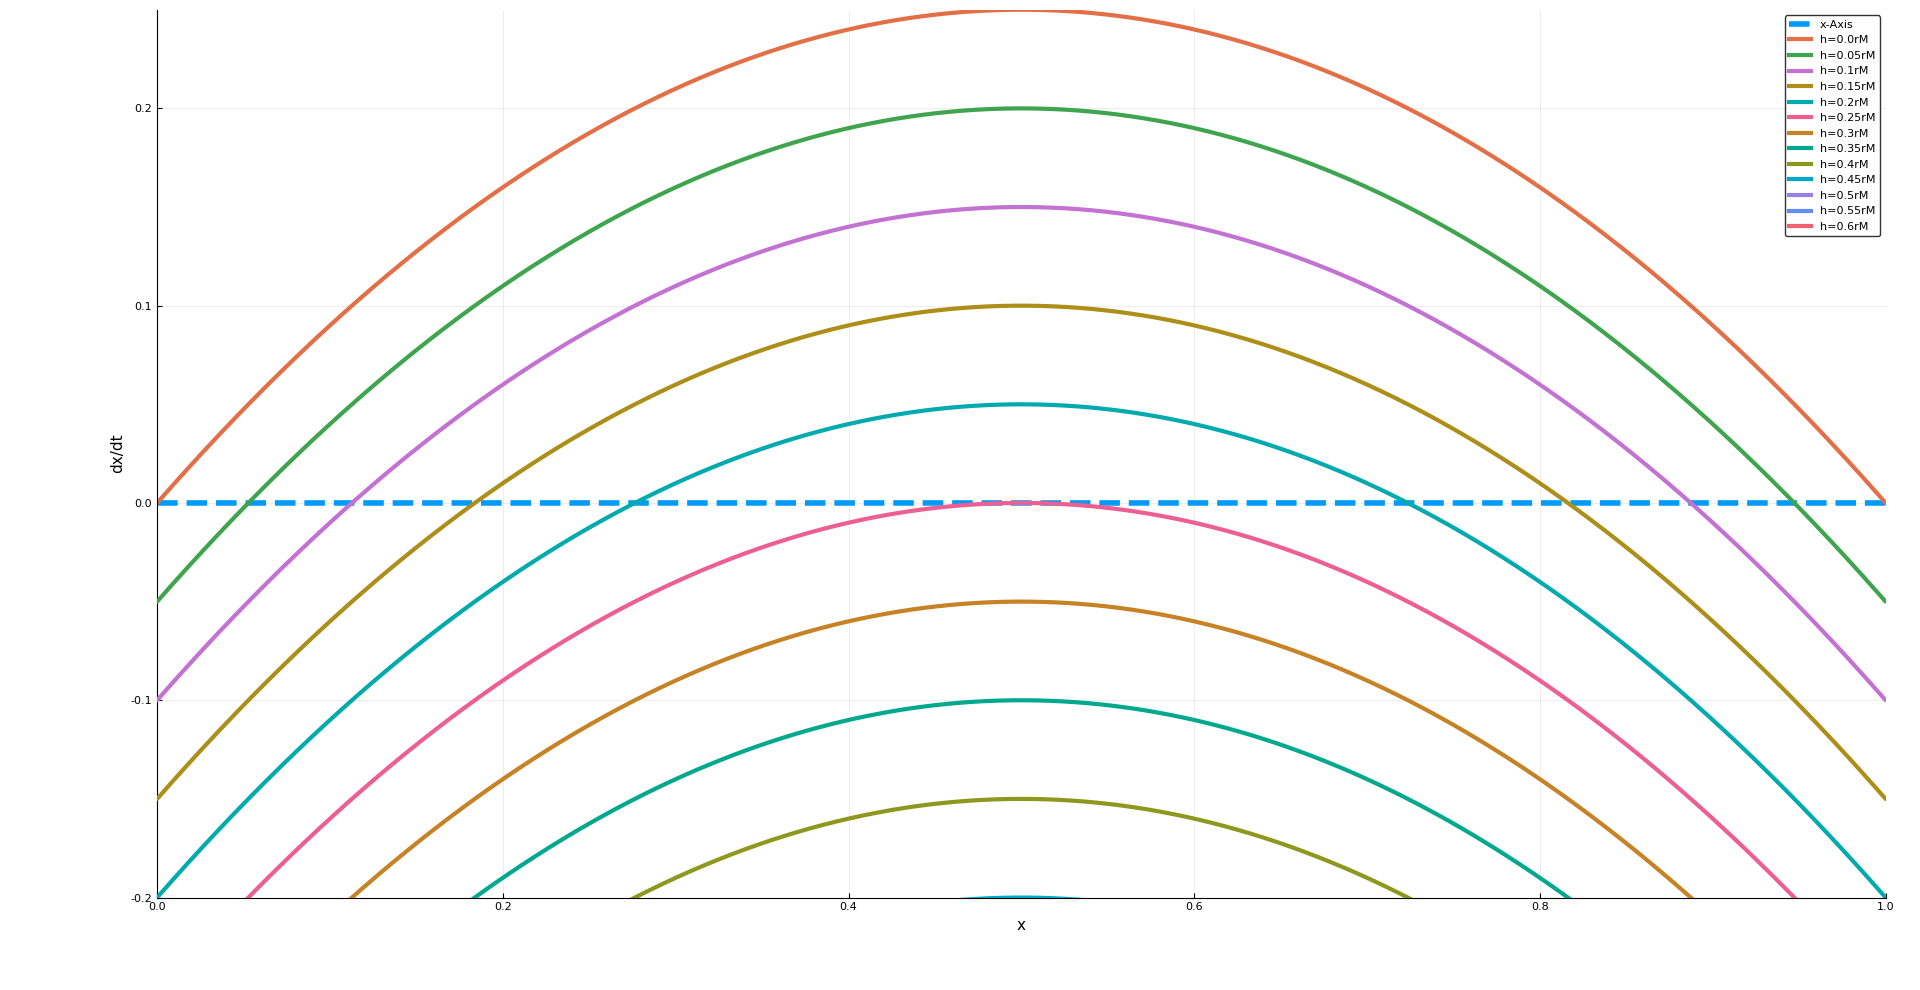
\includegraphics[width=0.8\textwidth]{CriticalPoints.png}
	\caption{Figure representing $\dev{x}{t}$ with different harvesting rates.}
	\label{fig: CriticalPoints}
\end{figure}
\begin{figure}
		\centering
		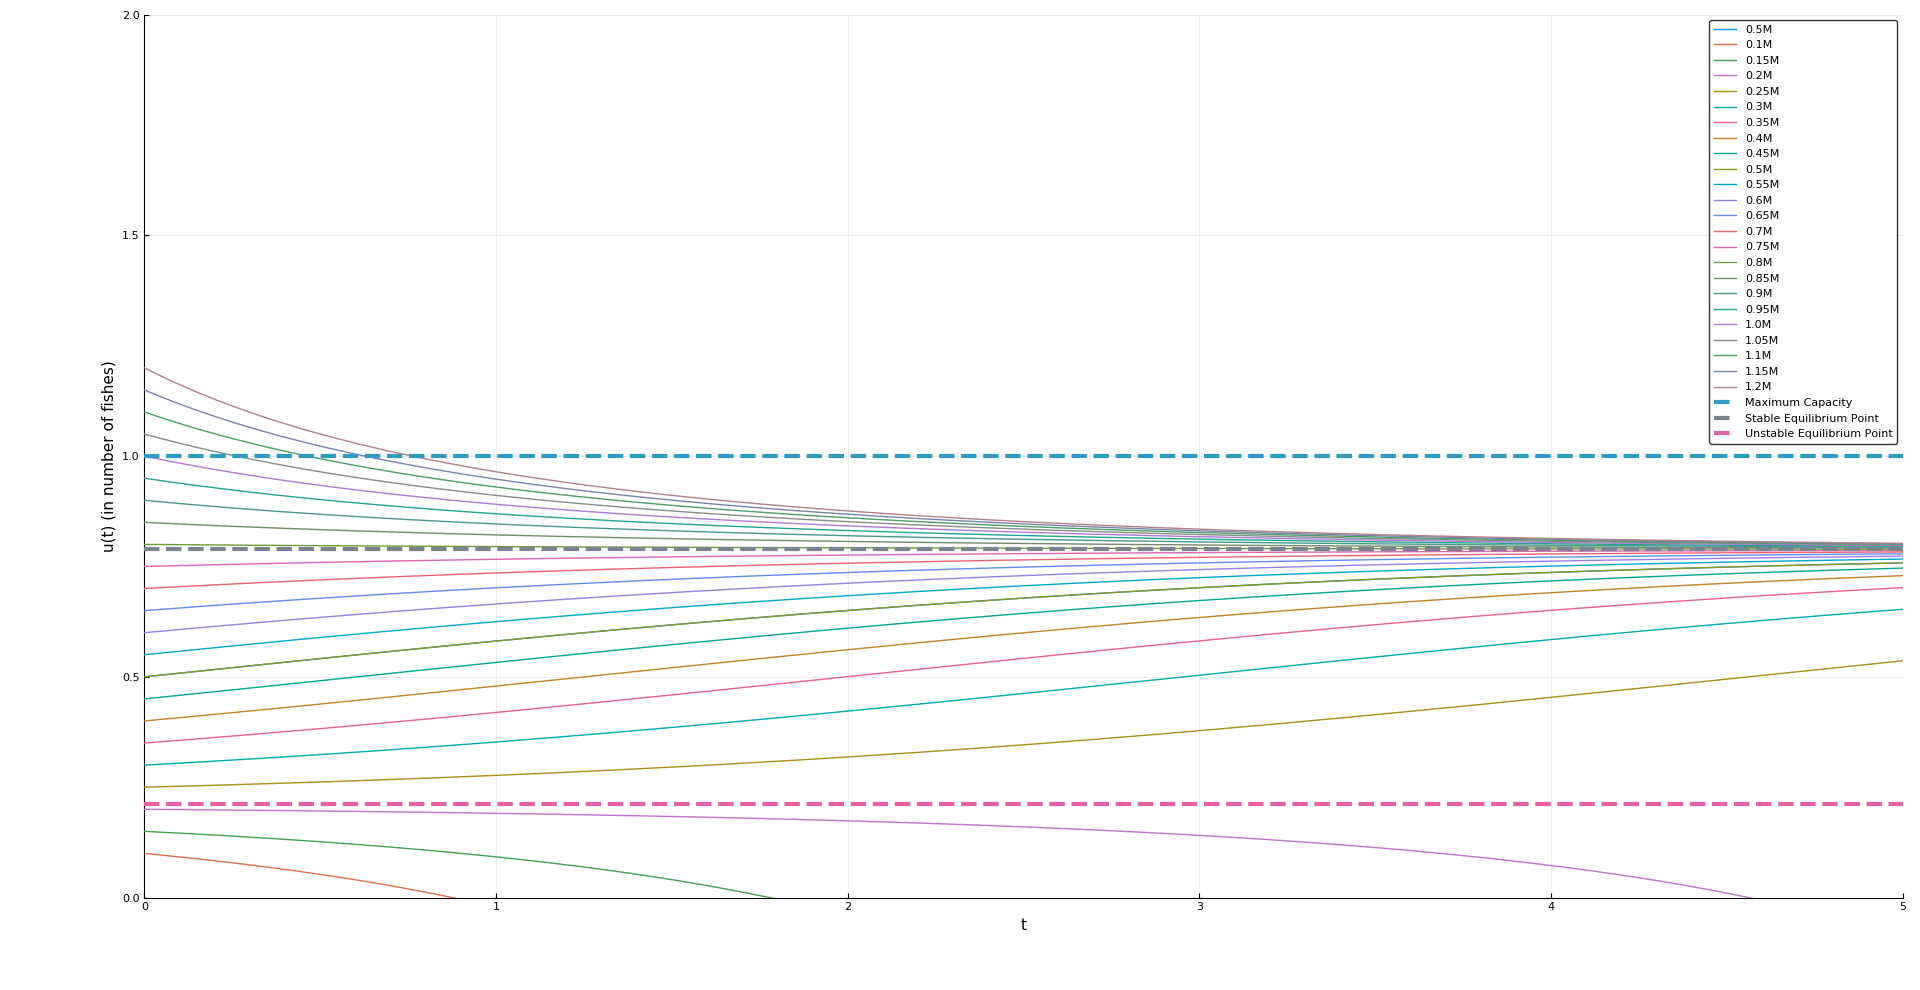
\includegraphics[width=0.8\textwidth]{SustainableConstant.png}
		\caption{Constant harvest rate $u<\frac{rM}{4}$.}
		\label{fig: SustainableConstantHarvest}
\end{figure}
\begin{figure}
	\centering
	\includegraphics[width=0.8\textwidth]{OverExploitConstant.png}
	\caption{Constant harvest rate $u>\frac{rM}{4}$.}
	\label{fig: OverExploitConstantHarvest}
\end{figure}

\begin{figure}
	\centering
	\includegraphics[width=0.8\textwidth]{CriticalExploitConstant.png}
	\caption{Constant harvest rate $u=\frac{rM}{4}$.}
	\label{fig: CriticalExploitConstantHarvest}
\end{figure}


\chapter{Economical Profit}\label{chap: Economical Profit}
	\begin{equation}
\dev{x}{t}=rx\left(1-\frac{x}{M}\right)-u \label{eq: ConstantHarvest}
\end{equation}
We introduce the following variable in order to simply calculations,
\begin{equation}
\beta=\frac{uM}{r}
\end{equation}
Solving the differential equation,
\begin{align*}
	\frac{\diff{x}}{rx\left(1-\frac{x}{M}\right)-u}&=\diff{t} \\
	\int_{x_0}^{x}\frac{\diff{\chi}}{r\chi\left(1-\frac{\chi}{M}\right)-u}&=\int_{0}^{t}\diff{\tau} \\
	\frac{M}{r}\int_{x_0}^{x}\frac{\diff{\chi}}{\chi\left(M-\chi\right)-\frac{Mu}{r}}&=t \\
	-\frac{M}{r}\int_{x_0}^{x}\frac{\diff{\chi}}{\chi^2-M\chi+\beta}&=t \nonumber
	\end{align*}
Finally, we model the above integral as one 
\begin{align}
	-\frac{M}{r}\int_{x_0}^{x}\frac{\diff{\chi}}{\left(\chi-\frac{M}{2}\right)^2-\frac{M^2}{4}+\beta}&=t
\end{align}
Consider $\alpha$ as follows,
\begin{equation}
	\alpha = \beta - \frac{M^2}{4} = rM\left(u-\frac{rM}{4}\right)
\end{equation}
We see that the sign of $\alpha$ determines the nature of the solutions. Then, if $u>rM/4$ implies $\alpha>0$,
\begin{align*}
\int_{x_0}^{x}\frac{\diff{\chi}}{\left(\chi-\frac{M}{2}\right)^2+\alpha}&=-\frac{r}{M}t \\
\frac{1}{\sqrt{\beta-\frac{M^2}{4}}}\left(\arctan\left(\frac{x-M/2}{\sqrt{\beta-M^2/4}}\right)-\arctan\left(\frac{x_0-M/2}{\sqrt{\beta-M^2/4}}\right)\right)&=-\frac{r}{M}t \\
\end{align*}
Therefore, for $\alpha > 0$ the population behaves as follows, 
\begin{align}
	x(t)=\frac{M}{2}+\sqrt{\beta-\frac{M^2}{4}} \tan \left(\arctan\left(\frac{x_0-M/2}{\sqrt{\beta-M^2/4}}\right)-\frac{r\sqrt{\beta-M^2/4}}{M}t\right) \label{eq: ConstantHarvest OverExploit}
\end{align}

Equation \ref{eq: ConstantHarvest OverExploit} show us that for some $t^*$, $x(t^*)=0$,independently of the initial condition $x_0$, since the argument inside the $\tan$ is monotone decreasing in $t$. 

If $u<rM/4$ implies $-\alpha>0$,
\begin{align*}
	\int_{x_0}^{x}\frac{\diff{\chi}}{\left(\chi-\frac{M}{2}\right)^2-(-\alpha)} &=-\frac{r}{M}t
\end{align*}
Considering the zeros of the denominator, $\lambda$ and $\overleftarrow{\lambda}$, 
\begin{equation}
	\begin{array}{cc}
	\lambda&=\frac{M}{2}+\sqrt{\frac{M^2}{4}-\beta} \\
	\overline{\lambda}&=\frac{M}{2}-\sqrt{\frac{M^2}{4}-\beta} \\
	\end{array}
\end{equation}
We can rewrite our expression as follows, 
\begin{align*}
\int_{x_0}^{x} \left(\frac{1}{\chi - \lambda}-\frac{1}{\chi - \overline{\lambda}}\right)\diff{\chi} &=-\frac{2r\sqrt{M^2/4-\beta}}{M}t \\
	\ln\abs{\frac{x - \lambda}{x - \overline{\lambda}}}&=\ln\abs{\frac{x_0- \lambda}{x_0 - \overline{\lambda}}}-\frac{2r\sqrt{M^2/4-\beta}}{M}t
\end{align*}
For simplifying calculations, we write, $\gamma=\frac{2r\sqrt{M^2/4-\beta}}{M}$. And we obtain as result,
\begin{align}
\frac{x - \lambda}{x - \overline{\lambda}} &=\frac{x_0- \lambda}{x_0- \overline{\lambda}}\mathrm e^{-\gamma t} \\
x-\lambda &=\left(x-\overline{\lambda}\right)\left(\frac{x_0- \lambda}{x_0- \overline{\lambda}}\right)\mathrm e^{-\gamma t}
\end{align}

For the sake of simplicity, consider $\xi=\frac{x_0-\lambda}{x_0-\overline{\lambda}}\mathrm{e}^{-\gamma t}$. Therefore,
\begin{align*}
	x\left(1-\xi\right)&=\lambda-\overline{\lambda}\xi\\
	x&=\frac{\lambda-\overline{\lambda}\xi}{1-\xi} \\	
	x&=\frac{\frac{M}{2}+\sqrt{\frac{M^2}{4}-\beta}-\left(\frac{M}{2}-\sqrt{\frac{M^2}{4}-\beta}\right)\xi}{1-\xi}\\
	x&=\frac{\frac{M}{2}+\sqrt{\frac{M^2}{4}-\beta}-\left(\frac{M}{2}-\sqrt{\frac{M^2}{4}-\beta}\right)\xi}{1-\xi}\\
	x&=\frac{\frac{M}{2}\left(1-\xi\right)+\sqrt{\frac{M^2}{4}-\beta}\left(1+\xi\right)}{1-\xi}\\
	x&=\frac{M}{2}+\sqrt{\frac{M^2}{4}-\beta}\frac{1+\xi}{1-\xi}
\end{align*}
Hence, for $-\alpha>0$, we have the following result,
\begin{align}
	x(t)&=\frac{M}{2}+\left(\sqrt{\frac{M^2}{4}-\beta}\right)\frac{\left(x_0-M/2\right)\left(1+\mathrm e^{-\gamma t}\right)-\sqrt{M^2/4-\beta}\left(1-\mathrm{e}^{-\gamma t}\right)}{\left(x_0-M/2\right)\left(1-\mathrm e^{-\gamma t}\right)+\sqrt{M^2/4-\beta}\left(1+\mathrm{e}^{-\gamma t}\right)} \label{eq: Time Expression for Harvest}
\end{align}

If $u=\frac{rM}{4}$, we solve equation \ref{eq: ConstantHarvest} as follows,
\begin{align}
-\frac{M}{r}\int_{x_0}^{x}\frac{d\chi}{\left(\chi-\frac{M}{2}\right)^2}&=t\\
\int_{x_0}^{x}\frac{d\chi}{\left(\chi-\frac{M}{2}\right)^2}&=-\frac{rt}{M}\\
\frac{1}{x-\frac{M}{2}}&=\frac{1}{x_0-\frac{M}{2}}-\frac{rt}{M}\\
\frac{1}{x-\frac{M}{2}}&=\frac{M-\left(x_0-\frac{M}{2}\right)rt}{M\left(x_0-\frac{M}{2}\right)} \\
x&=\frac{M}{2}+\frac{M\left(x_0-\frac{M}{2}\right)}{M-\left(x_0-\frac{M}{2}\right)rt} 
\end{align}

The results above stated can be explained directly from the equation \ref{eq: ConstantHarvest}, as we see in the graph \ref{fig: CriticalPoints},  $F(x,t)$ is a paraboloid, with its maximum at $F(x^*=M/2,t)=rM^2/4$.

When $u=0$, we have the regular logistic equation with critical points $x_{c_1}=0$ and $x_{c_2}=M$. With $x_{c_2}$ being an stable fixed point and $x_{c_1}$ an unstable fixed point. In general, these are the solutions to the equation $F(x,t)-u=0$,
\begin{equation}
x_{c_{2,1}}=\frac{M}{2}\pm \sqrt{\frac{M^2}{4}-u\frac{M}{r}}
\end{equation}

We observe that the critical points $x_c$, such that $\dev{x_c}{t}=F(x_c, t)-u=0$ are getting closer to each other, as $u$ is increasing; when $u=\frac{rM}{4}$ we only have one critical unstable point. That behaves as an attractor when $x_0\geq\frac{M}{2}$. But when $x_0<\frac{M}{2}$ the population strictly decreases. For $u> \frac{rM}{4}$, the population $x(t)$ has no real critical points and the derivative $\dev{x}{t}$ is always negative, implying, that we will lead always the population to extinction, extracting constantly at a rate greater than $\frac{rM}{4}$.

\begin{figure}[H]
	\centering
	\includegraphics[width=0.8\textwidth]{CriticalPoints.png}
	\caption{Figure representing $\dev{x}{t}$ with different harvesting rates.}
	\label{fig: CriticalPoints}
\end{figure}
\begin{figure}
		\centering
		\includegraphics[width=0.8\textwidth]{SustainableConstant.png}
		\caption{Constant harvest rate $u<\frac{rM}{4}$.}
		\label{fig: SustainableConstantHarvest}
\end{figure}
\begin{figure}
	\centering
	\includegraphics[width=0.8\textwidth]{OverExploitConstant.png}
	\caption{Constant harvest rate $u>\frac{rM}{4}$.}
	\label{fig: OverExploitConstantHarvest}
\end{figure}

\begin{figure}
	\centering
	\includegraphics[width=0.8\textwidth]{CriticalExploitConstant.png}
	\caption{Constant harvest rate $u=\frac{rM}{4}$.}
	\label{fig: CriticalExploitConstantHarvest}
\end{figure}


	\section{Linear Costs.}
	\begin{equation}
\dev{x}{t}=rx\left(1-\frac{x}{M}\right)-u \label{eq: ConstantHarvest}
\end{equation}
We introduce the following variable in order to simply calculations,
\begin{equation}
\beta=\frac{uM}{r}
\end{equation}
Solving the differential equation,
\begin{align*}
	\frac{\diff{x}}{rx\left(1-\frac{x}{M}\right)-u}&=\diff{t} \\
	\int_{x_0}^{x}\frac{\diff{\chi}}{r\chi\left(1-\frac{\chi}{M}\right)-u}&=\int_{0}^{t}\diff{\tau} \\
	\frac{M}{r}\int_{x_0}^{x}\frac{\diff{\chi}}{\chi\left(M-\chi\right)-\frac{Mu}{r}}&=t \\
	-\frac{M}{r}\int_{x_0}^{x}\frac{\diff{\chi}}{\chi^2-M\chi+\beta}&=t \nonumber
	\end{align*}
Finally, we model the above integral as one 
\begin{align}
	-\frac{M}{r}\int_{x_0}^{x}\frac{\diff{\chi}}{\left(\chi-\frac{M}{2}\right)^2-\frac{M^2}{4}+\beta}&=t
\end{align}
Consider $\alpha$ as follows,
\begin{equation}
	\alpha = \beta - \frac{M^2}{4} = rM\left(u-\frac{rM}{4}\right)
\end{equation}
We see that the sign of $\alpha$ determines the nature of the solutions. Then, if $u>rM/4$ implies $\alpha>0$,
\begin{align*}
\int_{x_0}^{x}\frac{\diff{\chi}}{\left(\chi-\frac{M}{2}\right)^2+\alpha}&=-\frac{r}{M}t \\
\frac{1}{\sqrt{\beta-\frac{M^2}{4}}}\left(\arctan\left(\frac{x-M/2}{\sqrt{\beta-M^2/4}}\right)-\arctan\left(\frac{x_0-M/2}{\sqrt{\beta-M^2/4}}\right)\right)&=-\frac{r}{M}t \\
\end{align*}
Therefore, for $\alpha > 0$ the population behaves as follows, 
\begin{align}
	x(t)=\frac{M}{2}+\sqrt{\beta-\frac{M^2}{4}} \tan \left(\arctan\left(\frac{x_0-M/2}{\sqrt{\beta-M^2/4}}\right)-\frac{r\sqrt{\beta-M^2/4}}{M}t\right) \label{eq: ConstantHarvest OverExploit}
\end{align}

Equation \ref{eq: ConstantHarvest OverExploit} show us that for some $t^*$, $x(t^*)=0$,independently of the initial condition $x_0$, since the argument inside the $\tan$ is monotone decreasing in $t$. 

If $u<rM/4$ implies $-\alpha>0$,
\begin{align*}
	\int_{x_0}^{x}\frac{\diff{\chi}}{\left(\chi-\frac{M}{2}\right)^2-(-\alpha)} &=-\frac{r}{M}t
\end{align*}
Considering the zeros of the denominator, $\lambda$ and $\overleftarrow{\lambda}$, 
\begin{equation}
	\begin{array}{cc}
	\lambda&=\frac{M}{2}+\sqrt{\frac{M^2}{4}-\beta} \\
	\overline{\lambda}&=\frac{M}{2}-\sqrt{\frac{M^2}{4}-\beta} \\
	\end{array}
\end{equation}
We can rewrite our expression as follows, 
\begin{align*}
\int_{x_0}^{x} \left(\frac{1}{\chi - \lambda}-\frac{1}{\chi - \overline{\lambda}}\right)\diff{\chi} &=-\frac{2r\sqrt{M^2/4-\beta}}{M}t \\
	\ln\abs{\frac{x - \lambda}{x - \overline{\lambda}}}&=\ln\abs{\frac{x_0- \lambda}{x_0 - \overline{\lambda}}}-\frac{2r\sqrt{M^2/4-\beta}}{M}t
\end{align*}
For simplifying calculations, we write, $\gamma=\frac{2r\sqrt{M^2/4-\beta}}{M}$. And we obtain as result,
\begin{align}
\frac{x - \lambda}{x - \overline{\lambda}} &=\frac{x_0- \lambda}{x_0- \overline{\lambda}}\mathrm e^{-\gamma t} \\
x-\lambda &=\left(x-\overline{\lambda}\right)\left(\frac{x_0- \lambda}{x_0- \overline{\lambda}}\right)\mathrm e^{-\gamma t}
\end{align}

For the sake of simplicity, consider $\xi=\frac{x_0-\lambda}{x_0-\overline{\lambda}}\mathrm{e}^{-\gamma t}$. Therefore,
\begin{align*}
	x\left(1-\xi\right)&=\lambda-\overline{\lambda}\xi\\
	x&=\frac{\lambda-\overline{\lambda}\xi}{1-\xi} \\	
	x&=\frac{\frac{M}{2}+\sqrt{\frac{M^2}{4}-\beta}-\left(\frac{M}{2}-\sqrt{\frac{M^2}{4}-\beta}\right)\xi}{1-\xi}\\
	x&=\frac{\frac{M}{2}+\sqrt{\frac{M^2}{4}-\beta}-\left(\frac{M}{2}-\sqrt{\frac{M^2}{4}-\beta}\right)\xi}{1-\xi}\\
	x&=\frac{\frac{M}{2}\left(1-\xi\right)+\sqrt{\frac{M^2}{4}-\beta}\left(1+\xi\right)}{1-\xi}\\
	x&=\frac{M}{2}+\sqrt{\frac{M^2}{4}-\beta}\frac{1+\xi}{1-\xi}
\end{align*}
Hence, for $-\alpha>0$, we have the following result,
\begin{align}
	x(t)&=\frac{M}{2}+\left(\sqrt{\frac{M^2}{4}-\beta}\right)\frac{\left(x_0-M/2\right)\left(1+\mathrm e^{-\gamma t}\right)-\sqrt{M^2/4-\beta}\left(1-\mathrm{e}^{-\gamma t}\right)}{\left(x_0-M/2\right)\left(1-\mathrm e^{-\gamma t}\right)+\sqrt{M^2/4-\beta}\left(1+\mathrm{e}^{-\gamma t}\right)} \label{eq: Time Expression for Harvest}
\end{align}

If $u=\frac{rM}{4}$, we solve equation \ref{eq: ConstantHarvest} as follows,
\begin{align}
-\frac{M}{r}\int_{x_0}^{x}\frac{d\chi}{\left(\chi-\frac{M}{2}\right)^2}&=t\\
\int_{x_0}^{x}\frac{d\chi}{\left(\chi-\frac{M}{2}\right)^2}&=-\frac{rt}{M}\\
\frac{1}{x-\frac{M}{2}}&=\frac{1}{x_0-\frac{M}{2}}-\frac{rt}{M}\\
\frac{1}{x-\frac{M}{2}}&=\frac{M-\left(x_0-\frac{M}{2}\right)rt}{M\left(x_0-\frac{M}{2}\right)} \\
x&=\frac{M}{2}+\frac{M\left(x_0-\frac{M}{2}\right)}{M-\left(x_0-\frac{M}{2}\right)rt} 
\end{align}

The results above stated can be explained directly from the equation \ref{eq: ConstantHarvest}, as we see in the graph \ref{fig: CriticalPoints},  $F(x,t)$ is a paraboloid, with its maximum at $F(x^*=M/2,t)=rM^2/4$.

When $u=0$, we have the regular logistic equation with critical points $x_{c_1}=0$ and $x_{c_2}=M$. With $x_{c_2}$ being an stable fixed point and $x_{c_1}$ an unstable fixed point. In general, these are the solutions to the equation $F(x,t)-u=0$,
\begin{equation}
x_{c_{2,1}}=\frac{M}{2}\pm \sqrt{\frac{M^2}{4}-u\frac{M}{r}}
\end{equation}

We observe that the critical points $x_c$, such that $\dev{x_c}{t}=F(x_c, t)-u=0$ are getting closer to each other, as $u$ is increasing; when $u=\frac{rM}{4}$ we only have one critical unstable point. That behaves as an attractor when $x_0\geq\frac{M}{2}$. But when $x_0<\frac{M}{2}$ the population strictly decreases. For $u> \frac{rM}{4}$, the population $x(t)$ has no real critical points and the derivative $\dev{x}{t}$ is always negative, implying, that we will lead always the population to extinction, extracting constantly at a rate greater than $\frac{rM}{4}$.

\begin{figure}[H]
	\centering
	\includegraphics[width=0.8\textwidth]{CriticalPoints.png}
	\caption{Figure representing $\dev{x}{t}$ with different harvesting rates.}
	\label{fig: CriticalPoints}
\end{figure}
\begin{figure}
		\centering
		\includegraphics[width=0.8\textwidth]{SustainableConstant.png}
		\caption{Constant harvest rate $u<\frac{rM}{4}$.}
		\label{fig: SustainableConstantHarvest}
\end{figure}
\begin{figure}
	\centering
	\includegraphics[width=0.8\textwidth]{OverExploitConstant.png}
	\caption{Constant harvest rate $u>\frac{rM}{4}$.}
	\label{fig: OverExploitConstantHarvest}
\end{figure}

\begin{figure}
	\centering
	\includegraphics[width=0.8\textwidth]{CriticalExploitConstant.png}
	\caption{Constant harvest rate $u=\frac{rM}{4}$.}
	\label{fig: CriticalExploitConstantHarvest}
\end{figure}


	\section{Dynamic Programming.}
	\begin{equation}
\dev{x}{t}=rx\left(1-\frac{x}{M}\right)-u \label{eq: ConstantHarvest}
\end{equation}
We introduce the following variable in order to simply calculations,
\begin{equation}
\beta=\frac{uM}{r}
\end{equation}
Solving the differential equation,
\begin{align*}
	\frac{\diff{x}}{rx\left(1-\frac{x}{M}\right)-u}&=\diff{t} \\
	\int_{x_0}^{x}\frac{\diff{\chi}}{r\chi\left(1-\frac{\chi}{M}\right)-u}&=\int_{0}^{t}\diff{\tau} \\
	\frac{M}{r}\int_{x_0}^{x}\frac{\diff{\chi}}{\chi\left(M-\chi\right)-\frac{Mu}{r}}&=t \\
	-\frac{M}{r}\int_{x_0}^{x}\frac{\diff{\chi}}{\chi^2-M\chi+\beta}&=t \nonumber
	\end{align*}
Finally, we model the above integral as one 
\begin{align}
	-\frac{M}{r}\int_{x_0}^{x}\frac{\diff{\chi}}{\left(\chi-\frac{M}{2}\right)^2-\frac{M^2}{4}+\beta}&=t
\end{align}
Consider $\alpha$ as follows,
\begin{equation}
	\alpha = \beta - \frac{M^2}{4} = rM\left(u-\frac{rM}{4}\right)
\end{equation}
We see that the sign of $\alpha$ determines the nature of the solutions. Then, if $u>rM/4$ implies $\alpha>0$,
\begin{align*}
\int_{x_0}^{x}\frac{\diff{\chi}}{\left(\chi-\frac{M}{2}\right)^2+\alpha}&=-\frac{r}{M}t \\
\frac{1}{\sqrt{\beta-\frac{M^2}{4}}}\left(\arctan\left(\frac{x-M/2}{\sqrt{\beta-M^2/4}}\right)-\arctan\left(\frac{x_0-M/2}{\sqrt{\beta-M^2/4}}\right)\right)&=-\frac{r}{M}t \\
\end{align*}
Therefore, for $\alpha > 0$ the population behaves as follows, 
\begin{align}
	x(t)=\frac{M}{2}+\sqrt{\beta-\frac{M^2}{4}} \tan \left(\arctan\left(\frac{x_0-M/2}{\sqrt{\beta-M^2/4}}\right)-\frac{r\sqrt{\beta-M^2/4}}{M}t\right) \label{eq: ConstantHarvest OverExploit}
\end{align}

Equation \ref{eq: ConstantHarvest OverExploit} show us that for some $t^*$, $x(t^*)=0$,independently of the initial condition $x_0$, since the argument inside the $\tan$ is monotone decreasing in $t$. 

If $u<rM/4$ implies $-\alpha>0$,
\begin{align*}
	\int_{x_0}^{x}\frac{\diff{\chi}}{\left(\chi-\frac{M}{2}\right)^2-(-\alpha)} &=-\frac{r}{M}t
\end{align*}
Considering the zeros of the denominator, $\lambda$ and $\overleftarrow{\lambda}$, 
\begin{equation}
	\begin{array}{cc}
	\lambda&=\frac{M}{2}+\sqrt{\frac{M^2}{4}-\beta} \\
	\overline{\lambda}&=\frac{M}{2}-\sqrt{\frac{M^2}{4}-\beta} \\
	\end{array}
\end{equation}
We can rewrite our expression as follows, 
\begin{align*}
\int_{x_0}^{x} \left(\frac{1}{\chi - \lambda}-\frac{1}{\chi - \overline{\lambda}}\right)\diff{\chi} &=-\frac{2r\sqrt{M^2/4-\beta}}{M}t \\
	\ln\abs{\frac{x - \lambda}{x - \overline{\lambda}}}&=\ln\abs{\frac{x_0- \lambda}{x_0 - \overline{\lambda}}}-\frac{2r\sqrt{M^2/4-\beta}}{M}t
\end{align*}
For simplifying calculations, we write, $\gamma=\frac{2r\sqrt{M^2/4-\beta}}{M}$. And we obtain as result,
\begin{align}
\frac{x - \lambda}{x - \overline{\lambda}} &=\frac{x_0- \lambda}{x_0- \overline{\lambda}}\mathrm e^{-\gamma t} \\
x-\lambda &=\left(x-\overline{\lambda}\right)\left(\frac{x_0- \lambda}{x_0- \overline{\lambda}}\right)\mathrm e^{-\gamma t}
\end{align}

For the sake of simplicity, consider $\xi=\frac{x_0-\lambda}{x_0-\overline{\lambda}}\mathrm{e}^{-\gamma t}$. Therefore,
\begin{align*}
	x\left(1-\xi\right)&=\lambda-\overline{\lambda}\xi\\
	x&=\frac{\lambda-\overline{\lambda}\xi}{1-\xi} \\	
	x&=\frac{\frac{M}{2}+\sqrt{\frac{M^2}{4}-\beta}-\left(\frac{M}{2}-\sqrt{\frac{M^2}{4}-\beta}\right)\xi}{1-\xi}\\
	x&=\frac{\frac{M}{2}+\sqrt{\frac{M^2}{4}-\beta}-\left(\frac{M}{2}-\sqrt{\frac{M^2}{4}-\beta}\right)\xi}{1-\xi}\\
	x&=\frac{\frac{M}{2}\left(1-\xi\right)+\sqrt{\frac{M^2}{4}-\beta}\left(1+\xi\right)}{1-\xi}\\
	x&=\frac{M}{2}+\sqrt{\frac{M^2}{4}-\beta}\frac{1+\xi}{1-\xi}
\end{align*}
Hence, for $-\alpha>0$, we have the following result,
\begin{align}
	x(t)&=\frac{M}{2}+\left(\sqrt{\frac{M^2}{4}-\beta}\right)\frac{\left(x_0-M/2\right)\left(1+\mathrm e^{-\gamma t}\right)-\sqrt{M^2/4-\beta}\left(1-\mathrm{e}^{-\gamma t}\right)}{\left(x_0-M/2\right)\left(1-\mathrm e^{-\gamma t}\right)+\sqrt{M^2/4-\beta}\left(1+\mathrm{e}^{-\gamma t}\right)} \label{eq: Time Expression for Harvest}
\end{align}

If $u=\frac{rM}{4}$, we solve equation \ref{eq: ConstantHarvest} as follows,
\begin{align}
-\frac{M}{r}\int_{x_0}^{x}\frac{d\chi}{\left(\chi-\frac{M}{2}\right)^2}&=t\\
\int_{x_0}^{x}\frac{d\chi}{\left(\chi-\frac{M}{2}\right)^2}&=-\frac{rt}{M}\\
\frac{1}{x-\frac{M}{2}}&=\frac{1}{x_0-\frac{M}{2}}-\frac{rt}{M}\\
\frac{1}{x-\frac{M}{2}}&=\frac{M-\left(x_0-\frac{M}{2}\right)rt}{M\left(x_0-\frac{M}{2}\right)} \\
x&=\frac{M}{2}+\frac{M\left(x_0-\frac{M}{2}\right)}{M-\left(x_0-\frac{M}{2}\right)rt} 
\end{align}

The results above stated can be explained directly from the equation \ref{eq: ConstantHarvest}, as we see in the graph \ref{fig: CriticalPoints},  $F(x,t)$ is a paraboloid, with its maximum at $F(x^*=M/2,t)=rM^2/4$.

When $u=0$, we have the regular logistic equation with critical points $x_{c_1}=0$ and $x_{c_2}=M$. With $x_{c_2}$ being an stable fixed point and $x_{c_1}$ an unstable fixed point. In general, these are the solutions to the equation $F(x,t)-u=0$,
\begin{equation}
x_{c_{2,1}}=\frac{M}{2}\pm \sqrt{\frac{M^2}{4}-u\frac{M}{r}}
\end{equation}

We observe that the critical points $x_c$, such that $\dev{x_c}{t}=F(x_c, t)-u=0$ are getting closer to each other, as $u$ is increasing; when $u=\frac{rM}{4}$ we only have one critical unstable point. That behaves as an attractor when $x_0\geq\frac{M}{2}$. But when $x_0<\frac{M}{2}$ the population strictly decreases. For $u> \frac{rM}{4}$, the population $x(t)$ has no real critical points and the derivative $\dev{x}{t}$ is always negative, implying, that we will lead always the population to extinction, extracting constantly at a rate greater than $\frac{rM}{4}$.

\begin{figure}[H]
	\centering
	\includegraphics[width=0.8\textwidth]{CriticalPoints.png}
	\caption{Figure representing $\dev{x}{t}$ with different harvesting rates.}
	\label{fig: CriticalPoints}
\end{figure}
\begin{figure}
		\centering
		\includegraphics[width=0.8\textwidth]{SustainableConstant.png}
		\caption{Constant harvest rate $u<\frac{rM}{4}$.}
		\label{fig: SustainableConstantHarvest}
\end{figure}
\begin{figure}
	\centering
	\includegraphics[width=0.8\textwidth]{OverExploitConstant.png}
	\caption{Constant harvest rate $u>\frac{rM}{4}$.}
	\label{fig: OverExploitConstantHarvest}
\end{figure}

\begin{figure}
	\centering
	\includegraphics[width=0.8\textwidth]{CriticalExploitConstant.png}
	\caption{Constant harvest rate $u=\frac{rM}{4}$.}
	\label{fig: CriticalExploitConstantHarvest}
\end{figure}


	\section{Stochastic Analysis.}
	\begin{equation}
\dev{x}{t}=rx\left(1-\frac{x}{M}\right)-u \label{eq: ConstantHarvest}
\end{equation}
We introduce the following variable in order to simply calculations,
\begin{equation}
\beta=\frac{uM}{r}
\end{equation}
Solving the differential equation,
\begin{align*}
	\frac{\diff{x}}{rx\left(1-\frac{x}{M}\right)-u}&=\diff{t} \\
	\int_{x_0}^{x}\frac{\diff{\chi}}{r\chi\left(1-\frac{\chi}{M}\right)-u}&=\int_{0}^{t}\diff{\tau} \\
	\frac{M}{r}\int_{x_0}^{x}\frac{\diff{\chi}}{\chi\left(M-\chi\right)-\frac{Mu}{r}}&=t \\
	-\frac{M}{r}\int_{x_0}^{x}\frac{\diff{\chi}}{\chi^2-M\chi+\beta}&=t \nonumber
	\end{align*}
Finally, we model the above integral as one 
\begin{align}
	-\frac{M}{r}\int_{x_0}^{x}\frac{\diff{\chi}}{\left(\chi-\frac{M}{2}\right)^2-\frac{M^2}{4}+\beta}&=t
\end{align}
Consider $\alpha$ as follows,
\begin{equation}
	\alpha = \beta - \frac{M^2}{4} = rM\left(u-\frac{rM}{4}\right)
\end{equation}
We see that the sign of $\alpha$ determines the nature of the solutions. Then, if $u>rM/4$ implies $\alpha>0$,
\begin{align*}
\int_{x_0}^{x}\frac{\diff{\chi}}{\left(\chi-\frac{M}{2}\right)^2+\alpha}&=-\frac{r}{M}t \\
\frac{1}{\sqrt{\beta-\frac{M^2}{4}}}\left(\arctan\left(\frac{x-M/2}{\sqrt{\beta-M^2/4}}\right)-\arctan\left(\frac{x_0-M/2}{\sqrt{\beta-M^2/4}}\right)\right)&=-\frac{r}{M}t \\
\end{align*}
Therefore, for $\alpha > 0$ the population behaves as follows, 
\begin{align}
	x(t)=\frac{M}{2}+\sqrt{\beta-\frac{M^2}{4}} \tan \left(\arctan\left(\frac{x_0-M/2}{\sqrt{\beta-M^2/4}}\right)-\frac{r\sqrt{\beta-M^2/4}}{M}t\right) \label{eq: ConstantHarvest OverExploit}
\end{align}

Equation \ref{eq: ConstantHarvest OverExploit} show us that for some $t^*$, $x(t^*)=0$,independently of the initial condition $x_0$, since the argument inside the $\tan$ is monotone decreasing in $t$. 

If $u<rM/4$ implies $-\alpha>0$,
\begin{align*}
	\int_{x_0}^{x}\frac{\diff{\chi}}{\left(\chi-\frac{M}{2}\right)^2-(-\alpha)} &=-\frac{r}{M}t
\end{align*}
Considering the zeros of the denominator, $\lambda$ and $\overleftarrow{\lambda}$, 
\begin{equation}
	\begin{array}{cc}
	\lambda&=\frac{M}{2}+\sqrt{\frac{M^2}{4}-\beta} \\
	\overline{\lambda}&=\frac{M}{2}-\sqrt{\frac{M^2}{4}-\beta} \\
	\end{array}
\end{equation}
We can rewrite our expression as follows, 
\begin{align*}
\int_{x_0}^{x} \left(\frac{1}{\chi - \lambda}-\frac{1}{\chi - \overline{\lambda}}\right)\diff{\chi} &=-\frac{2r\sqrt{M^2/4-\beta}}{M}t \\
	\ln\abs{\frac{x - \lambda}{x - \overline{\lambda}}}&=\ln\abs{\frac{x_0- \lambda}{x_0 - \overline{\lambda}}}-\frac{2r\sqrt{M^2/4-\beta}}{M}t
\end{align*}
For simplifying calculations, we write, $\gamma=\frac{2r\sqrt{M^2/4-\beta}}{M}$. And we obtain as result,
\begin{align}
\frac{x - \lambda}{x - \overline{\lambda}} &=\frac{x_0- \lambda}{x_0- \overline{\lambda}}\mathrm e^{-\gamma t} \\
x-\lambda &=\left(x-\overline{\lambda}\right)\left(\frac{x_0- \lambda}{x_0- \overline{\lambda}}\right)\mathrm e^{-\gamma t}
\end{align}

For the sake of simplicity, consider $\xi=\frac{x_0-\lambda}{x_0-\overline{\lambda}}\mathrm{e}^{-\gamma t}$. Therefore,
\begin{align*}
	x\left(1-\xi\right)&=\lambda-\overline{\lambda}\xi\\
	x&=\frac{\lambda-\overline{\lambda}\xi}{1-\xi} \\	
	x&=\frac{\frac{M}{2}+\sqrt{\frac{M^2}{4}-\beta}-\left(\frac{M}{2}-\sqrt{\frac{M^2}{4}-\beta}\right)\xi}{1-\xi}\\
	x&=\frac{\frac{M}{2}+\sqrt{\frac{M^2}{4}-\beta}-\left(\frac{M}{2}-\sqrt{\frac{M^2}{4}-\beta}\right)\xi}{1-\xi}\\
	x&=\frac{\frac{M}{2}\left(1-\xi\right)+\sqrt{\frac{M^2}{4}-\beta}\left(1+\xi\right)}{1-\xi}\\
	x&=\frac{M}{2}+\sqrt{\frac{M^2}{4}-\beta}\frac{1+\xi}{1-\xi}
\end{align*}
Hence, for $-\alpha>0$, we have the following result,
\begin{align}
	x(t)&=\frac{M}{2}+\left(\sqrt{\frac{M^2}{4}-\beta}\right)\frac{\left(x_0-M/2\right)\left(1+\mathrm e^{-\gamma t}\right)-\sqrt{M^2/4-\beta}\left(1-\mathrm{e}^{-\gamma t}\right)}{\left(x_0-M/2\right)\left(1-\mathrm e^{-\gamma t}\right)+\sqrt{M^2/4-\beta}\left(1+\mathrm{e}^{-\gamma t}\right)} \label{eq: Time Expression for Harvest}
\end{align}

If $u=\frac{rM}{4}$, we solve equation \ref{eq: ConstantHarvest} as follows,
\begin{align}
-\frac{M}{r}\int_{x_0}^{x}\frac{d\chi}{\left(\chi-\frac{M}{2}\right)^2}&=t\\
\int_{x_0}^{x}\frac{d\chi}{\left(\chi-\frac{M}{2}\right)^2}&=-\frac{rt}{M}\\
\frac{1}{x-\frac{M}{2}}&=\frac{1}{x_0-\frac{M}{2}}-\frac{rt}{M}\\
\frac{1}{x-\frac{M}{2}}&=\frac{M-\left(x_0-\frac{M}{2}\right)rt}{M\left(x_0-\frac{M}{2}\right)} \\
x&=\frac{M}{2}+\frac{M\left(x_0-\frac{M}{2}\right)}{M-\left(x_0-\frac{M}{2}\right)rt} 
\end{align}

The results above stated can be explained directly from the equation \ref{eq: ConstantHarvest}, as we see in the graph \ref{fig: CriticalPoints},  $F(x,t)$ is a paraboloid, with its maximum at $F(x^*=M/2,t)=rM^2/4$.

When $u=0$, we have the regular logistic equation with critical points $x_{c_1}=0$ and $x_{c_2}=M$. With $x_{c_2}$ being an stable fixed point and $x_{c_1}$ an unstable fixed point. In general, these are the solutions to the equation $F(x,t)-u=0$,
\begin{equation}
x_{c_{2,1}}=\frac{M}{2}\pm \sqrt{\frac{M^2}{4}-u\frac{M}{r}}
\end{equation}

We observe that the critical points $x_c$, such that $\dev{x_c}{t}=F(x_c, t)-u=0$ are getting closer to each other, as $u$ is increasing; when $u=\frac{rM}{4}$ we only have one critical unstable point. That behaves as an attractor when $x_0\geq\frac{M}{2}$. But when $x_0<\frac{M}{2}$ the population strictly decreases. For $u> \frac{rM}{4}$, the population $x(t)$ has no real critical points and the derivative $\dev{x}{t}$ is always negative, implying, that we will lead always the population to extinction, extracting constantly at a rate greater than $\frac{rM}{4}$.

\begin{figure}[H]
	\centering
	\includegraphics[width=0.8\textwidth]{CriticalPoints.png}
	\caption{Figure representing $\dev{x}{t}$ with different harvesting rates.}
	\label{fig: CriticalPoints}
\end{figure}
\begin{figure}
		\centering
		\includegraphics[width=0.8\textwidth]{SustainableConstant.png}
		\caption{Constant harvest rate $u<\frac{rM}{4}$.}
		\label{fig: SustainableConstantHarvest}
\end{figure}
\begin{figure}
	\centering
	\includegraphics[width=0.8\textwidth]{OverExploitConstant.png}
	\caption{Constant harvest rate $u>\frac{rM}{4}$.}
	\label{fig: OverExploitConstantHarvest}
\end{figure}

\begin{figure}
	\centering
	\includegraphics[width=0.8\textwidth]{CriticalExploitConstant.png}
	\caption{Constant harvest rate $u=\frac{rM}{4}$.}
	\label{fig: CriticalExploitConstantHarvest}
\end{figure}


\chapter{Further Research}\label{chap: Further Enhancements}

\end{document}
